% docx2tex 1.7 --- ''Just out of this Word.'' 
% 
% docx2tex is Open Source and  
% you can download it on GitHub: 
% https://github.com/transpect/docx2tex 
%  
\documentclass[10pt,a4paper,titlepage,dvipdfmx]{book}
\usepackage[T1]{fontenc} 
%\usepackage[utf8]{inputenc} 
%\usepackage{graphicx}
\usepackage{hyperref} 
\usepackage{multirow} 
\usepackage{tabularx} 
%\usepackage{color} 
\usepackage[dvipdfmx]{color}
\usepackage{textcomp} 
\usepackage{tipa}
\usepackage{amsmath} 
\usepackage{amssymb} 
\usepackage{amsfonts} 
\usepackage{amsxtra} 
\usepackage{wasysym} 
\usepackage{isomath} 
\usepackage{mathtools} 
\usepackage{txfonts} 
\usepackage{upgreek} 
\usepackage{enumerate} 
\usepackage{tensor} 
\usepackage{pifont} 
\usepackage{ulem} 
\usepackage{xfrac} 
\usepackage{soul}
\usepackage{seqsplit}
%\usepackage{arydshln} 
\usepackage{ltablex}
%\usepackage{longtable}
\usepackage{graphicx}
%\usepackage[ngerman,english]{babel}
\usepackage{autobreak}
\usepackage{pdflscape}
\definecolor{color-1}{rgb}{0.99,0.84,0.71}
\definecolor{color-2}{rgb}{1,1,1}
\definecolor{color-3}{rgb}{1,0,0}
\definecolor{color-4}{rgb}{1,1,0}
\definecolor{color-5}{rgb}{0,1,0}
\definecolor{color-6}{rgb}{1,0.75,0}
\definecolor{color-7}{rgb}{0,0,1}
\definecolor{color-8}{rgb}{0.64,0.08,0.08}
\setlongtables

\title{AIM/Hub 2.3.19 Documentation}
\author{Shinichiro Fujimori}



\begin{document}

\maketitle

\begin{flushleft}
Authors: Shinichiro Fujimori\textsuperscript{1,2*} \linebreak\linebreak\linebreak\\

\textsuperscript{1} Department of Urban and Environmental Engineering, Kyoto University

Postal address: 367, C1-3, Kyoto-daigaku Katsura campus, Nishikyo-ku, Kyoto city, Kyoto, 606-8540, Japan 

\textsuperscript{2} Center for Social and Environmental Systems Research, National institute for environmental studies

Postal address: National institute for environmental studies, 16-2 Onogawa, Tsukuba, Ibaraki, 305-8506, Japan 

*E-mail address: fujimori.shinichiro.8a@kyoto-u.ac.jp (S. Fujimori)\linebreak\linebreak\linebreak\linebreak

Abstract;
\\
This document describes AIM/Hub V2.3 (formerly named AIM/CGE) model which is widely used in the AIM (Asia-Pacific Integrated Modeling) group assessments. AIM/Hub 2.3 model is recursive dynamic computable general equilibrium model which can simulate energy supply and demand, land-use dyanamics, agricultural goods supply and demand, and emissions with considering whole economic transactions. The basic idea of the model, model structure, fomula and how to deal with actual programing codes are documented.
\linebreak\linebreak\\

Key words;

Computable General Equilibrium model, Social Accounting Matrix, Energy Balance Table
\end{flushleft}

\newpage

{\large Update history}

\begin{quote}
 \begin{itemize}
  \item Jun, 2010 S. Fujimori Version 0.01
  \item Jul, 2010 S. Fujimori Version 0.02 \mbox{}\\
      Installing AEEI scenario

  \item Aug, 2010 S. Fujimori Version 0.03 \mbox{}\\ 
      (1) Biomass consumption, (2) GHG and air pollutants emissions are installed, (3) Labor and capital growth module, (4) dynamic system (recursive type) and (5) GHG emission cost and its allocation module are installed and (6) power sectors are disaggregated.
      (The output directory structure is modified because model is changed as recursive dynamic type.)

  \item Aug, 2010 S. Fujimori Version 0.04 \mbox{}\\
      (1) Installing formulas which make energy commodity satisfy the energy balance. (2) Energy balance table is calculated

  \item Sep., 2010 S. Fujimori Version 0.05 \mbox{}\\
      (1) Production function is revised

  \item Sep., 2010 S. Fujimori Version 0.06
   \begin{itemize}
    \item Fossil fuel extraction cost scenario is installed
    \item Renewable energy capacity is installed
    \item Capital vintage (two types; old and new) is installed
   \end{itemize}

  \item Oct., 2010 S. Fujimori Version 0.07
    \begin{itemize}
      \item CCS technology is available
      \item Base year energy balance table comparison tool is introduced
    \end{itemize}
  \item Oct., 2010 S. Fujimori Version 0.08 \mbox{}\\
     Labor and capital are disaggregated.

  \item Nov., 2010 S. Fujimori Version 0.10
    \begin{itemize}
      \item Natural resource is considered for one of the factors
      \item Production function is revised
      \item Non-CO\textsubscript{2} emission abasement is considered 
      \item Emission trading is installed
    \end{itemize}

  \item Jan., 2011 S. Fujimori Version 0.20  \mbox{}\\
      Results output format is revised

  \item Jan., 2012 S. Fujimori Version 0.50 \mbox{}\\
      AIDADS is added

  \item Mar., 2012 S. Fujimori Version 0.60 \mbox{}\\
     Transport module
     Logit function

  \item May, 2012 S. Fujimori Version 0.61  \mbox{}\\
      Capital allocation

  \item May, 2012 S. Fujimori Version 0.62
    \begin{itemize}
      \item Biofuel industry
      \item Bio electricity sector's production structure
    \end{itemize}

  \item Jun., 2012 S. Fujimori Version 0.63 \mbox{}\\
    \begin{itemize}
      \item Renewable energy cost reduction module
      \item Household energy consumption is incorporated in AIDADS
    \end{itemize}

  \item Aug., 2012 S. Fujimori Version 0.64
    \begin{itemize}
      \item CCS installation module is revised
      \item Program modification tool is implemented.
      \item Rest of the Kyoto 6 gases (SF6, CF4, C2F6) and HFC gases become available. 
      \item Climate tool is implemenated. MAGICC5.3 climate calculation is available.
      \item Socioeconomic scenarios are independently treated while previous version could not do it.
    \end{itemize}

  \item Oct., 2012 S. Fujimori Version 0.65
    \begin{itemize}
      \item Power selection mechanism is revised
      \item Agriculture and land use are disaggregated.
      \item Land use module is implemented.
      \item Biomass transformation sectors (1\textsuperscript{st}, and 2\textsuperscript{nd} generation) are added.
      \item Solar and wind power structure is revised
      \item A description about scenario dependent parameter settings is added. 
    \end{itemize}

  \item Nov., 2012 S. Fujimori Version 0.70 \mbox{}\\
      Coupling with Enduse device information

  \item Jun., 2015 S. Fujimori Version 0.9 \mbox{}\\
      SSP related modification\\
      Denominate version number\\
\\
{\ldots} Many revisions
\\
  \item September, 2020 S. Fujimori Version 2.3 \mbox{}\\

  \item July, 2021 S. Fujimori Version 2.3.1 \mbox{}\\
      System change in combine 1 and IAMC template generation processes
      Shell operation system has been checked to be available
      

  \item October, 2021 S. Fujimori Version 2.3.2 \mbox{}\\
     Shell files are updated and system management was revised. 
     Batch file is no longer maintained.


  \item November, 2021 S. Fujimori Version 2.3.3 \\
     CCS bug has been fixed.


  \item November, 2021 S. Fujimori Version 2.3.4 \\
     IAMC template output directory location has changed


  \item December, 2021 S. Fujimori Version 2.3.5 \\
      International transport representation has changed.
      Parameter declaration location has changed and merged into two places


  \item December, 2021 S. Fujimori Version 2.3.6 \\
      Technoeconomic information has ben updated based on World Energy Outlook 2021
      CCS and non-energy related abatement cost treatment has been fixed
      Specific assumption years are centraliry managed by /inc\_prog/SpecYear.gms

  \item January, 2022 S. Fujimori Version 2.3.7 \\
      DICE emissions has been updated to moderate the lower boundary of negative emissions
      Cost for non-energy related emissions abatement has been fixed
      A function to remove output files for specific scenarios has been installed
 
  \item January, 2022 S. Fujimori Version 2.3.8 \\
      Input data has been restructured and new repository for input data has been established

  \item January, 2022 S. Fujimori Version 2.3.9 \\
      Input data is further moved to independent repostiry (FAO, GAINS, SSP and CEDS)

  \item January, 2022 S. Fujimori Version 2.3.10 \\
      Code cleaning has been done.
      Operation shell structure has been changed so that base year split1 can be removed.

  \item March, 2022 S. Fujimori Version 2.3.12 \\
      Data load strucuture in scenario.gms has been updated. Basically, the GDX data is loaded in AIMHub.gms as much as possible.
      GDX compression for AIMHub.gms and scenario.gms has been revoked 

  \item March, 2022 S. Fujimori Version 2.3.13 \\
      Submodule has been introduced for Data load.

  \item March, 2022 S. Fujimori Version 2.3.14 \\
      EAT-Lancet assumption has been added to IAV assumption.

  \item October, 2022 S. Fujimori Version 2.3.15 \\
      A tool to allow multiple thread solution is introduced which helps to get stable solution.

  \item October, 2022 S. Fujimori Version 2.3.16 \\
      Climate model MAGICC has been updated and MAGICC7 is available in linux system.

  \item October, 2022 S. Fujimori Version 2.3.17 \\
      Execution log and lst files locations, and execution directries have been revised.
      
  \item December, 2022 S. Fujimori Version 2.3.18 \\
      Batch files support has been finished.
      IAMC template calculation has been revised for the variables using denominators 

  \item April, 2023 S. Fujimori Version 2.3.19 \\
      IEA calibration period is extended to 2019 from 2015 
      
  \item April, 2023 S. Fujimori Version 2.3.20 \\
      New sector, agricultural residue biomass, has been introduced. 
      
  \end{itemize}
\end{quote}
\newpage

{\large Recommendation for read}

\begin{itemize}
  \item Beginners of this model and to think about learning: Chapter \ref{chp:Intro},\ref{chp:sam},\ref{chp:ModelStr},\ref{chp:HowtoUse},\ref{chp:MainRes},\ref{chp:ModFea}
  \item For national modelers, it would be better to read chapter \ref{chp:ChaConExc} as well.
  \item Intermediate experiences in model operation and get to learn changing the model code: Chapter \ref{chp:ModDyn}, \ref{chp:GuiChaMod}, \ref{chp:TipsMIP}
  \item Well-experienced model developers: Chapter \ref{chp:Math}, \ref{chp:ModDyn}
\end{itemize}

Directory Structure

{\textbar}   

+---control    Control file for national scenario assumptions

+---data     A directory for model input data

+---define    A directory for set and map files

+---doc     Documentation

+---inc\_prog    A directory for program files included in the main programs

+---individual    A directory for storing individual exercises

+---output    A directory including results

+---prog     Main programs

+---scenario    A directory for programs of scenarios

+---shell    A directory for shell script

+---batch    Batch file to execute the model and some other tools (no longer mentained since Nov. 2021) 

\textbackslash ---tools     tools (e.g. IAMC template, climate model)


\tableofcontents

\listoffigures

\listoftables

\chapter{Introduction\label{chp:Intro}}

 CGE model is one of the most useful tools for empirical economic analysis. During the last few decades, the CGE (computable general equilibrium) model has been applied to various countries and to the whole world for not only economic analysis but also energy consumption and greenhouse gas emission analysis. 

 We, the AIM (Asia-pacific Integrated Model) team, have been investigating CGE model for more than twenty years~\cite{RN2892}. The CGE model is used for the analysis of global and country CO\textsubscript{2} emissions, mitigation costs or carbon taxes. Recently, we rebuilt the CGE model called as ''AIM/Hub'' referring to ''A standard CGE model'' which was developed by Lofgren \textit{et al.} (2002)~\cite{RN2739}. This document is organized as follows.
\begin{enumerate}[{(1)}]
\item Social accounting matrix (used in the model)
\item Model structure
\item Mathematical statement of the model
\item Model dynamics
\item How to use the model
\item Results
\end{enumerate}
\chapter{\label{chp:sam}Social accounting matrix (used in the model)}

\section{\label{sec:sam}Social accounting matrix framework}


\begin{table}
\caption{\label{tab:SAM} Standard social accounting matrix}\includegraphics[width=1\textwidth]{fig/image1.png}
\end{table}

A social accounting matrix (SAM) is a comprehensive, economy-wide data framework, typically representing the economy of a nation. In this model we use global SAM so it covers not only nation but also some regions. A SAM is a square matrix in which each account is represented by a row and a column. Each cell shows the payment from the account of its column to the account of its row. Thus, the incomes of an account appear along its row and its expenditures down its column. The underlying principle of double-entry accounting requires that, for each account in the SAM, total revenue (row total) equals total expenditure (column total). Table \ref{tab:SAM} shows an aggregated SAM concept with verbal explanations in the cells instead of numbers. The payments are not permitted in the blank cells of Table{\ref{tab:SAM}}.


The typical SAM distinguishes between accounts for ''activities'' (the entities that carry out production) and ''commodities''. They are definitely different from general Input-output table framework. The receipts are valued at producer prices in the activity accounts and at market prices (including value added commodity taxes which is a part of tax on products and production) in the commodity accounts. 

Same as the IFPRI's framework~\cite{RN2739} the domestic nongovernment institutions in the SAM consist of households and enterprises. The enterprises earn factor incomes (reflecting their ownership of capital and/or land). They may also receive transfers from other institutions. Their incomes are used for direct taxes, savings, and transfers to other institutions. As opposed to households, enterprises do not consume. Technically, the standard CGE model requires that the SAM have at least one household account; enterprise accounts are not necessary. 

The property income and current transder are accounted in this SAM as they may be different from other SAM framework. They represent the transaction among institution sectors. They are basically aggregated into one category but optionally can be differentiated as the objectives of the model simulation.

AIM/HUB couples multiple assounting framewok for SAM. Concretely, typical SAM does not include physical volume transaction data and describes as only monetary unit but this CGE model deals with energy commodity with physical unit volume. Therefore, the SAM attaches energy input-output table whose structure is same as the monetary unit SAM.

\section{\label{sec:SecClas}Sector classification}

The SAM sector classification is shown in Table \ref{tab:List of sectors}. The AIM default column shows the default classification and the original SAM column shows the classification of the original SAM data. The default classification has 14 non-energy sectors and 26 energy sectors. The commodity is coded as ''COM\_'' sector name. The commodity classification is basically same as industrial sectors but there are a few excpetions. One is related to electricity all power supplying sectors produce same commodity as electricity ''COM\_ELY''. The second is biofuel as ''COM\_BIO''. The third is petroreum products and coal transformation products, namely COM\_P\_P and COM\_COP. The fourth is hydrogen ''COM\_HYG''.


\begin{tabularx}{\textwidth}{|
p{\dimexpr 0.129\linewidth-2\tabcolsep-2\arrayrulewidth}|
p{\dimexpr 0.159\linewidth-2\tabcolsep-\arrayrulewidth}|
p{\dimexpr 0.32\linewidth-2\tabcolsep-\arrayrulewidth}|
p{\dimexpr 0.257\linewidth-2\tabcolsep-\arrayrulewidth}|
p{\dimexpr 0.205\linewidth-2\tabcolsep-\arrayrulewidth}|} 
\caption{\label{tab:List of sectors} List of sectors} \\
 %------ Top page header ----
 \hline
CGE code & Original SAM code & Description & ISIC rev3 code & GTAP \\ \hline\hline
 \endfirsthead
 %------ latter pages header ----
 \multicolumn{5}{l}{\small\it Continued from previous page}\\
 \hline
CGE code & Original SAM code & Description & ISIC rev3 code & GTAP \\ \hline\hline
 \endhead
 %----- latter pages footer --------
 \hline
 \multicolumn{5}{l}{\small\it Continue to next page}\\
 \endfoot
 %----- bottom --------
 \hline
 \multicolumn{4}{l}{\small\it End}\\
 \endlastfoot
\hline
PDR & PDR & Rice & \multirow{8}{=}{01}  & PDR \\\cline{1-3}\cline{5-5}
WHT & WHT & Wheat &  &  WHT \\\cline{1-3}\cline{5-5}
GRO & GRO & Other grains &  &  GRO \\\cline{1-3}\cline{5-5}
OSD & OSD & Oil seed crops &  &  OSD \\\cline{1-3}\cline{5-5}
C\_B &  C\_B & Suger crops &  &  C\_B \\\cline{1-3}\cline{5-5}
OTH\_A & V\_F, PFB, OCR & Vegetable, Fruits and Nuts, Fiber crops, Other crops &  & V\_F, PFB, OCR \\\cline{1-3}\cline{5-5}
CTL & CTL & Ruminat livestock &  & CTL \\\cline{1-3}\cline{5-5}
RMK & RMK & Raw milk &  & RMK \\\hline 
OTH\_L & OAP, WOL, FSH & Non ruminat livestock, other livestock and fishery & 05 & OAP, WOL, FSH \\\hline 
FRS & FRS & Forestry & 02 & FRS \\\hline 
AFS &  & Afforestation & 02 & - \\\hline 
COA & COA & Coal mining & 101, 102 & COA \\\hline 
OIL & OIL & Oil mining & 111, 112 (related to oil extraction), 103 & OIL \\\hline 
GAS & GAS & Gas mining & 111, 112 (related to gas extraction) & GAS \\\hline 
OMN & OMN & Mineral mining and Other quarrying & 12, 13, 14 & OMN \\\hline 
FPR & OMT, VOL, MIL, SGR, OFD, B\_T & Food products &  & CMT, OMT, VOL, MIL, SGR, OFD, B\_T, PCR \\\hline 
LIN & TEX & Textiles and Apparel and Leather & 17, 18, 19, 243 & TEX, WAP, LEA \\\hline 
LIN & LUM & Wood products & 20 & LUM \\\hline 
PPP & PPP & Paper, Paper products and Pulp & 21, 2211, 2212, 2213, 2219, 222, 223 & PPP \\\hline 
CRP & CRP & Chemical, Plastic and Rubber products & 241, 242, 25 & CRP \\\hline 
PRF & \multirow{2}{=}{P\_C}  & Petroleum refinery & \multirow{2}{=}{231, 232, 233}  & \multirow{2}{=}{P\_C}  \\\cline{1-1}\cline{3-3}
CTF &  & Coal transformation &  &  \\\hline 
BTR &  & Biomass transfromation (1st generation) &  &  \\\hline 
BTR3 &  & Biomass transfromation (2nd generation with solid biomass) &  &  \\\hline 
NMM & NMM & Mineral products nec & 26 & NMM \\\hline 
I\_S & I\_S & Iron and Steel & 271, 2731 & I\_S \\\hline 
NFM & NFM & Non Ferrous products & 272, 2732 & NFM \\\hline 
OMF & FMP, OME, ELE, MVH, OTN, OMF & Other Manufacturing & 28, 29, 31, 33, 30, 32, 34, 35, 36, 37 & FMP, OME, ELE, MVH, OTN, OMF \\\hline 
E\_COL & E\_COL & Coal-fired generation  without CCS & \multirow{11}{=}{part of 401}  & \multirow{11}{=}{ELY}  \\\cline{1-3}
E\_OIL & E\_OIL & Oil-fired generation without CCS &  &  \\\cline{1-3}
E\_GAS & E\_GAS & Gas-fired generation without CCS &  &  \\\cline{1-3}
E\_NUC & E\_NUC & nuclear electric power generation &  &  \\\cline{1-3}
E\_HYD & E\_HYD & hydroelectric power generation &  &  \\\cline{1-3}
E\_GEO & E\_GEO & geothermal power generation &  &  \\\cline{1-3}
E\_SPV & E\_SPV & photovoltaic power generation &  &  \\\cline{1-3}
E\_WIN & E\_WIN & wind-power generation &  &  \\\cline{1-3}
E\_BIO & E\_BIO & waste biomass-power generation &  &  \\\cline{1-3}
E\_ORN & E\_ORN & other renewable energy power generation &  &  \\\cline{1-3}
E\_BIN & E\_BIO & advanced biomass-power generation &  &  \\\hline 
GDT & GDT & Gas manufacture distribution & 402, 403 & GDT \\\hline 
CNS & CNS & Construction & 45 & CNS \\\hline 
TRS & TRS & Transport and communications & 60, 61, 62, 63, 64 & ATP, OTP, WTP, CMN \\\hline 
CSS & WTR, TRD, FIR, CSS & Other service sectors & 41, 50,51,52,55, 65, 66, 67, 70, 71, 72, 73, 74, 75, 80, 85, 90, 91, 92, 93, 94, 95, 99 & ROS, OSG, WTR, TRD, OFI, ISR, OBS, DWE \\\hline 
CCSN &  & CCS Service &  &  \\\hline 
NEA &  & Non energy related emissions atabement service &  &  \\\hline 
RIS &  & Electricity integration service &  &  \\\hline 
ECR &  & Energy crop production &  &  \\\hline
ARE &  & Agricultural residue collection &  &  \\\hline
HGG &  & Hydrogen production using gas &  &  \\\hline
HGB &  & Hydrogen production using biomass &  &  \\\hline
HGE &  & Hydrogen production using electricity &  &  \\\hline
HGC &  & Hydrogen production using coal &  &  \\\hline
DAC &  & Direct air capture &  &  \\\hline
STO &  & Carbon storoge for DAC &  &  \\\hline
T\_D &  & Transmission and Distribution &  &  \\\hline
OHE	&  & Overhead of electricity including administering &  &  \\\hline
AMT	&  & Artificial meat &  &  \\\hline
BIC	&  & Biochar CDR &  &  \\\hline
SOI	&  & Soil carbon CDR &  &  \\\hline
AFS	&  & Afforestation &  &  \\\hline
EWE	&  & Enhanced weathering CDR &  &  \\\hline

\end{tabularx}
\section{\label{sec:RegClass}Region classification}

The global model 17 regions are classified as below. 


\begin{tabularx}{\textwidth}{|
p{\dimexpr 0.114\linewidth-2\tabcolsep-2\arrayrulewidth}|
p{\dimexpr 0.369\linewidth-2\tabcolsep-\arrayrulewidth}|
p{\dimexpr 0.109\linewidth-2\tabcolsep-\arrayrulewidth}|
p{\dimexpr 0.408\linewidth-2\tabcolsep-\arrayrulewidth}|} 
\caption{\label{tab:Reg} List of regions}\\
\hline 
Code & Region & Code & Region \\\hline 
JPN & Japan & TUR & Turkey \\\hline 
CHN & China & CAN & Canada \\\hline 
IND & India & USA & United States \\\hline 
XSE & Southeast Asia & BRA & Brazil \\\hline 
XSA & Rest of Asia & XLM & Rest of South America \\\hline 
XOC & Oceania & XME & Middle East \\\hline 
XE25 & EU25 & XNF & North Africa \\\hline 
XER & Rest of Europe & XAF & Rest of Africa \\\hline 
CIS & Former Soviet Union &   &   \\\hline 
\end{tabularx}



Further regional aggregation mapped with ISO code is shown Table \ref{tab:List of countries} Appendix I (List of coutries and mapping with global 17 regions).

\chapter{\label{chp:ModelStr}Model Structure}

The AIM/Hub model explains all of the payments recorded in the SAM. The energy commodity transaction and GHG emissions are particulary delt with in detail. The model therefore follows the SAM disaggregation of factors, activities, commodities, and institutions. It is written as a set of simultaneous equations without any objective functions. In addition, there are complement variables to solve the problem like the carbon tax attached to carbon emissions constraint. Therefore Mixed Complementary Problem (MCP) is used to solve them. The equations define the behavior of the different actors. In part, this behavior follows simple rules captured by fixed coefficients. For production and consumption decisions, behavior is captured by nonlinear, first-order optimality conditions - that is, production and consumption decisions are driven by the maximization of profits and utility, respectively. The equations also include a set of constraints that have to be satisfied by the system as a whole but are not necessarily considered by any individual actor, namely macro economic banalce and balance of payment and so on. An overview of this structure is shown in Figure \ref{fig:overview}\footnote{The production function excludes emission gases in this figure. Moreover, this production function is applied to only non energy transformation sectors}.

\begin{figure}
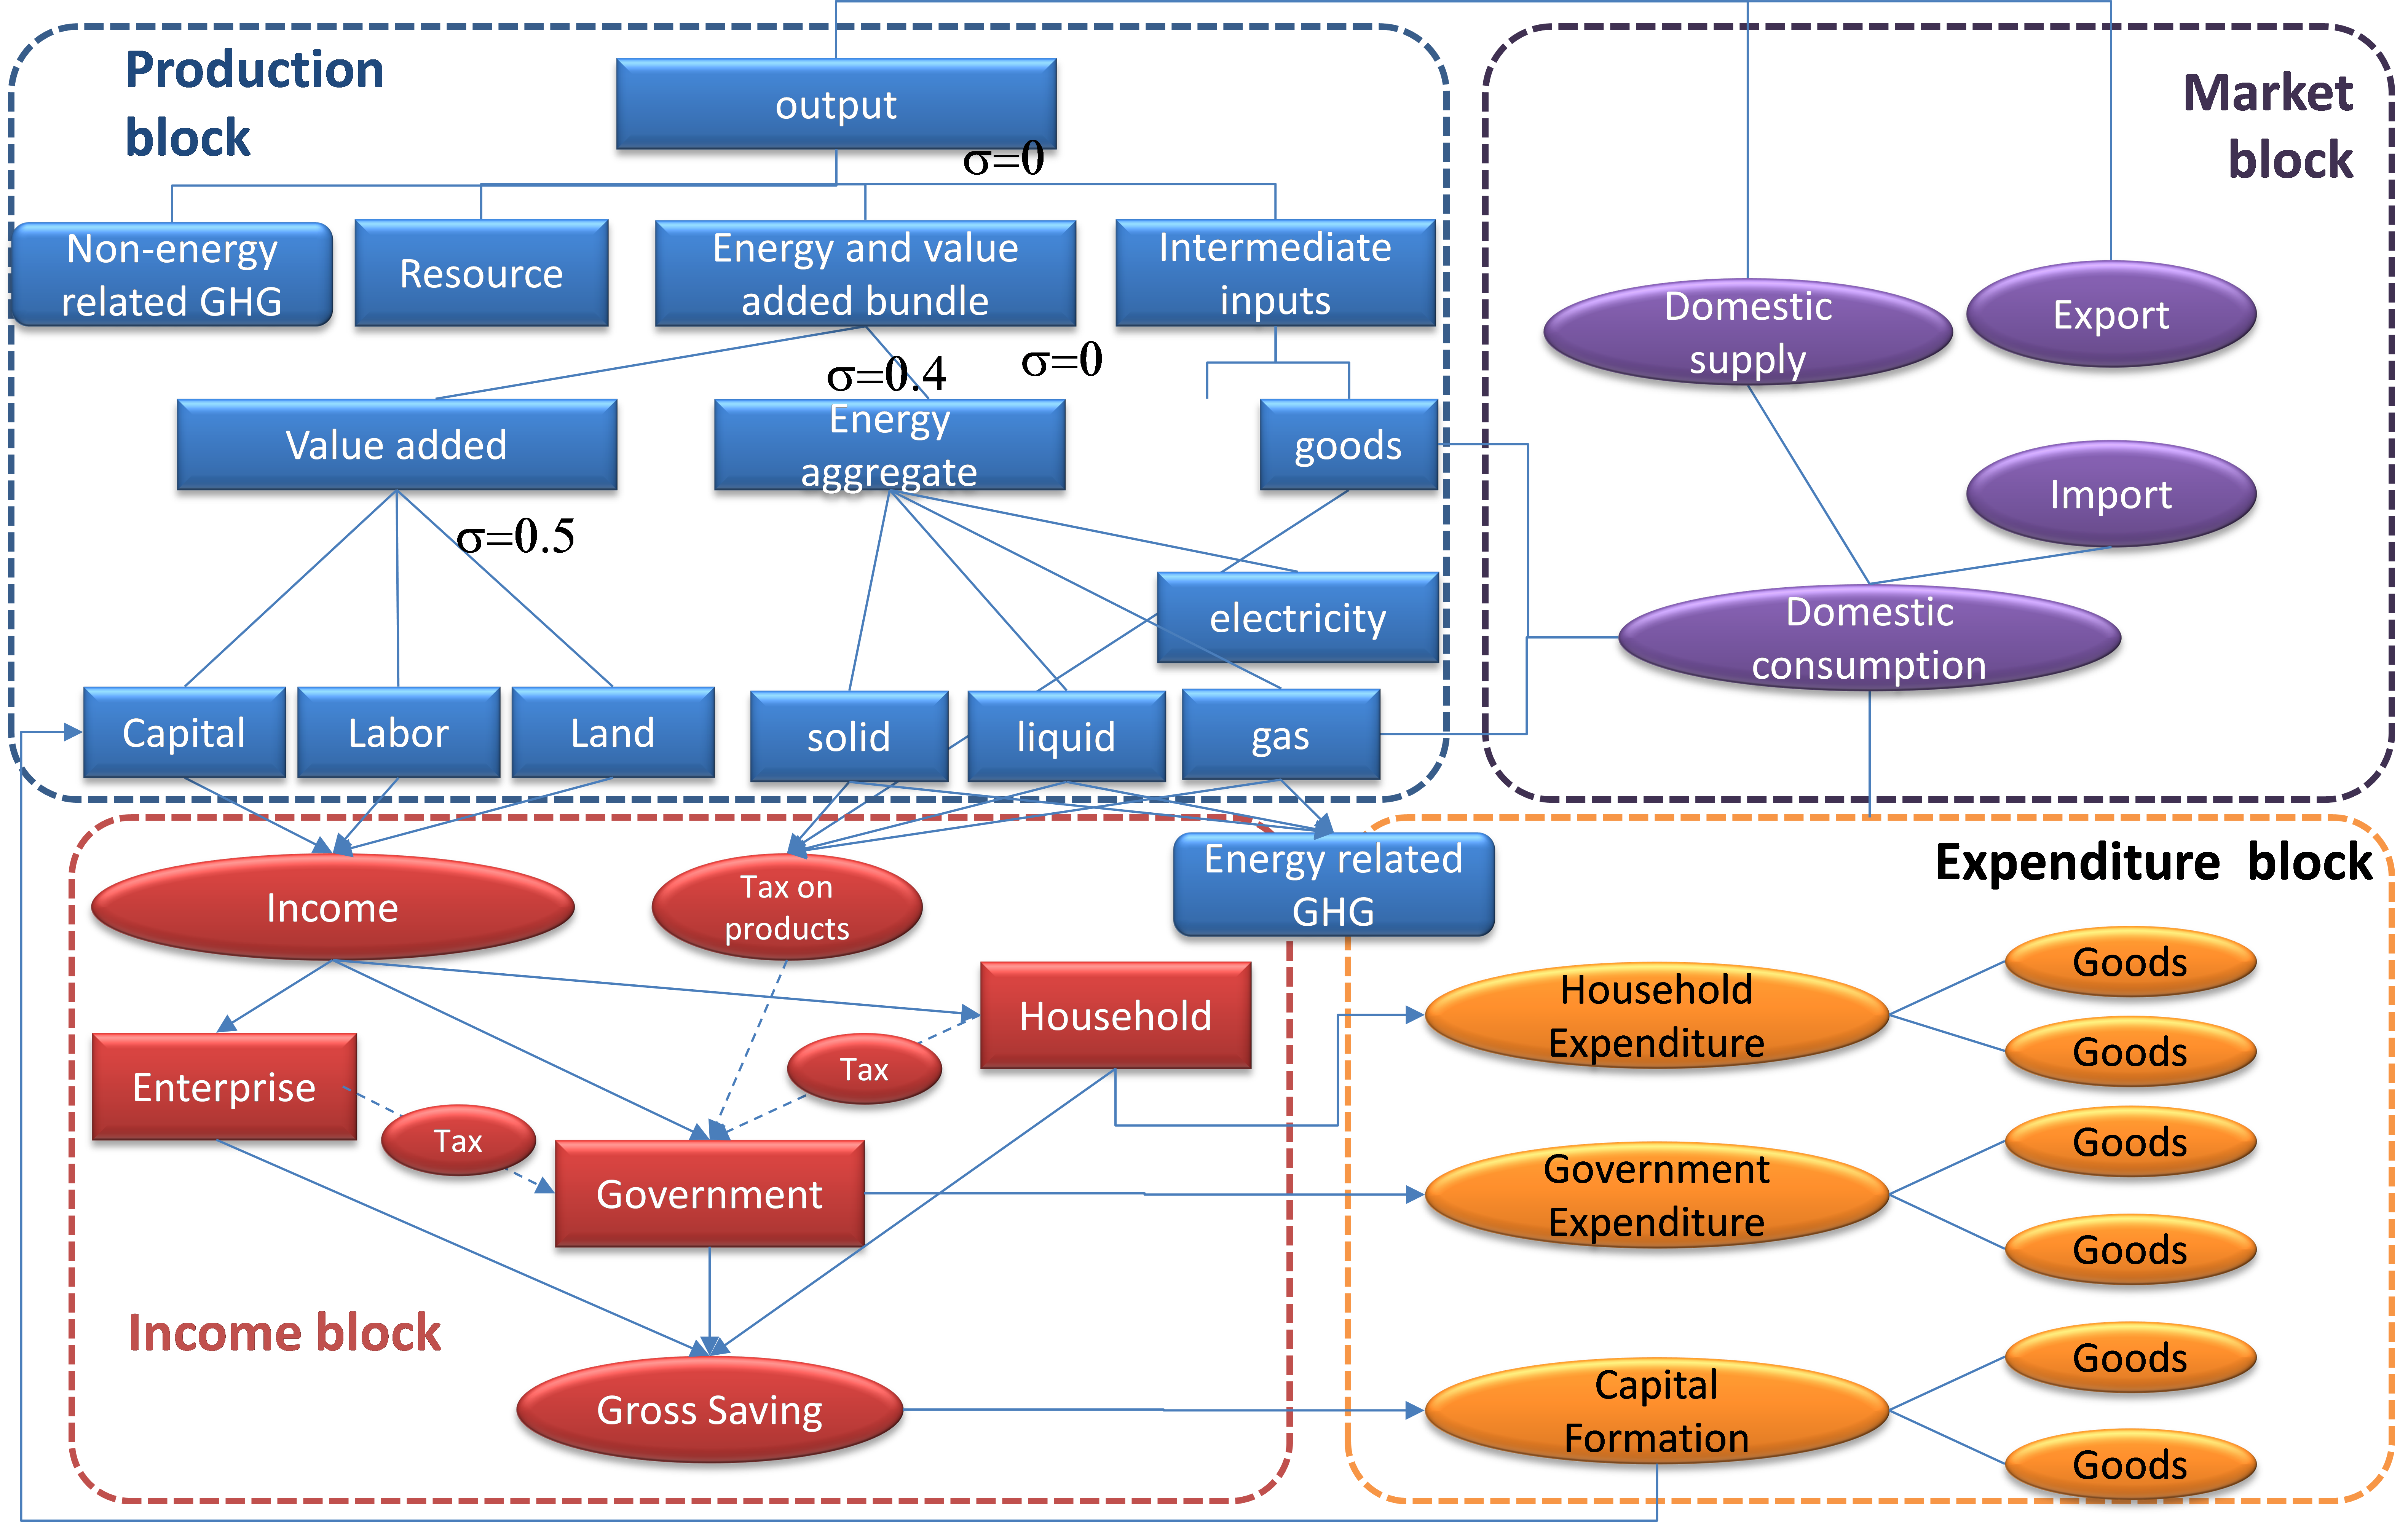
\includegraphics[width=1\textwidth]{fig/image2.png} 
\caption{\label{fig:overview} Overview of AIM/Hub model structure}
\end{figure}

There are four blocks: production, income distribution, final consumption, and market. The first block, production, represents the structure of the production functions. We apply a nested CES function for production activities with multiple nested CES functions. Secondly, incomes are distributed to three institutional sectors: enterprises, government, and households. The government takes in income by collecting taxes. Thirdly, institutions consume goods as final consumption. Government expenditure and capital formation are defined as a constant coefficient function. The LES (Linear Expenditure System) or AIDADS (An Impricit Direct Additive Demand System) is used for household consumption. Lastly, the CES function is applied to the import of goods and the CET function is applied to the export of goods. A goods-consumption-and-supply equilibrium is achieved for each market.

\section{\label{sec:ActProdFac}Activity production and factor markets}

Each producer (represented by an activity) is assumed to maximize profits, defined as the difference between revenue earned and the cost of factors and intermediate inputs. Profits are maximized subject to a production technology, the structure of which is shown in Figure \ref{fig:ProductionStructure}. At the top level, there is non-energy related GHG emission and conventional inputs. This GHG emission treatment is described in detailed by Hyman~\cite{RN2134}. Conventional inputs technology is specified by a Leontief function of the quantities of energy and value-added bundle, aggregate non-energy intermediate input and resource input. Energy and value added bundle is nested by valued added and energy inputs. Value added is itself a constant elasticity of substitution (CES) function of primary factors. The aggregated energy inputs are specified by a Logit function. The aggregate intermediate input is a Leontief function of disaggregated intermediate inputs. 
\begin{figure}
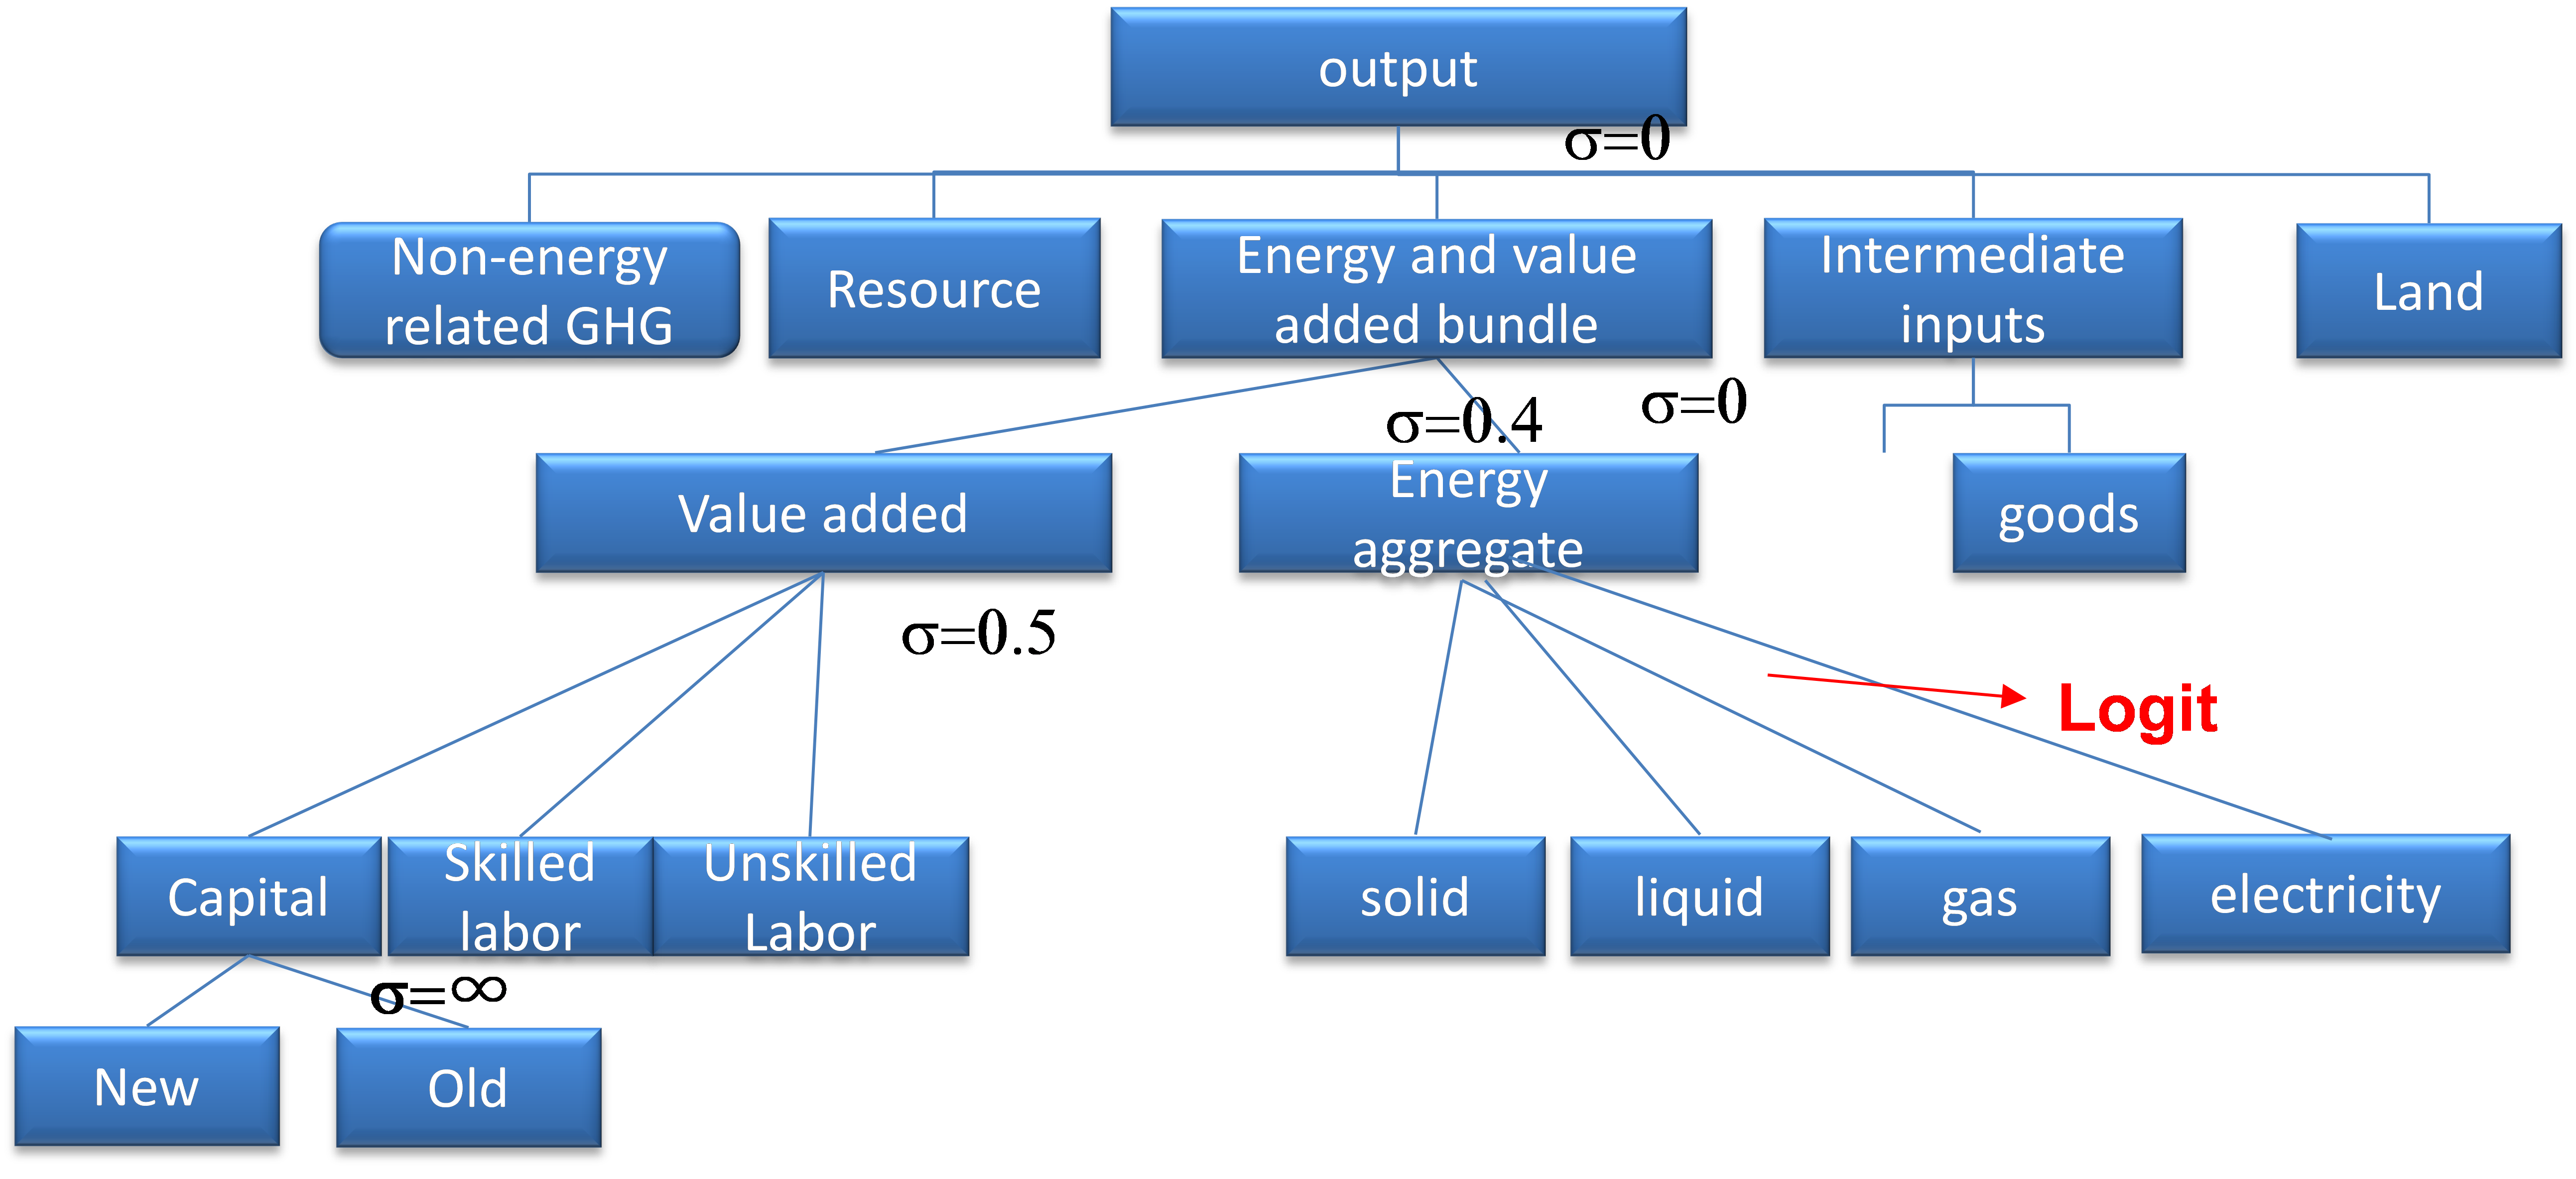
\includegraphics[width=1\textwidth]{fig/image3.png}
\caption{\label{fig:ProductionStructure} Production structure (Non-energy transformation sectors)}   
\label{fig:2}
\end{figure}
The energy transformation sectors such as the power and petroleum refinery sectors are assumed to be different production functions from the other sectors. The structure is drawn as below. Value added aggregation and energy inputs are speficied by Leontief.

There is an option to specify the each sector's energy consumption by using detailed enduse technology device information. Once the option turned on, the energy consumption is separated from value added nest and determined by device selection Logit function and the devices input energy sources.
\begin{figure}
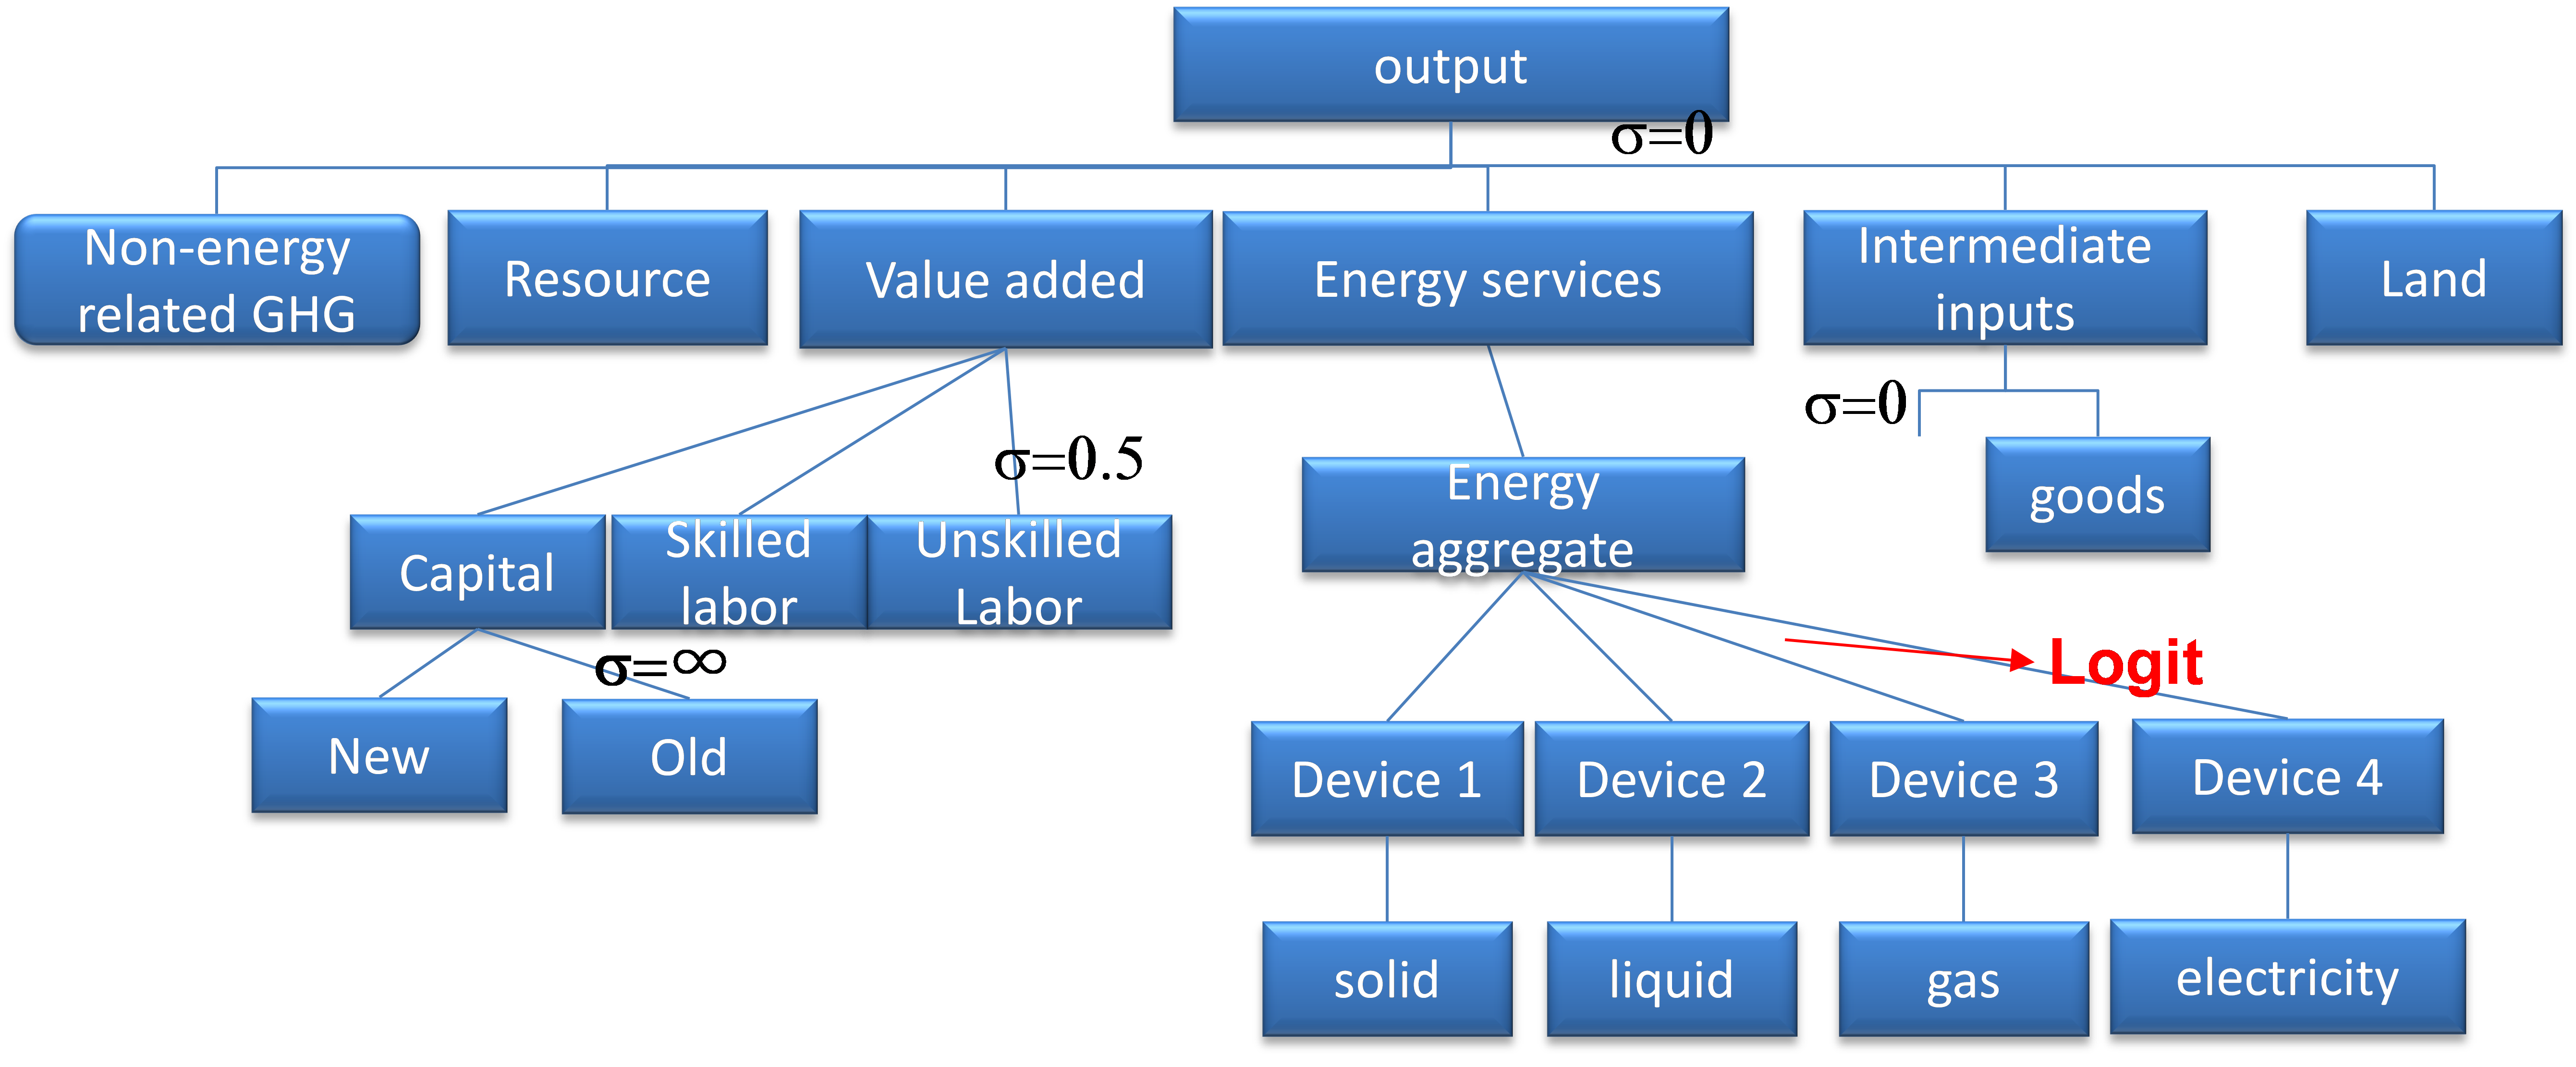
\includegraphics[width=1\textwidth]{fig/image4.png}
\caption{\label{fig:Production structure2}Production structure (Non-energy transformation sectors) with enduse option}
\end{figure}

\begin{figure}
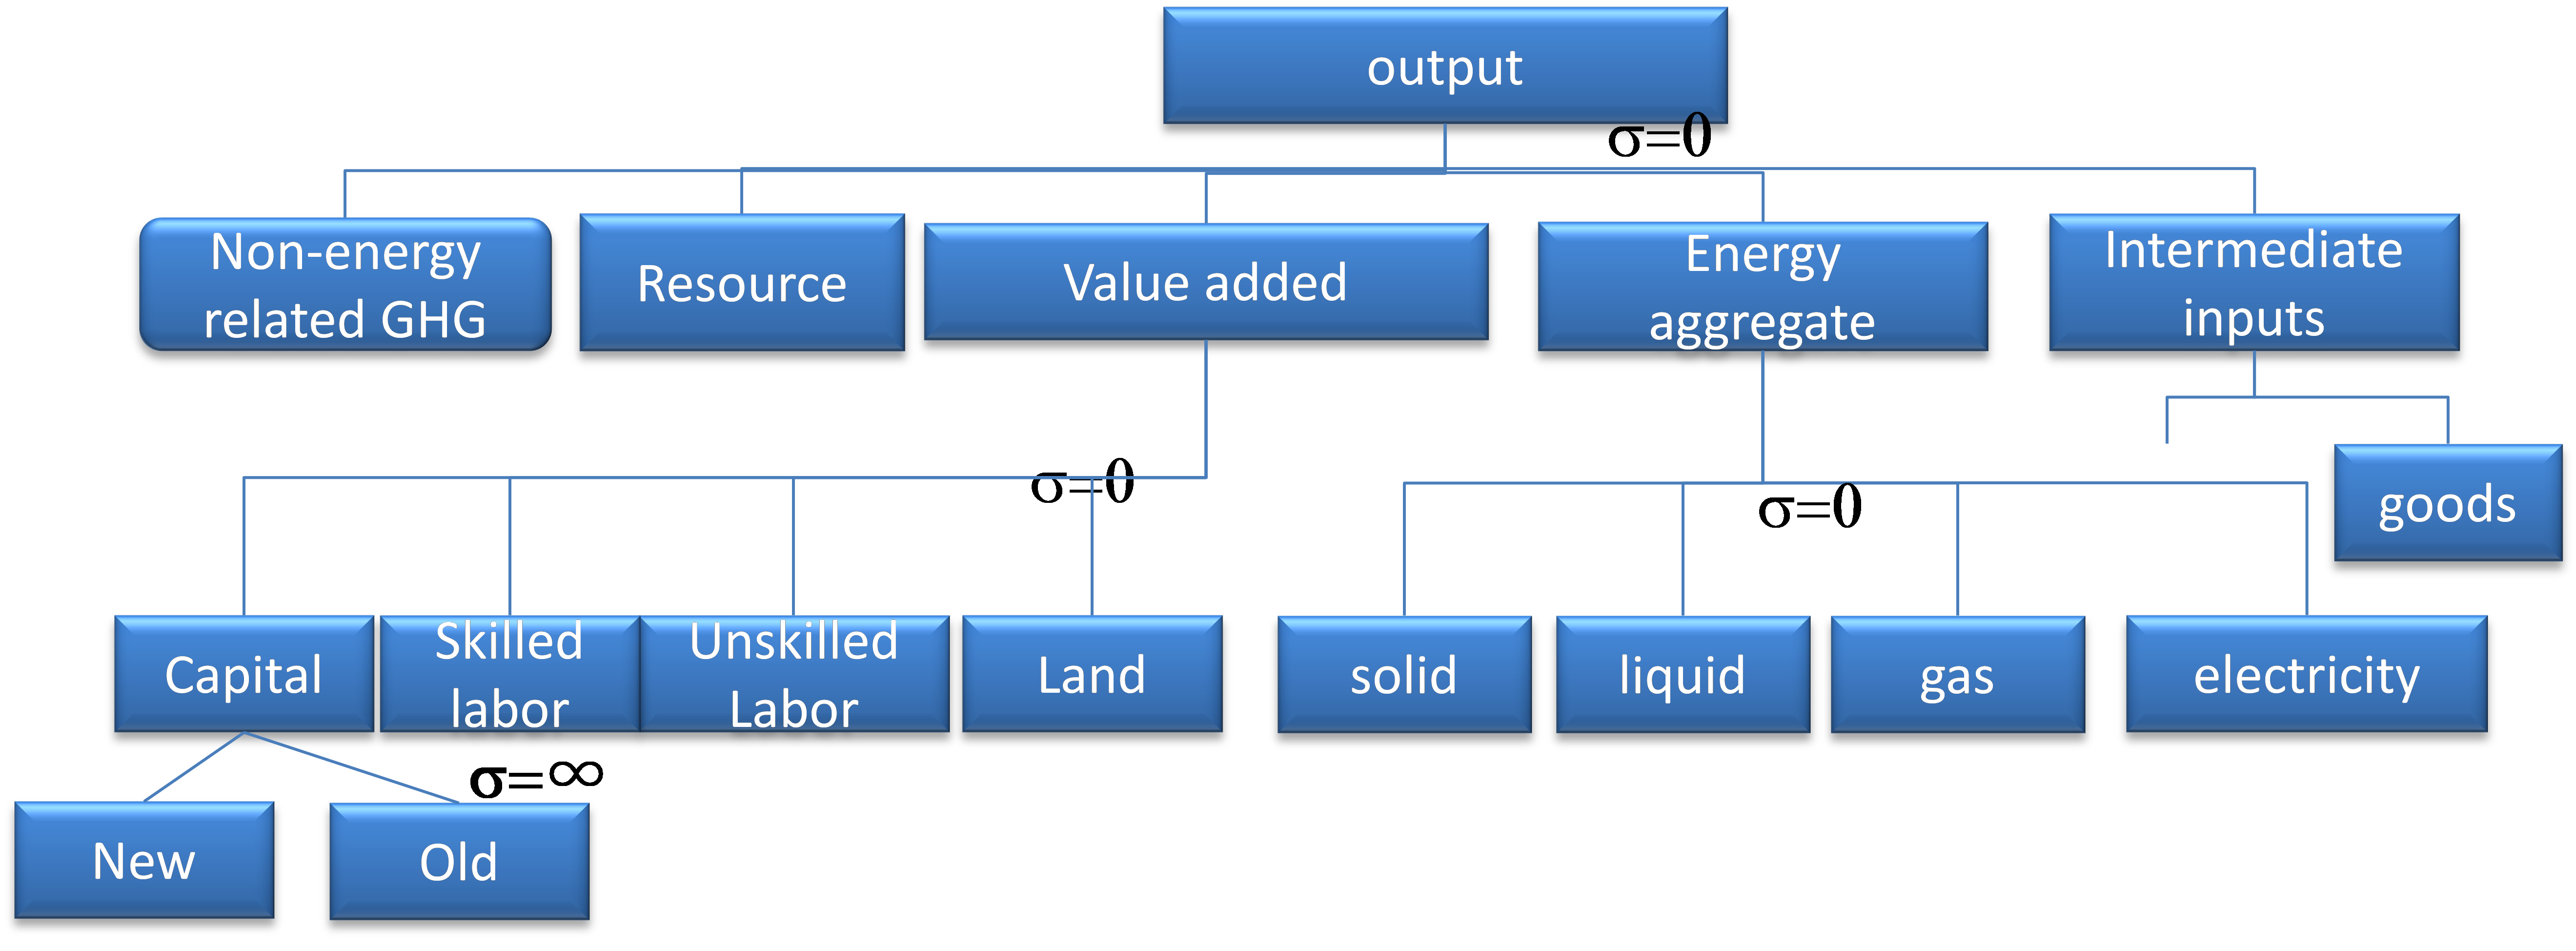
\includegraphics[width=1\textwidth]{fig/image5.png}
\caption{\label{fig:Production structure 3}Production structure (Energy transformation sectors)} 
\end{figure}
Each activity produces one or more commodities according to fixed yield coefficients. A commodity may be produced by more than one activity. In this model, the electricity is produced by many types of power supply technology. The revenue of the activity is defined by the level of the activity, yields, and commodity prices at the producer level. 

As part of its profit-maximizing decision, each activity uses a set of factors up to the point where the marginal revenue product of each factor is equal to its factor price. The quantity supplied of each factor is fixed at a certain level. As for the captital, the capital accumulation is taken into account. This level is recursive dynamically decided. An economy-wide wage variable is free to vary to assure that the sum of demands from all activities equals the quantity supplied. New capital is allocated to anywhere. Old capital is assumed to be fixed to each sector, which is named the putty-clay assumption. The rate of return of capital is same for both of old and new capitals. However, if the new capital is not allocated, the price of old capital is lower than new one and the operation ratio could be lower than 1. 

\section{\label{sec:Inst}Institutions}

In the CGE model, institutions are represented by: households, enterprises, the government, and the rest of the world\footnote{This is the default version classification but if the long-term simulation like till 2100 is the objectives, household government and enterprises are treated as one aggregated representative household. }. The households (disaggregated as in the SAM) receive income from the factors of production (directly or indirectly via the enterprises) and transfers from other institutions. The households use their income to pay direct taxes, save, consume, and make transfers to other institutions. In the basic model version, direct taxes and transfers to other domestic institutions are defined as fixed shares of household income whereas the savings share is flexible for selected households. The income that remains after taxes, savings, and transfers to other institutions is spent on consumption. When the economy has to implement carbon tax, all of the revenues are assumed to be receipt by the household.

Household consumption covers marketed commodities, purchased at market prices that include commodity taxes. Household consumption is allocated across different commodities according to linear expenditure system (LES) demand functions, derived from maximization of a Stone-Geary utility function.

Instead of being paid directly to the households, factor incomes may be paid to the enterprise. The Enterprise may also receive transfers from other institutions. Enterprise incomes are allocated to direct taxes, savings, and transfers to other institutions. Enterprises do not consume. Apart from this, the payments to and from enterprises are modeled in the same way as the payments to and from households. The government collects taxes and receives transfers from other institutions. In the basic model version, all taxes are at fixed \textit{ad valorem} rates. 

The government uses this income to purchase commodities for its consumption and for transfers to other institutions. Government consumption is fixed in real (quantity) terms whereas government transfers to domestic institutions (households and enterprises) are CPI-indexed. Government savings (the difference between government income and spending) is a flexible residual. 

The saving rate made by all institution is fixed coefficient also.

The final institution is the rest of the world. As noted, transfer payments between the rest of the world and domestic institutions and factors are all fixed in foreign currency. Foreign savings (or the current account deficit) is the difference between foreign currency spending and receipts. Commodity trade with the rest of the world is discussed in the next section. 

\section{\label{sec:ComMar}Commodity market}

All commodities (domestic output and imports) enter markets. Domestic output may be sold in the market. For marketed output, the first stage in the chain consists of generating aggregated domestic output from the output of different activities of a given commodity. These outputs are imperfectly substitutable as a result of, for example, differences in timing, quality, and distance between the locations of activities. A CES function is used as the aggregation function\footnote{Energy commodity has specific treatment. It is discussed below}. The demand for the output of each activity is derived from the problem of minimizing the cost of supplying a given quantity of aggregated output subject to this CES function. Activity-specific commodity prices serve to clear the implicit market for each disaggregated commodity. 

In the next, aggregated domestic output is allocated between exports and domestic sales on the assumption that suppliers maximize sales revenue for any given aggregate output level, subject to imperfect transformability between exports and domestic sales, expressed by a constant elasticity of transformation (CET) function. In the international markets, export demands are infinitely elastic at given world prices. The price received by domestic suppliers for exports is expressed in domestic currency and adjusted for export taxes (if any). If the commodity is not exported, total output is passed to the domestic market.

Domestic demand is made up of the sum of demands for household consumption, government consumption, investment (the determination of which is discussed below), and intermediate inputs.

To the extent that a commodity is imported, all domestic market demands are for a composite commodity made up of imports and domestic output, the demands for which are derived on the assumption that domestic demanders minimize cost subject to imperfect substitutability. This is also captured by a CES aggregation function which is so-called Armington assumption. Total market demand is directed to imports for commodities that lack domestic production and to domestic output for non-imported commodities. The derived demands for imported commodities are met by international supplies that are infinitely elastic at given world prices. The import prices paid by domestic demanders also include import tariffs (at fixed \textit{ad valorem} rates) and the cost of a fixed quantity of transactions services per import unit, covering the cost of moving the commodity from the border to the demander. Similarly, the derived demand for domestic output is met by domestic suppliers. 

The AIM/HUB model treats the volume of energy commodities\footnote{Coal (COA), crude oil (OIL), natural gas (GAS), petroleum products (P\_C), town gas (GDT) and electricity (ELY)} as energy units, though usual CGE model do not as well. In the calibration procedure, the energy unit transaction data is used.

Although energy commodities must satisfy the energy balance condition, CES and CET function make the balanced condition. Therefore, we apply specific formulas to the energy and agricultural commodities that are treated as physical volume, which is a sort of Logit function. We determine the share of imported and domestic consumption by the ratio of the current price to previous year's price. The share of exported and domestic consumption, and the share of the same commodity production are determined as well as the import composition. The share is controlled by the ratio of previous year's and calculation year price with an elasticity parameter. For example, if import price is increased over that of domestic products, the share of import commodity would be decreased.

\section{\label{sec:LanAlloMar}Land allocation and its market}

Land is disaggregated into AEZ (Agro-Ecological Zone) categories, and default version assumes 3 kinds of land type (AEZ1 to AEZ3). The land use sectors; cropping, livestock and forestry, input these land categories. The farmers and forestry activities determine the share of the land input according to the land price. 

On the other hand, the land owners decide the share of land use according to the land price and there are multiple decisions to allocate the land to each activity. Firstly, agricutlrue and forestry land are identified. Then, forestry is disaggregated into primary and secondary forestry. The other blanch has grass land and crop land disaggregation. Grass land has unused primary area and grazing area. Crop land and grazing area have final disaggregation to each specific commodity production activity. Each decision is based on Logit function. This decision process is illustrated in Figure \ref{fig:LandAll}.
\begin{figure}
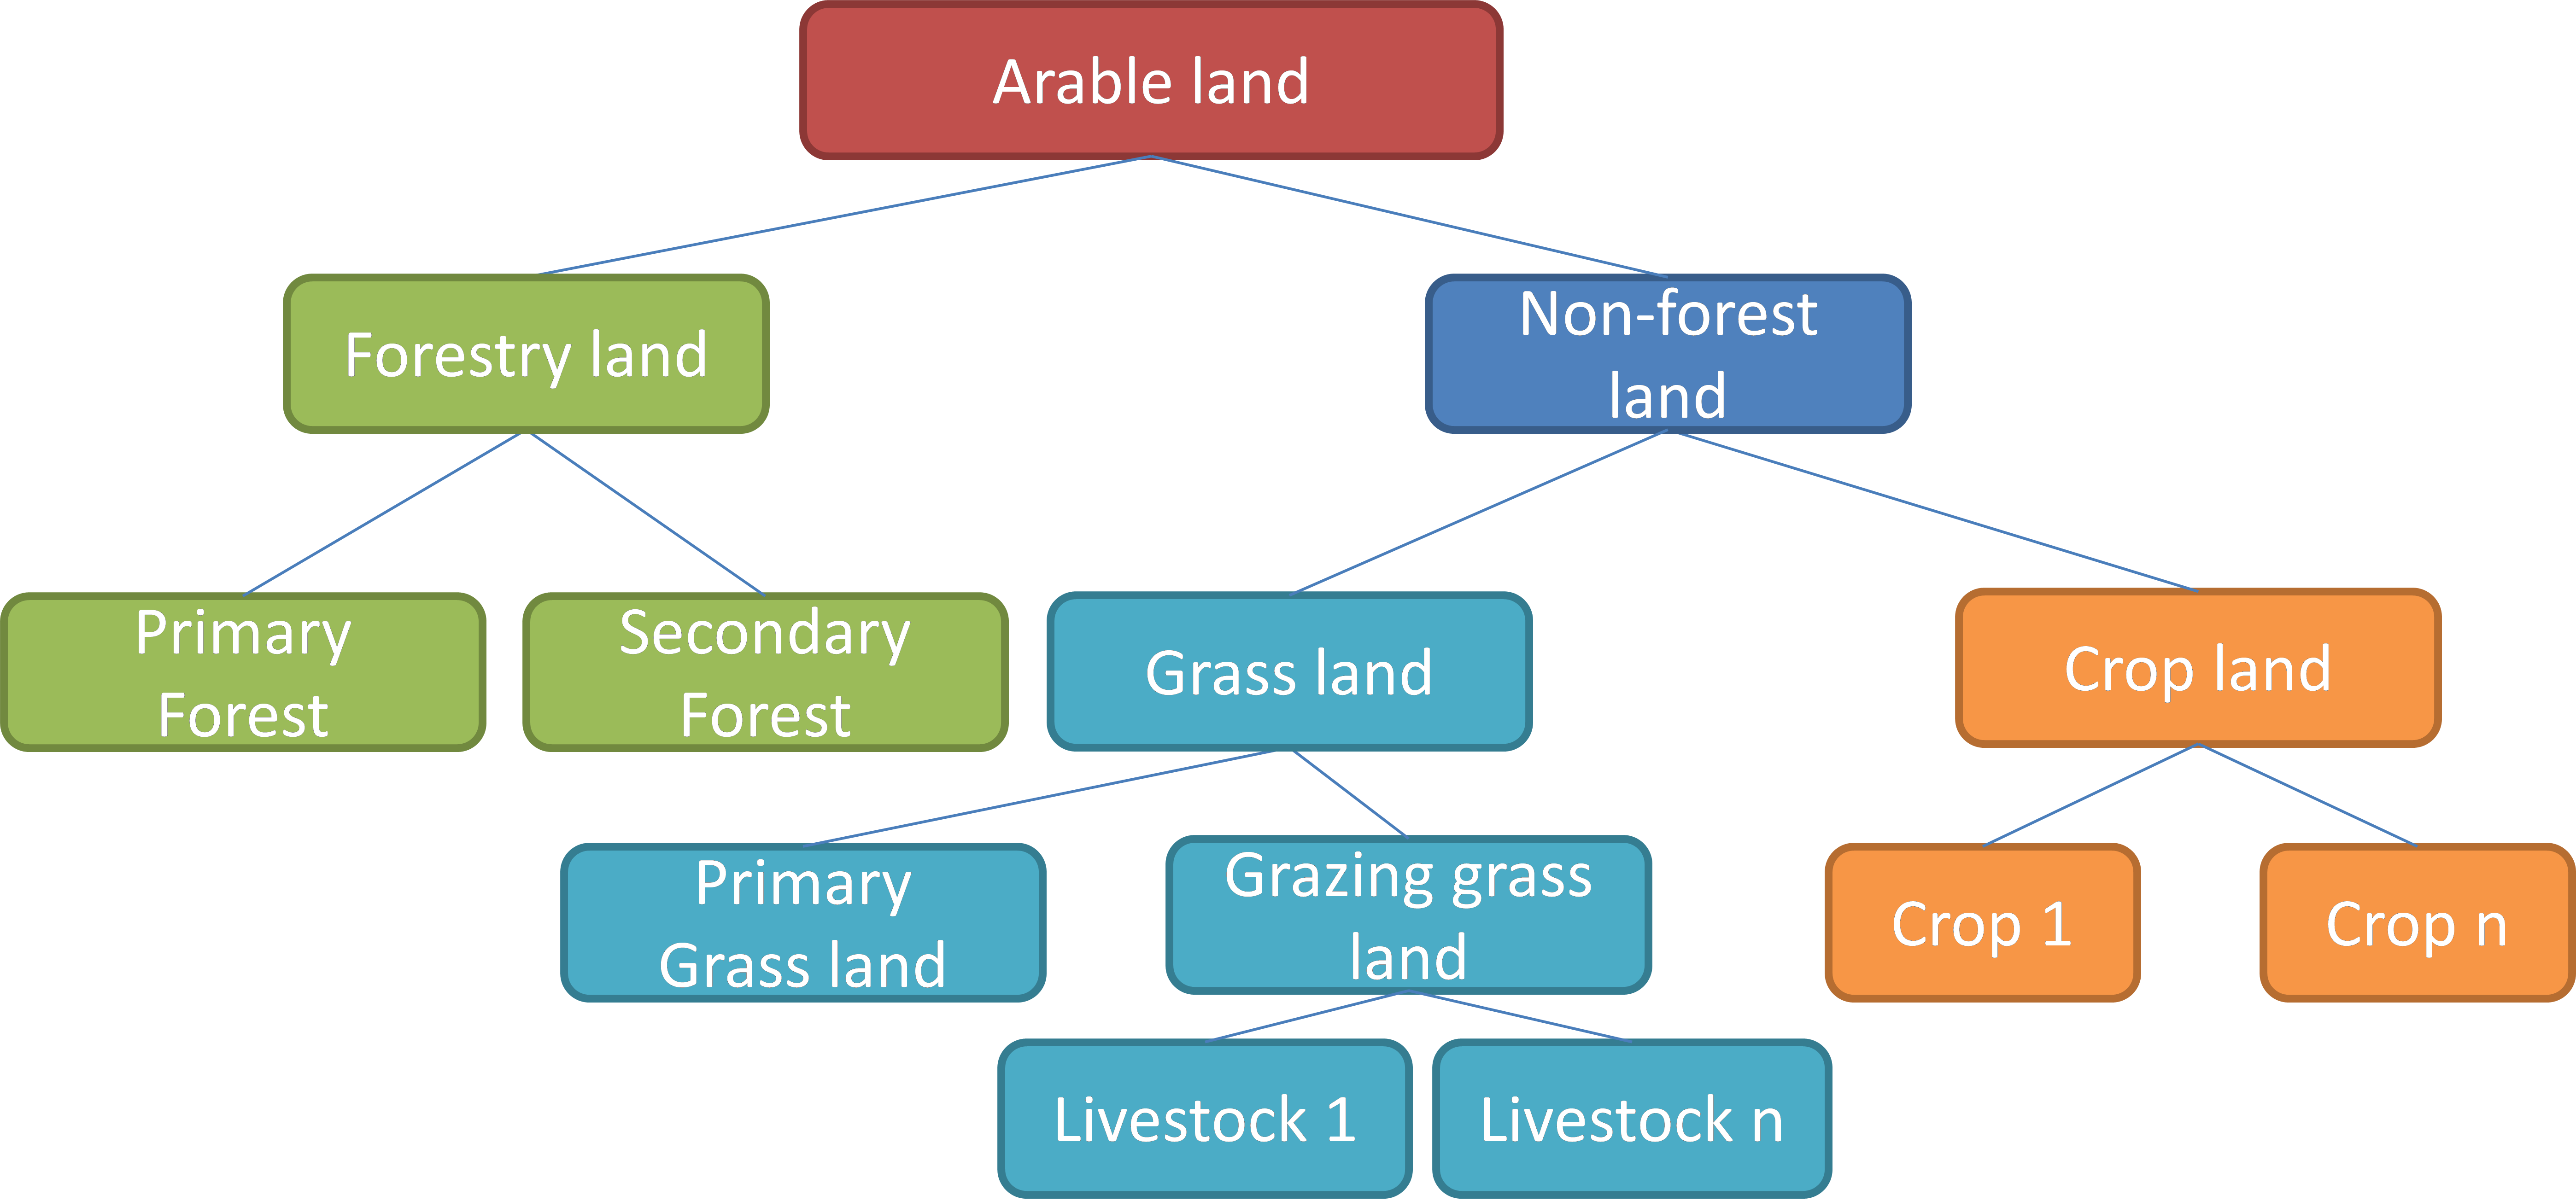
\includegraphics[width=1\textwidth]{fig/image6.png}
\caption{\label{fig:LandAll}Land allocation strucuture}
\end{figure}

\section{\label{sec:MacEcoBala}Macro economic balances}

The CGE model includes three macroeconomic balances: the (current) government balance, the external balance (the current account of the balance of payments, which includes the trade balance), and the Savings-Investment balance.

For the government balance, the closure is that government savings (the difference between current government revenues and current government expenditures) is a flexible residual while all tax rates are fixed. 

For the external balance, which is expressed in foreign currency, the closure is that the real exchange rate is flexible while foreign savings (the current account deficit) is fixed. Given that all other items are fixed in the external balance (transfers between the rest of the world and domestic institutions), the trade balance is also fixed. 

For the Savings-Investment balance, the closure is investment-driven. Real investment quantities are fixed. In order to generate savings that equal the cost of the investment bundle, the base-year savings rates of selected nongovernment institutions are adjusted by the same number of percentage points. Implicitly, it is assumed that the government is able to implement policies that generate the necessary private savings to finance the fixed real investment quantities.

\section{\label{sec:Stru-AirPolGHGEmi}Air pollutants and GHG emissions}

The CGE model includes air pollutants and GHG emissions module. The emission gases treated in this model are CO, NH\textsubscript{3}, NMVOC, NOx, SO\textsubscript{2}, BC, OC, CO\textsubscript{2} CH\textsubscript{4} and N\textsubscript{2}O. The emission sources are classified into two groups; (1) One is related to fuel combustion and this kind of emission is proportional to the energy consumption. (2) The other is related to the activity level, e.g. CO\textsubscript{2} emission from cement production, and this kind of emission is proportional to the activity level. The emission sources and their groups are shown in Table \ref{tab:EmissionSources}. There are other categories that are not classified in IPCC but exist in the model in Table \ref{tab:Non-IPCC}.


\begin{tabularx}{\textwidth}{ll} 
\caption{\label{tab:EmissionSources} Emission sources}
\\\hline 
IPCC category & Explanation \\\hline 
1A1a & Public electricity and heat production\\
1A1bc & Other Energy Industries\\
1A2 & Manufacturing Industries and Construction\\
1A3a & Domestic aviation\\
1A3b & Road transportation\\
1A3c & Rail transportation\\
1A3d & Inland navigation\\
1A3e & Other transportation\\
1A4 & Residential and other sectors\\ \hline 
2A & Production of minerals\\
2A1 & Cement production\\
2A2 & Lime production\\
2B & Production of chemicals\\
2C & Production of metals\\
2D & Production of pulp/paper/food/drink\\
2G & Non-energy use of lubricants/waxes (CO2)\\
3A & Solvent and other product use: paint\\
3B & Solvent and other product use: degrease\\
3C & Solvent and other product use: chemicals\\
3D & Solvent and other product use: other\\
4A & Enteric fermentation\\
4B & Manure management\\
4C & Rice cultivation\\
4D1 & Direct soil emissions\\
4D2 & Manure in pasture/range/paddock\\
4D3 & Indirect N2O from agriculture\\
4D4 & Other direct soil emissions\\
4E & Savanna burning\\
4F & Agricultural waste burning\\
5A & Forest fires\\
5C & Grassland fires\\
5F2 & Forest Fires-Post burn decay\\
6A & Solid waste disposal on land\\
6B & Wastewater handling\\
6C & Waste incineration\\
6D & Other waste handling\\ \hline 
\end{tabularx}

\begin{tabularx}{\textwidth}{ll} 
\caption{\label{tab:Non-IPCC} Emission sources for non-IPCC categories}
\\\hline 
Code & Description \\\hline
 5X & Other land use change \\ 
 5Y & Carbon sink in land  \\ 
 5Z & Wood removal \\ 
 10X & CCS removal \\ 
 10Y & Biomass emissions (But net accounted as zero) \\ \hline 
\end{tabularx}

\chapter{\label{chp:Math}Mathematical statement}

This chapter presents the mathematical model statement equation by equation. In its mathematical form, the CGE model is a system of simultaneous, nonlinear equations. The model is square - that is, the number of equations is equal to the number of variables. In this class of models, this is a necessary (but not a sufficient) condition for the existence of a unique solution. The chapter divides the equations into six blocks: prices, production and trade, institutions, international trade\footnote{The equations in the ''International trade block'' are involved only if you chose a global model.}, energy and CO\textsubscript{2} emissions, and system constraints. New items (sets, parameters, and variables) are defined the first time that they appear in the equations. Table \ref{tab:Notation} summarizes the notational principles. Parameter and variable names are chosen to facilitate interpretation; most importantly, commodity and factor quantities start with \textit{q}, commodity prices with \textit{p}, and factor prices with \textit{w}.

%\begin{tabularx}{\textwidth}{|
%p{\dimexpr 0.3\linewidth-2\tabcolsep-2\arrayrulewidth}|
%p{\dimexpr 0.6\linewidth-2\tabcolsep-\arrayrulewidth}|}
\begin{tabularx}{\linewidth}{|X|X|}
\caption{\label{tab:Notation}Notational principles}
\\\hline 
Item & Notation \\\hline
Endogenous variables & Upper-case Latin letters without a bar \\
Exogenous variables & Upper-case Latin letters with a bar \\
Paramters & Lower-case Latin letters (with or without a bar) or lower-case Greek letters (with or without superscripts) \\
Set indices & Lower-case Latin letters as subscripts to variables and parameters \\\hline
\end{tabularx}


 The price system of the model is rich, primarily because of the assumed quality differences among commodities of different origins and destinations (exports, imports, and domestic outputs used domestically). The price block consists of equations in which endogenous model prices are linked to other prices (endogenous or exogenous) and to non-price model variables.

\begin{flushleft}\textbf{Import Price }\end{flushleft}

\begin{center}$PM_{r,c}=PWMR_{r,c}\cdot \left(1+tm_{r,c}\right)\cdot \overline{EXR_{r}},\,\,\,\,\forall r\in R,\,c\in CM$ (PMEDEF)
\end{center}

\begin{flushleft}
$r\in R$: a set of regions,

$c\in C$: a set of commodities (also referred to as \textit{c'} and \textit{C'}),

$c\in CM\left(\subset C\right)$: a set of imported commodities,

$PM_{r,c}$: composite commodity price (including import tax and transaction costs),

$PWMR_{r,c}$: Import price of commodity \textit{c} in region \textit{r,}

$tm_{r,c}$: import tariff rate,

$EXR_{r}$: exchange rate country \textit{r.}
\end{flushleft}

The import price is the price paid by domestic users for imported commodities (exclusive of the sales tax). Equation (PMDEF) states that it is a transformation of the world price of these imports, considering the exchange rate and import tariffs plus transaction costs (the cost of trade inputs needed to move the commodity from the border to the demander) per unit of the import. The domain of the equation is the set of imported commodities (a subset of the commodity set). The model includes one equation like (PMDEF) for every imported commodity.

Note that the notational principles make it possible to distinguish between variables (upper-case Latin letters) and parameters (lower-case Latin letters). This means that the exchange rate and the domestic import price are flexible, while the tariff rate and the world import price are fixed. The fixedness of the world import price stems from the ''small-country'' assumption. That is, for all its imports, the assumed share of world trade for the modeled country is so small that it faces an infinitely elastic supply curve at the prevailing world price.

\begin{flushleft}\textbf{Export Price}\end{flushleft}


\begin{center}$PE_{r,c}=PWER_{r,c}\cdot \left(1-te_{r,c}\right)\cdot \overline{EXR_{r}},\,\,\,\,\forall r\in R,\,c\in CE$ (PEDEF)
\end{center}
\begin{flushleft}
$c\in CE\left(\subset C\right)$: a set of exported commodities (with domestic production),

$PE_{r,c}$: export price of commodity \textit{c,}

$PWMR_{r,c}$: Export price of commodity \textit{c} in region \textit{r,}

$te_{r,c}$: export tax rate.
\end{flushleft}

The export price is the price received by domestic producers when they sell their output in export markets. This equation is similar in structure to the import price definition. The main difference is that the tax reduces the price received by the domestic producers of exports (instead of adding to the price paid by domestic demanders of imports). The domain of the equation is the set of exported commodities, all of which are produced domestically.

\begin{flushleft}\textbf{Demand Price of Domestic Non-traded Goods}\end{flushleft}


\begin{center}$PDD_{r,c}=PDS_{r,c},\,\,\,\,\forall r\in R,\,c\in CD$ (PDDDEF)
\end{center}

\begin{flushleft}
$c\in CD\left(\subset C\right)$: a set of commodities with domestic sales of domestic output,

$PDD_{r,c}$: demand price for commodity produced and sold domestically,

$PDS_{r,c}$: supply price for commodity produced and sold domestically. 
\end{flushleft}

Equation (PDDDEF) defines the demand prices as the supply price.

\begin{flushleft}\textbf{Absorption}\end{flushleft}


\begin{center}$PQ_{r,c}\cdot QQ_{r,c}=PDD_{r,c}\cdot QD_{r,c}+PM_{r,c}\cdot QM_{r,c},\,\,\,\,\forall r\in R,\,c\in \left(CD\cup CM\right)$ (PQDDEF)
\end{center}
\begin{flushleft}
$PQ_{r,c}$: composite commodity price excluding sales tax,

$QQ_{r,c}$: quantity of goods supplied to domestic market (composite supply),

$QD_{r,c}$: quantity sold domestically of domestic output,

$QM_{r,c}$: quantity of imports of commodity.
\end{flushleft}

Absorption is total domestic spending on a commodity at domestic demander prices. Equation (PQDDEF) defines it exclusive of the sales tax. Absorption is expressed as the sum of spending on domestic output and imports at the demand prices, \textit{PDD} and \textit{PM}. The prices \textit{PDD} and \textit{PM} include the cost of trade inputs but exclude the commodity sales tax.

The equation as a whole applies to all commodities that are imported and/or have domestic sales of domestic output (the union of the sets \textit{CD} and \textit{CM}). It does not apply to commodities for which the entire output volume is exported. Each of the two terms on the right-hand side applies only to its relevant set (\textit{CD} and \textit{CM}, respectively). In the \textit{GAMS} code, \textit{PM} and \textit{QM} are fixed at zero for commodities that are not elements in the set \textit{CM}; similarly \textit{PDD} and \textit{QD} are fixed at zero for commodities that are not elements in the set \textit{CD}. This approach is followed throughout: all variables that should be excluded from the model are fixed at zero. 

\begin{flushleft}\textbf{Commodity market monetary balance}\end{flushleft}


\begin{center}$PQ_{r,c}\cdot QQ_{r,c}=PQD_{r,c}\cdot \left(\begin{array}{cc} & \sum _{a\in A}dfpq_{r,c,a}\cdot QINT_{r,c,a}+\sum _{h\in H}pfdq_{r,c,h}\cdot QH_{r,c,h}\\ & +pfdq_{r,c,"gov"}\cdot QG_{r,c}+pfdq_{r,c,"S-I"}\cdot QINV_{r,c}
\end{array}\right),\,\,\,\,\forall r\in R,\,c\in CX$ (PQDEF)
\end{center}

\begin{flushleft}
$PQD_{r,c}$: composite commodity price excluding sales tax,

$dfpq_{r,c,i}$: price differences of commodity price among inputs sectors,

$QINT_{r,c,a}$: quantity of commodity \textit{c} as intermediate input to activity \textit{a},

$QH_{r,c,h}$: quantity of consumption of marketed commodity \textit{c} for household \textit{h,}

$QG_{r,c}$: government consumption demand for commodity,

$QINV_{r,c}$: quantity of fixed investment demand for commodity.
\end{flushleft}

\begin{flushleft}\textbf{Marketed Output with stock change}\end{flushleft}


\begin{center}$QX2_{r,c}=QX_{r,c}+stch_{r,c},\,\,\,\,\forall r\in R,\,c\in CX$ (QX2DEF)
\end{center}

\begin{flushleft}
$QX_{r,c}$: aggregate marketed quantity of domestic output of commodity,

$QX2_{r,c}$: aggregate marketed quantity of domestic output of commodity including stock change,

$stch_{r,c}$: stock change of commodity \textit{c} (positive).
\end{flushleft}

\begin{flushleft}\textbf{Marketed Output Value with stock change}\end{flushleft}


\begin{center}$PX2_{r,c}\cdot QX2_{r,c}=PX_{r,c}\cdot QX_{r,c},\,\,\,\,\forall r\in R,\,c\in CX$ (PXDEF)
\end{center}

\begin{flushleft}
$PX_{r,c}$: aggregate producer price for commodity,

$PX2_{r,c}$: aggregate producer price for commodity including stock change effects.
\end{flushleft}

The above 2 equations describe the relataionship between output and stock changes, and those of market value.

\begin{flushleft}\textbf{Marketed Output Value}\end{flushleft}


\begin{center}$PX2_{r,c}\cdot QX2_{r,c}=PDS_{r,c}\cdot QD_{r,c}+PE_{r,c}\cdot QE_{r,c},\,\,\,\,\forall r\in R,\,c\in CX$ (PX2DEF)
\end{center}

\begin{flushleft}
$c\in CX\left(\subset C\right)$: a set of commodities with domestic output,

$QE_{r,c}$: quantity of exports.
\end{flushleft}
For each domestically produced commodity, the marketed output value at producer prices is stated as the sum of the values of domestic sales and exports. Domestic sales and exports are valued at the prices received by the suppliers, \textit{PDS} and \textit{PE}, both of which have been adjusted downwards to account for the cost of trade inputs. 

The domain limitation to domestically produced commodities (the elements in the set \textit{CX}) has to be stated explicitly given that the model includes a category of imported commodities without domestic production. The domestic part applies only to elements in \textit{CD} whereas the export part applies only to elements in \textit{CE}. \textit{PX} and \textit{QX} are referred to as ''aggregate'' values since they may apply to an aggregation of output from different domestic producers of the same commodity. By dividing through by \textit{QX2}, this equation could be rewritten as an explicit definition of \textit{PX}.

\begin{flushleft}\textbf{Consumer Price Index}\end{flushleft}


\begin{center}$CPI_{r}=\sum _{c\in C}\left(PQD_{r,c}\cdot dfpq_{r,c,"hurb"}\cdot \left(1+tqd_{r,c,"hurb"}\right)\right)\cdot cwts_{r,c}\,\,\forall r\in R,\forall g\in G$ (CPIDEF)
\end{center}

\begin{flushleft}
$cwts_{r,c}$: weight of commodity c in the consumer price index,

$CPI_{r}$: consumer price index (exogenous variable).
\end{flushleft}

\begin{flushleft}\textbf{Producer Price Index for Nontraded Market Output}\end{flushleft}


\begin{center}$DPI_{r}=\sum _{c\in C}PDS_{r,c}\cdot dwts_{r,c}\,\,\,\,\forall r\in R$ (DPIDEF)
\end{center}

\begin{flushleft}
$dwts_{r,c}$: weight of commodity \textit{c} in the producer price index,

$DPI_{r}$: producer price index for domestically marketed output.
\end{flushleft}

Equations (CPIDEF) and (DPIDEF) define the consumer price index and the producer price index for domestically marketed output. The \textit{CPI} is fixed and functions as the num\'{e}raire in the basic model version; alternatively, the \textit{DPI} may be fixed. A num\'{e}raire is required since the model is homogeneous of degree zero in prices. A doubling of the value of the num\'{e}raire would double all prices but leave all real quantities unchanged. All simulated price and income changes should be interpreted as changes vis-\'{a}-vis the num\'{e}raire price index.

\begin{flushleft}\textbf{Export Price Index}\end{flushleft}


\begin{center}$EPI_{r}=\sum _{c\in C}PE_{r,c}\cdot ewts_{r,c}\,\,\,\forall r\in R$ (EPIDEF)
\end{center}

\begin{flushleft}
$ewts_{r,c}$: weight of commodity \textit{c} in the export price index,

$EPI_{r}$: export price index.
\end{flushleft}

\begin{flushleft}\textbf{Import Price Index}\end{flushleft}


\begin{center}$MPI_{r}=\sum _{c\in C}PM_{r,c}\cdot mwts_{r,c}\,\,\,\forall r\in R$ (MPIDEF)
\end{center}

\begin{flushleft}

$mwts_{r,c}$: weight of commodity \textit{c} in the import price index,

$MPI_{r}$: import price index.
\end{flushleft}

\begin{flushleft}\textbf{Governmental consumption Price Index}\end{flushleft}


\begin{center}$GPI_{r}=\sum _{c\in C}PQD_{r,c}\cdot dfpq_{r,c,"gov"}\cdot \left(1+tqd_{r,c,"gov"}\right)\cdot gwts_{r,c}\,\,\,\forall r\in R$ (GPIDEF)
\end{center}

\begin{flushleft}

$gwts_{r,c}$: weight of commodity \textit{c} in the governement price index,

$GPI_{r}$: Governement price index.
\end{flushleft}

\begin{flushleft}\textbf{Capital Formation Price Index}\end{flushleft}


\begin{center}$IPI_{r}=\sum _{c\in C}PQD_{r,c}\cdot dfpq_{r,c,"S-I"}\cdot \left(1+tqd_{r,c,"S-I"}\right)\cdot iwts_{r,c}\,\,\,\forall r\in R$ (IPIDEF)
\end{center}

\begin{flushleft}
$iwts_{r,c}$: weight of commodity \textit{c} in the capital formation price index,

$IPI_{r}$: Capital formation price index.
\end{flushleft}

Export, import, governmental consumption and capital formation price indices are defined as aboves. 

\section{\label{sec:ProBlo}Production block}

The production and trade block covers four categories: domestic production and input use; the allocation of domestic output to home consumption, the domestic market, and exports; the aggregation of supply to the domestic market (from imports and domestic output sold domestically); and the definition of the demand for trade inputs that is generated by the distribution process.

Production is carried out by activities that are assumed to maximize profits subject to their technology, taking prices (for their outputs, intermediate inputs, and factors) as given. In other words, it acts in a perfectly competitive setting. The CGE model includes the first-order conditions for profit-maximization by producers. 

\begin{flushleft}\textbf{Activity Price}\end{flushleft}


\begin{center}$PA_{r,a}\cdot QA_{r,a}=\sum _{c\in C}PXAC_{r,a\,,c}\cdot QXAC_{r,a,\,c},\,\,\,\,\forall r\in R,\,a\in A$ (PADEF)
\end{center}
\begin{flushleft}
$a\in A$: a set of activities,

$PA_{r,a}$: activity price (gross revenue per activity unit),

$QA_{r,a}$: quantity (level) of activity,

$PXAC_{r,a,c}$: producer price of commodity \textit{c} for activity \textit{a},

$QXAC_{r,a,c}$: marketed output quantity of commodity \textit{c} from activity \textit{a,}
\end{flushleft}

The gross revenue per activity unit, the activity price, is the return from selling the output or outputs of the activity, defined as yields per activity unit multiplied by activity-specific commodity prices, summed over all commodities. This allows for the fact that activities may produce multiple commodities.

\begin{flushleft}\textbf{Aggregate Non-energy Intermediate Input Price}\end{flushleft}


\begin{center}$QINTA_{r,a}\cdot PINTA_{r,a}=\sum _{c\in CNEN}dfpq_{r,c,\,a}\cdot PQD_{r,c}\cdot QINT_{r,c,a}\cdot (1+tqd_{r,c,a})\,\,\,\forall r\in R,\,a\in A,\,c\in CNEN$ (PINTADEF)
\end{center}

\begin{flushleft}
$c\in CNEN$: a set of non-energy commodities,

$PINTA_{r,a}$: aggregate intermediate input price for activity \textit{a},

$QINTA_{r,a}$: quantity of aggregate intermediate input,

$tq_{r,c,ac}$: rate of sales tax (as share of composite price inclusive of sales tax). Suffix \textit{ac} includes activity \textit{a} and institution \textit{i}.
\end{flushleft}

The activity-specific aggregate intermediate input price shows the cost of disaggregated intermediate inputs per unit of aggregate intermediate input. It depends on composite commodity prices and intermediate input coefficients, which show the quantity of input commodity \textit{c} per unit of aggregate intermediate input (not per unit of output).

\begin{flushleft}\textbf{Activity Revenue and Costs (Non-energy transformation sector)}\end{flushleft}


\begin{center}$PA_{r,a}\cdot \left(1-ta_{r,a}\right)\cdot QA_{r,a}=PVAE_{r,a}\cdot QVAE_{r,a}+PINTA_{r,a}\cdot QINTA_{r,a}+PRES_{r,a}\cdot QRES_{r,a}\newline 
  \,\,\,\,\,\,+GHGCA\_NENE_{r,a}+VRENCAP_{r,a}\cdot QA_{r,a}+\sum _{emcm\in EMCM}QRED_{r,emcm,a},\,\,\,\,\forall r\in R,\,a\in ACES$ (PVADEF)
\end{center}

\begin{flushleft}\textbf{Activity Revenue and Costs (Energy transformation sector)}\end{flushleft}

\begin{center} \begin{align} \begin{autobreak}
PA_{r,a}\cdot (1-ta_{r,a})\cdot QA_{r,a}=
PVA_{r,a}\cdot QVA_{r,a}+PINTA_{r,a}\cdot QINTA_{r,a}+
PENE_{r,a}\cdot QENE_{r,a}+PRES_{r,a}\cdot QRES_{r,a}+
GHGCA\_NENE_{r,a}+VRENCAP_{r,a}\cdot QA_{r,a}+
\sum _{emcm\in EMCM}QRED_{r,emcm,a}+
\sum _{g,emsc}ABTC\_NCS_{r,a,g,emsc} - GHGCAFULL_{R,A}\cdot CarTaxExempt
\,\,\,\,\,\forall r\in R,\,a\in ALEO 
\notag \end{autobreak} (PVADEF)\end{align}\end{center}

\begin{flushleft}
$a\in ACES\left(\subset A\right)$: a set for non-energy transformation,

$a\in ALEO\left(\subset A\right)$: a set for energy transformation,

$ta_{r,a}$: tax rate for activity,

$PVAE_{r,a}$: price of (aggregate) energy and value-added bundle (non-energy transformation sector),

$QVAE_{r,a}$: quantity of (aggregate) energy and value-added bundle (non-energy transformation sector),

$PVA_{r,a}$: price of (aggregate) value-added,

$QVA_{r,a}$: quantity of (aggregate) value-added,

$PENE_{r,a}$: price of (aggregate) energy input,

$QENE_{r,a}$: quantity of (aggregate) energy input,

$GHGCA\_NENE_{r,a}$: GHG emission cost related biomass burning and CCS negative emissions of activity \textit{a} in region \textit{r},

$VRENCAP_{r,a}$: Rent of electricity capacity activity \textit{a} in region \textit{r},

$PRES_{r,a}$: price of resource input,

$QRES_{r,a}$: quantity of resource input,

$QRED_{r,emcm,a}$: input of counter emission reduction counter measures of activity \textit{a} and measure \textit{emcm},

$ABTC\_NCS_{r,a,g,emsc}$: Non-energy related emissions abatement cost for region r, sector a, gases g, and emission sources emsc

$emcm\in EMCM$: a set of emission reduction counter measures (CCS).

$emsc\in EMSC$: a subset of emission reduction counter measures which are for non-energy related emissions.

$GHGCAFULL_{r,ac}$: Carbon tax penalty on residual emissions. 

$CarTaxExempt$: Flag parameter for carbon tax penalty exemption.

\end{flushleft}

Activity cost is different between the energy transformation sector and non-energy transformation sector as shown in the previous chapter. The difference is energy and value added treatment. For each activity, total revenue net of taxes is fully exhausted by payments for value-added and intermediate inputs. Given the above definitions of \textit{PA}, \textit{PVA, PENE, PINTA}, \textit{PENE} and \textit{PRES}, equation (PVADEF) implicitly defines the value-added price, \textit{PVA}.

     If we had GHG emission constraints, each activity is levied on to its GHG emissions. The GHG emission cost related with biomass burning is represented as \textit{GHGCA\_NENE}. GHG cost related to energy consumption is included in energy cost.

Moreover, sometimes, activity level is constrained by political decisions; for example, nuclear power plant construction is not determined only by economic rationality. In such cases, a rent is absorbed by the activity as \textit{VRENCAP}.

      The emission reduction countermeasures for CCS technology cost and non-energy related demissions are added up as \textit{ABTC\_NoCCS} and \textit{QRED}. 

\begin{flushleft}\textbf{Resource Input Price}\end{flushleft}


\begin{center}$pres\_ base_{r,a}=PRES_{r,a}\,,\,\,\,\,\forall r\in R,\,a\in A$ (PRESDEF)
\end{center}

    Resource inputs price is assumed equal as the activity price.
\begin{flushleft}
$pres\_base_{r,a}$: resource price (normally 1).
\end{flushleft}

\begin{flushleft}\textbf{Leontief Technology: Demand for Aggregate Value-Added (energy transformation sector)}\end{flushleft}


\begin{center} $QVA_{r,a}=iva_{r,a}\cdot QA_{r,a}\cdot \left(1+H _{r,a}^{iva}\right),\,\,\,\,\forall r\in R,\,a\in ALEO$ (LEOAGGVA)
\end{center}

\begin{flushleft}\textbf{Leontief Technology: Demand for Aggregate energy Input (energy transformation sector)}\end{flushleft}


\begin{center}$QENE_{r,a}=iena_{r,a}\cdot QA_{r,a}\cdot \left(1+celoss_{r,a}\right),\,\,\,\,\forall r\in R,\,a\in ALEO$ (LEOAGGENE)
\end{center}

\begin{flushleft}\textbf{Energy and Value added Bundle (non-energy transformation sector)}\end{flushleft}


\begin{center}$QVAE_{r,a}=ivae_{r,a}\cdot QA_{r,a},\,\,\,\,\forall r\in R,\,a\in ACES$ (LEOAGGVAE)
\end{center}

\begin{flushleft}\textbf{Leontief Technology: Demand for Aggregate Non-energy Intermediate Input}\end{flushleft}


\begin{center}$QINTA_{r,a}=inta_{r,a}\cdot QA_{r,a},\,\,\,\,\forall r\in R,\,a\in A$ (LEOAGGINT)
\end{center}

\begin{flushleft}\textbf{Leontief Technology: Demand for Resource Input}\end{flushleft}


\begin{center}$QRES_{r,a}=ires_{r,a}\cdot QA_{r,a},\,\,\,\,\forall r\in R,\,a\in A$ (LEOAGGRES)\label{ref-0032}
\end{center}

\begin{flushleft}
$iva_{r,a}$: quantity of value-added per activity unit,

$iena_{r,a}$: quantity of aggregate energy input per activity unit,

$ivae_{r,a}$: quantity of value-added energy composite per activity unit,

$inta_{r,a}$: quantity of aggregate non-energy intermediate input per activity unit,

$ires_{r,a}$: quantity of aggregate resource input per activity unit.

$\textit{celoss}_{r,a}$: CCS energy loss rates

$H _{r,a}^{iva}$: Energy system model investment complementary variable with CGE sector classification (in the code this variable is represented by COMP\_FC\_TEC3)\\
\end{flushleft}

As for the energy transformation sectors, a Leontief function at the top of the conventional inputs are equations (LEOAGGVA), (LEOAGGENE), (LEOAGGINT) and (LEOAGGRES) where the demands for value-added, the aggregate intermediate inputs, the aggregate energy input and resource inputs are defined as Leontief functions of the activity level. For the non-energy transformation sectors, the equations (LEOAGGVA) and (LEOAGGENE) are replaced by equation (LEOAGGVAE). $CFT3_{r,a}$ is complementary variable to meet the constraint of additional energy investment which is only applied for the mode using energy system model coupling.

\begin{flushleft}\textbf{Energy and Value-Added composite}\end{flushleft}


\begin{center}  $QVAE_{r,a}=\alpha _{r,a}^{vae}\cdot \left(\delta _{r,a}^{vae}\cdot QV{A_{r,a}}^{-\rho _{r,a}^{vae}-\Upgamma _{r,a}^{vae}}+\left(1-\delta _{r,a}^{vae}\right)\cdot \left(1+H _{r,a}^{vae}\right)\cdot aeeit_{r,a}QEN{E_{r,a}}^{-\rho _{r,a}^{vae}-\Upgamma _{r,a}^{vae}}\right)^{-\frac{1}{\rho _{r,a}^{vae}+\Upgamma _{r,a}^{vae}}},\,\,\,\forall r\in R,\,a\in ACES$ (CESVAENE)
\end{center}

\begin{flushleft}\textbf{Energy and Value-added Input CES Technology: Energy \textendash{} Value added -Input Ratio}\end{flushleft}


\begin{center}  $QVA_{r,a}=QENE_{r,a}\cdot \left(\frac{\delta _{r,a}^{vae}}{\left(1-\delta _{r,a}^{vae}\right)\cdot \left(1+H _{r,a}^{vae}\right)}\cdot \frac{PENE_{r,a}}{PVA_{r,a}}\right)^{\frac{1}{1+\rho _{r,a}^{vae}+\Upgamma _{r,a}^{vae}}},\,\,\,\,\forall r\in R,\,a\in ACES$ (CESVAENEFOC)
\end{center}

\begin{flushleft}
$\alpha _{r,a}^{vae}$: efficiency parameter in the CES energy and value-added function,

$\delta _{r,a}^{vae}$: CES energy and value-added function share parameter in activity \textit{a},

$\rho _{r,a}^{vae}$: CES energy and value-added function exponent,

$aeeit_{r,a}$: AEEI for energy total consumption,

$\Upgamma _{r,a}^{vae}$: Complementary variable for final energy consumption constrain for elasticity for the energy information coupling mode (in the code this variable is represented by \seqsplit{SUM(FCAGGA\$MapFCCONS(FCAGGA,"TOTAL",A,"COM\_ELY"), COMP\_FC\_TEC\_AGG2(R,FCAGGA,"TOTAL")))}

$H _{r,a}^{vae}$: Complementary variable for final energy consumption constrain for the energy information coupling mode (in the code this variable is represented by \seqsplit{SUM(FCAGGA\$MapFCCONS(FCAGGA,"TOTAL",A,"COM\_ELY"), COMP\_FC\_TEC\_AGG(R,FCAGGA,"TOTAL")+ CompFCTecAgg(R,FCAGGA,"TOTAL")))}. COMP\_FC\_TEC\_AGG  is endogenously determined and CompFCTecAgg is exogenous, which is calibrated before 2015 period).
\end{flushleft}

\begin{flushleft}\textbf{Energy and Value-Added composite balance}\end{flushleft}


\begin{center}$QVAE_{r,a}\cdot PVAE_{r,a}=QENE_{r,a}\cdot PENE_{r,a}+QVA_{r,a}\cdot PVA_{r,a},\,\,\,\forall r\in R,\,a\in ACES$ (PVEDEF)
\end{center}

Non-energy transformation sectors determine their energy and value added inputs as shown previously. CES function is applied to these inputs. If there is an industry using no energy, the value added is defined as below.

\begin{flushleft}\textbf{Energy and Value-Added composite (Non energy use sector)}\end{flushleft}


\begin{center}$QVAE_{r,a}=QVA_{r,a},\,\,\,\forall r\in R,\,a\in ACES$ (CESVAENE2)
\end{center}

\begin{flushleft}\textbf{Value-Added and Factor Demands: Non-power Supply Activities}\end{flushleft}

\begin{center} \begin{align} \begin{autobreak}
QVA_{r,a}=
(TFPADJ_{r,a}\cdot tfpact_{R,A}+1\cdot (1-tfpact_{R,A}))\cdot \alpha _{r,a}^{va}\cdot 
(\sum _{f\in F}\delta _{r,a}^{va}\cdot (fcmult_{r,f,\,a}\cdot QF_{r,f,a}/(1+H _{r,a}^{vae}))^{-\rho _{r,a}^{va}})^{-\frac{1}{\rho _{r,a}^{va}}}
,\,\,\,\forall r\in R,\,a\in A 
\notag \end{autobreak} (CESVAPRD)\end{align}\end{center}

\begin{flushleft}
$tfpact_{R,A}$: A flag parameter to specify the sectors that adapt generic whole economic TFP growth
\end{flushleft}



\begin{flushleft}\textbf{Value-Added and Factor Demands: Power Supply Activities}\end{flushleft}


\begin{center}$PVA_{r,a}\cdot \left(1-tva_{r,a}\right)\cdot QVA_{r,a}=\sum _{f\in F}WFA_{r,f,a},\,\,\,\forall r\in R,\,a\in A$ (CESVAFOC2)
\end{center}

\begin{flushleft}\textbf{Factor Demand: Non-power Supply Activities}\end{flushleft}


\begin{center}$WFA_{r,f,a}=PVA_{r,a}\cdot \left(1-tva_{r,a}\right)\cdot QVA_{r,a}\cdot \left(\sum _{f\in F'}\delta _{r,a}^{va}\cdot \left(fcmult_{r,f,\,a}\cdot QF_{f,r,a}/\left(1+H _{r,a}^{vae}\right)\right)^{-\rho _{r,a}^{va}}\right)^{-1}\cdot \delta _{r,a}^{va}\cdot \left\{fcmult_{r,f,\,a}/\left(1+H _{r,a}^{vae}\right)\right\}^{-\rho _{r,a}^{va}}\cdot {QF_{r,f,a}}^{-\rho _{r,a}^{va}-1}, \forall r\in R,\,a\in A,\,f\in F$ (CESVAFOC)
\end{center}

\begin{flushleft}\textbf{Factor Demand: Power Supply Activities}\end{flushleft}


\begin{center}$QF_{r,f,a}=ivfa_{r,f,a}\cdot QVA_{r,a},\,\,\,\forall r\in R,\,a\in A,\,f\in F$ (FCTLEO)
\end{center}

\begin{flushleft}\textbf{Factor cost: Power Supply Activities}\end{flushleft}


\begin{center}$\sum _{f}WFA_{r,f,a}\cdot QF_{r,f,a}=PVA_{r,a}\cdot \left(1-tva_{r,a}\right)\cdot QVA_{r,a},\,\,\,\forall r\in R,\,a\in A$ (FCTLEO2)
\end{center}

\begin{flushleft}
$f\in F\left(=F'\right)$: a set of factors,

$tva_{r,a}$: rate of value-added tax for activity \textit{a},

$\alpha _{r,a}^{va}$: efficiency parameter in the CES value-added function,

$\delta _{r,a}^{va}$: CES value-added function share parameter for factor f in activity \textit{a},

$\rho _{r,a}^{va}$: CES value-added function exponent,

$ivfa_{r,f,a}$: input coefficient of factors for Leontief inputs,

$fcmult_{r,f,a}$: productivity shifter of factor f in activity \textit{a,}

$QF_{r,f,a}$: quantity demanded of factor f from activity \textit{a},

$WFA_{r,f,a}$: factor price for factor f in activity \textit{a}.

$TFPADJ_{r,a}$: TFP adjustment variable which is only applied as endogenous variable in BaU\_NoCC (no climate policy and no climate change impacts) scenario which calibrates the GDP assumptions. In other scenarios, the value is taken from BaU\_NoCC scenario.
\end{flushleft}

Equation (CESVAPRD) states that, for each activity, the quantity of value-added is a CES function of disaggregated factor quantities. According to equation (CESVAFOC), activities demand factors at the point where the marginal cost of each factor (defined on the left-hand side as the activity-specific factor price) is equal to the marginal revenue product (net of intermediate input costs) of the factor. In the GAMS code, the domain of equation (CESVAFOC) is limited to the factor-activity combinations that appear in the base-year SAM. Similar domain restrictions apply to other equations that are defined over mappings between multiple indices. The exponent $\rho ^{va}$ is a transformation of the elasticity of factor substitution: the higher this elasticity, the smaller the value of $\rho ^{va}$ and the larger the optimal change in the ratios between different factor quantities in response to changes in relative factor prices. The fact that the average factor price is an endogenous variable while the activity-specific ''wage-distortion'' factor is exogenous reflects the treatment of factor markets.

Regarding with power sectors, we assume the Leontief type of factor input function, so they are slightly different equations as (FCTLEO) and (FCTLEO2).

\begin{flushleft}\textbf{Capital aggregation: Perfect substitution}\end{flushleft}


\begin{center}$QF_{r,"ccap",a}=QF_{r,"ncap",a}+QF_{r,"cap",a}\cdot COPR_{r,a},\,\,\,\,\forall r\in R,\,a\in A$ (CAPAGG5\_PS)
\end{center}

\begin{flushleft}\textbf{Capital aggregation: New industry}\end{flushleft}


\begin{center}$QF_{r,"ccap",a}=QF_{r,"ncap",a},\,\,\,\,\forall r\in R,\,a\in A$ (CAPAGG4)
\end{center}

\begin{flushleft}\textbf{Capital aggregation: Base year }\end{flushleft}


\begin{center}$QF_{r,"ccap",a}=QF_{r,"cap",a},\,\,\,\,\forall r\in R,\,a\in A$ (CAPAGG1)
\end{center}

\begin{flushleft}\textbf{Capital cost balance}\end{flushleft}


\begin{center}$QF_{r,f,a}\cdot WFA_{r,f,a}=QF_{r,"ncap",a}\cdot WFA_{r,"ncap",a}+QF_{r,"cap",a}\cdot COPR_{r,a}\cdot WFA_{r,"cap",a}\forall r\in R,\,a\in A,\,f\in \textit{FCCAP}$   (CAPAGG2)
\end{center}

\begin{flushleft}\textbf{Capital rate of return for new and old}\end{flushleft}


\begin{center}$WFA_{r,"ncap",a}\geq WFA_{r,"cap",a}\,\,\,\bot \,\,\,QF_{r,"ncap",a}\geq 0\,,\,\,\,\,\forall r\in R,\,a\in A$ (CAPAGG3\_PS)
\end{center}

\begin{flushleft}\textbf{Capital Operation ratio}\end{flushleft}


\begin{center}$COPR_{r,a}=(\frac{WFAT_{r,"cap",a}}{(WFA_{r,"ncap",a}+WFA\_FIX_{r,"ncap",a})})^{{\varsigma _{r,a}}},\,\,\,\,\forall r\in R,\,a\in A$ (CAPOPR)
\end{center}

$f\in FCAP\left(=F\right)$: a set of capital (new and old; ''ncap'' and ''cap''),
$WFA\_FIX_{r,"ncap",a}$: Fixed WFA for NEA and CCSN sectors. 

\begin{flushleft}
$COPR_{r,a}$: operation ratio,

$\varsigma _{r,a}$: a parameter for operation ratio (assumed 1 as default).\\
\end{flushleft}

Capital vintage is taken into account and the old and new capitals are aggregated. The first equation represents quantity of operated capital ''ccap'' is sum of new and old capital quantity. The old capital has operation rate COPR. COPR works only if the rate of return of a sector is less than country average rate of return. In other word the sector does not require any new capital. This is described in the second equation. The third equation defines operation rate which is a function of a ratio of old and new capital's rate of return. .

\begin{flushleft}\textbf{Disaggregated Intermediate Input Demand}\end{flushleft}


\begin{center}$QINT_{r,c\,,a}=ica_{r,c,\,a}\cdot QINTA_{r,a},\,\,\,\,\forall r\in R,\,a\in A,\,c\in CNEN$ (INTDEM)
\end{center}

\begin{flushleft} $ica_{r,c,a}$: quantity of \textit{c} per unit of aggregate intermediate input \textit{a}, \end{flushleft}

Emission reduction counter measures (CCS is a good example) are installable when the emission is constrained. The emission reduction inputs is \textit{QRED} and their cost (\$/tonCO\textsubscript{2}eq) is ${\eta}$. 

\begin{flushleft}\textbf{capital consumption for CCS and non-energy related emissions reduction}\end{flushleft}


\begin{center}$QF_{r,f,a}\cdot WFA_{r,f,a}=\sum _{ap,emcm\in EMCM}QRED_{r,emcm,ap}+\sum _{g,emsc,ap}ABTC\_NCS_{r,ap,g,emsc}\,\,\forall r\in R,\,a\in A\_ CCSN or A\_ NEA,\,f\in FCCAP$ (ABTCCAP)
\end{center}

\begin{flushleft}
$a\in A\_ CCSN$: a sector subset of CCS service

$a\in A\_ NEA$: a sector subset of non-energy related emission abatement service
\end{flushleft}

\begin{flushleft}\textbf{Reduction measures (for non-energy related GHG emissions)}\end{flushleft}


\begin{center} \begin{align} \begin{autobreak}
QRED_{r,emcm,a} = 
\xi _{emcm,a}^{max_{emcm,a}}\cdot TSCT_{r,a,"ccs"}\sum _{g\in G}gwp_{g}\cdot EMALI_{r,a,g}
\,\forall r\in R,\,a\in A,\,emcm\in EMCM0
\notag \end{autobreak} (GHG\_ABATEMENT)\end{align}\end{center}

\begin{flushleft}
$QRED_{r,emcm,a}$: input of counter emission reduction counter measures of activity \textit{a} and measure \textit{emcm},

$emcm\in EMCM0\left(\subset EMCM\right)$: a subset of emission reduction counter measures which are for non-energy related emissions.

$tc\in TC$: a set of technology,

$TSCT_{r,a,tc}$: technology \textit{tc}'s share in sector a and region r,

$\xi_{emcm,a}^{max_{emcm,a}}$: Unit cost of CCS in sector a.
\end{flushleft}

\begin{flushleft}\textbf{Reduction measures (for Energy related GHG emissions)}\end{flushleft}


\begin{center} \begin{align} \begin{autobreak}
QRED_{r,emcm,a}=
\xi_{emcm,a}^{max_{emcm,a}}\cdot TSCT_{r,a,"ccs"}
\sum_{c\in ENE}\sum_{g\in G}gwp_{g}\cdot QINT_{r,c,a}\cdot enur_{r,c,a}\cdot efffc_{r,c,a,g}
 \,\,\,\forall r\in R,\,a\in A,\,emcm\in EMCM1 
\notag \end{autobreak} (GHG\_ABATEMENT2)\end{align} \end{center}

\begin{flushleft}
$emcm\in EMCM1\left(\subset EMCM\right)$: a subset of emission reduction counter measures which are for energy related emissions.
\end{flushleft}

\begin{flushleft}\textbf{Reduction measures (for biomass power plant GHG absorption)}\end{flushleft}


\begin{center} \begin{align} \begin{autobreak}
QRED_{r,emcm,a}=
\xi _{emcm,a}^{max_{emcm,a}}\cdot TSCT_{r,a,"ccs"}
\sum _{g\in G}gwp_{g}\cdot EMBII_{r,a,g}
 \,\,\,\forall r\in R,\,a\in A,\,emcm\in EMCM2 
\notag \end{autobreak} (GHG\_ABATEMENT3) \end{align} \end{center}

\begin{flushleft}
$emcm\in EMCM2\left(\subset EMCM\right)$: a subset of emission reduction counter measures which are for biomass power plant absorption.
\end{flushleft}

CCS installation rate is determined by the following equation.

\begin{flushleft}\textbf{CCS equipped share }\end{flushleft}


\begin{center}$TSCT_{r,a,tc}=exp\left(\left(PGHG_{r}-\xi _{emcm,a}^{max_{emcm,a}}\right)/(\xi _{emcm,a}^{max_{emcm,a}}\cdot \beta _{r,a,tc})\right)\cdot \left(1+exp\left(\left(PGHG_{r}-\xi _{emcm,a}^{max_{emcm,a}}\right)/(\xi _{emcm,a}^{max_{emcm,a}}\cdot \beta _{r,a,tc})\right)\right)^{-1},\forall r\in R,\,a\in A,\,tc\in TC$ (TECHTOTSHARECCS)
\end{center}

\begin{flushleft}
$\alpha _{a,tc}^{tech}$: share parameter for technology Logit selection function,

$\beta _{r,a,tc}^{tech}$: exponent of technology Logit selection.
\end{flushleft}

\begin{flushleft}\textbf{Energy Input Technology Share: }\end{flushleft}

\begin{center} \begin{align} \begin{autobreak}
QINT_{r,c,a} = 
QENE_{r,a}\cdot \left(1+H _{r,c,a}^{ene}\right)\cdot \beta _{r,c,a}^{inden}\cdot \{PQD_{r,c}\cdot \left(1+tqd_{r,c,a}\right)+
PGHG_{r}\cdot \sum _{g\in G}gwp_{g}\cdot enur_{r,c,a}\cdot efffc_{r,c,a,g}\}^{el_{r,c,a}^{inden}}
\cdot [\sum _{cp\in ENE}\left(1+H _{r,cp,a}^{ene}\right)
\beta _{r,cp,a}^{inden}\cdot \{PQD_{r,cp}\cdot \left(1+tqd_{r,cp,a}\right)+
PGHG_{r}\cdot \sum _{g\in G}gwp_{g}\cdot enur_{r,cp,a}\cdot efffc_{r,cp,a,g}\}^{el_{r,cp,a}^{inden}}]^{-1}
\,\,\,\forall r\in R,\,c\in ENE,\,a\in A \notag \end{autobreak}\end{align} (ENELOGIT)
\end{center}

\begin{flushleft}\textbf{Energy Input Costs}\end{flushleft}


\begin{center}$PENE_{r,a}\cdot QENE_{r,a}=\sum _{c\in C\_ ENE}\left\{PQD_{r,c,a}\cdot \left(1+tqd_{r,c,a}\right)+PGHG_{r}\cdot \sum _{g\in G}gwp_{g}\cdot enur_{r,c,a}\cdot efffc_{r,c,a,g}\right\}\cdot QINT_{r,c,a},\,\,\,\,\forall r\in R,\,a\in A$ (PENEDEF)
\end{center}

$PGHG_{r}$: GHG emission price in region \textit{r} (US\$/tCO\textsubscript{2}),

\begin{flushleft}
$a\in ACES\_ ENE\left(\subset A\right)$: a set of activities with a CES function at energy nest,

$\beta _{r,c,a}^{inden}$: share parameter of Logit function for industrial activity energy source selection,

$el_{r,c,a}^{inden}$: Price elasticity parameter of Logit function for industrial activity energy source selection,

$efffc_{r,c,ac,g}$ : emission factors for emissions fossil fuel combustion by sector \textit{ac} consuming of goods \textit{c},

$enur_{r,c,ac}$: energy-used ratio (1-non-energy-use ratio),

$gwp_{g}$: global warming potential of gas \textit{g}.

$H _{r,c,a}^{ene}$: Complementary variable for final energy consumption by fuel constrainy for the energy information coupling mode (in the code this variable is represented by \texttt{COMP\_FC\_TEC(R,A,C)+CompFCTec(R,A,C)})
\end{flushleft}

COMP\_FC\_TEC  is endogenously determined and CompFCTec is exogenous, which is calibrated before 2015 period).

Activities excluding energy transformation sector, which is specified by a set of \textit{ACES\_ENE}, have CES energy input technology. Transport sector is an exception for this energy specification and it will be explained later. The energy input is disaggregated into each energy source. The energy source share is determined by Logit function as equation (ENELOGIT). This equation has two parameters one determines base share and the other represents price elasticity. Price includes tax and carbon emission tax which is formulated as multiplying energy use ratio, emission coefficient and GWP (Global Warming Potential) associated with carbon tax rate. These parameters are explained later in detail.

\begin{flushleft}\textbf{Energy Consumption of Energy Transformation sector}\end{flushleft}


\begin{center}$QINT_{r,c,a}=QENE_{r,a}\cdot iene_{r,c,a},\,\,\,\,\forall r\in R,\,a\in ALEO\_ ENE,\,c\in ENE$ (LEOENEELY)
\end{center}

$a\in ALEO\_ ENE\left(\subset A\right)$: a set of activities with a CES function at energy nest,

\begin{flushleft}
$iene_{r,c,a}$: energy commodity consumption ratio.
\end{flushleft}

\begin{flushleft}\textbf{Commodity Production and Allocation}\end{flushleft}


\begin{center}$QXAC_{r,a,\,c}=\theta _{r,a,\,c}\cdot QA_{r,a}\,\cdot \left(1-CURRATIO_{r,a}\right)\,,\,\,\,\,\forall r\in R,\,a\in A,\,c\in CX$ (COMPRDFN)
\end{center}

\begin{flushleft}
${\theta}_{r,a,c}$: yield of output c per unit of activity \textit{a}.

$CURRATIO_{r,a}$: Curtailement ratio which will be explained later
\end{flushleft}

On the right-hand side, production quantities, disaggregated by activity, are defined as yields times activity levels. On the left-hand side, these quantities are allocated to market sales. Note that this equation permits (i) any commodity to be produced by one or more activities and (ii) any activity to produce one or more commodities.

\begin{flushleft}\textbf{Energy storage service inputs }\end{flushleft}


\begin{center}$QINT_{r,c,a}=\theta _{r,a,\,c}\cdot QA_{r,a}\cdot STORRATIO_{r,a}\cdot strcost_{r,c,a},\,\,\,\,\forall r\in R,\,a\in ALEO\_ ENE,\,c\in C\_ RIS$ (RENINTEGRATE)
\end{center}

\begin{flushleft}
$c\in C\_ RIS$: energy storage service

$strcost_{r,c,a}$: Storage cost conversion factor (in the programing which incorporates conversions from capacity to energy amount and MWh to ktoe)
\end{flushleft}

\begin{flushleft}\textbf{Commodity Production and Allocation (non-energy commodities)}\end{flushleft}


\begin{center}$QX_{r,c}=\alpha _{r,c}^{ac}\cdot \left(\sum _{a\in A}\delta _{r,a\,,c}^{ac}\cdot QXA{C_{r,a\,,c}}^{-\rho _{r,c}^{ac}}\right)^{-\frac{1}{\rho _{r,c}^{ac}}},\,\,\,\,\forall r\in R,\,c\in \left(CX-ENE\right)$ (OUTAGGFN)
\end{center}

\begin{flushleft}
$\alpha _{r,c}^{ac}$: shift parameter for domestic commodity aggregation function,

$\delta _{r,a,c}^{ac}$: shift parameter for domestic commodity aggregation function,

$\rho _{r,c}^{ac}$: domestic commodity aggregation function exponent,

$c\in ENE$: a set of energy commodities (COM\_COA, COM\_OIL, COM\_GAS, COM\_P\_P, COM\_COP, COM\_ELY, COM\_GDT).
\end{flushleft}

\begin{flushleft}\textbf{First-Order Condition for Output Aggregation Function (non-energy commodities)}\end{flushleft}


\begin{center}$PXAC_{r,a\,,c}=PX_{r,c}\cdot QX_{r,c}\cdot \left(\sum _{ap\in A}\delta _{r,ap,c}^{ac}\cdot QXA{C_{r,ap,\,c}}^{-\rho _{r,ap}^{ac}}\right)^{-1}\cdot \delta _{r,a\,,c}^{ac}\cdot QXA{C_{r,a,\,c}}^{-\rho _{r,a}^{ac}-1},\,\,\,\,\forall r\in R,\,a\in A,\,c\in \left(CX-ENE\right)$ (OUTAGGFOC)
\end{center}

Aggregate marketed production of any commodity excluding energy commodity is defined as a CES aggregate of the marketed output levels of the different activities producing the commodity (equation (OUTAGGFN)). The optimal quantity of the commodity from each activity source is inversely related to the activity-specific price (equation (OUTAGGFOC)). \textit{QX} appears as the output, sold at the price, \textit{PX}, and produced with the inputs, \textit{QXAC}, that are purchased at the prices, \textit{PXAC}.

More specifically, the choice between commodities from different sources is cast as an optimization problem. Equations (OUTAGGFN) and (OUTAGGFOC) are the first-order conditions for maximizing profits from selling the aggregate output, \textit{QX}, at the price, \textit{PX}, subject to the aggregation function and the disaggregated commodity prices, \textit{PXAC}. A decline in the price, \textit{PXAC}, of one activity relative to others would shift demand in its favor without totally eliminating demand for other, higher-priced sources. The degree of substitutability between different producers depends on the value of $\rho _{a}^{ac}$ which is a transformation of the elasticity of substitution. 

It should be noted that, for the case where there is a single producer of a given commodity, the value of the share parameter, $\delta _{a}^{ac}$ would be unity and, as a result, \textit{QXAC} = \textit{QX} and \textit{PXAC} = \textit{PX}, irrespective of the values for the elasticity and the exponent. Or if we assume perfect substitution among the production sectors, equation (OUTAGGFN) is substituted by (OUTAGG\_PERFECT\_SUB2).

\begin{flushleft}\textbf{Single sector commodity source}\end{flushleft}


\begin{center}$PXAC_{r,a\,,c}=PX_{r,c},\,\,\,\,\forall r\in R,\,a\in A,\,c\in \left(CX-ENE\right)$ (OUTAGGFOC2)
\end{center}

\begin{flushleft}\textbf{Perfect substitution commodity sources}\end{flushleft}


\begin{center}$\sum _{a\in A}QXAC_{r,a\,,c}=QX_{r,c},\,\,\,\,\forall r\in R,\,a\in A$ (OUTAGG\_PERFECT\_SUB2)
\end{center}

\begin{flushleft}\textbf{Share of Commodity Production and Allocation (energy commodities)}\end{flushleft}


\begin{center}$SHAC_{r,a,c}=\frac{\left(1+\Uplambda _{r,a,c}\right)\psi _{r,a,c}^{ac}PXAC_{r,a,c}^{\eta _{r,a,c}^{ac}}}{\sum _{ap\in A}\left(1+\Uplambda _{r,ap,c}\right)\psi _{r,ap,c}^{ac}PXAC_{r,ap,c}^{\eta _{r,ap,c}^{ac}}},\,\,\,\,\forall r\in R,\,c\in \left(CX\cap ENE\right)$ (PRD\_MATERIAL\_BAL\_SH)
\end{center}

\begin{flushleft}
$SHAC_{r,a,c}$: share of the commodity \textit{c} produced by activity \textit{a},

$\psi _{r,a,c}^{ac}$: share parameter of the commodity \textit{c} produced by activity \textit{a},

$\eta _{r,a,c}^{ac}$: Elasticity of domestic commodity aggregation.

$\Uplambda _{r,a,c}$: complementary variable for energy system information which is appeared in (EQ\_PW\_SH\_CONS)
\end{flushleft}

Alternatively, considering the capital turn-over, the following equation can be applied,


\begin{center} \begin{align} \begin{autobreak}
SHAC_{r,a,c} = 
(1-depr_{r}-depmult_{r,c})\cdot(1+\Uplambda _{r,a,c})\cdot SHAC^{pre}_{r,a,c}/(1+VRENCAP_{r,c}) + 
(depr_{r}+depmult_{r,c})\cdot \frac{\left(1+\Uplambda _{r,a,c}\right)\psi 2_{r,a,c}^{ac}PXAC_{r,a,c}^{\eta _{r,a,c}^{ac}}}{\sum _{ap\in A}\left(1+\Uplambda _{r,ap,c}\right)\psi 2_{r,ap,c}^{ac}PXAC_{r,ap,c}^{\eta 2_{r,ap,c}^{ac}}}
,\,\,\,\,\forall r\in R,\,c\in (CX\cap ENE) 
\notag \end{autobreak} \end{align}(PRD\_MATERIAL\_BAL\_SH2)\end{center}

\begin{flushleft}
$SHAC^{pre}_{r,a,c}$: previous year's share of the commodity \textit{c} produced by activity \textit{a},

$\psi 2_{r,a,c}^{ac}$: share parameter for new capital of the commodity \textit{c} produced by activity \textit{a},

$\eta 2_{r,a,c}^{ac}$: Elasticity of domestic commodity aggregation for new capital,

$\Uplambda _{r,a,c}$: complementary variable for energy system information which is appeared in (EQ\_PW\_SH\_CONS),

$depr_{r}$: capital depreciation (4\%),

$depmult_{r,c}$: additional capital turnover rate by commodity \textit{c}.
\end{flushleft}

\begin{flushleft}\textbf{Commodity Production and Allocation (energy commodities)}\end{flushleft}


\begin{center}$QXAC_{r,a,\,c}=QX_{r,\,c}\cdot SHAC_{r,a,c},\,\,\,\,\forall r\in R,\,a\in A,\,c\in \left(CX\cap ENE\right)$ (PRD\_MATERIAL\_BAL)
\end{center}

Aggregate marketed production of the energy commodity is defined as a share function. The share is determined by Logit function. The volume is calculated by multiplying the share and the total produced commodity volume.

\begin{flushleft}\textbf{Balance of the output and commodity aggregate (energy commodities)}\end{flushleft}


\begin{center}$\sum _{a\in A}QXAC_{r,a,\,c}\cdot PXAC_{r,a,\,c}=QX_{r,\,c}PX_{r,\,c},\,\,\,\,\forall r\in R,\,c\in \left(CX\cap ENE\right)$ (PRDSUM\_MATERIAL\_BAL)
\end{center}

\begin{flushleft}\textbf{Energy supply capacity}\end{flushleft}


\begin{center} \begin{align} \begin{autobreak}
\sum _{c\in \{\theta _{r,a,c}> 0\}}QXAC_{r,a,c}=
\sum _{c\in \{\theta _{r,a,c}> 0\}}QC_{r,f,a} \cdot MW2ktoe 
\cdot COPR_{r,a}\cdot (CapFac_{r,a}-\sum _{(ap,c)\in AVRE}SHAC_{r,a,c}\cdot 0.5)
\,,\,\,\forall r\in R,\,a\in AESUP 
\notag \end{autobreak} \end{align}(ENESUPCAP) \end{center}

\begin{flushleft}
$a\in AESUP$: Energy supply sectors

$a\in AVRE$: Variable renewable energy sectors (Solar and wind)

$CapFac_{r,a}$: Capacity factor

$MW2ktoe$: Conversion factor from MW to ktoe/year
\end{flushleft}

\begin{flushleft}\textbf{Energy supply capacity and capital cost}\end{flushleft}


\begin{center}$QF_{r,f,a}=QC_{r,f,a}\cdot CostEneSup_{r,f,a}\,,\,\,\forall r\in R,\,a\in A,\,f\in Fcap$  (ENESUPCAPITAL)
\end{center}

\begin{flushleft}$CostEneSup_{r,f,a}$: cost parameter for capacity \end{flushleft}

\begin{flushleft}\textbf{Energy supply capacity and factor prices}\end{flushleft}


\begin{center} \begin{align} \begin{autobreak}
QF_{r,f,a}\cdot WFA_{r,f,a} =
QC_{r,f,a}\cdot COPR_{r,a}\cdot AnnuCostEneSup_{r,f,a}
\cdot CapFac_{r,a}\cdot (1+CapReturn_{r,f,a}), \,f\in FCAP ,
\forall r\in R,\,a\in AESUP
\notag \end{autobreak} \end{align} \end{center}

\begin{center} \begin{align} \begin{autobreak}
QF_{r,f,a}\cdot WFA_{r,f,a} =
QC_{r,f,a}\cdot COPR_{r,a}\cdot AnnuCostEneSup_{r,f,a}
\cdot CapFac_{r,a}\cdot (1+CapReturn_{r,f,a}), \,f\in FCAP ,
\forall r\in R,\,a\in AESUP
\notag \end{autobreak} \end{align} (ENESUPFACPRI) \end{center}

$AnnuCostEneSup_{r,f,a}$: annualized unit cost of factor input per capcity of energy supply 

\section{\label{sec:TradeBlo}Trade block}

\begin{flushleft}\textbf{Output Transformation (CET) Function (Non-energy commodities)}\end{flushleft}


\begin{center}$QX2_{r,c}=\alpha _{r,c}^{t}\cdot \left(\delta _{r,c}^{t}\cdot Q{E_{r,c}}^{\rho _{r,c}^{t}}+\left(1-\delta _{r,c}^{t}\right)\cdot Q{D_{r,c}}^{\rho _{r,c}^{t}}\right)^{\frac{1}{\rho _{r,c}^{t}}},\,\,\,\,\forall r\in R,\,c\in \left(CE\cap CD-ENE\right)$ (CET)
\end{center}

\begin{flushleft}
$\alpha _{r,c}^{t}$: a CET function shift parameter,

$\delta _{r,c}^{t}$: a CET function share parameter,

$\rho _{r,c}^{t}$: a CET function exponent,

$qe\_up_{r,c}$: export constraint.
\end{flushleft}

Equations (CET) address the allocation of marketed domestic output, defined in equation (OUTAGGFN), to two alternative destinations: domestic sales and exports for non-energy commodities. Equation (CET) reflects the assumption of imperfect transformability between these two destinations. The CET function, which applies to commodities that are both exported and sold domestically, is identical to a CES function except for negative elasticities of substitution. The elasticity of transformation between the two destinations is a transformation of$\rho ^{t}$, for which the lower limit is one. The values are restricted to assure that the isoquant corresponding to the output transformation function is concave to the origin.

\begin{flushleft}\textbf{Export-Domestic Supply Ratio (Non-energy commodities)}\end{flushleft}


\begin{center}$\frac{QE_{r,c}}{QD_{r,c}}=\left(\frac{PE_{r,c}}{PDS_{r,c}}\cdot \frac{1-\delta _{r,c}^{t}}{\delta _{r,c}^{t}}\right)^{\frac{1}{\rho _{r,c}^{t}-1}},\,\,\,\,\forall r\in R,\,c\in \left(CE\cap CD-ENE\right)$ (ESUPPLY)
\end{center}

Equation (ESUPPLY) defines the optimal mix between exports and domestic sales. Equations (PX2DEF), (CET), and (ESUPPLY) constitute the first-order conditions for maximization of producer revenues given the two prices and subject to the CET function and a fixed quantity of domestic output. Note that equation (ESUPPLY) assures that an increase in the export-domestic price ratio generates an increase in the export-domestic supply ratio (i.e. a shift toward the destination that offers the higher return).

\begin{flushleft}\textbf{Output Transformation for Domestically Sold Outputs Without Exports and for Exports Without Domestic Sales}\end{flushleft}


\begin{center}$QX2_{r,c}=QD_{r,c}+QE_{r,c},\,\,\,\,\forall r\in R,\,c\in \left(CE\cap CEN\right)\cup \left(CD\cap CDN\right)$ (CET2, CET3)
\end{center}

\begin{flushleft}
$c\in CEN\left(\subset C\right)$: non-exported commodities (complement of CE),

$c\in CDN\left(\subset C\right)$: commodities without domestic market sales of domestic output (complement of CD).
\end{flushleft}

This equation replaces the CET function for domestically produced commodities that do not have both exports and domestic sales. It allocates the entire output volume to one of these two destinations.

\begin{flushleft}\textbf{Share of the Domestically Sold and Export (energy commodities)}\end{flushleft}


\begin{center}$SHQE_{r,c}=\frac{\psi _{r,c}^{t}P{E_{r,c}}^{\eta _{r,c}^{t}}}{\psi _{r,c}^{t}P{E_{r,c}}^{\eta _{r,c}^{t}}+{\psi _{2}}_{r,c}^{t}PD{S_{r,c}}^{\eta _{r,c}^{t}}},\,\,\,\,\forall r\in R,\,c\in \left(CE\cap CD\cap ENE\right)$ (EXP\_MATERIAL\_BAL\_SH)
\end{center}

\begin{flushleft}
$SHQE_{r,c}$: share of domestically sold and export commodity \textit{c},

$\psi _{r,c}^{t}$: scale parameter for export share of commodity \textit{c}, 

${\psi _{2}}_{r,c}^{t}$: scale parameter for domestically produced share of commodity \textit{c}, 

$\eta _{r,c}^{t}$: elasticity of domestic produced commodity aggregation.
\end{flushleft}

\begin{flushleft}\textbf{Exported Energy Commodities}\end{flushleft}


\begin{center}$QE_{r,c}=QX2_{r,c}\cdot SHQE_{r,c},\,\,\,\,\forall r\in R,\,c\in \left(CE\cap CD\cap ENE\right)$ (EXP\_MATERIAL\_BAL)
\end{center}

\begin{flushleft}\textbf{Domestically Sold Energy Commodities}\end{flushleft}


\begin{center}$QD_{r,c}=QX2_{r,c}\cdot \left(1-SHQE_{r,c}\right),\,\,\,\,\forall r\in R,\,c\in \left(CE\cap CD\cap ENE\right)$ (DOME\_MATERIAL\_BAL)
\end{center}

The allocation of the domestically produced energy commodities is determined with the price change comparing with the previous year. The share of the export to produced commodities is described as the above equation. The volume is calculated by multiplying the share and the total produced commodity volume.

\begin{flushleft}\textbf{Composite Supply (Armington) Function (Non-energy commodities)}\end{flushleft}


\begin{center}$QQ_{r,c}=\alpha _{r,c}^{q}\cdot \left(\delta _{r,c}^{q}\cdot Q{M_{r,c}}^{-\rho _{r,c}^{q}}+\left(1-\delta _{r,c}^{q}\right)\cdot Q{D_{r,c}}^{-\rho _{r,c}^{q}}\right)^{-\frac{1}{\rho _{r,c}^{q}}},\,\,\,\,\forall r\in R,\,c\in \left(CM\cap CD-ENE\right)$ (ARMINGTON)
\end{center}

\begin{flushleft}
$\alpha _{r,c}^{q}$: an Armington function shift parameter,

$\delta _{r,c}^{q}$: an Armington function share parameter,

$\rho _{r,c}^{q}$: an Armington function exponent.
\end{flushleft}

Imperfect substitutability between imports and domestic output sold domestically is captured by a CES aggregation function in which the composite commodity that is supplied domestically is ''produced'' by domestic and imported commodities entering this function as ''inputs''. When the domain of this function is limited to commodities that are both imported and produced domestically, it is often called an ''Armington'' function, named after the originator of the idea of using a CES function for this purpose. The elasticity of substitution between commodities from these two sources is a transformation of for which the lower limit is minus one.

\begin{flushleft}\textbf{Import-Domestic Demand Ratio (non-energy commodities)}\end{flushleft}


\begin{center}$\frac{QM_{r,c}}{QD_{r,c}}=\left(\frac{PDD_{r,c}}{PM_{r,c}}\cdot \frac{\delta _{r,c}^{q}}{1-\delta _{r,c}^{q}}\right)^{\frac{1}{\rho _{r,c}^{q}+1}},\,\,\,\,\forall r\in R,\,c\in \left(CM\cap CD-ENE\right)$ (COSTMIN)
\end{center}

Equation (COSTMIN) defines the optimal mix between imports and domestic output. Its domain is thus limited to imports with domestic production. Note that the equation assures that an increase in the domestic-import price ratio generates an increase in the import-domestic demand ratio (that is, a shift away from the source that becomes more expensive). Together, equations (PQDDEF), (ARMINGTON) and (COSTMIN) constitute the first-order conditions for cost-minimization given the two prices and subject to the Armington function and a fixed quantity of the composite commodity.

\begin{flushleft}\textbf{Composite Supply for Non-imported Outputs and Non-produced Imports}\end{flushleft}


\begin{center}$QQ_{r,c}=QD_{r,c}+QM_{r,c},\,\,\,\,\forall r\in R,\,c\in \left(CD\cap CMN\right)\cup \left(CM\cap CDN\right)$ 
\end{center}


\begin{flushright}(ARMINGTON2, ARMINGTON3)
\end{flushright}

\begin{flushleft} $c\in CMN\left(\subset C\right)$: a set of non-imported commodities. \end{flushleft}

The Armington function is replaced by equation (ARMINGTON2, ARMINGTON3) for the union of commodities that have either imports or domestic sales of domestic output but not both. For any commodity in this category, it imposes equality between ''composite supply'' and one of the variables on the right-hand side.

\begin{flushleft}\textbf{Share of the domestically sold and imported (energy commodities)}\end{flushleft}


\begin{center}$SHQM_{r,c}=\frac{\psi _{r,c}^{m}P{M_{r,c}}^{\eta _{r,c}^{m}}}{\psi _{r,c}^{m}P{M_{r,c}}^{\eta _{r,c}^{m}}+{\psi _{2}}_{r,c}^{m}PD{D_{r,c}}^{\eta _{r,c}^{m}}},\,\,\,\,\forall r\in R,\,c\in \left(CM\cap CD\cap ENE\right)$ (IMP\_MATERIAL\_BAL\_SH)
\end{center}

\begin{flushleft}
$SHQM_{r,c}$: share of domestically sold and imported commodity \textit{c},

$\psi _{r,c}^{m}$: scale parameter for import share of commodity \textit{c}, 

${\psi _{2}}_{r,c}^{m}$: scale parameter for domestically produced goods share of commodity \textit{c},

$\eta _{r,c}^{m}$: elasticity of domestic consumption commodity aggregation.
\end{flushleft}

\begin{flushleft}\textbf{Imported energy commodities}\end{flushleft}


\begin{center}$QM_{r,c}=QQ_{r,c}\cdot SHQM_{r,c},\,\,\,\,\forall r\in R,\,c\in \left(CM\cap CD\cap ENE\right)$ (IMP\_MATERIAL\_BAL)
\end{center}

\begin{flushleft}\textbf{Domestically sold energy commodities}\end{flushleft}


\begin{center}$QD_{r,c}=QQ_{r,c}\cdot \left(1-SHQM_{r,c}\right),\,\,\,\,\forall r\in R,\,c\in \left(CM\cap CD\cap ENE\right)$ (DOMI\_MATERIAL\_BAL)
\end{center}

The aggregation of imported and domestically produced energy commodities is determined with the price change compared to the previous year being the same as the export share determination. 

\section{\label{sec:LanBlo}Land block}

The land producitity is exogenously determined if you switch on the land disggragation (which is specified as LANDAGG in program).

\begin{flushleft}\textbf{Land input of activity }\end{flushleft}


\begin{center}$QF_{r,f,a}\cdot Crop\_ intensity_{r,a}=landeff_{r,f,a}\cdot fcmult_{r,f,a}\cdot \sum _{c}QXAC_{r,a,c},\,\,\,\,\forall r\in R,\,f\in FLND,a\in A$ (LANDINPUT)
\end{center}

\begin{flushleft}
$landeff _{r,f,a}$: land productivity coefficient.

$Crop\_ intensity_{r,a}$: Crop intensity
\end{flushleft}

\begin{flushleft}\textbf{Enodogenous yield change for activity a }\end{flushleft}


\begin{center}$ENDYILC_{r,a}=\left(WFA_{r,"LND",a}/WFA\_ base _{r,"LND",a}\right)^{\varphi yi_{r,a}},\,\,\,\,\forall r\in R,\,a\in A$ 
\end{center}

\begin{flushright}(ENDYILCEQU)\end{flushright}

\begin{flushleft}
$\varphi yi_{r,a}$: Endogenous yield exponent

$WFA\_ base _{r,f,a}$: \textit{WFA} price in base year
\end{flushleft}

     The land cost is equal to the summation of all AEZ cost.

\begin{flushleft}\textbf{AEZ aggregation for activity a }\end{flushleft}


\begin{center}$QF_{r,f,a}\cdot WFA_{r,f,a}=\sum _{fl\in FL}PLAND_{r,fl,a}\cdot QLAND_{r,fl,a},\,\,\,\,\forall r\in R,\,f\in FLND,a\in A$ 
\end{center}

\begin{flushright}(LANDAGGAEZ) \end{flushright}

\begin{flushleft}
$PLAND_{r,fl,a}$: land price of activity \textit{a} and AEZ \textit{fl},

$QLAND_{r,fl,a}$: land quantity of activity \textit{a} and AEZ \textit{fl}.
\end{flushleft}

The agrictultural activities determine the share of AEZ based on Logit function and the land price.

\begin{flushleft}\textbf{AEZ selection for activity a}\end{flushleft}


\begin{center}$QLAND_{r,fl,a}=QF_{r,"lnd",a}\cdot \frac{\delta _{r,fl,a}^{ls}\cdot PLAN{D_{r,fl,a}}^{\rho _{r,a}^{ls}}}{\sum _{flp\in FL}\delta _{r,flp,a}^{ls}\cdot PLAN{D_{r,flp,a}}^{\rho _{r,a}^{ls}}},\,\,\,\,\forall r\in R,\,fl\in FL,a\in A$ (LANDAEZSEL)
\end{center}

\begin{flushleft}
$\delta _{r,fl,a}^{ls}$: share parameter of AEZ input\textit{,}

$\rho _{r,a}^{ls}$: exponent parameter of aez input function.
\end{flushleft}

Crop field aggregated price is as follows.

\begin{flushleft}\textbf{Crop land price}\end{flushleft}


\begin{center}$QCROP_{r,fl}\cdot PCROP_{r,fl}=\sum _{a\in AAGR}PLAND_{r,fl,a}\cdot QLAND_{r,fl,a},\,\,\,\,\forall r\in R,\,fl\in FL$ (CROPLANDPRICE)
\end{center}

\begin{flushleft}
$PCROP_{r,fl}$: crop field AEZ aggregated land price,

$QCROP_{r,fl}$: crop field AEZ aggregated land use.
\end{flushleft}

Crop land selection is detemined by the Logit as specified followings.

\begin{flushleft}\textbf{AEZ land crop selection}\end{flushleft}


\begin{center}$QLAND_{r,fl,a}=QCROP_{r,fl}\cdot \frac{\delta _{r,fl,a}^{ltc}\cdot PLAN{D_{r,fl,a}}^{\rho _{r,fl}^{ltc}}}{\sum _{ap\in AAGR}\delta _{r,fl,ap}^{ltc}\cdot PLAN{D_{r,fl,ap}}^{\rho _{r,fl}^{ltc}}},\,\,\,\,\forall r\in R,\,fl\in FL,\,a\in AAGR$ (CROPSEL)
\end{center}

\begin{flushleft}
$\delta _{r,fl}^{ltc}$: share parameter of crop AEZ input,

$\rho _{r,a}^{ltc}$: exponent parameter crop input.
\end{flushleft}

Grazing field aggregated price is as follows.

\begin{flushleft}\textbf{Grazing land price}\end{flushleft}


\begin{center}$QGRZ_{r,fl}\cdot PGRZ_{r,fl}=\sum _{a\in ALIV}PLAND_{r,fl,a}\cdot QLAND_{r,fl,a},\,\,\,\,\forall r\in R,\,fl\in FL$ (GRAZPRICE)
\end{center}

\begin{flushleft}
$PGRZ_{r,fl}$: grazing AEZ aggregated land price,

$QGRZ_{r,fl}$: grazing AEZ aggregated land use.
\end{flushleft}

Grazing land selection is detemined by the Logit as specified followings.

\begin{flushleft}\textbf{AEZ land grazing selection}\end{flushleft}


\begin{center}$QLAND_{r,fl,a}=QGRZ_{r,fl}\cdot \frac{\delta _{r,fl,a}^{ltc}\cdot PLAN{D_{r,fl,a}}^{\rho _{r,fl}^{ltc}}}{\sum _{ap\in ALIV}\delta _{r,fl,ap}^{ltc}\cdot PLAN{D_{r,fl,ap}}^{\rho _{r,fl}^{ltc}}},\,\,\,\,\forall r\in R,\,fl\in FL,\,a\in ALIV$ (GRAZSEL)
\end{center}

\begin{flushleft}
$\delta _{r,fl}^{ltc}$: share parameter of grazing AEZ input,

$\rho _{r,fl}^{ltc}$: exponent parameter grazing input.
\end{flushleft}

Crop and grazing land use decision is made by the following equations.

\begin{flushleft}\textbf{Crop and grazing selection for AEZ (crop)}\end{flushleft}


\begin{center}$QCROP_{r,fl}=QAGRT_{r,fl}\cdot \frac{\delta _{r,fl,"CROP"}^{ltt}\cdot PCRO{P_{r,fl}}^{\rho _{r,fl}^{ltt}}}{\delta _{r,fl,"CROP"}^{ltt}\cdot PCRO{P_{r,fl}}^{\rho _{r,fl}^{ltt}}+\delta _{r,fl,"GRZ"}^{ltt}\cdot PGR{Z_{r,fl}}^{\rho _{r,fl}^{ltt}}},\,\,\,\,\forall r\in R,\,fl\in FL$ (CROPGRAZSEL)
\end{center}

\begin{flushleft}
$QAGRT_{r,fl}$: agriculture AEZ aggregated land use,

$\delta _{r,fl}^{ltt}$: share parameter of crop and grazing input,

$\rho _{r,fl}^{ltt}$: exponent parameter crop and grazing input.
\end{flushleft}

\begin{flushleft}\textbf{Crop and grazing selection for AEZ (grazing)}\end{flushleft}


\begin{center}$QGRZ_{r,fl}=QAGRT_{r,fl}\cdot \frac{\delta _{r,fl,"GRZ"}^{ltt}\cdot PGR{Z_{r,fl}}^{\rho _{r,fl}^{ltt}}}{\delta _{r,fl,"CROP"}^{ltt}\cdot PCRO{P_{r,fl}}^{\rho _{r,fl}^{ltt}}+\delta _{r,fl,"GRZ"}^{ltt}\cdot PGR{Z_{r,fl}}^{\rho _{r,fl}^{ltt}}},\,\,\,\,\forall r\in R,\,fl\in FL$ (CROPGRAZSEL2)
\end{center}

\begin{flushleft}\textbf{Aggregation of agriculture (in case missing either crop or graze)}\end{flushleft}


\begin{center}$QAGRT_{r,fl}=QCROP_{r,fl}+QGRZ_{r,fl},\,\,\,\,\forall r\in R,\,fl\in FL$ (AGRAGGNON)
\end{center}

Aggregated agriculture land price is derived from the next equation.

\begin{flushleft}\textbf{Aggregated agricultural price}\end{flushleft}


\begin{center}$QAGR_{r,fl}\cdot PAGRT_{r,fl}=QCROP_{r,fl}\cdot PCROP_{r,fl}+QGRZ_{r,fl}\cdot PGRZ_{r,fl},\,\,\,\,\forall r\in R,\,fl\in FL$ (AGRLANDPRICE)
\end{center}

\begin{flushleft} $PAGRT_{r,fl}$: agriculture AEZ aggregated land price. \end{flushleft}

Forestry or agricultural use is determined by following equations.

\begin{flushleft}\textbf{Agriculture and forestry selection for AEZ (agriculture)}\end{flushleft}


\begin{center}$QAGRT_{r,fl}=QLANT_{r,fl}\cdot \frac{\delta _{r,fl,"AGR"}^{ltf}\cdot PAGR{T_{r,fl}}^{\rho _{r,fl}^{ltf}}}{\delta _{r,fl,"AGR"}^{ltf}\cdot PAGR{T_{r,fl}}^{\rho _{r,fl}^{ltf}}+\delta _{r,fl,"FRS"}^{ltf}\cdot PLAN{D_{r,fl,"FRS"}}^{\rho _{r,fl}^{ltf}}},\,\,\,\,\forall r\in R,\,fl\in FL$ (AGRFRSSEL)
\end{center}

\begin{flushleft}
$QLANT_{r,fl}$: total AEZ aggregated land use,

$\delta _{r,fl}^{ltf}$: share parameter of agriculture and forestry input,

$\rho _{r,fl}^{ltf}$: exponent parameter agriculture and forestry input.
\end{flushleft}

\begin{flushleft}\textbf{Agriculture and forestry selection for AEZ (forestry)}\end{flushleft}


\begin{center}$QLAND_{r,fl,a}=QLANDT_{r,fl}\cdot \frac{\delta _{r,fl,"AGR"}^{ltf}\cdot PLAN{D_{r,fl,"FRS"}}^{\rho _{r,fl}^{ltf}}}{\delta _{r,fl,"AGR"}^{ltf}\cdot PAGR{T_{r,fl}}^{\rho _{r,fl}^{ltf}}+\delta _{r,fl,"FRS"}^{ltf}\cdot PLAN{D_{r,fl,"FRS"}}^{\rho _{r,fl}^{ltf}}},\,\,\,\,\forall r\in R,\,fl\in FL,A\in AFRS$ (AGRFRSSEL2)
\end{center}

\begin{flushleft}\textbf{Aggregation of agriculture (in case missing agriculture)}\end{flushleft}


\begin{center}$QLANDT_{r,fl}=QLAND_{r,fl,"FRS"},\,\,\,\,\forall r\in R,\,fl\in FL$ (AGGLAND\_NON)
\end{center}

\begin{flushleft}\textbf{Aggregation of agriculture (in case missing forestry)}\end{flushleft}


\begin{center}$QLANDT_{r,fl}=QAGRT_{r,fl},\,\,\,\,\forall r\in R,\,fl\in FL$ (AGGLAND\_NON2)
\end{center}

Total land use price is expressed by the following.

\begin{flushleft}\textbf{Aggregated total land price}\end{flushleft}


\begin{center}$QLANDT_{r,fl}\cdot PLANDT_{r,fl}=QAGRT_{r,fl}\cdot PAGRT_{r,fl}+QLAND_{r,fl,"FRS"}\cdot PLAND_{r,fl,"FRS"},\,\,\,\,\forall r\in R,\,fl\in FL$ (AGGLANDPRICE)
\end{center}

\begin{flushleft}$PLANDT_{r,fl}$: total AEZ aggregated land price. \end{flushleft}

Total land use is determined by the following equation.

\begin{flushleft}\textbf{Total land}\end{flushleft}


\begin{center}$QLANDT_{r,fl}=qlandtotara_{r,fl}\cdot \frac{\delta _{r,fl,"USE"}^{ara}\cdot PLANDT_{r,fl}^{\rho _{r,fl}^{ara}}}{\delta _{r,fl,"USE"}^{ara}\cdot PLANDT_{r,fl}^{\rho _{r,fl}^{ara}}+\delta _{r,fl,"NUS"}^{ara}\cdot plandt\_ in{i_{r,fl}}^{\rho _{r,fl}^{ara}}},\,\,\,\,\forall r\in R,\,fl\in FL$ (TOTLAND)
\end{center}

\begin{flushleft}
$qlandtotara_{r,fl}$: total AEZ arable land,

$plandt\_ini_{, r,fl}$ : total unused land price,

$\delta _{r,fl,*}^{ara}$: share parameter of arable land input,

$\rho _{r,fl}^{ara}$: exponent parameter of arable land input.
\end{flushleft}

\begin{flushleft}\textbf{Land use change emissions by AEZ}\end{flushleft}


\begin{center}$LUCHEM_{r,fl}=LUCHEM\_ P_{r,fl}+LUCHEM\_ N_{r,fl},\,\,\,\,\forall r\in R,\,fl\in FL$ (EQ\_LUCHEM)
\end{center}

\begin{flushleft}
$LUCHEM_{r,fl}$:Land use change emissions in AEZ fl region r

$LUCHEM\_P_{r,fl}$: Land use change emissions (positive) in AEZ fl region r

$LUCHEM\_N_{r,fl}$: Land use change emissions (negative) in AEZ fl region r
\end{flushleft}

\begin{flushleft}\textbf{Positive Land use change emissions }\end{flushleft}


\begin{center}$LUCHEM\_ P_{r,fl}=\mathit{\max } \left[0,\left(qfrspre_{r,fl}-QPRMLANDT_{r,fl,"frs"}\right)\cdot ecoefluc_{r,fl,"frs"}\right],\,\,\,\,\forall r\in R,\,fl\in FL$ (EQ\_LUCHEM\_P)
\end{center}

\begin{flushleft}
$QPRMLANDT_{r,fl}$: Primary land area AEZ \textit{fl}, region \textit{r}

$qfrspre_{r,fl,sprl}$: Previous year's primary land area AEZ \textit{fl}, region \textit{r}, land classification \textit{sprl}

$ecoefluc_{,fl,sprl}$: Landuse chage emission coefficient AEZ \textit{fl}, region \textit{r}, land classification \textit{sprl}
\end{flushleft}

\begin{flushleft}\textbf{Negative Land use change emissions }\end{flushleft}

\begin{center} \begin{align} \begin{autobreak}
LUCHEM\_ N_{r,fl} = 
-\sum _{y\in Yold} prluch_{y,r,fl}\cdot cf\_ v2t\cdot cdst\_ wd\cdot 11/3\cdot 
[\mathit{\exp }[\alpha _{fl}^{bms}-\frac{30}{(Pyear-baseyear+1)-Year_{y}}]-
\mathit{\exp } [\alpha _{fl}^{bms}-\frac{30}{{\left(Pyear-baseyear\right)-Year_{y}}}]]
\,\,\,\,\forall r\in R,\,fl\in FL 
\notag \end{autobreak} \end{align} (EQ\_LUCHEM\_N)\end{center}

\begin{flushleft}
Pyear: the calculation year

Baseyear: base year

$Year_{y}$: Year order (ex; base year is 1)

$prluch_{y,r,fl}$: Prior year's land use change

$cf\_v2t$: conversion factor from volume to ton

$cdst\_wd$: conversion factor for Carbon density

$\alpha^{bms}_{fl}$: a parameter of biomass stock
\end{flushleft}

\section{\label{sec:InsBlo}Institution block}

\begin{flushleft}\textbf{Factor price}\end{flushleft}


\begin{center}$WFA_{r,f,a}=WF_{r,f}\cdot WFDIST_{r,f,a}-GHGCOST_{r}/\sum _{\left(ap,fp\right)\in A,FLAB}QF_{r,fp,a},\forall r\in R,\,a\in A,\,f\in F$ (FACPRICEDEF)
\end{center}

\begin{flushleft}
$WF_{r,f}$: average price of factor,

$WFDIST_{r,f,a}$: factor price distortion factor for factor f in activity \textit{a}.

$GHGTCOST_{r}$: Carbon tax revenue
\end{flushleft}

\begin{flushleft}\textbf{Factor Income}\end{flushleft}


\begin{center}$YF_{r,f}=\sum _{a\in A}WF_{r,f}\cdot WFDIST_{r,f,a}\cdot QF_{r,f,a}+transfr\_ f_{r,f,"ROW"}\cdot EXR_{r} ,\forall r\in R,\,f\in F$ (YFDEF)
\end{center}

\begin{flushleft}
$YF_{r,f}$: income of factor \textit{f},

$transfr\_f_{r,f}$: factor transfer from abroad.
\end{flushleft}

\begin{flushleft}\textbf{Institutional Factor Incomes}\end{flushleft}


\begin{center}  $YIF_{r,i,f}=shif_{r,i,f}\cdot \left(\left(1-tf_{r,f}\right)\cdot YF_{r,f}-transfr_{r,"ROW",f}\cdot EXR_{r}\right),\forall r\in R,\,i\in INSD,f\in F$ (YIFDEF)
\end{center}

\begin{flushleft}
$i\in INS$: a set of institutions (domestic and rest of the world),

$i\in INSD\left(\subset INS\right)$: a set of institutions (domestic and rest of the world),

$YIF_{r,i,f}$: income to domestic institution \textit{i} from factor \textit{f},

$shif_{r,i,f}$: share of domestic institution \textit{i} in income of factor \textit{f},

$tf_{r,f}$: direct tax rate for factor \textit{f},

$transfr_{r,f}$: factor transfer to abroad.
\end{flushleft}

Equation (YFDEF) defines the total income of each factor. In equation (YIFDEF), this income is splited among domestic institutions in fixed shares after payment of direct factor taxes and transfers to the rest of the world. The latter are fixed in foreign currency and transformed into domestic currency by multiplying by the exchange rate. This equation makes reference to the set of domestic institutions (households, enterprises, and the government), a subset of the set of institutions, which also includes the rest of world.

\begin{flushleft}\textbf{Income of non-governmental domestic Institution}\end{flushleft}


\begin{center} \begin{align} \begin{autobreak}
YI_{r,i} = 
\sum _{f\in F}YIF_{r,i,f}+TRII\_Resource_{r,i}
+shincome_{r,i}\cdot (GHGTCOST_{r}-\sum_{ac\in AC} CarTaxExempt\cdot GHGCAFULL_{r,ac})+VRENCAPTOT_{r,i}
-(PGHG\_ G+PGHG\_ IMP\_ QUO_{r}-PGHG\_ EXP\_ QUO_{r})
\cdot GHG\_ IMP_{r}\cdot EXR_{r}\cdot shincome_{r,i}
+shres_{r,i}\cdot \sum _{a\in A}PRES_{r,a}\cdot QRES_{r,a}+shincome_{r,i}\cdot
\sum _{a\in A}QENE_{r,a}\cdot PENE_{r,a}\cdot (\frac{1}{1-ADEEI_{r,a}}-1)
+shincome_{r,i}\cdot \sum _{a\in A} RQUOQA_{r,a}\cdot QA_{r,a}\cdot PA_{r,a}
\forall r\in R,\,i\in I
\notag \end{autobreak}\end{align} (YIDEF)
\end{center}

\begin{flushleft}
$i\in \textit{INSDNG}\left(\subset INSD\right)$: a set of domestic nongovernment institutions,

$YI_{r,i}$: income of institution i (in the set INSDNG),

$TRII\_Resource_{r,i}$: transfers to institution \textit{i,}

$GHGTCOST_{r}$: GHG emission cost,

$VRENCAPTOT_{r}$: rent related to electricity capacity, 

$shincome_{r,i}$: total income share of GHG emission cost for institution \textit{i,}

$shres_{r,i}$: resource income share of institution \textit{i,}

$GHG\_IMP_{r}$: GHG emission credit import (net),

$PGHG\_G_{r}$: global GHG emission price,

$PGHG\_IMP\_QUO_{r}$: GHG emission price generated by import quota,

$PGHG\_EXP\_QUO_{r}$: GHG emission price generated by export quota.

$RQUOQA_{r,a}$: shadow subsidies of the fixed activity level (If the acticity level is fixed, the complementary subsidies are generated as \textit{RQUOQA}).
\end{flushleft}

Domestic nongovernment institutions form a subset of the set of domestic institutions. The total income of any domestic nongovernment institution is the sum of factor incomes (defined in equation (YIDEF), transfers from other domestic nongovernment institutions, the balance of payment of GHG emission trading, CCS installation cost, rent generated by the quota of the activity level and electricity generation capacity rent. This rent total is defined below (only for enterprise).

\begin{flushleft}\textbf{Total rent of electricity capacity}\end{flushleft}


\begin{center}$VRENCAPTOT_{r,"ent"}=\sum _{a\in A}VRENCAP_{r,a}\forall r\in R$ (VRENCAPIN)
\end{center}

\begin{flushleft}\textbf{Household Consumption Expenditures}\end{flushleft}

\begin{center} \begin{align} \begin{autobreak}
EH_{r,h} = 
(1-shii\_ use_{r,h})\left(1-MPS_{r,h}\right)
\cdot \left(1-TINS_{r,h}\right)\cdot YI_{r,h}-PGHG_{r}
\cdot \sum _{g\in G}gwp_{r,g}\cdot (EMALH_{r,h,g}+EMBIH_{r,h,g})
+CarTaxExempt\cdot GHGCAFULL_{r,h}
\forall r\in R,\,h\in H 
\notag \end{autobreak}  \end{align} (EHDEF) \end{center}

\begin{flushleft}
$h\in H\left(\subset INSDNG\right)$: a set of households,

$EH_{r,h}$: household consumption expenditures,

$shii\_use_{r,i}$: share of net income of \textit{i},

$MPS_{r,i}$: marginal propensity to save for domestic nongovernment institution (exogenous variable),

$TINS_{r,i}$: direct tax rate for institution \textit{i}.
\end{flushleft}

\begin{flushleft}\textbf{Government Revenue}\end{flushleft}


\begin{center} \begin{align} \begin{autobreak}
YG_{r} = 
\sum _{i\in INSDNG}TINS_{r,i}\cdot YI_{r,i}+\sum _{f\in F}tf_{r,f}\cdot YF_{r,f}
+\sum _{a\in A}ta_{r,a}\cdot PA_{r,a}\cdot QA_{r,a}+\sum _{a\in A}tva_{r,a}\cdot PVA_{r,a}\cdot QVA_{r,a}
+\sum _{c\in CM}tm_{r,c}\cdot PWM_{c}\cdot dis\_ imp_{r,c}\cdot QM_{r,c}\cdot \overline{EXR}_{r}
+\sum _{c\in CE}te_{r,c}\cdot PWE_{c}\cdot dis\_ exp_{r,c}\cdot QE_{r,c}\cdot \overline{EXR}_{r}
+\sum _{c\in C}\sum _{a\in A}tqd_{r,c,a}\cdot dfpq_{r,c,a}\cdot PQD_{r,c}\cdot QINT_{r,c,a}
+\sum _{c\in C}\sum _{h\in H}tqd_{r,c,h}\cdot dfpq_{r,c,h}\cdot PQD_{r,c}\cdot QH_{r,c,h}
+\sum _{c\in C}tqd_{r,c,"gov"}\cdot dfpq_{r,c,"gov"}\cdot PQD_{r,c}\cdot QG_{r,c}
+\sum _{c\in C}tqd_{r,c,"S-I"}\cdot dfpq_{r,c,"S-I"}\cdot PQD_{r,c}\cdot QINV_{r,c}
+\sum _{f\in F}YIF_{r,"gov",f}+TRII\_ Resource_{r,"gov"}-TRII\_ Use_{r,"gov"}
+GHGTCOST_{r}\cdot shincome_{r,"gov"}
+GHG_{IM{P_{r}}}\cdot EXR_{r}\cdot \left(PGHG_{IM{P_{QU{O_{r}}}}}-PGHG_{EX{P_{QU{O_{r}}}}}\right)
+shres_{r,"gov"}\cdot \sum _{a\in A}PRES_{r,a}\cdot QRES_{r,a}
\forall r\in R 
\notag \end{autobreak}  \end{align} (YGDEF) \end{center}

\begin{flushleft} $YG_{r}$: government revenue. \end{flushleft}

Total government revenue is the sum of revenues from taxes, factors, and transfers from the rest of the world. Emission trade cost is paid by government.

\begin{flushleft}\textbf{Government Expenditure}\end{flushleft}


\begin{center}$EG_{r}=\sum _{c\in C}PQD_{r,c}\cdot dfpq_{r,c,"gov"}\cdot \left(1+tqd_{r,c,"gov"}\right)\cdot QG_{r,c}\,\,\,\,\forall r\in R$ (EGDEF)
\end{center}

\begin{flushleft}
$EG_{r}$: government expenditures,

$TRII\_Use_{r,i}$: transfers from institution \textit{i}.
\end{flushleft}

Total government spending is the sum of government spending on consumption and transfers.

\begin{flushleft}\textbf{Transfer use}\end{flushleft}


\begin{center}$TRII\_ Use_{r,i}=shii\_ use_{r,i}\cdot \left(1-MPS_{r,i}\right)\cdot \left(1-TINS_{r,i}\right)\cdot YI_{r,i},\forall r\in R,\,i\in INSDNG$
\end{center}


\begin{flushright}(TRIIDEF2\_H, TRIIDEF2\_E)
\end{flushright}

Transfers between domestic nongovernment institutions are paid as fixed shares of the total institutional incomes net of direct taxes and savings. The values of \textit{MPS} and \textit{TINS} are defined in separate equations.

\begin{flushleft}\textbf{Government transfer use}\end{flushleft}


\begin{center}$TRII\_ Use_{r,"gov"}=\overline{trnsfr\_ CRT_{r,"gov"}}\cdot CPI_{r}\,\,\,\,\forall r\in R$ (TRIIDEF2\_G)
\end{center}

\begin{flushleft} $\overline{trnsfr\_ CRT_{r,"gov"}}$: governmental transfer in base year. \end{flushleft}

Governmental transfer is production of CPI and that of base year.

\begin{flushleft}\textbf{Transfer resource}\end{flushleft}


\begin{center}$TRII\_ Resource_{r,i}=shii\_ resource_{r,i}\cdot \newline \left(crt\_ in_{r}\cdot \overline{EXR_{r}}-crt\_ out_{r}\cdot \overline{EXR_{r}}+\sum _{i'}TRII\_ Use_{r,i'}\right),\forall r\in R,\,i\in INSD $  (TRIIDEF3)
\end{center}

\begin{flushleft}
$shii\_resource_{r,i}$: a ratio of transfer to institution i of total transfer in a country,

$crt\_in_{r}$: transfer from rest of the world,

$crt\_out_{r}$: transfer to rest of the world.
\end{flushleft}

\section{\label{sec:ExpBlo}Expenditure block}

Among the domestic nongovernment institutions, only households demand commodities. Household expenditure is divided into two sources, one is energy and the other is non-energy commodities. Non-energy commodity expenditure is determined by LES or alternatively by AIDADS. The energy expenditure has two classifications. One is car fuel use expenditure and the other is other energy service demand such as space heating, space cooling, cooking and so on. 

The passenger car made by household is formulated by the income level and its elasticity.

\begin{flushleft}\textbf{Household Consumption Spending (LES)}\end{flushleft}


\begin{center} \begin{align} \begin{autobreak}
PQH_{r,ch}\cdot QCH_{r,ch,h} = 
PQH_{r,ch}\cdot \gamma _{r,ch,h}^{m}
+\beta _{r,ch,h}^{m}\cdot
\left(EH_{r,h}-\sum _{c'\in C}PQH_{r,ch'}\cdot \gamma _{r,c'h,h}^{m}\right)
forall r\in R,\,c\in C,h\in H 
\notag \end{autobreak}  \end{align} (HMDEM2) \end{center}

\begin{flushleft}
$\gamma _{r,ch,h}^{m}$: subsistence consumption of marketed commodity \textit{c} for household \textit{h},

$\beta _{r,ch,h}^{m}$: marginal share of consumption spending on marketed commodity \textit{c} for household \textit{h}.
\end{flushleft}


If the enduse device selection is considered, the above equation is slightly chaged. The concept of the following equation is energy device selection is made outside of the utility function. 


\begin{center} \begin{align} \begin{autobreak}
PQH_{r,ch}\cdot QCH_{r,ch,h} = 
PQH_{r,ch}\cdot \gamma _{r,ch,h}^{m}
+\beta _{r,ch,h}^{m}\cdot (EH_{r,h}-\sum _{c'\in C}PQH_{r,ch'}\cdot \gamma _{r,c'h,h}^{m} 
-\sum _{c'\in C\_ ENE}(PQD_{r,c'}\cdot dfpq_{r,c',h}\cdot (1+tqd_{r,c',h})
+\sum _{g\in G}PGHG_{r}\cdot gwp_{g}\cdot efffc_{r,c',h,g})\cdot QH_{r,c',h})
\,\forall r\in R,\,c\in C,h\in H 
\notag \end{autobreak}  \end{align}  (HMDEM2) \end{center}

\begin{flushleft}\textbf{Household goods price}\end{flushleft}


\begin{center} \begin{align} \begin{autobreak}
QCH_{r,ch,h}\cdot PQH_{r,ch,h} = 
\sum _{c\in wc{h_{r,ch,c,h}}}QH_{r,c,h}\cdot (PQD_{r,c}\cdot dfpq_{r,c,h}\cdot \left(1+tqd_{r,c,h}\right)
+\sum _{g\in G}PGHG_{r}\cdot gwp_{g}\cdot efffc_{r,c,h,g})
\forall r\in R,\,ch\in CH,h\in H 
\notag \end{autobreak}  \end{align} (HPMAP) \end{center}

\begin{flushleft}\textbf{Household goods consumption mapping}\end{flushleft}


\begin{center}$QH_{r,c,h}\cdot AgrWstc_{r,c,h}=\sum _{ch\in wc{h_{r,ch,c,h}}}QCH_{r,ch,h}\,\,\,\,\,\,\,\,\,\,,\forall r\in R,\,c\in C,h\in H$ (HMMAP)
\end{center}

\begin{flushleft}
$PQH_{r,ch,h}$:
 price of household category commodity \textit{ch},

$QCH_{r,ch,h}$:
 household consumption of household commodity category \textit{ch},

$AgrWstc_{r,c,h}$: a coefficient for food waste generated in household sector

$ch\in CH$: household commodity category \textit{ch}.
\end{flushleft}

It is assumed that each household maximizes a ''Stone-Geary'' utility function subject to a consumption expenditure constraint. The resulting first-order conditions, equations (HMDEM2), are referred to as LES (linear expenditure system) functions since spending on individual commodities is a linear function of total consumption spending, \textit{EH}. Note that the energy commodity price includes GHG emission price and additional energy efficiency improvement is also considered.

One thing that should be noted here is househould commodity category \textit{ch}. This is same as c except for energy commodity. Energy commodity is aggregated as one ''energy''. Therefore, this function determines total energy consumption rather than that of each fuel type. Fuel share is determined by Logit function.

The energy related consumption is a sum of car energy consumption, non-car energy consumption and machineary (COM\_OMF) as follows. Basically, CES substitution is assumed for them which divides the consumption into energy, and machineary part. Energy consumption is further disaggregated by fuels by logit function which are same as the industrial activities.

\begin{flushleft}\textbf{Household energy source consumption }\end{flushleft}


\begin{center}$QH_{r,c,h}=QCARENE_{r,c,h}+QHENEGE_{r,c,h}+\sum _{ch\in CHtoCOMF}QENESMCH_{r,ch,h},\,\forall r\in R,\,h\in H,\,c\in ENE or OMF\,\,$ (HMDEM\_ENE\_FL)
\end{center}

\begin{flushleft}
$ch\in CHtoCOMF$: mapping set from ch to C only for (COM\_OMF)

$QHENEGE_{r,c,h}$: Energy consumption for non-car usage in the household sector

$QCARENE_{r,c,h}$: Energy consumption for car usage in the household sector

$QENESMCH_{r,ch,h}$: machienary consumption in the household sector 
\end{flushleft}

\begin{flushleft}\textbf{Energy and Value-Added composite for household energy consumption}\end{flushleft}


\begin{center} \begin{align} \begin{autobreak}
QCH_{r,ch,h} = 
\alpha _{r,ch,h}^{hene}\cdot (\delta _{r,ch,h}^{hene}\cdot {QENESMCH_{r,ch,h}}^{-\rho _{r,ch,h}^{hene}-\Upgamma _{r,ch,h}^{hene}}
+(1-\delta _{r,ch,h}^{hene})\cdot (1+H _{r,ch,h}^{hene})\cdot 
aeeit_{r,h} QENESENET_{r,ch,h}^{-\rho _{r,ch,h}^{hene}-\Upgamma _{r,ch,h}^{hene}})^{-\frac{1}{\rho _{r,ch,h}^{hene}+\Upgamma _{r,ch,h}^{hene}}}
\forall r\in R,\,h\in \mathrm{H},\,ch\in CHENE 
\notag \end{autobreak}  \end{align} (HENECES) \end{center}

\begin{flushleft}\textbf{Energy and Value-added Input CES Technology: Energy \textendash{} Value added -Input Ratio for household energy consumption}\end{flushleft}


\begin{center}  $QENESMCH_{r,ch,h}=QENESENET_{r,ch,h}\cdot \left(\frac{\delta _{r,ch,h}^{hene}}{\left(1-\delta _{r,ch,h}^{hene}\right)\cdot \left(1+H _{r,a}^{vae}\right)}\cdot \frac{PENESENET_{r,ch,h}}{PQD_{r,"com\_ OMF"}\cdot dfpq_{r"com\_ OMF",h}\cdot \left(1+tqd_{r,"com\_ OMF",h}\right)}\right)^{\frac{1}{1+\rho _{r,ch,h}^{hene}+\Upgamma _{r,ch,h}^{hene}}},\,\,\,\,\forall r\in R,\,h\in H,\,ch\in CHENE$ (HENEFOC)
\end{center}


\begin{flushleft}
\begin{center}$ch\in \text{CHENE}$: household consumption classification for energy consumption (car-usage or non-car)
\end{center}

$\alpha _{r,a}^{hene}$: efficiency parameter in the CES energy and value-added function,

$\delta _{r,ch,h}^{hene}$: CES energy and value-added function share parameter in household,

$\rho _{r,ch,h}^{hene}$: CES energy and value-added function exponent,

$\Upgamma _{r,ch,h}^{hene}$: Complementary variable for final energy consumption constrain for elasticity for the energy information coupling mode

$PENESENET_{r,ch,h}$: Parice of energy for houseld energy consumption 

$QENESENET_{r,ch,h}$: total energy consumption for each houseld consumption category (car, non-car usage)
\end{flushleft}

\begin{flushleft}\textbf{Energy and mechineary consumption aggregation in household}\end{flushleft}


\begin{center}  $PCH_{r,ch,h}\cdot QCH_{r,ch,h}=PENESENET_{r,ch,h}\cdot QENESENET_{r,ch,h}+PQD_{r,"com\_ OMF"}\cdot dfpq_{r,"com\_ OMF",h}\cdot \left(1+tqd_{r,"com\_ OMF",h}\right)\cdot QENESMCH_{r,ch,h},\,\,\,\forall r\in R,\,h\in \mathrm{H},\,ch\in CHENE$ (PHENEDEF)
\end{center}

\begin{flushleft}\textbf{Energy consumption price aggregation in household}\end{flushleft}

\begin{center} \begin{align} \begin{autobreak}
PENESENET_{r,ch,h}\cdot QENESENET_{r,ch,h} = 
\sum _{c\in C\_ ENE}(PQD_{r,c}\cdot dfpq_{r,c,h}\cdot (1+tqd_{r,c,h})
+\sum _{g\in G}PGHG_{r}\cdot gwp_{g}\cdot efffc_{r,c,h,g})\cdot (QCARENE_{r,c,h}
+QHENEG_{r,c,h})
\forall r\in R,\,h\in \mathrm{H},\,ch\in CHENE  
\notag \end{autobreak}  \end{align} (PENESENETDEF) \end{center}


\begin{flushleft}\textbf{Energy Input Technology Share of car usage in the household : }\end{flushleft}


\begin{center} \begin{align} \begin{autobreak}
QCARENE_{r,c,h} = 
QENESENET_{r,"COM\_ CAR",h}\cdot (1+H _{r,c,h}^{carh})\cdot \beta _{r,c,h}^{carh}\cdot 
\{PQD_{r,c}\cdot (1+tqd_{r,c,h})+PGHG_{r}\cdot \sum _{g\in G}gwp_{g}\cdot enur_{r,c,h}\cdot efffc_{r,c,h,g}\}^{el_{r,c,h}^{carh}}
\cdot [\sum _{cp\in ENE}(1+H _{r,cp,h}^{carh})\cdot \beta _{r,cp,h}^{carh}\cdot 
\{PQD_{r,cp}\cdot (1+tqd_{r,cp,h})
+PGHG_{r}\cdot \sum _{g\in G}gwp_{g}\cdot enur_{r,cp,h}\cdot efffc_{r,cp,h,g}\}^{el_{r,cp,h}^{carh}}]^{-1}
\,\forall r\in R,\,c\in ENE,\,h\in H

\notag \end{autobreak}  \end{align} (QCARENEDEF) \end{center}

\begin{flushleft}
$\beta _{r,c,h}^{carh}$: share parameter of Logit function for for car usage in the household energy source selection,

$el_{r,c,h}^{carh}$: Price elasticity parameter of Logit function for for car usage in the household energy source selection (for car usage in the household),

$H _{r,c,a}^{carh}$: Complementary variable for car-usage energy consumption in the household consumption by fuel constrainy for the energy information coupling mode (in the code this variable is represented by \texttt{COMP\_FC\_TEC(R,H,C)+CompFCTec(R,H,C)})
\end{flushleft}

COMP\_FC\_TEC  is endogenously determined and CompFCTec is exogenous, which is calibrated before 2015 period).

\begin{flushleft}\textbf{Energy Input Technology Share of non-car usage in the household : }\end{flushleft}


\begin{center} \begin{align} \begin{autobreak}
QHENEG_{r,c,h} = 
QENESENET_{r,"COM\_ ENE",h}\cdot (1+H _{r,c,h}^{enec})\cdot 
\beta _{r,c,h}^{enec}\cdot \{PQD_{r,c}\cdot (1+tqd_{r,c,h})+PGHG_{r}\cdot \sum _{g\in G}gwp_{g}\cdot enur_{r,c,h}\cdot efffc_{r,c,h,g}\}^{el_{r,c,h}^{enec}}\cdot 
[\sum _{cp\in ENE}(1+H _{r,cp,h}^{enec})\cdot \beta _{r,cp,h}^{enec}\cdot \{PQD_{r,cp}\cdot (1+tqd_{r,cp,h})
+PGHG_{r}\cdot \sum _{g\in G}gwp_{g}\cdot enur_{r,cp,h}\cdot efffc_{r,cp,h,g}\}^{el_{r,cp,h}^{enec}}]^{-1}
,\forall r\in R,\,c\in ENE,\,h\in H

\notag \end{autobreak}  \end{align} (HMDEM\_ENE\_G) \end{center}

\begin{flushleft}
$\beta _{r,c,h}^{carh}$: share parameter of Logit function for non-car usage in the household energy source selection ,

$el_{r,c,h}^{carh}$: Price elasticity parameter of Logit function for non-car usage in the household source selection,

$H _{r,c,a}^{carh}$: Complementary variable for non-car energy usage in the household consumption by fuel constrainy for the energy information coupling mode (in the code this variable is represented by \texttt{COMP\_FC\_TEC(R,H,C)+CompFCTec(R,H,C)})
\end{flushleft}

COMP\_FC\_TEC  is endogenously determined and CompFCTec is exogenous, which is calibrated before 2015 period).

Similarly, cereal consumption is nexted by logit function as below.

\begin{flushleft}\textbf{Cereal consumption share in the household : }\end{flushleft}


\begin{center}$QH_{r,c,h}\cdot \left(1+AgrWstc_{r,c,h}\right)=QCH_{r,"COM\_ CEL",h}\cdot \beta _{r,c,h}^{rlc}\cdot \left\{PQD_{r,c}\cdot \left(1+tqd_{r,c,h}\right)\right\}^{el_{r,c,h}^{rlc}}\cdot \left[\sum _{cp\in CCER}\beta _{r,cp,h}^{rlc}\cdot \left\{PQD_{r,cp}\cdot \left(1+tqd_{r,cp,h}\right)\right\}^{el_{r,cp,h}^{rlc}}\right]^{-1}\,\,\,\,\,\,\,\,\,\,\,\,\,\,\forall r\in R,\,c\in ENE,\,h\in H$ (LOGITQH\_AGGCR)
\end{center}

\begin{flushleft}
$\beta _{r,c,h}^{rlc}$: share parameter of Logit function for cereal consumption in the household,

$el_{r,c,h}^{rlc}$: Price elasticity parameter of Logit function for for cereal consumption in the household,

$AgrWstc_{r,c,h}$: Food waste ratio in the household
\end{flushleft}

As mentioned, the consumption function can be switched from LES to AIDADS in order to better performe the change of household expenditure behabvior once their income increase. The AIDADS function is described in equations AIDADS\_UTI, AIDADS\_MCS, and AIDADS\_CNS for utility, budget share parameter, and the consumption demand, respectively.

\begin{flushleft}\textbf{Household Utility (AIDADS)}\end{flushleft}


\begin{center}$Vu_{r,ch}=\sum _{ch}V\mu _{r,ch,h}\cdot \mathit{\ln } \left(\frac{QCH_{r,ch,c}}{poph_{r,h}}-\theta h_{r,ch,h}\right)-\left(\mathit{\ln } A+1\right)~ ,\forall r\in R,\,h\in H$ (AIDADS\_UTI)
\end{center}

\begin{flushleft}\textbf{Household marginal share (AIDADS)}\end{flushleft}


\begin{center}$V\mu _{r,ch,h}=\frac{\left[\alpha h_{r,ch,h}+\beta h_{r,ch,h}\cdot e^{u{h_{r,h}}}\right]}{\left[1+e^{u{h_{r,h}}}\right]},\forall r\in R,\,ch\in CH,\,h\in H$          (AIDADS\_MCS)
\end{center}

\begin{flushleft}\textbf{Household Consumption Spending (AIDADS)}\end{flushleft}


\begin{center} \begin{align} \begin{autobreak}
QCH_{r,ch,h}\cdot PQH_{r,ch,h} = 
poph_{r,h}\cdot [\theta h_{r,ch,h}\cdot PQH_{r,ch,h}+V\mu _{r,ch,h}\cdot
(EH_{h}-\sum _{c'\in C\_ ENE}(PQD_{r,c'}\cdot dfpq_{r,c',h}\cdot (1+tqd_{r,c',h})
+\sum _{g\in G}PGHG_{r}\cdot gwp_{g}\cdot efffc_{r,c',h,g})\cdot QCARENE_{r,c',h}
-\sum _{chp\in CH}PQH_{r,chp,h}\cdot \theta h_{r,chp,h})]
\forall r\in R,\,ch\in CH,h\in H 
\notag \end{autobreak}  \end{align} (AIDADS\_CNS) \end{center}

\begin{flushleft}
$Vu_{r,h}$: utility of household \textit{h} defined by AIDADS,

$V\mu_{r,ch,h}$: marginal share of consumption spending on household commodity category \textit{ch} for household \textit{h},

$\theta h_{r,ch,h}$: subsistence consumption of household commodity category \textit{ch} for household \textit{h},

$\alpha h_{r,ch,h}$: a parameter for AIDADS,

$\beta h_{r,ch,h}$: a parameter for AIDADS,

$poph_{r,h}$: population of household \textit{h}.
\end{flushleft}

\begin{flushleft}\textbf{Investment Demand}\end{flushleft}


\begin{center}$QINV_{r,c}=IADJ_{r}\cdot \overline{qinv_{r,c}},\forall r\in R,\,c\in C$ (INVDEM)
\end{center}

\begin{flushleft}
$IADJ_{r}$: investment adjustment factor (exogenous variable),

$\overline{qinv_{r,c}}$: base-year quantity of fixed investment demand.
\end{flushleft}

Fixed investment demand is defined as the base-year quantity multiplied by an adjustment factor. For the basic model version, the adjustment factor is exogenous, in effect also making the investment quantity exogenous. Inventory investment is also included in the model, but is treated as an exogenous demand.

\begin{flushleft}\textbf{Government Consumption Demand}\end{flushleft}


\begin{center}$QG_{r,c}=\overline{GADJ_{r}}\cdot \overline{qg_{r,c}},\forall r\in R,\,c\in C$ (GOVDEM)
\end{center}

\begin{flushleft}
$\overline{GADJ_{r}}$: government consumption adjustment factor (exogenous variable),

$\overline{qg_{r,c}}$: government consumption adjustment factor (exogenous variable).
\end{flushleft}

Similarly, government consumption demand, in which the main component tends to be the services provided by the government labor force, is also defined as the base-year quantity multiplied by an adjustment factor. This factor is also exogenous and, hence, the quantity of government consumption is fixed.

\section{\label{sec:IntTraBlo}International trade block}

\begin{flushleft}\textbf{Imported commodity}\end{flushleft}


\begin{center}$QWM_{r,c}=QM_{r,c},\forall r\in R,\,c\in CM$ (QWMDEF)
\end{center}

\begin{flushleft} $QWM_{r,c}$: quantity of imports of commodity. \end{flushleft}

Internationally traded commodity equals to each country's imports.

\begin{flushleft}\textbf{Exported commodity}\end{flushleft}


\begin{center}$QWE_{r,c}=QE_{r,c},\forall r\in R,\,c\in CE$ (QWEDEF)
\end{center}

\begin{flushleft} $QWE_{r,c}$: quantity of exports of commodity. \end{flushleft}

Quantity of domestic export is the sum of commodity export and international trade service (it is only for transport sector). 

\begin{flushleft}\textbf{World trade nominal balance }\end{flushleft}


\begin{center}$\sum _{r\in R}\left(PWMR_{r,c}-tw_{r,c}\right)\cdot QWM_{r,c}=\sum _{r\in R}PWER_{r,c}\cdot QWE_{r,c}-\sum _{c\in {C_{TRS}}}PTRS_{c}\cdot QTRS_{c},\forall c\in \left(CM\cap CE\right)$ (WMEQ)\label{ref-0039}
\end{center}

\begin{flushleft}
$tw_{r,c}$: international trade cost ratio,

$PTRS_{c}$: price of international trade service,

$QTRS_{c}$: quantity of international trade service.
\end{flushleft}

World nominal trade balance is shown in equation {\hyperref[ref-0039]{(WMEQ)}}. 

\begin{flushleft}\textbf{World trade volume balance}\end{flushleft}


\begin{center}$\sum _{r\in R}QWM_{r,c}=\left(1-\lambda _{c}^{w}\right)\cdot \left(\sum _{r\in R}QWE_{r,c}-QTRS_{c}\right),\forall c\in \left(CM\cap CE\right)$ (WMQB)
\end{center}

\begin{flushleft} $\lambda _{c}^{w}$: depreciation rate of traded commodity \textit{c}. \end{flushleft}

Total imported commodity in the world is equal to that of exported excluding depreciation. 

\begin{flushleft}\textbf{Transport service demand}\end{flushleft}


\begin{center}$PTRS_{c}\cdot \sum _{r}QWE_{r,c}=\sum _{r}PWER_{r,c}\cdot QWE_{r,c},\,\,\,\,\forall \,c\in C\_ TRS$ (WTTR)
\end{center}

\begin{flushleft}\textbf{CIF and FOB relationship}\end{flushleft}


\begin{center}$PTRS_{c}\cdot QTRS_{c}=\sum _{r'}tw_{r',c}\cdot PWM_{c}\cdot QWM_{r',c},\,\,\,\,\forall \,c\in C\_ TRS$ (PTRSDEF)
\end{center}

\begin{flushleft}
$tsh_{c}$: share of international trade service to world total international trade service,

$c\in C\_ TRS$: a set of transport service.
\end{flushleft}

The transport service is assumed to be proportional to the world total export of transport. The nominal international trade service provided by a country r is assumed to produce a constant share ratio and world total international trade service.

The world trade share of each region is determined by the following equations by logit selection


\begin{center}$QWE_{r,c}=\sum _{r'}QWE_{r',c}\cdot \frac{\alpha _{r,c}^{ie}\cdot {PWER_{r,c}}^{\beta _{r,c}^{ie}}}{\sum _{r'\in R}\alpha _{r',c}^{ie}\cdot {PWER_{r',c}}^{\beta _{r',c}^{ie}}},\,\,\,\,\forall r\in R,\,c\in C$ (QWESHARE)
\end{center}


\begin{center}$QWM_{r,c}=\sum _{r'}QWM_{r',c}\cdot \frac{\alpha _{r,c}^{im}\cdot {PWMR_{r,c}}^{\beta _{r,c}^{im}}}{\sum _{r'\in R}\alpha _{r',c}^{ie}\cdot {PWMR_{r',c}}^{\beta _{r',c}^{im}}},\,\,\,\,\forall r\in R,\,c\in C$ (QWMSHARE)
\end{center}

\begin{flushleft}
$\alpha _{r,c}^{ie}$: share parameter of world export share,

$\beta _{r,c}^{ie}$: exponent parameter of world export share

$\alpha _{r,c}^{im}$: share parameter of world import share,

$\beta _{r,c}^{im}$: exponent parameter of world import share
\end{flushleft}

\section{\label{sec:BioConFueCom}Biomass consumption as fuel combustion}

      The biomass is still the main energy source in some developing countries and they are a main factor of air pollutants emission. The biomass consumption is calculated as below.

\begin{flushleft}\textbf{Biomass consumption (Household)}\end{flushleft}


\begin{center}$TBH_{r,h}=\left(1+H _{r,h}^{trd}\right)\cdot poph_{r,h}\cdot bioc_{r,h}\cdot biod_{r,h}\,\,\,\,\forall r\in R,\,h\in H$ (TRDBIO\_CONS\_HOU)
\end{center}

\begin{flushleft}\textbf{Biomass consumption (Industry)}\end{flushleft}


\begin{center}$TBI_{r,a}=\left(1+H _{r,a}^{trd}\right)\cdot QA_{r,a}\cdot bioc_{r,a}\cdot biod_{r,a}\,\,\,\,\forall r\in R,\,a\in A$ (TRDBIO\_CONS\_IND)\label{ref-0041}
\end{center}

\begin{flushleft}
$TBH_{r,h}$: biomass consumption by household \textit{h},

$TBI_{r,a}$: biomass consumption by activity \textit{a},

$bioc_{r,ac}$: biomass consumption coefficient to the activity level of sector \textit{ac},

$biod_{r,ac}$: decreasing rate of biomass consumption of sector \textit{ac}.

$H _{r,ac}^{trd}$: Complementary variable for traditional biomass consumption constraint for the energy information coupling mode (in the code this variable is represented by the following statement)
\texttt{\textcolor{color-7}{SUM}}\texttt{(FCAGGA\$TrdBioMap(FCAGGA,}\texttt{\textcolor{color-8}{"TrdBio"}}\texttt{,H),
COMP\_FC\_TEC\_AGG(R,FCAGGA,}\texttt{\textcolor{color-8}{"TrdBio"}}\texttt{)+
CompFCTecAgg(R,FCAGGA,}\texttt{\textcolor{color-8}{"TrdBio"}}\texttt{))}
\end{flushleft}

COMP\_FC\_TEC\_AGG  is endogenously determined and CompFCTecAgg is exogenous, which is calibrated before 2015 period).

The biomass consumption is defined as activity level multiplied by two coefficients. One is the base year calibrated coefficient \textit{bioc} and the other is decreasing rate of its use \textit{biod}. Equation (TRDBIO\_CONS\_HOU) represents household biomass consumption and the activity level is defined as number of population. The industrial biomass consumption is shown in equations (TRDBIO\_CONS\_IND).

\section{\label{sec:Math-AirPolGHGEmi}Air pollutants and GHG emissions\label{mark-4.9.}}

As is mentioned already in section \ref{sec:Stru-AirPolGHGEmi}, the air pollutants and GHG emissions are classified into two groups (related to activity level and fuel combustion). We are going to formulate these two groups separately. 

\begin{flushleft}\textbf{Emissions related to activity level (Industrial activity)}\end{flushleft}


\begin{center}$EMALI_{r,a,g,emsc}=DRV\_ EMIPRO_{r,a,g,emsc}\cdot efacl_{r,a,g,emsc}\left(1-NERED_{r,a,g,emsc}\right)-\sum _{emcm\in EMCM}\left(\frac{QRED_{r,emsc,a}}{\eta _{emsc,a}}\right),\,\,\,\,$
\end{center}


\begin{center}$\forall r\in R,\,a\in A\,,\,g\in G,\,emsc\in EMSC$    
\end{center}


\begin{flushright}(EMI\_FROM\_IND\_PRO, EMI\_FROM\_IND\_PRO2, EMI\_FROM\_IND\_PRO3)
\end{flushright}

\begin{flushleft}
$g\in G$: a set of emission gases,

$emsc\in EMSC$; a set of emission sources

$EMALI_{r,a,g,emsc}$ : emissions non-energy related emission by industrial activity \textit{a}, energy source \textit{emsc}, 

$efacl_{r,ac,g,emsc}$: emission factors for emissions related to activity level by sector \textit{ac}, energy source \textit{emsc},

$NERED_{r,a,g,emsc}$: emission reduction caused by the GHG emission price, energy source \textit{emsc}

$DRV\_EMIPRO_{r,a,g,emsc}$: Driving force of emissions which is represented by acticity levels for each industry \textit{a}.
\end{flushleft}

\begin{flushleft}\textbf{Emissions driving forces}\end{flushleft}

$DRV\_ EMIPRO_{r,a,g,emsc}=\left\{\begin{array}{c}
{QA_{r,a}}^{proemiela_{r,a,g}}\cdot {QA\_ base_{r,a}}^{{1-proemiela_{r,a,g}}}\\
\frac{QF_{r,"LND",a}}{Crop_intensity_{r,a}}\\
\\
popchange_{r}\cdot \left(\frac{GDP_{r}}{gdp\_ base_{r}}\right)^{proemiela_{r,a,g}}\\
\sum _{fl\in FL} QPRMLANDT_{r,fl,"liv"}\\
\sum _{fl\in FL} QPRMLANDT_{r,fl,"frs"}
\end{array}\right\}\,\,\,\,\forall r\in R, a\in A, g\in G, a\in EMSC,\,$   (EQ\_DRV\_EMIPRO)

\begin{flushleft}
$proemiela_{r,a,g}$: income or production level elasticity to the emissions driving force

$GDP_{r}$: GDP of region \textit{r}.

$gdp\_base_{r}$: base year GDP of region \textit{r}.
\end{flushleft}

\begin{flushleft}\textbf{Additional emission reductions related to activity level (Industrial activity)}\end{flushleft}

\begin{center}
$NERED_{r,a,g,emsc}=1-\left(PGHG_{r}+1\right)^{-\sigma _{r,a,g,emsc}^{ghg}},\,\,\,\,\forall r\in R,\,a\in A\,,\,g\in G,\,emsc\in EMSC$             (EFFIMPR\_PRICE\_CONS)
\end{center}

\begin{flushleft} $\sigma _{r,a,g,emsc}^{ghg}$: elasticity of the additional emission reductions of non-energy related emissions. \end{flushleft}

The abatement cost is the integral of the reduction cost for baseline emissions are ($\int _{0}^{PGHG} NERED_{r,a,g,emsc}dPGHG$). Hence, actual marginal abatement cost is multipying emissions in baseline ($EMIAL\cdot/(1-NERED)$) to that.

\begin{flushleft}\textbf{Abatement cost for non-energy related emissions but not for CCS}\end{flushleft}

\begin{center} \begin{align} \begin{autobreak}
ABTC\_NCS_{r,a,g,emsc} = 
\sum _{emsc\in EMSC}\sum _{g\in G}gwp_{g}\cdot EMALI_{r,a,g,emsc}\cdot frac{1}{1-NERED_{r,a,g,emsc}} 
\left(\frac{\sigma _{r,a,g,emsc}^{ghg}}{1-\sigma _{r,a,g,emsc}^{ghg}}\right)\left(1-NERED_{r,a,g,emsc}\right)^{\left(\frac{\sigma _{r,a,g,emsc}^{ghg}-1}{\sigma _{r,a,g,emsc}^{ghg}}\right)}
-NERED_{r,a,g,emsc} - \frac{\sigma _{r,a,g,emsc}^{ghg}}{1-\sigma _{r,a,g,emsc}^{ghg}} 

\,\forall r\in R,\,a\in A,\,a\in G,\,emsc\in EMSC

\notag \end{autobreak}  \end{align} (EQABTC\_NCS) \end{center}



\begin{flushleft}$Scale$: scaling parameter for carbon parice (=1000\$/tCO\textsubscript{2}) \end{flushleft}

\begin{flushleft}\textbf{Emissions related to activity level (household)}\end{flushleft}


\begin{center}$EMALH_{r,h,g,emsc}=poph_{r,h}\cdot efacl_{r,h,g,emsc}\,\,\,\,\forall r\in R,\,h\in H\,,\,g\in G,\,emsc\in EMSC$             (EMI\_FROM\_HOU\_TOT)
\end{center}

\begin{flushleft} $EMALH_{r,h,g.emsc}$: emissions related to activity level by household \textit{h}, emission source \textit{emsc}. \end{flushleft}

The emissions related to activity level such as CO\textsubscript{2} emission from cement production is calculated by multiplying the activity level by the emission factor \textit{efacl}. However, non-energy related GHG emission related to activity levels such as CH\textsubscript{4} emission from rice fields and CO\textsubscript{2} emission from the cement industry is defined at the top nest of the production function. 

If an industrial sector can install CCS technology, it reduces the emission. In addition, there is additional emission reduction in mitigation case as \textit{NERED}.

\begin{flushleft}\textbf{Emissions related to fossil fuel combustion (Industrial activity)}\end{flushleft}


\begin{center}$EMFFI_{r,c,a,g}=QINT_{r,c,a}\cdot enur_{r,c,a}\cdot efffc_{r,c,a,g}\,\,\,\,\forall r\in R,\,c\in ENE,\,a\in A\,,\,g\in G$ (EMI\_FROM\_FF\_IND)
\end{center}

\begin{flushleft} $EMFFI_{r,c,a,g}$ : emissions related to fossil fuel combustion emitted by industrial activity \textit{a} consuming of goods \textit{c}. \end{flushleft}

\begin{flushleft}\textbf{Emissions related to fossil fuel combustion associated with car usage (household)}\end{flushleft}


\begin{center}$EMFFCH_{r,c,h,g}=QCARENE_{r,c,h}\cdot efffc_{r,c,"trs",g}\,\,\,\,\forall r\in R,\,c\in ENE,\,h\in H\,,\,g\in G$ (EMI\_FROM\_FF\_HOUCAR)
\end{center}

\begin{flushleft} $EMFFCH_{r,c,h,g}$: emissions related to fossil fuel combustion associated with car usage emitted by household \textit{h} consumption of goods \textit{c}. \end{flushleft}

\begin{flushleft}\textbf{Emissions related to fossil fuel combustion associated with non-car usage (household)}\end{flushleft}


\begin{center}$EMFFH_{r,c,h,g}=QHENEG_{r,c,h}\cdot efffc_{r,c,h,g}\,\,\,\,\forall r\in R,\,c\in ENE,\,h\in H\,,\,g\in G$ (EMI\_FROM\_FF\_HOU)
\end{center}

\begin{flushleft} $EMFFH_{r,c,h,g}$: emissions related to fossil fuel combustion emitted by household \textit{h} consumption of goods \textit{c}. \end{flushleft}

      The CO\textsubscript{2} emitted by industrial activity is calculated in equation (EMI\_FROM\_FF\_IND). The energy commodity inputs are multiplied by emission factor \textit{efffc} and ''energy-used ratio'' \textit{enur} represents the ratio of combustion to intermediate input of the energy commodity. Only the chemical industry is the only sector assumed to use fossil fuel as non-energy.

    The emission factor \textit{efffc} of CO\textsubscript{2} is multiplied by three kinds of parameters which are ''flag of fossil fuel transformation'', ''carbon fraction'' and ''CO\textsubscript{2} emission coefficient''.

The emission factor \textit{efffc} of non-CO\textsubscript{2} is calibrated by EDGAR 4.1 emission inventory data~\cite{RN2148} and Bond \textit{et al.}~\cite{RN4030} and IPCC guideline~\cite{RN2947}.

\begin{flushleft}\textbf{Emissions related to biomass combustion (Industrial activity)}\end{flushleft}


\begin{center}$EMBII_{r,a,g}=TBI_{r,a}\cdot efbio_{r,a,g}\,\,\,\,\forall r\in R,\,a\in A\,,g\in G$ (TRDBIO\_EMI\_IND)
\end{center}

\begin{flushleft}
$EMBII_{r,a,g}$: emissions related to biomass combustion emitted by industrial activity \textit{a},

$efbio_{r,ac,g}$: emission factors for emissions fossil fuel combustion by sector \textit{ac}.
\end{flushleft}

\begin{flushleft}\textbf{Emissions related to biomass combustion (household activity)}\end{flushleft}


\begin{center}$EMBIH_{r,h,g}=TBH_{r,h}\cdot efbio_{r,h,g}\,\,\,\,\forall r\in R,\,h\in H\,,\,g\in G$ (TRDBIO\_EMI\_HOU)
\end{center}

\begin{flushleft} $EMBIH_{r,h,g}$ : emissions related to biomass combustion emitted by household \textit{h}. \end{flushleft}

 The emission from biomass combustion is estimated to multiply biomass consumption (\textit{EMBII} and \textit{EMBIH}) by emission factor \textit{efbio}.

\begin{flushleft}\textbf{Non-energy related gas emissions}\end{flushleft}


\begin{center}$EMNEG_{r,g}=ecfneng_{r,g}\cdot \left(\frac{GDP_{r}}{gdp\_ base_{r}}\right)^{ecf\_ gdpelas_{r,g}}\cdot PGH{G_{r}}^{-\sigma ghg\_ hf{c_{r,g}}}$ (EMNEGDEF)
\end{center}

\begin{flushleft}
$EMNEG_{r,g}$: non-energy related emissions C2F6, SF6, CF4 and HFCs,

$ecfneng_{r,g}$: emission coefficient of Non-energy related emissions,

$ecf\_gdpela_{r,r}$: elasticity of Fgas to GDP increase in region \textit{r}, gas \textit{g}.

$\upsigma^{ghg\_hfc}_{r,g}$; Parameter for a MAC curve of international transport CO2 reduction
\end{flushleft}

GHG emission related to the international aviation and marine bankers are calculated by following equation.

\begin{flushleft}\textbf{GHG Emission Related to the International Transport}\end{flushleft}


\begin{center}$EMFFINT_{tr,g}=\sum _{\left(c.,r\right)\in C,R}TRS\_ ENE\_ EMI_{r,tr,c,g}$ (GAS\_FROM\_FF\_INT)
\end{center}

The energy use in international transport is as follows.

\begin{flushleft}\textbf{International transport energy demand}\end{flushleft}


\begin{center}$INTTRSENE_{tr,c}=\sum _{r}TRS\_ENE\_FL_{r,tr,c}$ (INTTRSENEDEF)
\end{center}


\begin{flushleft}\textbf{GHG emission total in a region}\end{flushleft}

\begin{center} \begin{align} \begin{autobreak}
GHGT_{r}\hspace{0pt} = 
\sum _{g\in G}gwp_{g}\cdot \{\sum _{h\in H}\sum _{c\in C}QH_{r,c,h}\cdot enur_{r,c,h}\cdot efffc_{r,c,h,g}
+\sum _{h\in H}\sum _{c\in C} EMFFHC_{r,c,h,g}+\sum _{a\in A(not A\_ TRS)}\sum _{c\in C}QINT_{r,c,a}\cdot enur_{r,c,a}\cdot efffc_{r,c,a,g}
+\sum _{tr\in TR\_ DM}\sum _{c\in C}TRS\_ ENE\_ EMI_{r,tr,c,g}+\sum _{emsc\in EMSC}(\sum _{h\in H}EMALH_{r,h,g,emsc}
+\sum _{a\in A}EMALI_{r,a,g,emsc})+(\sum _{h\in H}EMBIH_{r,h,g}+\sum _{a\in A}EMBII_{r,a,g})+\sum _{fl\in FL} LUCHEM_{r,fl}\}
\,\forall r\in R 
\notag \end{autobreak} \end{align}(GHG\_FROM\_TOT)\end{center}

\begin{flushleft}
$GHGT_{r}$: GHG emission from region \textit{r} (CO\textsubscript{2} equivalent).

$tr\in TR\_ DM$: A subset of tranaport mode for domestic transportation
\end{flushleft}

Region total GHG emission (CO\textsubscript{2} equivalent) is the summation of industry and household emissions weighted by $gwp_{g}$ (CO\textsubscript{2}=1, CH\textsubscript{4}=25, N\textsubscript{2}O=298, C2F6, SF6, CF4). Currently, GHG coverage is Kyoto gases.

\begin{flushleft}\textbf{Gas total emissions in a region}\end{flushleft}

\begin{center} \begin{align} \begin{autobreak}
GAST_{r,g} = 
\sum _{h\in H}\sum _{c\in C}QH_{r,c,h}\cdot enur_{r,c,h}\cdot efffc_{r,c,h,g}+
\sum _{h\in H}\sum _{c\in C}EMFFHC_{r,c,h,g}+\sum _{a\in A(not A\_ TRS)}\sum _{c\in C}QINT_{r,c,a}\cdot enur_{r,c,a}\cdot efffc_{r,c,a,g}+
\sum _{tr\in TR\_ DM}\sum _{c\in C}TRS\_ ENE\_ EMI_{r,tr,c,g}+
\sum _{emsc\in EMSC}(\sum _{h\in H}EMALH_{r,h,g,emsc}+
\sum _{a\in A}EMALI_{r,a,g,emsc})(\sum _{h\in H}EMBIH_{r,h,g}+
\sum _{a\in A}EMBII_{r,a,g})+EMNEG_{r,g}+\sum _{fl\in FL} LUCHEM_{r,fl}
\,\,\,\,\forall r\in R\ 
\notag \end{autobreak} \end{align}(GAS\_TOT)\end{center}

\begin{flushleft} $GAST_{r,g}$: gas \textit{g}'s emissions from region \textit{r}. \end{flushleft}

\begin{flushleft}\textbf{Energy related CO\textsubscript{2} emissions in a region}\end{flushleft}

\begin{center} \begin{align} \begin{autobreak}
CO2FFIND_{r} = 
\sum _{g\in GCO2}\{\sum _{h\in H}\sum _{c\in C}QH_{r,c,h}\cdot enur_{r,c,h}\cdot efffc_{r,c,h,g}
+\sum _{h\in H}\sum _{c\in C}EMFFHC_{r,c,h,g}
+\sum _{a\in A(not A\_ TRS)}\sum _{c\in C}QINT_{r,c,a}\cdot enur_{r,c,a}\cdot efffc_{r,c,a,g}
+\sum _{tr\in TR\_ DM}\sum _{c\in C}TRS\_ ENE\_ EMI_{r,tr,c,g}
+\sum _{emsc\in EMSCIND}(\sum _{h\in H}EMALH_{r,h,g,emsc}
+\sum _{a\in A}EMALI_{r,a,g,emsc})\}
\,\forall r\in R 
\notag \end{autobreak} \end{align}(EQCO2FFIND)\end{center}

\begin{flushleft}
$CO2FFIND_{r}$: energy related CO\textsubscript{2} emissions from region \textit{r}.

$emsc\in EMSCIND$: emissions sources for energy related emissions
\end{flushleft}

\begin{flushleft}\textbf{Global energy related CO\textsubscript{2} emissions }\end{flushleft}


\begin{center}$CO2FFINDGLOBAL=\sum _{r\in R}CO2FFIND_{r}+\sum _{tr\in TR}EMFFINT_{tr,"CO2"}\,$ (EQCO2FFINDGLOBAL)
\end{center}

\begin{flushleft}
$CO2FFINDGLOBAL$: global energy related CO\textsubscript{2} emissions.

$EMFFINTt_{r,g}$: gas \textit{g}'s emissions from international transport.
\end{flushleft}


\begin{flushleft}\textbf{Global CO2 emissions }\end{flushleft}


\begin{center}$CO2GLOBAL=\sum _{r\in R}GAST_{r,"CO2"}+\sum _{tr\in TR}EMFFINT_{tr,"CO2"}\,$ (EQCO2FFINDGLOBAL)
\end{center}

\begin{flushleft} $CO2GLOBAL$: global energy related CO\textsubscript{2} emissions. \end{flushleft}

\begin{flushleft}\textbf{GHG emission includes emission trading}\end{flushleft}


\begin{center}$GHGT\_ CT_{r}\hspace{0pt}=GHGT_{r}-GHGT\_ IMP_{r}\cdot \,\,\,\forall r\in R\,$ (GHG\_TOT\_CT)
\end{center}

\begin{flushleft} $GHGT\_CT_{r}$: GHG emission from region \textit{r} (CO\textsubscript{2} equivalent) includes emission permit import. \end{flushleft}

GHG emission permits can be imported from foreign countries. In reality, the amount of emission trading is constrained to a certain level which can be treated as an import or export quota. In addition, these import and export quota make the emission price higher or lower considering global and domestic emission prices as below.

\begin{flushleft}\textbf{GHG emission importing trading upper limit}\end{flushleft}

$\overline{ghgt\_ imp\_ cap_{r}}-GHGT\_ IMP_{r}\geq 0\,\,\bot PGHG\_ IMP\_ QUO_{r}\geq 0\,\,\,\forall r\in R$
\begin{center}(GHGT\_IMPDEF)
\end{center}


\begin{flushleft}\textbf{GHG emission exporting trading upper limit}\end{flushleft}


\begin{center}$GHGT\_ IMP_{r}-\overline{ghgt\_ exp\_ cap_{r}}\geq 0\,\,\bot PGHG\_ EXP\_ QUO_{r}\geq 0\,\,\,\forall r\in R$ (GHGT\_EXPDEF)
\end{center}

\begin{flushleft}\textbf{GHG emission price and international price }\end{flushleft}


\begin{center}$PGHG_{r}=EXR_{r}\cdot \left(PGHG\_ G+PGHG\_ IMP\_ QUO_{r}-PGHG\_ EXP\_ QUO_{r}\right)\,\,\,\forall r\in R$ (GHGT\_IMPDEF2)
\end{center}

\begin{flushleft}
$\overline{ghgt\_ imp\_ cap_{r}}$: GHG emission trading (import) limit,

$\overline{ghgt\_ exp\_ cap_{r}}$: GHG emission trading (export) limit.
\end{flushleft}

If emission trade is equal to the limit, the domestic GHG emission price (\textit{PGHG}) will be different from global price (\textit{PGHG\_G}). 

\begin{flushleft}\textbf{GHG emission constraint}\end{flushleft}


\begin{center}$\overline{ghgc_{r}}-GHGT\_ CT_{r}\geq 0\,\,\bot PGHG_{r}\geq 0\,\,\,\forall r\in R$               (GHG\_CONSTRAINT\_REGION)
\end{center}

\begin{flushleft} $\overline{ghgc_{r}}$: GHG emission constraint. \end{flushleft}

If the regional total GHG emission is constrained by $\overline{ghgc_{r}}$, the GHG emission price is complementary variable of this equation. In the model, \textit{ghgc} can be capped on CO\textsubscript{2} or energy related CO\textsubscript{2} emissions and in such case, \textit{GHGT\_CT} would be replaced by \textit{GAST} or \textit{CO2FFIND}.

\begin{flushleft}\textbf{GHG emission cost of non-energy (Industry)}\end{flushleft}

\begin{center} \begin{align} \begin{autobreak}
GHGCA\_NENE_{r,a} = 
PGHG_{r}\cdot \sum _{g\in G}gwp_{g}\cdot 
(EMBII_{r,a,g}+\sum _{emsc\in EMSC}EMALI_{r,a,g,emsc})/
(1+COMGHGCA\_NE_{r,a})/
(1+COMGHGCA\_NE2_{r,a})
\forall r\in R,\,a\in A 
\notag \end{autobreak} \end{align}(GHG\_NENE\_COST\_A)\end{center}

\begin{flushleft}
$COMGHGCA\_NE_{r,a}$: Complementary variable to constraint the carbon tax penalty (upper limit). 

$COMGHGCA\_NE2_{r,a}$: Complementary variable to constraint the carbon tax penalty (lower limit). 
\end{flushleft}

To compute and model carbon tax imposition penalty, the following two equatiosn are defined. 
\begin{flushleft}\textbf{Carbon tax penalty on residual emissions in activities}\end{flushleft}

\begin{center} \begin{align} \begin{autobreak}
GHGCAFULL{r,a} =
PGHG_{r}\cdot \sum_{g\in G} pghgprg_{g}\cdot gwp_{g}\cdot
(\sum _{a\in A, c\in C}(QINT_{r,c,a}\cdot enur_{r,c,a}\cdot efffc_{r,c,a,g})
+\sum _{c\in C, tr\in TR}TRS\_ENE\_EMI_{r,tr,c,g})
+GHGCA\_NENE_{r,c,a}
\forall r\in R,\,a\in A 
\notag \end{autobreak} \end{align}(EQGHGCAFULLA)\end{center}

\begin{flushleft}\textbf{Carbon tax penalty on residual emissions in household}\end{flushleft}

\begin{center} \begin{align} \begin{autobreak}
GHGCAFULL{r,h} =
PGHG_{r}\cdot \sum_{g\in G} pghgprg_{g}\cdot gwp_{g}\cdot
(\sum _{a\in H, c\in C}(QHENEG_{r,c,h}\cdot enur_{r,c,h}\cdot efffc_{r,c,h,g})
+\sum _{c\in C, h\in H}EMFFHC_{r,c,h,g})
\forall r\in R,\,a\in A 
\notag \end{autobreak} \end{align}(EQGHGCAFULLH)\end{center}


\begin{flushleft}\textbf{GHG emission cost constraint lower boundary }\end{flushleft}


\begin{center}$GHGCA\_ NENE_{r,a}> QA_{r,a}\cdot PA_{r,a}\cdot \left(1+ta_{r,a}\right)\cdot bghgca\_ nene_{r,a}\,\,\bot \,\,COMGHGCA\_ NE2_{r,a}> 0\,\,\forall r\in R,\,a\in A$ (GHG\_NENE\_COST\_A\_CONS)
\end{center}

\begin{flushleft} $bghgca\_nene_{r,a}$: lower counstraint for the GHG emission tax penalty. (this is assumed mainly for sectors that can implement BECCS) \end{flushleft}


\begin{flushleft}\textbf{GHG emission cost constraint upper boundary}\end{flushleft}


\begin{center}$GHGCA\_ NENE_{r,a}< QA_{r,a}\cdot PA_{r,a}\cdot \left(1+ta_{r,a}\right)\cdot ughgca\_ nene_{r,a}\,\,\,\bot \,\,COMGHGCA\_ NE_{r,a}> 0\forall r\in R,\,a\in A$ (GHG\_NENE\_COST\_A\_CONS2)
\end{center}

\begin{flushleft} $ughgca\_nene_{r,a}$: upper counstraint for the GHG emission tax penalty. (this is assumed mainly for sectors that can implement BECCS) \end{flushleft}

\begin{flushleft}\textbf{GHG total cost }\end{flushleft}


\begin{center}$GHGTCOST_{r}=\sum _{a\in A}\left(QINT_{r,c,a}\cdot enur_{r,c,a}\cdot efffc_{r,c,a,g}\right)+GHGCA\_ NENE_{r,c,a}\newline +\sum _{h\in H}PGHG_{r}\cdot \sum _{g\in G}gwp_{g}\cdot \left(\sum _{c\in C}QH_{r,c,h}\cdot efffc_{r,c,h,g}+EMALH_{r,h,g}+EMBIH_{r,h,g}\right)\,\,\,\,\forall r\in R$ (GHGCOSTDEF)
\end{center}

GHG cost consists of those of activity and household.

When the GHG constrained on only global total emissions, the following equations are introduced instaid of the above.

\begin{flushleft}\textbf{Global GHG emission constraint}\end{flushleft}


\begin{center}$\overline{ghgtot\_ c}-\sum _{r\in R}GHGT\_ CT_{r}\geq 0\,\,\bot PGHG\_ G\geq 0\,$               (GHG\_CONSTRAINT\_TOTAL)
\end{center}

\begin{flushleft}
$\overline{ghgtot\_ c}$: global GHG emission constraint,

$PGHG\_G$: GHG emission price corresponding to the global emission constraint.

$\sum _{r\in R}GHGT\_ CT_{r}$ part can be altered dependent on the ghgtot\_c. if that is for CO2 emissions, then it becomes CO2.
\end{flushleft}

\begin{flushleft}\textbf{Global GHG emission constraint price}\end{flushleft}


\begin{center}$PGHG\_ G\cdot EXR_{r}=PGHG_{r}\,,\,\,\,\,\forall r\in R\,$ (GHG\_CONSTRAINT\_PRICE)
\end{center}

\begin{flushleft}\textbf{Global GHG emission trading total}\end{flushleft}


\begin{center}$\sum _{r\in R}GHG\_ IMP_{r}=0$ (GHG\_WORLD\_TR)
\end{center}

Net GHG emission trading should be zero globally.

\section{\label{sec:SysConBlo}System constraint block\label{mark-4.10.}}

\begin{flushleft}\textbf{Factor Markets}\end{flushleft}


\begin{center}$\sum _{a\in A}QF_{r,f,a}=\overline{QFS}_{r,f}\cdot \left(WF_{r,f}/WFBase_{r,f}\right)^{\theta _{r,f}^{sp}},\forall r\in R,\,f\in F$ (FACEQUIL)
\end{center}

\begin{flushleft}
$\overline{QFS}_{r,f}$: quantity supplied of factor (exogenous variable).

$\theta _{r,f}^{sp}$: labor market unemployment elasticity 

$WFBase_{r,f}$: baseline's \textit{WF}
\end{flushleft}

\begin{flushleft}\textbf{Unemployment}\end{flushleft}


\begin{center}$UNEMPLOYR_{r}=UNEMPLOYRBase_{r}\cdot \sum _{f\in F}\left(WF_{r,f}/WFBase_{r,f}\right)^{\theta _{r,f}^{sp}},\forall r\in R,\,f\in F$ (DEFUNEMPLOYR)
\end{center}

\begin{flushleft}
$UNEMPLOYR_{r}$: Unemployment rate in region \textit{r}

$UNEMPLOYRBase_{r}$: Unemployment rate in region \textit{r} for the base year,
\end{flushleft}

Equation (FACEQUIL) imposes equality between the total quantity demanded and the total quantity supplied for each factor other than capital. In the basic model version, all demand variables are flexible while the supply variable is fixed. The factor wage, \textit{WF}, is the equilibrating variable that assures that this equation is satisfied: an increase in \textit{WF} raises the wage paid by each activity, \textit{WF} \textit{WFDIST}, which is inversely related to the quantities of factor demand, \textit{QF}. All factors other than old capital are mobile between the demand activities. For the labor market, we assumed unemployment price elasticity.

\begin{flushleft}\textbf{Composite Commodity Markets}\end{flushleft}


\begin{center}
\begin{equation*}
\begin{array}{l}
QQ_{r,c}-\left(QX2_{r,c}+QM_{r,c}\right)\cdot loss_{r,c}+stch2_{r,c}
\end{array}
\end{equation*}
$\,\,\,\,\,\,\,\,\,\,\,\,\,=\sum _{a\in A}QINT_{r,c,a}+\sum _{h\in H}QH_{r,c,h}+QG_{r,c}+QINV_{r,c},\forall r\in R,\,c\in C$             (COMEQUIL)
\end{center}

\begin{flushleft}
$loss_{r,c}$: distribution loss rate,

$stch2_{r,c}$: Stock change of commodity \textit{c} (negative).
\end{flushleft}

Equation (COMEQUIL) imposes equality between quantities supplied (from equations (ARMINGTON), (COSTMIN) and (ARMINGTON2, ARMINGTON3)) and demanded of the composite commodity. The demand side includes endogenous terms (from equations (INTDEM)), (HMMAP), (INVDEM) and (GOVDEM)) and a new exogenous term for stock change. Among the endogenous terms, \textit{QG} and \textit{QINV} are fixed in the basic model version (compare with equations (INVDEM) and (GOVDEM)). The composite commodity supply, \textit{QQ}, drives demands for domestic marketed output, \textit{QD}, and imports, \textit{QM}. The market-clearing variables are the quantities of import supply, for the import side, and the two interrelated domestic prices, \textit{PDD} and \textit{PDS}, for domestic market output.

\begin{flushleft}\textbf{Current-Account Balance for the Rest of the World, in Foreign Currency}\end{flushleft}


\begin{center}$\sum _{c\in CM}PWMR_{r,c}\cdot QM_{r,c}+transfr\_ crt\_ out_{r}+GHG\_ IMP_{r}\cdot PGHG_{r}+\sum _{f\in F}transfr_{r,"ROW",f}\newline =\sum _{c\in CE}PWER_{r,c}\cdot QE_{r,c}+transfr\_ crt\_ in_{r}+\overline{FSAV_{r}}+\sum _{f\in F}transfr\_ f_{r,f,"ROW"}\,\,\,\,\forall r\in R,f\in F$ (CURACCBAL)
\end{center}

\begin{flushleft}
$\overline{FSAV_{r}}$: foreign savings (FCU) (exogenous variable),

$transfr\_crt\_out_{r}$ : current transfer to rest of the world,

$transfr\_crt\_in_{r}$ : current transfer from rest of the world.
\end{flushleft}

The current-account balance, which is expressed in foreign currency, imposes equality between the country's spending and its earning of foreign exchange. For the basic model version, foreign savings is fixed; the (real) exchange rate (\textit{EXR}) serves the role of equilibrating variable to the current-account balance. The fact that all items except imports and exports are fixed means that, the trade deficit also is fixed. Alternatively, the exchange rate may be fixed and foreign savings unfixed. In this case, the trade deficit is free to vary.

\begin{flushleft}\textbf{Government Balance}\end{flushleft}


\begin{center}$YG_{r}=EG_{r}+GSAV_{r}\,\,\,\,\forall r\in R$ (GOVBAL)
\end{center}

\begin{flushleft} $GSAV_{r}$: government savings. \end{flushleft}

The government balance imposes equality between current government revenue and the sum of current government expenditures (not including government investment) and savings. Savings may be negative. The alternative mechanisms for maintaining this balance are associated with equation (TINSDEF).

\begin{flushleft}\textbf{Direct Tax Rate}\end{flushleft}


\begin{center}$TINS_{r,i}=\overline{tins_{r,i}}\cdot \left(1+\overline{TINSADJ_{r}}\cdot tins01_{r,i}\right)+\overline{DTINS_{r,i}}\cdot tins01_{r,i},\forall r\in R,\,i\in INSDNG$ (TINSDEF)
\end{center}

\begin{flushleft}
$\overline{tins_{r,i}}$: rate of direct tax on domestic institutions \textit{i},

$\overline{TINSADJ_{r}}$: direct tax scaling factor (= 0 for base; exogenous variable),

$tins01_{r,i}$: 0.1 parameter with 1 for institutions with potentially flexed direct tax rates,

$\overline{DTINS_{r,i}}$: change in domestic institution tax share (= 0 for base; exogenous variable).
\end{flushleft}

Equation (TINSDEF) defines the direct tax rates of domestic nongovernment institutions. For the basic model version, all variables on the right-hand side are fixed, in effect fixing the values for the direct tax rate variable for all institutions. In this setting, government savings is the endogenous variable that clears the government balance.

In the GAMS implementation of the standard model, two alternative closure rules are coded for the government balance. For both alternatives, government savings is fixed. In the first case, \textit{DTINS} is the flexible variable that clears the government balance by scaling the base-year tax rates of each tax-paying institution. In this setting, the rates will change by a uniform number of (percentage) points for all institutions with a value of 1 for the parameter \textit{tins}01 (that is, for all institutions with potentially flexed direct tax rates). Hence, the initial tax rate has no impact on the rate change. In the second case, \textit{TINSADJ} becomes a variable while \textit{DTINS} is fixed. For this closure, the changes in \textit{TINS} are relatively large for institutions with relatively large base-year rates (if they have a value of 1 for \textit{tins}01).

\begin{flushleft}\textbf{Institutional Savings Rates}\end{flushleft}


\begin{center}$MPS_{r,i}=\overline{mps_{r,i}}\cdot \left(1+\overline{MPSADJ}_{r}\cdot mps01_{r,i}\right)+DMPS_{r}\cdot mps01_{r,i},\forall r\in R,\,i\in INSDNG$ (MPSDEF)
\end{center}

\begin{flushleft}
$\overline{mps_{r,i}}$: base savings rate for domestic institution \textit{i},

$\overline{MPSADJ_{r}}$: savings rate scaling factor (= 0 for base),

$mps01_{r,i}$: 0-1 parameter with 1 for institutions with potentially flexed direct tax rates,

$DMPS_{r}$: 0-1 parameter with 1 for institutions with potentially flexed direct tax rates.
\end{flushleft}

Equation (MPSDEF) defines the savings rates of domestic nongovernment institutions. Its structure is the same as that of equation (TINSDEF). Whether one or none of the variables \textit{MPSADJ} and \textit{DMPS} is flexible depends on the closure rule for the Savings-Investment balance. For the basic model version, \textit{DMPS} is flexible, permitting \textit{MPS} to be adjusted by a uniform rate for selected (one or more) nongovernment institutions.

\begin{flushleft}\textbf{Savings\textendash{}Investment Balance}\end{flushleft}


\begin{center}
\begin{equation*}
\begin{array}{l}
\sum _{i\in INSDNG}MPS_{r,i}\cdot \left(1-TINS_{r,i}\right)\cdot YI_{r,i}+GSAV_{r}+\overline{FSAV_{r}}\cdot \overline{EXR_{r}}
\end{array}
\end{equation*}
$\,\,\,\,\,\,\,\,\,\,\,\,\,\,\,\,\,\,\,\,\,\,\,\,\,\,=\sum _{c\in C}PQ_{r,c}\cdot dfpq_{r,c,"S-I"}\cdot \left(1+tq_{r,c,"S-I"}\right)\cdot QINV_{r,i}\,+WALRAS_{r}\,\,\,\forall r\in R$  (SAVINVBAL)
\end{center}

Equation (SAVINVBAL) states that total savings and total investment have to be equal. Total savings is the sum of savings from domestic nongovernment institutions, the government, and the rest of the world, with the last item converted into domestic currency. Total investment is the sum of the values of fixed investment (gross fixed capital formation) and stock changes.

In the basic model version, the flexible variable, \textit{DMPS}, performs the task of clearing this balance (compare with equation (MPSDEF)). None of the other items in the Savings-Investment balance is free to vary to assure that the balance holds. Given that the balancing role is performed by the savings side, this closure represents a case of ''investment-driven'' savings. In the GAMS code, additional Savings-Investment closures have also been programmed. 

\begin{flushleft}\textbf{Global Investment Balance}\end{flushleft}


\begin{center}$\sum _{r\in R}FSAV_{r}=0\,$ (GLOBALINVBAL)
\end{center}

Global invenstment should be balanced.

Up to this point, the matrix of this model as stated is not square; the number of equations exceeds the number of variables by one. However, the model satisfies Walras' law: one equation is functionally dependent on the others and can be dropped. The Savings-Investment balance or the current-account balance is commonly eliminated. After eliminating one equation, the model becomes square and, in the absence of errors in formulation, a unique solution typically exists. Instead of dropping one equation, it is also possible to add one variable to the macroeconomic balance equations. The solution value of this variable should be zero. If not, one or more equations are not satisfied and a general equilibrium solution has not been found. This is the approach followed in the GAMS version of the model. A variable called \textit{WALRAS} is added to the Savings-Investment balance. No equation is dropped. 

After this adjustment, the model presented is complete and self-contained. In the basic model version, three more equations (and three new variables that appear in them) are added. The reason for including these is that they permit the formulation of balanced Savings-Investment closures 4 and 5. We will return to the closure issue later, after presenting the new equations and their notation.

\section{\label{sec:ActConBlo}Activity constraint block}

\subsection{\label{subsec:ACtConBlo-PowGen}Power generation}

Climate policy analysis requires us to simulate power sectors activities in detail; however, their activity levels are decided not only by economic rationality but also political decision. Therefore, the power share or activity level should be constrained exogenously.

\begin{flushleft}\textbf{Activity constraint (Upper boundary)}\end{flushleft}



\begin{center} \begin{align} \begin{autobreak}
renew\_ up_{r,a} - 
QA_{r,a}\cdot \theta_{r,a,"COM\_ ELY"}
\geq 0 \bot
VRENCAP_{r,a}\geq 0
\forall r\in R,\,a\in A=\left\{renew\_ up_{r,a}> 0\right\}
\notag \end{autobreak} \end{align}(RENEWABLE\_CAP)\end{center}


\begin{flushleft} $renew\_up_{r,a}$: capacity of the activity level \textit{a} (for power sector energy). \end{flushleft}

Alternatively, we could have the constraints for power generation share.


\begin{center} \begin{align} \begin{autobreak}
sh\_ ely\_ up_{r,a}\cdot 
\sum _{ap\in A}(\theta _{r,ap,"ely"}\cdot QA_{r,ap})-
\theta _{r,a,"ely"}\cdot QA_{r,a}\geq 0 \bot
VRENCAP_{r,a}\geq 0,
\forall r\in R,\,a\in A=\{sh\_ ely\_ up_{r,a}> 0\}
\notag \end{autobreak} \end{align}(POWER\_SHARE\_CAP)\end{center}

\begin{flushleft} $sh\_ ely\_ up_{r,a}$: power generation share of activity \textit{a}. \end{flushleft}

\begin{flushleft}\textbf{Activity constraint (QUOTA for aggregated region and activity)}\end{flushleft}


\begin{center} \begin{align} \begin{autobreak}
quotaqa_{ragg,aagg}=
\sum _{r\in Map\_ Ragg(r,ragg)}\sum _{a\in Map\_ aagg(a,aagg)}
\sum _{c\in C}QA_{r,a}\cdot \theta _{r,a,c}\geq 0
\bot \,RQUOQA\_ agg_{ragg,aagg}\geq 0,
\forall ragg\in Ragg,\,aagg\in Aagg
\notag \end{autobreak} \end{align}(QUOQA\_agg)\end{center}

\begin{flushleft}\textbf{Activity constraint (QUOTA shadow price)}\end{flushleft}


\begin{center}$RQUOQA_{r,a}=\sum _{ragg\in Map\_ Ragg\left(r,ragg\right)}\sum _{aagg\in Map\_ aagg\left(a,aagg\right)}RQUOQA\_ agg_{ragg,aagg}\geq 0,\newline \,\,\,\,\,\,\,\,\,\forall r\in R,\,a\in A$ (QUOQA)
\end{center}

\begin{flushleft}
$aagg\in Aagg$: a set of aggregated activity,

$ragg\in Ragg$: a set of aggregated regions,

$quotaqa_{ragg,aagg}$: quota of aggregated ragion \textit{ragg} and aggregated activity \textit{aagg}.
\end{flushleft}

In some cases, activities output can be constrained by a quota.

\subsection{\label{subsec:EneSysInf}Energy system information\label{mark-4.11.2.}}

Some may want to incorporate energy system information more explicitly into the model either by using exisiting energy statistics or energy system model outputs. Here we show those constraints which have complementary variable that would change the energy inputs or outputs.

\begin{flushleft}\textbf{Energy consumption constraint }\end{flushleft}

\begin{center} \begin{align} \begin{autobreak}
FCCons_{r,aagg,cagg}=
\sum _{c,a,h\in ESM}QINT_{r,c,a}+
QCARENE_{r,c,h}+QHENEG_{r,c,h}+TBI_{r,a}+TBH_{r,h}
,\forall r\in R,\,aagg\in Aagg,\,cagg\in Cagg
\notag \end{autobreak} \end{align}(EQ\_FCCONSTRAIN, EQ\_FCCONSTRAIN2 )\end{center}


\begin{flushleft}
$FCCons_{r,aagg,cagg}$: energy consumption constraint for aggregated sector and goods.

$ESM_{c,a,h}$: mapping of energy system information from CGE original sectoral and goods classifications. This mapping is divided into several pieces in the actual code.
\end{flushleft}

EQ\_FCCONSTRAIN and EQ\_FCCONSTRAIN 2 are distinguished as whether it is applied to change the AEEI or substitution elasticity. The complementary variable for this equation is \textit{H}, which is mapped in the equation (EQ\_FCCONSCOMP or EQ\_FCCONSCOMP2) that are not described in this document but just equal statment.

For the mitigation scenarios and incorporating the energy system model information, the additional investment in the energy demand side is available which is fed into as following equation

\begin{flushleft}\textbf{Additional investment constraint}\end{flushleft}


\begin{center} \begin{align} \begin{autobreak}
AddEneInv_{r,aagg} = 
\sum _{a\in MapFCINV}{QF_{r,"ccap",a}\frac{qabau_{r,a}}{QA_{r,a}}-qfccapbau_{r,a}}+
\sum _{ch,h\in FCAGGACHMap} {QENESMCH_{r,ch,h}\frac{qchbau_{r,ch,h}}{QCH_{r,ch,h}}-QENESMCH\_BaU_{r,ch,h}})
\forall r\in R,\,aagg\in Aagg 
\notag \end{autobreak} \end{align}(EQ\_ FCCONSINVEST)\end{center}


\begin{flushleft}
$AddEneInv_{r,aagg}$: additional energy invesntment.

$qfccapbau_{r,a}$: baseline's $QF_{r,''ccap'',a}$

$qabau_{r,a}$: baseline's $QA_{r,a}$

$ehbau_{r,h}$: baseline's \textit{EH}

$QENESMCH\_BaU_{r,ch,h}$: baseline's \textit{QENESMCH}

$FCAGGACHMap_{fcagga,ch}$: mapping from energy system model goods category to CGE 

$MapFCINV_{fcagga,a}$: mapping from energy system model sector category to CGE
\end{flushleft}

Similar to the energy consumption, the output share can be constrained by exogenous assumptions taken from energy system model or energy sitatistics. Mostly used for the power generation. The complementary variables are $\Uplambda _{r,a,c}$.

\begin{flushleft}\textbf{Output share constraints}\end{flushleft}


\begin{center}$SHAC_{r,a,c}=OutputShareCons_{r,a,c},\,\,\,\,\forall r\in R,\,a\in A, c\in C$ (EQ\_PW\_SH\_CONS)
\end{center}

\begin{flushleft} $OutputShareCons_{r,a,c}$: Output share of goods c production \end{flushleft}

\subsection{\label{subsecVRETrCurSto}Variable renewable energy treatment and curtailment and storages}

The curtailment happens when variable renewable energy has a certain share and similarly electricity storage is needed. These are formulated as follows. They are basically documented in Dai et al.(2017)~\cite{RN4379}

\begin{flushleft}\textbf{Curtailement rate}\end{flushleft}


\begin{center}$CURSHARE_{r}=adjust\_ curshr_{r}\cdot \sum _{a}acurtail_{r,a}\cdot {SHAC_{r,a}}^{bcurtail_{r,a}},\,\,\,\,\forall r\in R,\,a\in A, c\in C$ (CURTAILMENT)
\end{center}

\begin{flushleft}
$CURSHARE_{r}$: Share of curtailement in total power generation.

$acurtial_{r,a}$, $bcurtial_{r,a}$, $adjust\_curshr_{r}$: parameters determining the curtailament share which is calibrated from the power dispatch model results.
\end{flushleft}

\begin{flushleft}\textbf{Storage rate}\end{flushleft}


\begin{center}$STORSH_{r}=adjust\_ strshr_{r}\cdot \sum _{a} astrg_{r,a}\cdot {SHAC_{r,a}}^{{bstrg_{r,a}}},\,\,\,\,\forall r\in R$ (STORAGESH)
\end{center}

$STORSH_{r}$: Share of storage in total power generation.

$astrg_{r,a}$, $bstrg_{r,a}$, $adjust\_strshr_{r}$ : parameters determining the stroge share which is calibrated from the power dispatch model results.

\begin{flushleft}\textbf{Mapping curtailment rate from region total to sector}\end{flushleft}


\begin{center}$CURRATIO_{r,a}=CURSHARE_{r}\cdot QX_{r,"COM\_ Ely"}/\sum _{ap}QXAC_{r,ap,"COM\_ Ely"},\,\,\,\,\forall r\in R,\,a\in A$ (CURTAILMENTRATE)
\end{center}

\begin{flushleft}\textbf{Mapping storage rate from region total to sector}\end{flushleft}


\begin{center}$STORRATIO_{r,a}=STORSH_{r}\cdot QX_{r,"COM\_ Ely"}/\sum _{ap}QXAC_{r,ap,"COM\_ Ely"},\,\,\,\,\forall r\in R,\,a\in A$ (STORAGERATE)
\end{center}

\section{\label{sec:TransportBlo}Transport block\label{mark-4.12.}}

Transport sector is treated as single sector as an industrial acticity while it would be better to represent more in details from the perspective of mode-wise differences in energy and emissions. Here we have a disaggregation method for the transport sector.

\begin{flushleft}\textbf{Transport energy consumption by mode}\end{flushleft}


\begin{center}$TRS\_ ENE_{r,tr}=QDTRST_{r,tr}\cdot trseneeffi_{r,tr}\cdot \left(PENE\_ TR_{r,tr}/PENE\_ TR\_ base_{r,tr}\right)^{prtrsrel_{r,tr}},\,\,\,\,\forall r\in R,\,tr\in TR$ (TRSENEEQ)
\end{center}

\begin{flushleft}
$tr\in TR$: a set of transport mode in industry

$TRS\_ENE_{r,tr}$: Transport energy consumption by mode \textit{tr}

$QDTRST_{r,tr}$: Transport demand,

$PENE\_TR_{r,tr}$: Price of transport,

$PENE\_TR\_base_{r,tr}$: Price of transport in the base year

$prtrsrel_{r,tr}$: Price elasticity of transport,
\end{flushleft}

\begin{flushleft}\textbf{Passenger and Freight transport by mode computed by the transport sector activity}\end{flushleft}


\begin{center}$QDTRST_{r,tr}=QA_{r,"\mathrm{TRS}"}\cdot trscef_{r,tr},\,\,\,\,\forall r\in R,\,tr\in TRPSS$ (TRSPSSEQ)
\end{center}


\begin{center}$QDTRST_{r,tr}=QA_{r,"\mathrm{TRS}"}\cdot trscef_{r,tr},\,\,\,\,\forall r\in R,\,tr\in TRFRT$ (TRSFRTEQ)
\end{center}

\begin{flushleft}
$trscef_{r,tr}$: Transport demand coefficient to transport sectro' activity level.

$tr\in TR\_ PSS$: a set of passenger modes

$tr\in TR\_ FRT$: a set of freight modes
\end{flushleft}

\begin{flushleft}\textbf{Household passenger car conversion from monetary to physical unit}\end{flushleft}


\begin{center}$QCARU_{r,h}=QCH_{r,\mathrm{COM}\_ \mathrm{CAR},h}\cdot pcaru_{r,h},\,\,\,\,\forall r\in R,\,tr\in TR,\,h\in H$ (HCARPAS)
\end{center}

\begin{flushleft}
$QCARU_{r,tr}$: passenger car demand in household

$pcaru_{r,tr}$: conversion factor from monetary to physical unit for passenger car in household
\end{flushleft}

\begin{flushleft}\textbf{Transport energy price by mode}\end{flushleft}

\begin{center} \begin{align} \begin{autobreak}
PENE\_ TR_{r,tr} = 
\sum _{c'\in ENE}\{(PQD_{r,c'}\cdot dfpq_{r,c',h}\cdot (1+tqd_{r,c',h})
+\sum _{g\in G}PGHG_{r}\cdot gwp_{g}\cdot efffc_{r,c',h,g})
\cdot TRS\_ ENE\_ FL_{r,tr,c}\}
\/\sum _{c'\in ENE}TRS\_ ENE\_ FL_{r,tr,c}
\,\forall r\in R,\,tr\in TR 
\notag \end{autobreak} \end{align}(PENE\_TR\_DEF)\end{center}

\begin{flushleft} $TRS\_ENE\_FL_{r,tr,c}$: Transport energy consumption by mode \textit{tr} by fuel \textit{c}. \end{flushleft}


The transport sector's energyconsumption is constrainted by QINT which is adjusted in the next equations

\begin{flushleft}\textbf{Transport energy aggregation }\end{flushleft}


\begin{center}$QINT_{r,c,a}=\sum _{tr\in TR\_ DM}TRS\_ ENE\_ FL_{r,tr,c},\,\,\,\,\forall r\in R,\,a\in ATRS, c\in ENE$ (QENEFUEL\_TRS)
\end{center}

\begin{flushleft}\textbf{Transport energy consutmpion by fuel and by mode: }\end{flushleft}


\begin{center} \begin{align} \begin{autobreak}
TRS\_ ENE\_ FL_{r,tr,c} = 
TRS\_ ENE_{r,tr}\cdot (1+CETRSFUEL_{r,c,"trs"})\cdot
\beta _{r,tr,c}^{trsene}\cdot \{PQD_{r,c}\cdot (1+tqd_{r,c,"trs"})+
PGHG_{r}\cdot \sum _{g\in G}gwp_{g}\cdot enur_{r,c,"trs"}\cdot efffc_{r,c,"trs",g}\}^{el_{r,tr,c}^{trsene}}
\cdot [\sum _{cp\in ENE}\beta _{r,tr,cp}^{trsene}\cdot 
\{PQD_{r,cp}\cdot (1+tqd_{r,cp,"trs"})+PGHG_{r}\cdot \sum _{g\in G}gwp_{g}\cdot 
enur_{r,cp,"trs"}\cdot efffc_{r,cp,"trs",g}\}^{el_{r,tr,cp}^{trsene}}]^{-1}
\forall r\in R,\,c\in ENE,\,h\in H 
\notag \end{autobreak} \end{align}(TRSENEFLEQ)\end{center}

$\beta _{r,tr,c}^{trsene}$: share parameter of Logit function for transport by mode energy source selection ,

$el_{r,tr,c}^{trsene}$: Price elasticity parameter of Logit function for transport by mode energy source selection,

$CETRSFUEL_{r,c,"trs"}$: complementary variable to meet energy consumption from QENEFUEL\_TRS

The emissions can be computed by the emission factors.

\begin{flushleft}\textbf{Emissions associated with transport energy consutmpion by fuel and by mode: }\end{flushleft}


\begin{center}$TRS\_ ENE\_ EMI_{r,tr,c,g}=TRS\_ ENE\_ FL_{r,tr,c}\cdot enur_{r,c,"trs"}\cdot eff\_ tr_{r,tr,c,g}\,\,\,\,\,\,\,\,\forall r\in R,\,c\in ENE,\,tr\in TR$ (TRS\_EMIS)
\end{center}

\begin{flushleft}
$TRS\_ENE\_EMI_{r,tr,c,g}$: transport related gas emissions

$eff\_tr_{r,tr,c,g}$: transport related gas emissions factor
\end{flushleft}

\section{\label{WatUseBlo}Water use block}

The industrial water is associated with the acticity levels with the consideration of sea water usage and CCS technology as follows.

\begin{flushleft}\textbf{Industrial water withdrawal}\end{flushleft}


\begin{center} \begin{align} \begin{autobreak}
WATWTH_{r,a}=
\sum _{c\in C}QXAC_{r,a,c}\cdot (1-seawater_{r,a})\cdot 
\sum _{ctech}(watwithcoef_{r,a,"No",ctech}\cdot (1-TSCT_{r,a,"ccs"})
-watwithcoef_{r,a,"CCS",ctech}\cdot TSCT_{r,a,"ccs"})
\forall r\in R,\,a\in ANCROP 
\notag \end{autobreak} \end{align}(INDWATWITH)\end{center}

\begin{flushleft}\textbf{Industrial water consumption}\end{flushleft}


\begin{center} \begin{align} \begin{autobreak}
WATCNS_{r,a}=
\sum _{c\in C}QXAC_{r,a,c}\cdot \left(1-seawater_{r,a}\right)\cdot
 \sum _{ctech}(watcnscoef_{r,a,"No",ctech}\cdot (1-TSCT_{r,a,"ccs"})
 -watcnscoef_{r,a,"CCS",ctech}\cdot TSCT_{r,a,"ccs"})
\forall r\in R,\,a\in ANCROP 
\notag \end{autobreak} \end{align}(INDWATCNS)\end{center}

\begin{flushleft}
$a\in ANCROP$ : Non-crop production activities

$WATWTH_{r,a}$: water withdrawal in activity a

$WATCNS_{r,a}$: water consumption in activity a

$seawater_{r,a}$: Sea water usage ratio in acticity a

$watwithcoef_{r,a,ccs,ctech}$: Water withdrawal coefficient depending on CCS usage

$watcnscoef_{r,a,ccs,ctech}$: Water consumption coefficient depending on CCS usage
\end{flushleft}

The water consumption estimated by land inputs or livestock products outputs multiplying water consumption coefficients that are calibrated based on the above historical water data.

The water withdrawal is computed by irrigation rates and irrigation efficiency as follows.

\begin{flushleft}\textbf{Irrigation water withdrawal}\end{flushleft}


\begin{center}$WATWTH_{r,a}=WATCNS_{r,a}\cdot IrrigationRate_{r,a}\cdot IrrigationEff_{r,a}\,\,\,\,\,\,\,\,\forall r\in R,\,a\in ACROP$ (AGRWATWITH)
\end{center}

\begin{flushleft}
$IrrigationRate_{r,a}$: Irrigation rate to the total agricultural area

$IrrigationEff_{r,a}$: Irrigation efficiency 
\end{flushleft}

\begin{flushleft}\textbf{Irrigation water consumption}\end{flushleft}


\begin{center}$WATCNS_{r,a}=WATCNS_{r,a}\cdot QF_{r,"LND",a}\cdot Crop\_ intensity_{r,a}\cdot \sum _{ctech}\left(watcnscoef_{r,a,"No",ctech}\right)\,\,\,\,\,\,\,\,\forall r\in R,\,a\in ACROP$ (AGRWATWITH)
\end{center}

we adopt Bijl's approach ~\cite{RN2682} using global panel data to estimate historical water withdrawal in municipal sector. We assume that water intensity is primarily explained by income level, i.e. GDP per capita. The following regression function is used:

\begin{flushleft}\textbf{Domestic water withdrawal}\end{flushleft}


\begin{center}$WATWTH_{r,h}=\left(\sigma _{r}^{MunWat}+{\mu ^{MunWat}}+{\eta ^{MunWat}}\cdot lnGDP\_ cap_{r}\right)\cdot Pop_{r}/1000\,\,\,\,\,\,\,\,\forall r\in R,\,h\in H$ (MUNWATWITH)
\end{center}

\begin{flushleft}
$\sigma _{r}^{MunWat}$: country fixed effects for the domestic water consumption

$\mu ^{MunWat}$: a parameter for the domestic water consumption 

$\eta ^{MunWat}$: income elasticity of domestic water consumption
\end{flushleft}

\begin{flushleft}\textbf{Domestic water consumption}\end{flushleft}


\begin{center}$WATWTH_{r,h}=WATCNS_{r,h}\,\,\,\,\,\,\,\,\forall r\in R,\,h\in H$ (MUNWATWITH)
\end{center}


\section{\label{sec:AddEqu}Additional equations}

\begin{flushleft}\textbf{GDP}\end{flushleft}

\begin{center} \begin{align} \begin{autobreak}
GDP_{r}=
\sum _{c\in C}(\sum _{h\in H}PQD\_ base_{r,c}\cdot dfpq_{r,c,h}\cdot (1+tqd_{r,c,h})\cdot QH_{r,c,h}+
PQD\_ base_{r,c}\cdot dfpq_{r,c,"gov"}\cdot (1+tqd_{r,c,"gov"})\cdot QG_{r,c}+
PQD\_ base_{r,c}\cdot dfpq_{r,c,"S-I"}\cdot (1+tqd_{r,c,"S-I"})\cdot QINV_{r,c}+
PE\_ base_{r,c}\cdot QE_{r,c}+
PM\_ base_{r,c}\cdot QM_{r,c}
),
\forall r\in R
\notag \end{autobreak} \end{align}(GDP)\end{center}

\begin{flushleft}
$PQD\_base_{r,c}$; base year's PQD,

$PE\_base_{r,c}$; base year's PE,

$PM\_base_{r,c}$; base year's PM.
\end{flushleft}

\begin{flushleft}\textbf{Primary factor to GDP ratio calculation}\end{flushleft}


\begin{center}$QFS_{r,f}\cdot FCPROD\_ base_{r,f}\cdot FCPROD_{r,f}=GDP_{r}\,\forall r\in R,c\in C$ (EQFACPROD)
\end{center}

\begin{flushleft}
$FCPROD_{r,f}$: Factor productivity change compared with base year

$FCPROD\_base_{r,f}$: Factor productivity in the base year
\end{flushleft}

\begin{flushleft}\textbf{Base freight transport by mode in industry}\end{flushleft}


\begin{center}$QDTRS_{r,tr,a}=QINT_{r,\mathrm{COM}\_ \mathrm{TRS},a}\cdot trscvf_{r,tr,a},\,\,\,\,\forall r\in R,\,tr\in TR,\,a\in A$ (INTTRNS)
\end{center}

\begin{flushleft}
$QDTRS_{r,tr,ac}$: Freight transport demand associated with each industrial acticity,

$trscvf_{r,tr,ac}$: Freight transport demand coefficient to intermeidaite or household transport goods consumption
\end{flushleft}

\begin{flushleft}\textbf{Base freight transport by mode in household}\end{flushleft}


\begin{center}$QDTRS_{r,tr,h}=QH_{r,\mathrm{COM}\_ \mathrm{TRS},h}\cdot trscvf_{r,tr,h},\,\,\,\,\forall r\in R,\,tr\in TR,\,h\in H$ (HOUTRNS)
\end{center}

\chapter{\label{chp:ModDyn}Model dynamics}

This section describes the feature of model dynamics\footnote{The programs which are described in this chapter are from [../scenario/BaU.gms]}.

\section{\label{sec:Capital}Capital}

AIM/Hub is categorized as a recursive dynamic model. The capital stock is determined by the previous year's capital stock, capital formation and capital depreciation.
\begin{equation}
\label{equ:capstok}
QF_{r,"cap",a}^{t}=QF_{r,"cap",a}^{t-1}\cdot \left(1-dep_{r}^{t-1}\right)\,\,\,\,\forall r\in R,\,\,t\in T
\end{equation}

\begin{center}$t\in T$: a set of time series,
\end{center}

\begin{flushleft} $dep_{r}^{t}$: capital depreciation rate in time \textit{t} and region \textit{r}. \end{flushleft}

As is mentioned in the previous chapter the old capital is fixed to each sector exogenously. The current year's new capital is determined as previous year's capital formation.
\begin{equation}
\label{equ:capstokInv}
\overline{QFS_{r,"NCAP"}^{t}}=\sum _{c}QINV_{r,c}^{t-1}\,\,\,\,\forall r\in R,\,\,t\in T
\end{equation}
In this framework, the capital stock is calculated except for the base year. The base year capital stock is prepared by using the World Bank's physical capital stock database\footnote{\seqsplit{http://econ.worldbank.org/WBSITE/EXTERNAL/EXTDEC/EXTRESEARCH/0,contentMDK:20699846\textasciitilde{}pagePK:64214825\textasciitilde{}piPK:64214943\textasciitilde{}theSitePK:469382,00.html}}.

\section{\label{sec:Lab}Labor}

The population and labor is dynamically determined. 
\begin{equation}
\label{equ:LabSto}
labor\_ stock_{r}^{t}=labor\_ stock_{r}^{t-1}\cdot lab\_ gr_{r}^{t}\,\,\,\,\forall r\in R,\,\,t\in T
\end{equation}
\begin{flushleft}
$labor\_ stock_{r}^{t}$: labor stock in time \textit{t} and region \textit{r},

$lab\_ gr_{r}^{t}$: labor stock (annual) growth rate in time \textit{t} and region \textit{r}.
\end{flushleft}

The labor stock calculated in the upper equation will be the factor quantity. 
\begin{equation}
\label{equ:QFS}
QFS_{r,f}^{t}=labor\_ stock_{r}^{t}\,\,\,\,\forall r\in R,\,t\in T,\,f\in F_{lab}
\end{equation}
\begin{flushleft} $f\in F_{lab}$: labor (skilled and unskilled labor). \end{flushleft}

The current version assumes the growth rate is as the data from SSP database~\cite{RN2762}.

\section{\label{sec:TFP}TFP (Total Factor Productivity)}

We are aiming to simulate the future scenarios using this model and usually we assume the target GDP exogenously. The TFP (total factor productivity) should be determined on the assumption that labor stock and capital stock in a region are already estimated as shown in equation \ref{equ:capstok} and \ref{equ:capstokInv}. The efficiency parameter $\alpha _{r,a}^{va}$ stands for TFP in this model, thus the $\alpha _{r,a}^{va}$ (appeared in equation (CESVAPRD)) is calculated with GDP growth target.
\begin{equation}
\label{equ:TFP}
=\frac{QVA_{r,a}^{t-1}\cdot \left(1+gdp\_ gr_{r}^{t*}\right)}{\left(\sum _{f\in F}\delta _{r,a}^{va}\cdot \left(QF_{r,f,a}^{t-1}\cdot \left(1+fac\_ gr_{r,f}^{t}\right)\right)^{-\rho _{r,a}^{va}}\right)^{-\frac{1}{\rho _{r,a}^{va}}}},\,\,\,\forall r\in R,\,a\in A
\end{equation}

\begin{flushleft}
$\alpha _{r,a}^{va*}$: adjusted efficiency parameter in the CES value-added function,

$gdp\_ gr_{r}^{t*}$: expected GDP growth target (annual growth rate),

$fac\_ gr_{r,f}^{t}$: expected factor input growth rate (calculated by equation \ref{equ:QFS} and \ref{equ:capstokInv}).
\end{flushleft}

\section{\label{sec:AEEI}AEEI (Autonomous Energy Efficiency Improvement)}

The energy demand is controlled by calibration of the Autonomous Energy Efficiency Improvements (named AEEIs). We set the annually AEEI improvement rate and revise the intermediate input coefficients and household energy commodity consumption rate as:

\begin{equation}
\label{equ:eneinp1}
ene_{r,c,\,a}^{t}=iene_{r,c,\,a}^{"base\_ year"}\cdot aeei_{r,c,\,a}^{t},\,\,\,\forall r\in R,\,c\in ENE,\,a\in A \\
\end{equation}

\begin{equation}
\label{equ:eneinp2}
iena_{r,ca}^{t}=iene_{r,c,\,a}^{"base\_ year"}\cdot \sum _{c\in ENE}iene_{r,c,\,a}^{"base\_ year"}\cdot aeei_{r,c,\,a}^{t},\,\,\,\forall r\in R,\,a\in ACES\_ ENE \\
\end{equation}

\begin{equation}
\label{equ:eneinp3}
{\gamma^{m}_{r,c,\,h}}^{t} = {\gamma^{m}_{r,c,\,h}}^{t-1}\cdot aeei_{r,c,\,h}^{t},\,\,\,\forall r\in R,\,c\in ENE,\,h\in H 
\end{equation}

\begin{flushleft} $aeei_{r,c,\,ac}^{t}$: annual AEEI rate of energy commodity \textit{c}, sector \textit{ac}, time \textit{t} and region \textit{r}. \end{flushleft}

CES parameters determining energy consumption is also dynamically calibrated.

\chapter{\label{chp:HowtoUse}How to use the model}

\section{\label{sec:StsPre}System preparation}

\subsection{\label{subsec:InsSof}Installation software}


\begin{itemize}
\item GAMS (\url{http://www.gams.com/}) (license is needed, please contact Fujimori). Version 26.0.0 or newer is needed. CONOPT and PATH are needed for the solver licences  
\item Git application software, (e.g. Source Tree (\url{https://www.sourcetreeapp.com/}) and TortoiseGit (\url{https://tortoisegit.org/)})  (open source)
\item R (\url{http://www.r-project.org/}) (open source); this is not necessity but highly recommended to use for analysis and visualization.
\item RStudio (\url{http://www.rstudio.com/}) (open source) is recommended to use R.
\end{itemize}
\subsection{\label{subsec:GitCGE}GitHub and download the CGE model}

Additionally, tex building software is recommended for the advanced users who would change the model codes significantly (e.g., Texlive: https://www.tug.org/texlive/acquire-netinstall.html).


\begin{itemize}
\item Make one directory for working space of the latest AIM/CGE (e.g. AIM\_CGE1.0) and clone the model from Github or get the code from Fujimori. 
\item Right click in the folder and Github checkout
\begin{itemize}
\item You would be asked the repository and then put the repository name \url{https://github.com/KUAtmos/AIMCGE}. Using branches would be preferable and for the beginner, it would be better to make a branch from ''master''. For the developer, new branch is better to be made by ''develop''.
\item If you don't have access to the repository please contact Fujimori
\item Then you have several folders under aimcge such as shown below
\end{itemize}

\end{itemize}
AIM\_CGE1.0

   {\textbar}control

   {\textbar}data

   {\textbar}define

   {\textbar}doc

   {\textbar}

\subsection{\label{sub:EnvVar}Environmental variables}

The following directory paths should be added to ''Path''
\begin{itemize}
\item GAMS exe file location
\item Cygwin exe file location (Cygwin/bin)
\item R exe file location (R/bin)
\end{itemize}
Note that you need to reboot the system in order to reflect the changes of the environmental variables. It should be English instead of font of Chinese or other languages.

How can you check whether you have added the directory paths to 'Path' correctly? First, open command prompt. Then type 'bash' to see if Cygwin works fine. Then type 'R' to see if R works fine.
When you run the model and find something is wrong with plotting graphs, please try install R library. First, open R studio, click 'tools', then 'install package', type 'ggplot2' in the blank line and click 'install'. After it is finished, do it similarly for 'RColorBrewer' and 'reshape2'.

\emph{Note for WSL or linux users}
\begin{itemize}
\item MAGICC6 uses exe file which required windows basis execution. cygiwn is supposed to use MAGICC6.  
(updated)
\item MAGICC7 uses a binary file that is only aviabel for pure linux os system.
\end{itemize}



\section{ \label{ref-0065}Basic flow\label{mark-6.2.}}

There are two stages to use this AIM/Hub model (as shown in Figure \ref{fig:OverProg}). The first stage prepares basic scenario parameters, emission data. In the second stage, the model is run. 

At the first stage, [emission.gms], [AEEI\_mod.gms] and [scenario\_parameter.gms] in the [/prog] directory should be run. This is basically already done when you download the latest version of the model.

AIM/HUB model is started by running [execution.bat] in the [/batch] directory. This batch file (explained later) controlstwo main programs [AIMHub.gms] and [scenario.gms] for the model runs. Firstly, it runs [AIMHub.gms] which carries out 4 things, ''data loading'', ''parameter calibration'', ''model describing'' and ''base year simulating''. Then, this program saves the results temporarily. Secondly, [scenario.gms] is run. [scenario.gms] consists of scenario setting and simulation. This process can be carried out iteratively, for example if you want to have several scenarios or multiple years, you can set them. Moreover, there are post-processes after running AIMHub.gms and scenario.gms which will be explained in the next section.
\begin{figure}
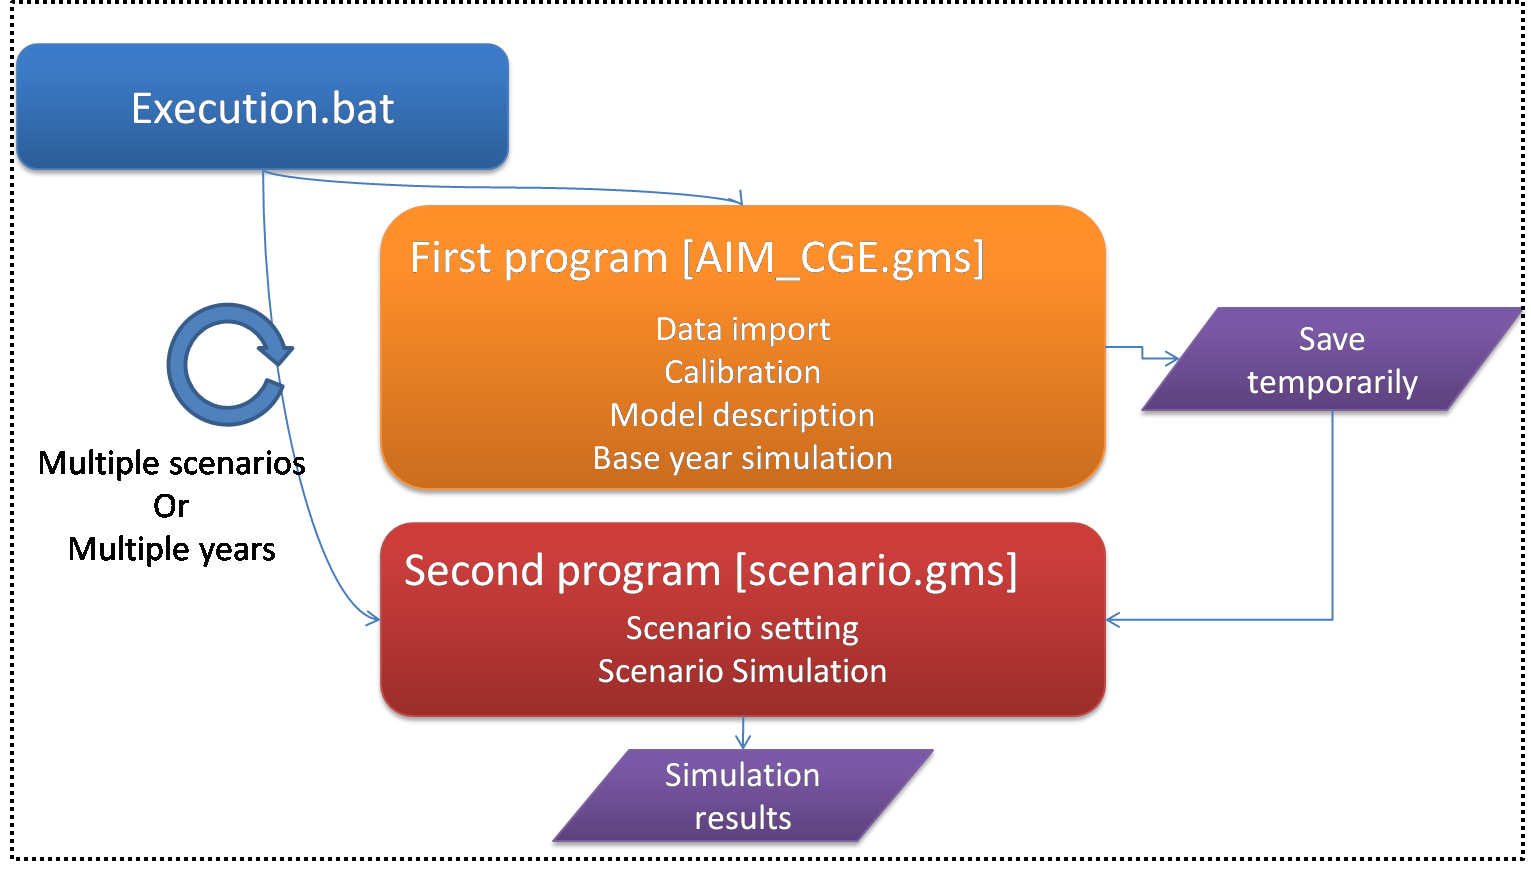
\includegraphics[width=1\textwidth]{fig/image10.png}
\caption{Overview of the program structure}
\label{fig:OverProg}
\end{figure}
   [AIMHub.gms] consists of mainly 7 parts (without declaration of sets, parameters, variables and so on). 

The structure of [AIMHub.gms] is drawn in \ref{fig:AIMCGEStruc}. Left-side boxes represent the 7 procedures and some program files are included in each procedure, so the program names are shown in right side of that figure. The list of the components and their contents are described \ref{fig:AIMCGEStruc}\footnote{This list includes the declaration of sets, parameters and so on. The number of the sections shown in second column corresponds to that of in the actual program.}.[scenario.gms] includes following assumptions shown in \ref{tab:List of key assumptions}.
\begin{figure}
\includegraphics[width=1\textwidth]{fig/picture1.png}
\caption{\label{fig:AIMCGEStruc}AIMHub.gms structure}
\end{figure}

\begin{table}
\caption{\label{AIMCGE.gmscomponents}List of AIMHub.gms components}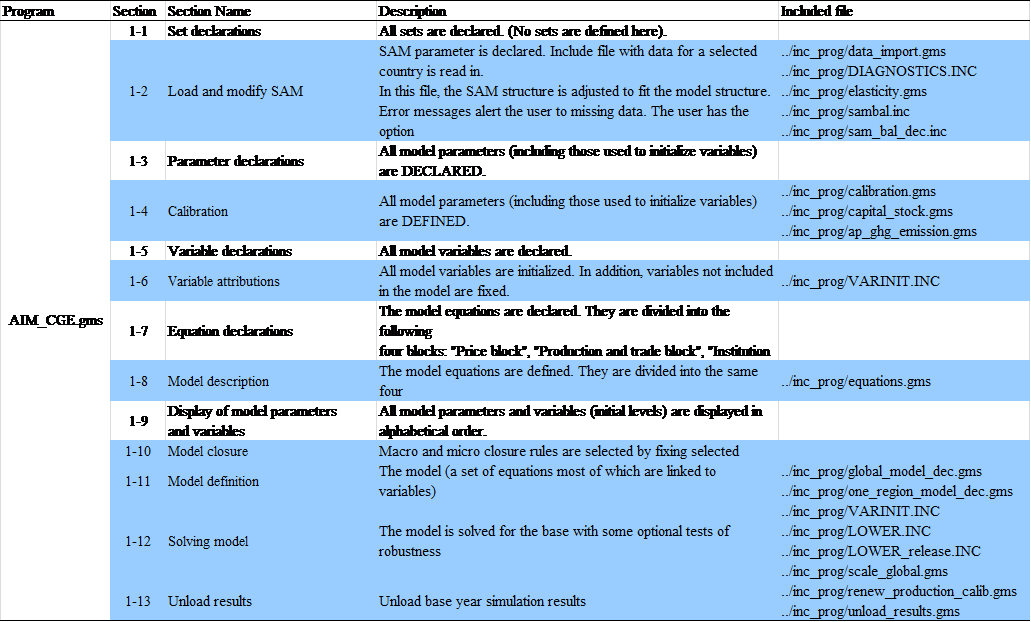
\includegraphics[width=1\textwidth]{fig/image12.png}
\end{table}
\section{\label{sec:HowtoRunModel}How to run the model}

There are two ways to run. One is using batch file and the other is shell. From Oct 2021, batch file operation is no longer updated and using shell is highly recommened. 

For shell users, the execution of the model is done by execute a shell file \seqsplit{/shell/execution\_global.sh}. This execution batch file includes setting file \seqsplit{shell/settings/execution01.sh} which specifies several model execution parameters. For users, please copy execution01.sh and execution\_global.sh into same directories respectively and use them so that they are kept as default settings of shell configuration. The execution parameters can be classified into two. One is about the process parameters and the other is model settings.

For batch users, these two corresponding files are batch/execution\_global.bat and batch/settings/execution01.bat.

Warning: During the running procedure, when multiple windows are open and one window request you to press any key to continue, be careful not to push it at the wrong time. When only one window is open, it is OK to push any key to continue.

\section{\label{sec:ProPar}Process parameters}

The execution process can be divided into eight as shown in Figure \ref{fig:ProcFlo}. It starts from base year balancing and parameter declaration (1). Then, calibration and base year simulation is made (2). After that, future year simulation is preceded (3). Latter processes are the translation of CGE model variables into analytical indicators. Merge gdx for all years is done for each scenario (4) and next is making analytical output for each scenario (5). These 4 and 5 proceudres keep annual information as they are computed. Then, all scenario results are combined (6) which limits the information to every 5 year step. This process (6) is no longer main stream of results synthesizing as of July 2021. Process (7) is done for making IAMC template which is required to submit any scenarios to IIASA database. This process (7) is run for each scenario keeping annual information. Also, MAGICC run is carried out within this process. Finally, IAMC template of all scenarios are merged into single GDX file in (8).
\begin{figure}
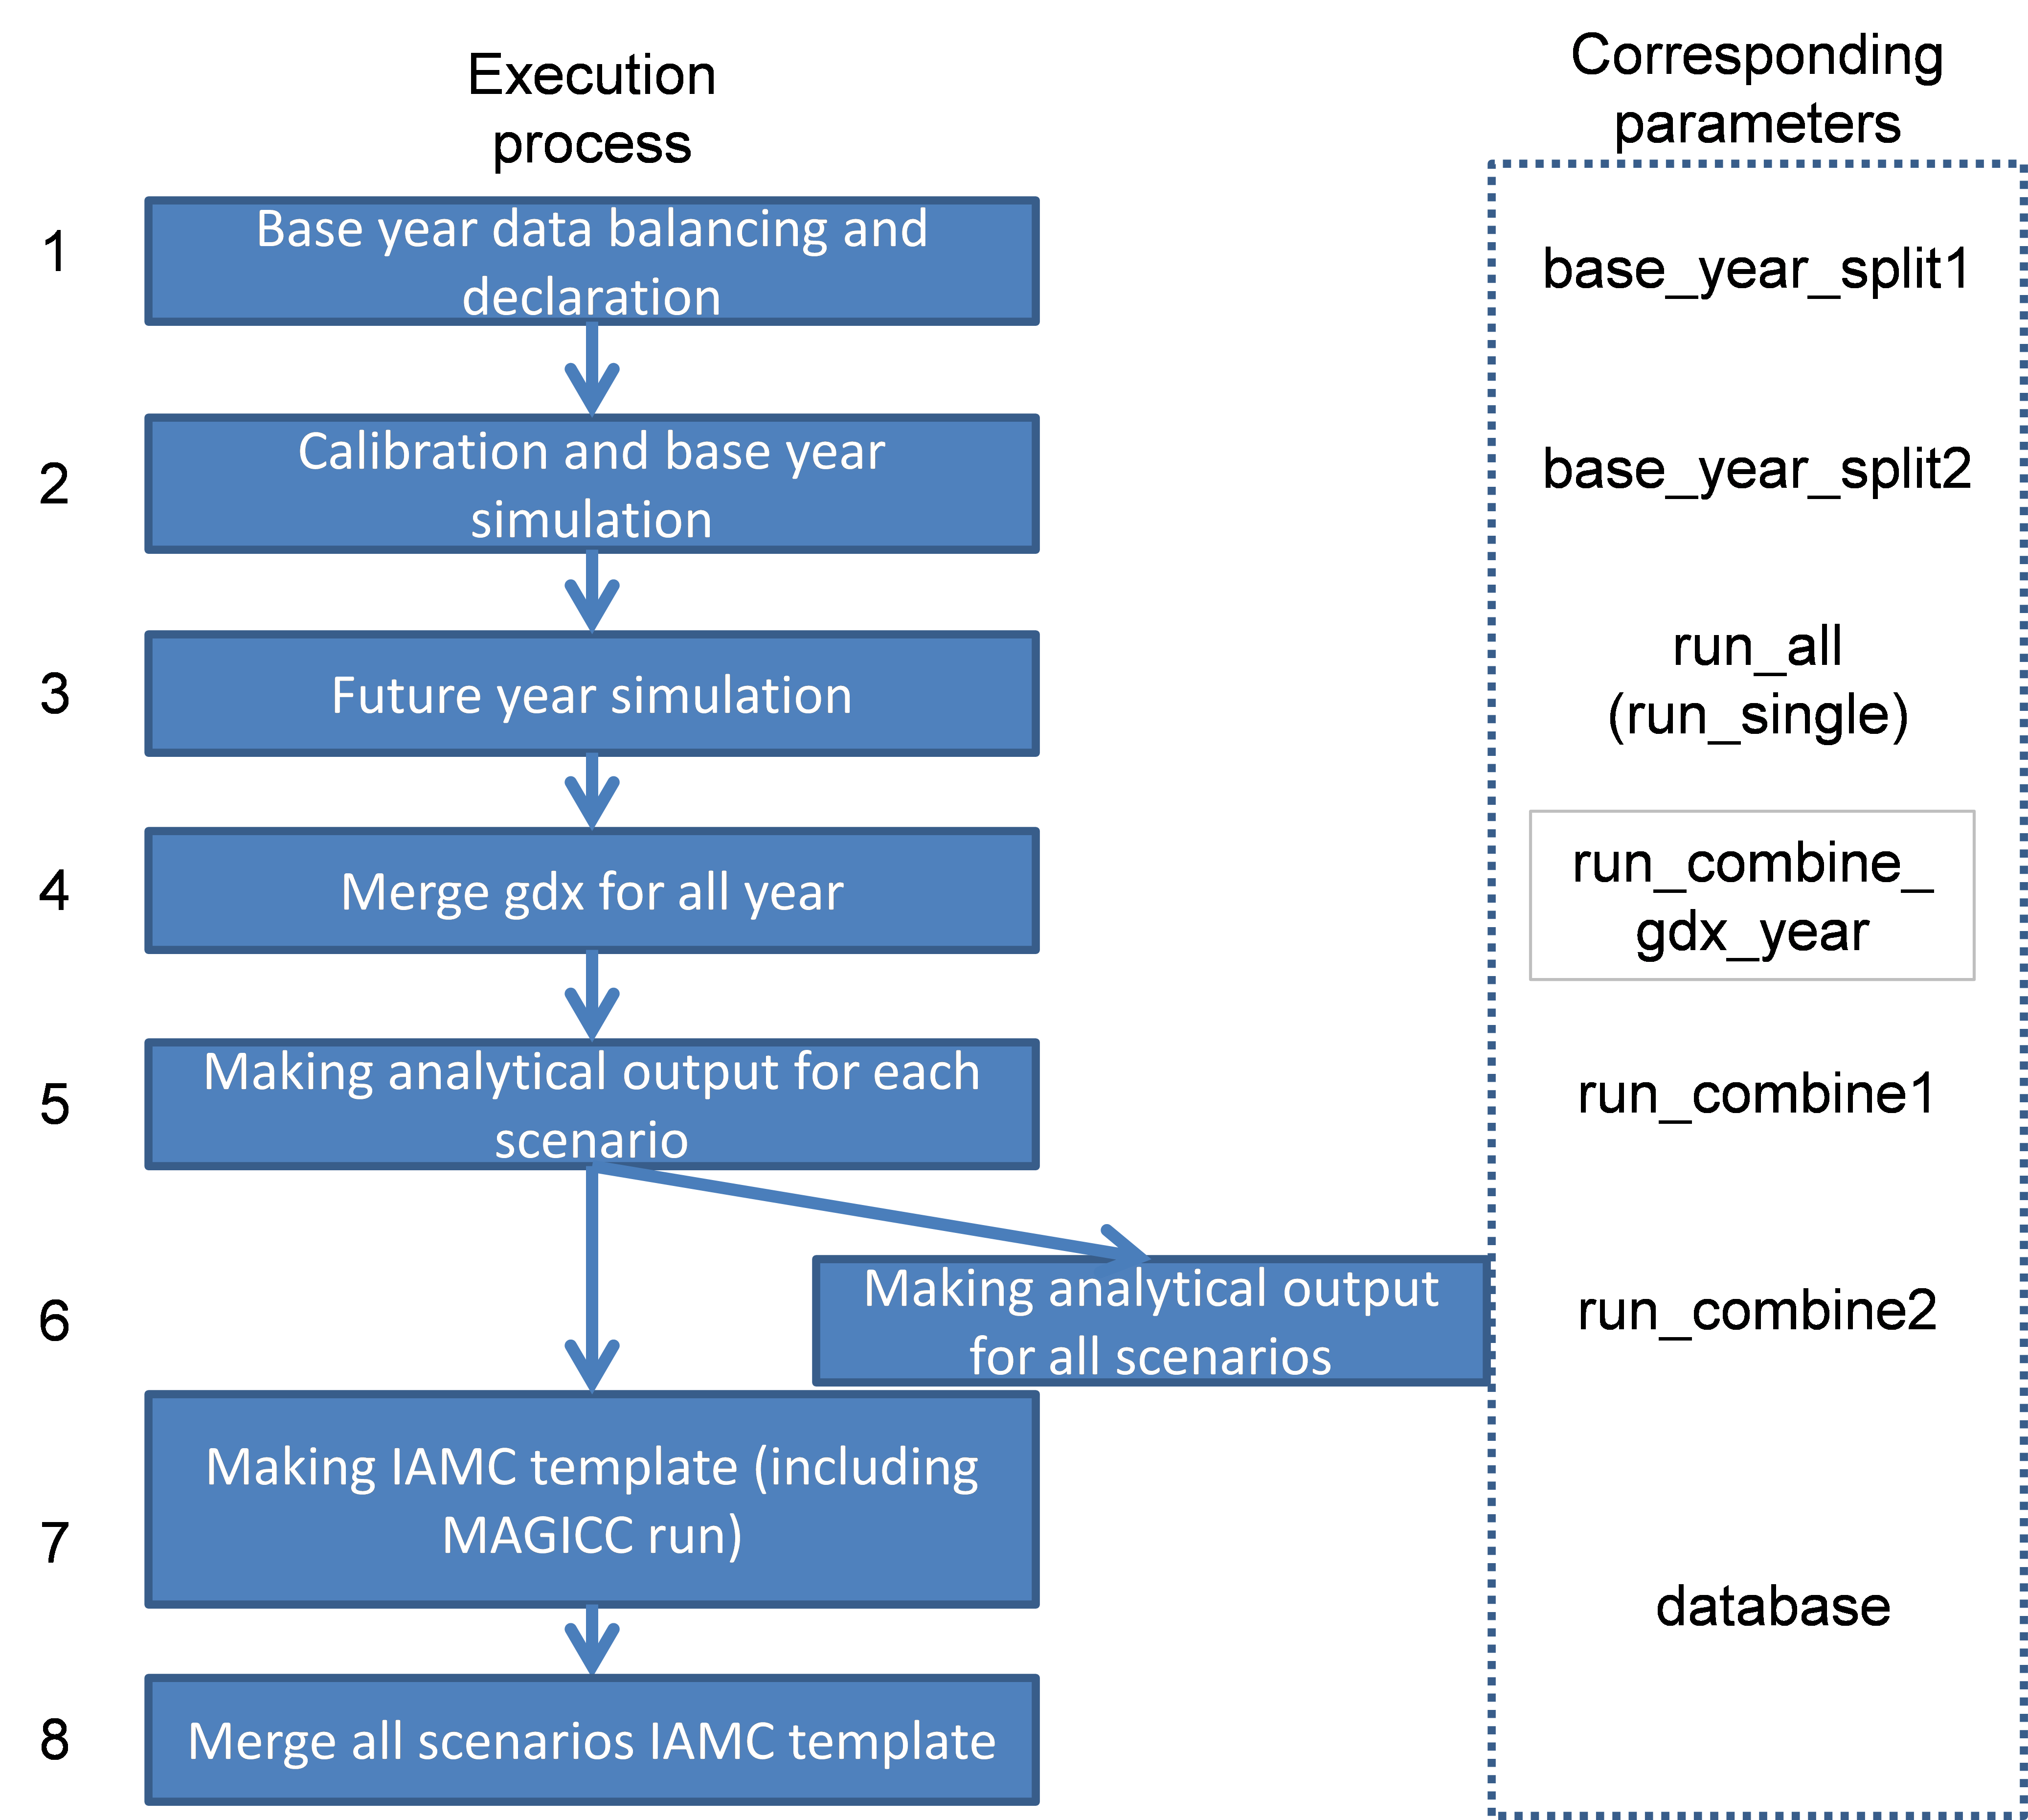
\includegraphics[width=1\textwidth]{fig/image13.png}
\caption{\label{ref-0070}Process flow of the AIM/CGE model execution and corresponding parameters}
\label{fig:ProcFlo}
\end{figure}
From version 2.3.2, the users can specify CPU threads numbers that the users would like to use. Then, the shell script automatically allocates the jobs to threads. There are other several remarks as below.

Some notes:
\begin{itemize}
\item XXX\_BaU\_NoCC should be run at the first time regardless of socioeconomic assumptions. After getting combine1 process for XXX\_BaU\_NoCC, you can run mitigation or impacts cases changing the ''BaU'' and ''NoCC'' terms. This is because under BaU\_NoCC scenario, some parameters such as TFP and household consumption preferences are calibrated.
\item If you run base\_year, usually you don't need to run anymore. Only when you have revisions of original data or basic structure of models, you need to rerun .
\item Run\_single is usually used for debugging the year where you find solution errors. This option allows you to run the year which you want to run and stop the simulation at that year.
\item Run\_combine\_gdx\_year is merging gdx process so that it cannot be paralleled even if you had many scenarios.
\item For mulple scenario parallel runs, you should turn off ''run\_all'' and ''run\_single''.
\end{itemize}

\begin{description}
\item[set rmScenarioDataAll=on] remove GDX output files.
\item[set base\_year\=off] base year run (loading and balancing SAM, base year calibration and base year run) (''on'' for the first operation when you first receive the model)
\item[set run\_all=on]future years' run (all years) (no longer used from October 2021)
\item[set run\_single=off]future year's run but each year the ''pause'' command is used
\item[set run\_combine1=on]making analytical gdx for one scenario
\item[set run\_combine2=on]combining all results across scenarios and make results files.
\item[set run\_all\_parallel=off]future years' run (all years) with multi-process parallel run
\item[set database=off]running climate model and making a csv file for IIASA database template model results (This function is outdated from July 2021)
\item[set NCPU=8]Specifying number of cores that are used for the pararell process
\item[set pausemode=off]If you would like to pause each process, turn on this switch
\item[set MultiSol=3]If you would like to use multi-threds, specify the number and 1,3, or 5 are currently available. Be careful number of NCPU, scenarios and this MultiSol. \$scenarios*\$MultiSol will be parallelly used. 
\item[set pridspe=3]If you would like to debug and see the difference of the MultiSol condition, specify the numbers. This option is linked to MultiSol. 
\item[set SceNameSpe=off]If you would like to specify IAMC template scenario names, turn on this switch and specify the scenario mapping ../tools/iiasa\_database/define/scenario.map. 
\item[set VisSceNameAuto=off]If you would like to automatically assign the scenario names for visualizatoin, it should be on. otherwise it should be off.

\end{description}
on/off are options for all parameters

\section{\label{sec:ModSetPar}Model setting parameters}

Table \ref{tab:modelsetting} shows list of model setting parameters. CLP and scenario\_name can have multiple codes (e.g. SSP2 and SSP3 for scenario\_name) and if you choose parallel process parameters on, the scenarios run in parallel. However, to run climate policy scenarios (not BaU) you have to finish BaU running process (for ''combine\_gdx\_year'' and ''combine\_gdx1'' in advance since climate policy cases use BaU results. In shell files, if you would like to multiple parameters for a particular set below, you should double quote with space seprates (e.g. CLP=''BaU CM'').

If you define new scenarios or climate policy cases, you have to change settings in tools as follows.


\begin{tabularx}{\textwidth}{|
p{\dimexpr 0.196\linewidth-2\tabcolsep-2\arrayrulewidth}|
p{\dimexpr 0.13\linewidth-2\tabcolsep-\arrayrulewidth}|
p{\dimexpr 0.136\linewidth-2\tabcolsep-\arrayrulewidth}|
p{\dimexpr 0.538\linewidth-2\tabcolsep-\arrayrulewidth}|} 
\caption{model setting parameters\label{tab:modelsetting}} \\
\hline 
parameters & Default value & Alternative options & Description \\\hline 
global & on & Off & Specification of global model or single country model \\\hline 
Sr & JPN & 106 regions & Code of country if the model is used as single country model. Regional codes are listed in the manual. \\\hline 
base\_year & 2005 & None & Base year \\\hline 
target\_year & 2050 & 2100 & Last year of target period \\\hline 
Start\_year & 2006 & Any from base to target year & The starting year of scenario run. Basically 2006 is preferable but for when the users check the model results and conditions in case the users encounter errors \\\hline 
CLP & BaU & CTAX, 26W, 37W, 45W, 60W etc. & Specification of climate policy. BaU does not have any constraint on emissions nor emission price while the others have. The strength of the constraint depends on the scenarios. The emissions cap or emission price is described in the prog /scenario/emission/***.gms \\\hline 
IAV\_ass & NoCC & CC1 etc. & For the IAV analysis, climate change condition can be specified by this switch. \\\hline 
Scenario\_name & SSP2 & SSP1-SSP5 and any & Scenario name that specifies socioeconomic assumptions. The name is freely available. Corresponding socioeconomic scenario should be specified in the prog/scenario/socioeconomic/***.gms  \\\hline 
Enduse & on & Off & If detailed Enduse technological information is used, then turn on. It increases computational burden almost double. \\\hline 
RunExclude & "" & Any scenarios & List of scenarios that are not run. \\\hline 
\end{tabularx}

\subsection{\label{subsec:SocAssLis}Socioeconomic assumptions list}

''scenario\_name'' specifies the socioeconomic assumptions. Currently a list of default scenarios is shown in the table in Table \ref{tab:SocAssList}.


\begin{tabularx}{\textwidth}{|
p{\dimexpr 0.203\linewidth-2\tabcolsep-2\arrayrulewidth}|
p{\dimexpr 0.797\linewidth-2\tabcolsep-\arrayrulewidth}|} 
\caption{\label{tab:SocAssList} Socioeconomic assumptions list} \\
\hline 
Scenario\_name & Description \\\hline 
SSP1-SSP5 & Shared Socioeconomic Pathways (SSPs) default five scenarios. Details are in Fujimori et al. (2017)~\cite{RN4363} \\\hline 
SSP2\_hindcast & For hindcasting simulation of which details are shown in Fujimori et al. (2016)~\cite{RN4011} \\\hline 
SSP2i & Basic assumptiosn are SSP2 but currently planed policies are reflected. Details are shonw in Roelfsema et al.~\cite{RN4407}. Currently (July, 2020), this would have very little impacts since IEA Energy balance is reflected until 2015.  \\\hline 
SSP2\_AIMEInv & AIM/Enduse energy system information is reflected which is only avaialbe for Japan (July, 2020). Details are shown in Fujimori et al. (2019)~\cite{RN4425}. \\\hline 
SSP2\_CGEG & CGE global results are again fed into the simulation so that carbon tax effects to change price conditions are isolated. \\\hline 
\end{tabularx}
\subsection{\label{subsec:CliPolAssLis}Climate policy assumption list}

''CLP'' specifies the climate policy assumptions. Currently a list of default assumtpions is shown in table \ref{tab:CliPolAssList}. 
For the global constraint scenarios, CarBud should be also specified as carbon budget from 2020 to 2100.


\begin{tabularx}{\textwidth}{|
p{\dimexpr 0.22\linewidth-2\tabcolsep-2\arrayrulewidth}|
p{\dimexpr 0.17\linewidth-2\tabcolsep-\arrayrulewidth}|
p{\dimexpr 0.65\linewidth-2\tabcolsep-\arrayrulewidth}|} 
\caption{\label{tab:CliPolAssList}Climate policy assumptions list} \\
\hline 
Scenario\_name & Global/ National & Description \\\hline 
BaU & Global/ National & Without any climate policy. This scenario should be run firstly to calibrate TFP. \\\hline 
EmiTar2030\_CONT1 & Global & 2030 emissions target is met and then continue equivalent effort. \\\hline 
EmiTar2030EtOn & Global &2030 emissions target is met with the emissions trading and then continue equivalent effort. \\\hline 
EmiTar2030\_CONT3 & Global &2030 emissions target is met and then continue equivalent effort using carbon tax. \\\hline 
2020NDC\_NZE & Global &for 2030 updated NDC is met and then goes net zero in 2050 based on current announcement. \\\hline  
2020NDC\_NZE2030EtOn & Global &for 2030 updated NDC is met and then goes net zero in 2050 for all countries with emissions trading. \\\hline
2020NDC\_NZECO & Global &for 2030 updated NDC is met and then using global constraint goes net zero in 2050. \\\hline 
2020NDC\_NZEAll & Global &for 2030 updated NDC is met and then goes net zero in 2050 for all countries with emissions trading. \\\hline 
CO2F1\_CACN & Global &global emissions constraint from 2020. \\\hline  
CO2F1\_2025CP & Global &global emissions constraint from 2025. \\\hline 
CO2F1\_2015INDC & Global &global emissions constraint from 2030 after INDC emissions constraint made in 2015. \\\hline 
CO2F1\_2020NDC & Global &global emissions constraint from 2030 after updated NDC emissions constraint made in 2020. \\\hline 
20W, 26W, 34W, 45W, 60W & Global & Stabilizing radiative forcing at 2100 roughly corresponding values. The global uniform carbon price for all sectors and GHGs start from 2015. \\\hline 
CTAX100, CTAX1000 & Global/ National & Carbon price path starting from 2021 and linearly connect to 2100 by 100 or 1000\$/tCO2.  \\\hline 
\end{tabularx}

\begin{table}
\caption{\label{ref-0078} Country code list}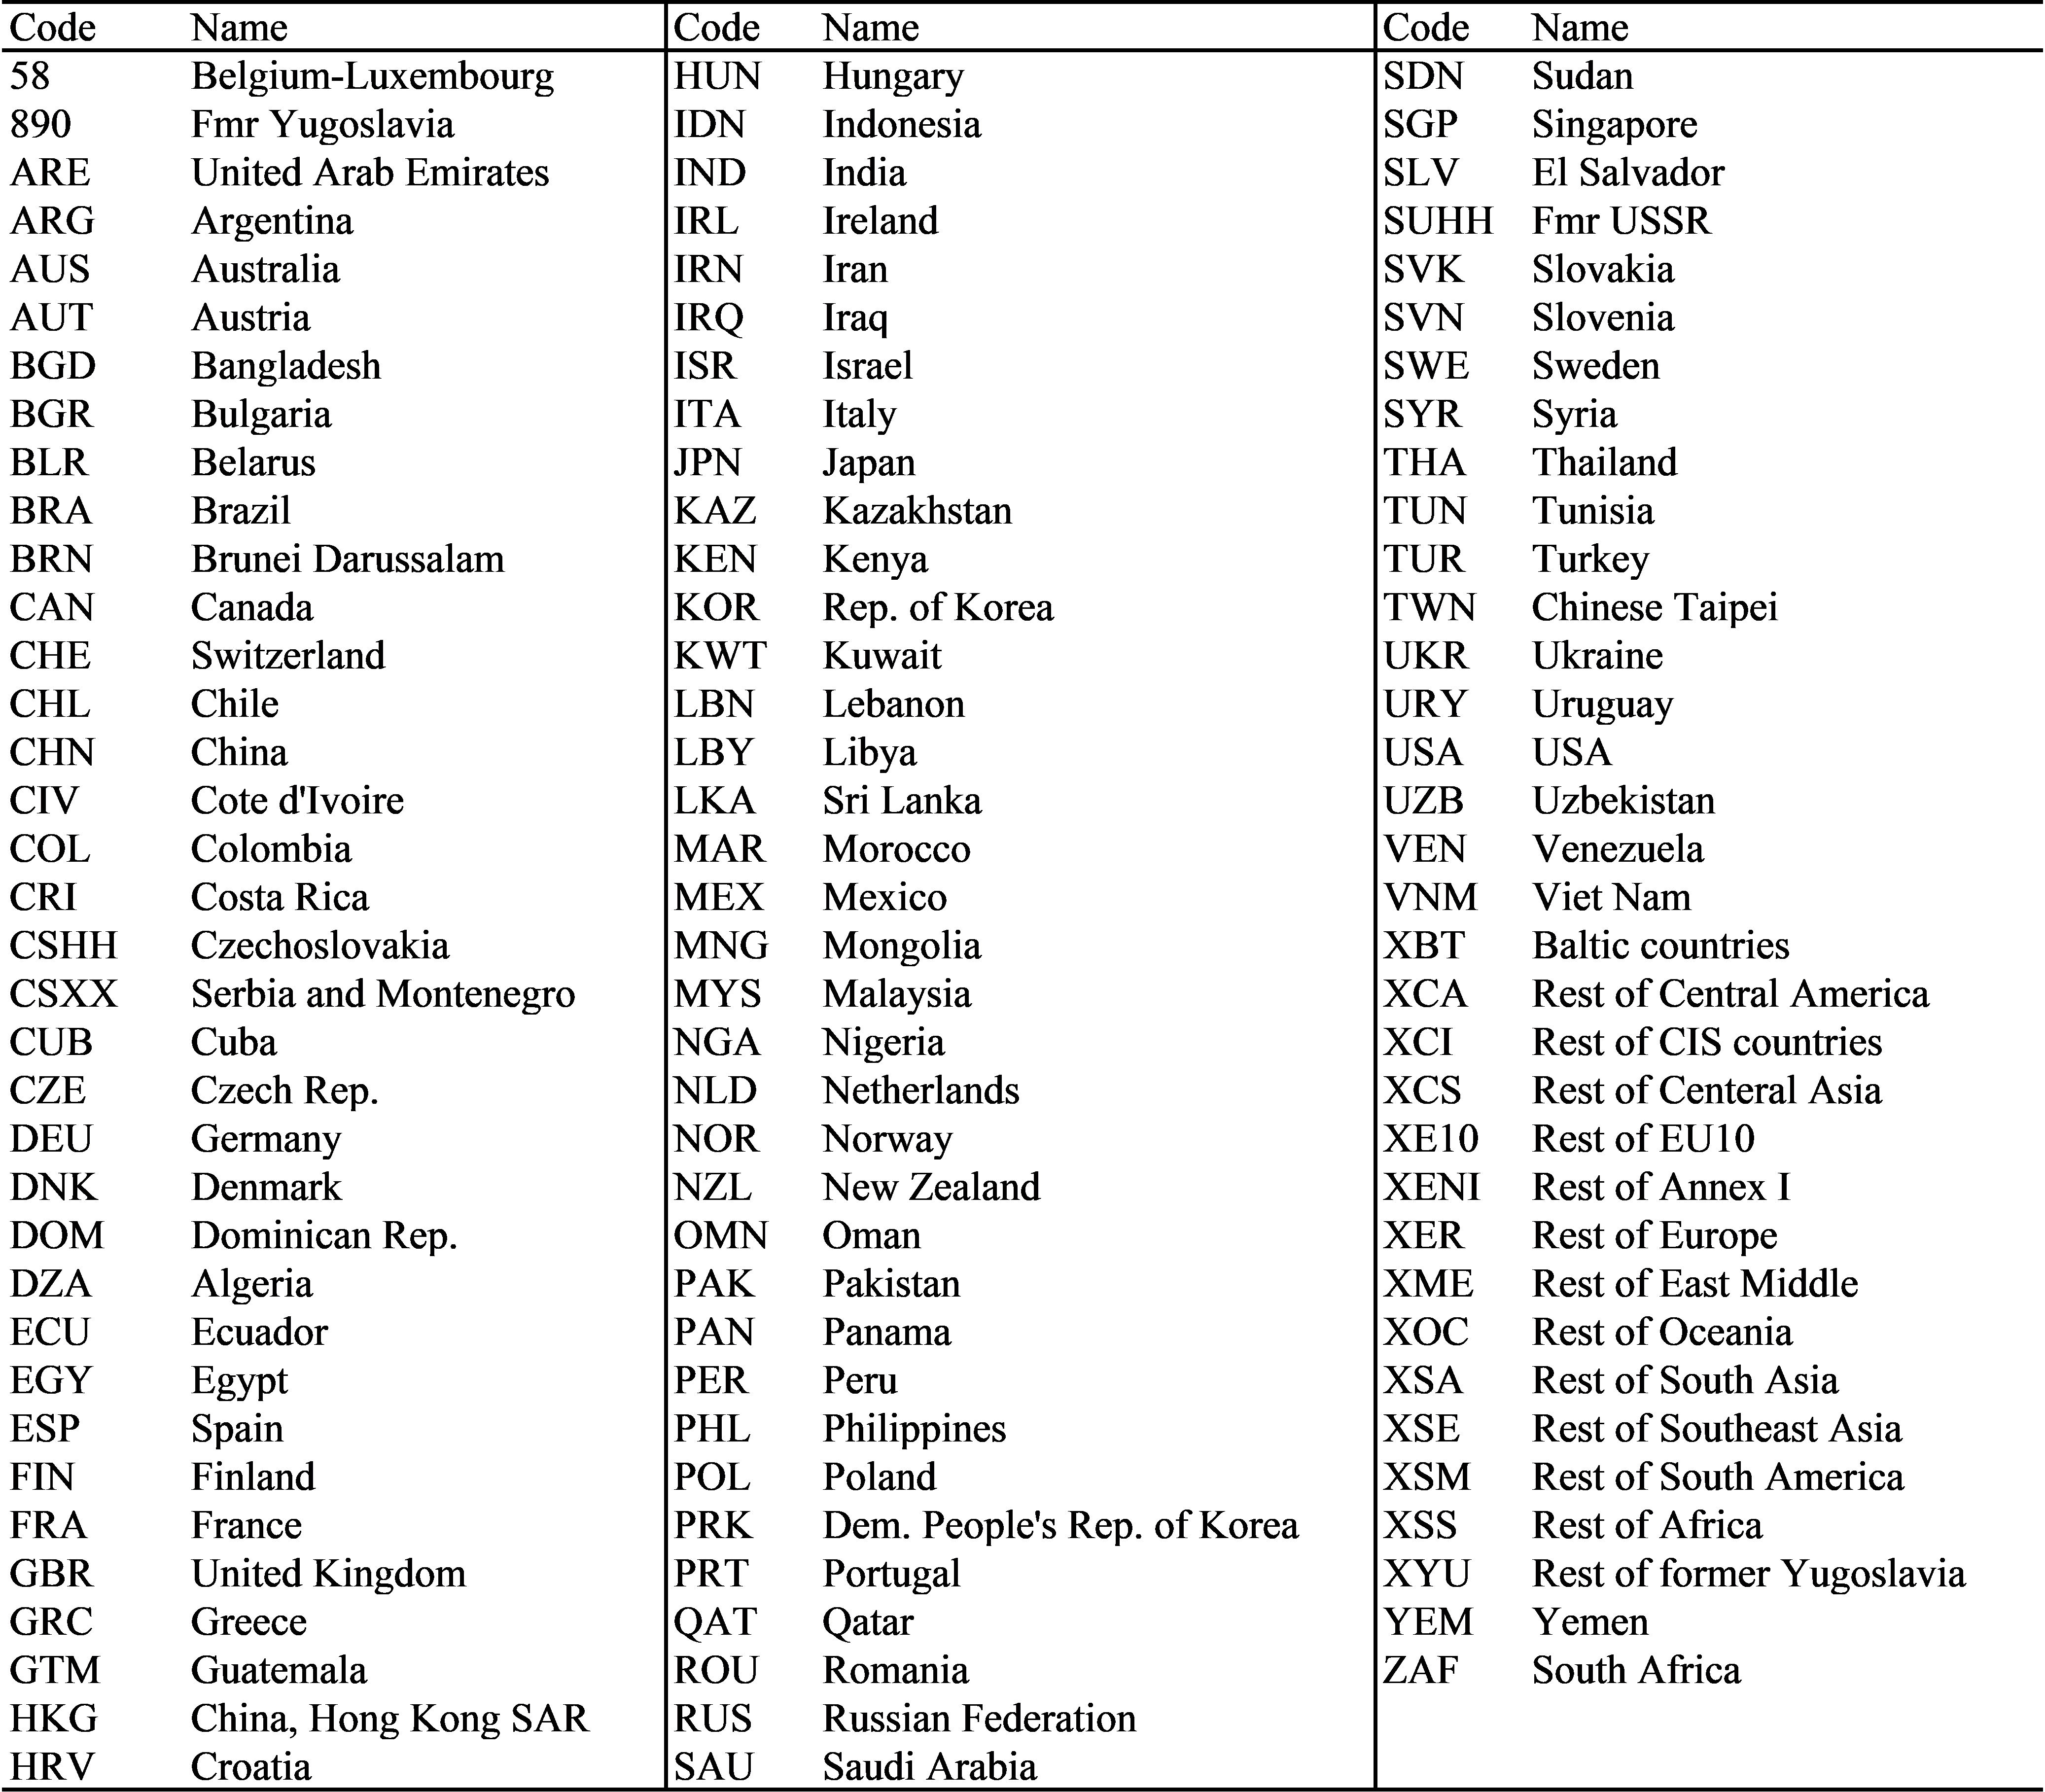
\includegraphics[width=1\textwidth]{fig/image14.png}
\end{table}
 

\begin{landscape}
\begin{tabularx}{\textwidth}{|
p{\dimexpr 0.15\linewidth-2\tabcolsep-2\arrayrulewidth}|
p{\dimexpr 0.23\linewidth-2\tabcolsep-\arrayrulewidth}|
p{\dimexpr 0.19\linewidth-2\tabcolsep-\arrayrulewidth}|
p{\dimexpr 0.45\linewidth-2\tabcolsep-\arrayrulewidth}|} 
\caption{\label{tab:List of key assumptions} List of key assumptions in scenario.gms }
 \\
 \hline
Flag & file name & Assumption name & Contents \\ 
 \hline\hline
 \endfirsthead
 \multicolumn{4}{l}{\small\it conrtinued from previous page}\\
 \hline
Flag & file name & Assumption name & Contents \\ 
 \hline\hline
 \endhead
 \hline
 \multicolumn{4}{l}{\small\it contibue to the next page}\\
 \endfoot
 \hline
 \multicolumn{4}{l}{\small\it finish}\\
 \endlastfoot

Assumption001 & scenario.gms \newline inc\_prog/030\_close\_act2.gms \newline inc\_prog/030\_parameter\_in.gms \newline inc\_prog/030\_close\_act.gms & Closing small sectors Closing sectors that have small activity levels & Closing sectors that have small activity levels. This treatment is needed to avoid infeasible solution due to the small numbers \\\hline 
Assumption002 & scenario.gms & Specifying emissions gases that are exempted from emissions tax & Some sectors could cause infeasibility due to very high emissions penalty associated with emissions tax and to avoid this situation, some non-energy related emissions are exempted. The default sectors are as below.
\begin{itemize}
\item Coal mining, oil extraction and gas extraction
\item Forestry
\end{itemize}
 \\\hline 
Assumption003 & scenario.gms & Power generation cost calibration & The base year power cost information may have some issues and make 2006-2010 as calibration period. The basic idea is to assume following standard technological information. \newline 
\begin{itemize}
\item Investment cost
\item Life time
\item Operation and Management cost
\item Capacity factor
\item Cost share of transmission and distribution
\end{itemize}
The actual assumptions are in /data/TechnoEconomic.gdx. \newline From 2006 to 2009, the production function input coefficients are adjusted to match with the data shown in Table \ref{tab:CapFac} to Table \ref{tab:CostShareTra}. The cost decreases and capacity factor changes for the further period are assumed as shown in the tables. \newline This treatment without forcing the energy consumption to IEA Energy Balance Table, the power price changes happen, which actually show something strange behavior in electricity consumption. Thus, IEA Energy Balance calibration option for this period should also be implemented simultaneously. \\\hline 
Assumption004 & scenario.gms & Power generation and biomass nesting share parameter shift & \color{red}{The logit share parameter (psiac) is controlled by this assumption but it should be noted that here the assumptions are quite strong}. \newline Power sector; \newline The logit share parameter (psiac) is basically calibrated IEA Energy balance table until 2015. For BaU scenario, they are kept as they are afterwards. For mitigation scenario, after carbon price occurs, the bias currently existing in the renewable energy is diminished and it is assumed that the share parameter has equal value in fossil and renewable (win, spv and bio) in 2050 (sum of renewable = sum of fossil).  \newline Biomass; \newline For second generation (residue and energy crops) bioenergy, the shift parameter is to be equal in 10 years. The first generation bioenergy is to decrease by 1 \%. \\\hline 
Assumption005 & scenario.gms \newline inc\_prog/030\_PopGDPScenario.gms & GDP and population assumptions & GDP and population are assumed as indicated in the socioeconomic assumption files. \\\hline 
Assumption005-1 & scenario.gms & Hindcast capital formation and price assumptions & Capital formation and price assumptions for hindcasting mode \\\hline 
Assumption006 & scenario.gms \newline inc\_prog/030\_aeei\_adjustment.gms & AEEI assumptions & AEEI assumptions that are described in Fujimori et al.~\cite{RN4363}. For the total energy consumption, the AEEI is associated with GDP growth. For the energy carrier-wise AEEI, basically shift from the dirty (coal) to cleaner (electricity) is assumed.  \\\hline 
Assumption007 & scenario.gms & Energy service demand parameter  & For default mode, transport service is the main parameters to be changed. However, current model does not determine the energy consumption in transport sector is determined by the CES function and disaggregation of the mode specific energy consumptions are derived from the base energy service which can be controlled by this parameter assumption. \\\hline 
Assumption009 & scenario.gms & Change saving ratio & The saving ratio assumptions but it is usually unused because the investment is exogenous and saving rates are endogenous variables. \\\hline 
Assumption010 & scenario.gms \newline inc\_prog/020\_biopotential.gms & Biomass fuel potential for wood and agricultural residue & \color{red}{Agricultural residue are computed by previous year's crop production with coefficient which is computed by base year FAO information. Wood residue is also associated with forestry sector's activity level. 50\% of both technical potential can be used for the energy purpose.} \\\hline 
Assumption011 & scenario.gms & Nonenergy use rate (this is only for the detailed Enduse technology representation mode) & Non energy use assumptions but it is only for the Enduse technology on mode which is rarely used now (July, 2020) \\\hline 
Assumption012-1 & scenario.gms & Plantation rotation assumption & \color{red}{The assumptions related to plantation rotation. Basically base year Co2 sequestration. This is closely related to the description at ''*Wood removal for wood production'' in ap\_ghg\_emission.gms} \newline \color{red}{The base year assumption is that 90\% of wood removal (industrial and fuel wood) in high countries are well managed so that the trees are planted after wood is removed. 50\% and 10\% are assumed for middle- and low-income countries. The income classifications are made by 12616, and 3323\$/cap, respectively.} \newline \color{red}{For the future, in 2050 all countries' planation situation catch up with the high income countries' assumptions.} \\\hline 
Assumption012-3 & scenario.gms & VRE Curtailment and storage & Assumptions related to VRE curtailment and storage. The parameters are shown in Dai et al.~\cite{RN4366}. Basically storage is needed if the share of solar exceeds 5\%.  \\\hline 
Assumption012-5 & scenario.gms \newline inc\_prog/030\_EneModelload.gms & Energy model loading assumption &  The energy system model (energy statistics information) is incorporated. The method is fully described in Fujimori et al.(2019)~\cite{RN4425}. For the IEA Energy balance table implementation, from 2007 to 2019 are used. 2006 is the special year which has new stock and many model parameters can change and thus to avoid too much jump in 2006, the IEA Energy Balance starts from 2007. Currently, the CCS rates are not fully taken into account (July, 2020). \\\hline 
Assumption013 & scenario.gms \newline /inc\_prog/030\_basescenario.gms & TFP and other related assumptions & Labor force and capital stock assignment to parameters and TFC assumptions.  \\\hline 
Assumption013-1 & scenario.gms \newline ../inc\_prog/ \newline ResourceAssumptionVRE.gms & Variable renewable energy supply cost and capacity & VRE renewable energy potential and cost curve is assumed. Basically, there are 5 grades to cut the supply curves and we compare the previous year's production level with these curves and determine the production cost. The curve information is from Silva et al. (2016)~\cite{RN4380}. \\\hline 
Assumption013-2 & scenario.gms  \newline /inc\_prog/030\_renewable\_prodcutoin.gms & Install renewable energy (not existing in the previous year) & Renewable energy, nuclear, storage industry installation that do not exist in the previous year's calculation.  \\\hline 
Assumption013-3 & scenario.gms  \newline /inc\_prog/030\_CCS\_industry.gms & Install CCS plant & Installation of CCS technology industry \\\hline 
Assumption013-4 & scenario.gms  \newline /inc\_prog/030\_BaU.gms  \newline /inc\_prog/030\_NonBaU.gms & BaU or NonBaU specific assumptions & BaU or non BaU scenario specific assunmptions (see assumptions inside of the file as below assumptions 1XX) \\\hline 
Assumption013-5 & /scenario/BaU.gms & Renewable energy capacity constraints in BaU scenario & \color{red}{Bioenergy, geothermal, other renewable have 2\% growth limit. For nuclear, if the country has more than5\% of nuclear in power generation, the maximum increase rate is GDP growth rates. Otherwise, 20\% is the maximum increase rate.} \\\hline 
Assumption013-6 & scenario.gms \newline inc\_prog/030\_EneModelload2.gms & Energy model loading assumption second & This second specification is mainly for the scenarios having carbon price and thus this part is located later than the inclusion of NonBauU.gms. \\\hline 
Assumption014 & scenario.gms & Power generation constraints (If the quota is finished but there are some years) & If power generation constraint is applied in earlier years, the computed complementary variable for that constraint which is interpreted as part of share parameter of logit function is applied to the later period. \newline Parameters ''Prenew\_up'' and ''power\_share\_up'' are cancelled if quota is assumed. \\\hline 
Assumption015 & scenario.gms & Energy substitution & Energy substitution for the transport electricity and biofuel are adjusted. \\\hline 
Assumption016 & scenario.gms & Transport energy efficiency & Transport mode-wise energy efficiency parameter changes. The total energy consumption is determined by the CES aggregates and this can be effective only look at disaggregated transport mode-wise energy consumption. \\\hline 
Assumption017-1 & scenario.gms & Biopotential supply curve & The biomass energy crop potential supply curve information is loaded. The original data is AIM/PLUM model output~\cite{RN3982}~\cite{RN4448}. The original gridded data is classified into 8 grades for each region and the bioenergy supply volume in the previous year is compared with that supply curve. \\\hline 
Assumption017-2 & scenario.gms \newline inc\_prog/030\_biofuel.gms & Bioenergy industry assumptions & Bioenergy industry assumptions. Details are described in Fujimori et al. ~\cite{RN4520}\\\hline 
Assumption017-4 & scenario.gms & F-gas emissions & F-gas emissions reduction assumptions which is described in SSP paper ~\cite{RN4363}. The original assumption comes from IMAGE team. \\\hline 
Assumption017-3 & scenario.gms \newline inc\_prog/030\_air\_pollutant\_scenario.gms & Air pollutant scenario & Assumptions on the air pollutant emissions which is described in SSP papers~\cite{RN4363}~\cite{RN4360}. The original data comes from GAINS team.  \newline There are some critical own assumptions to the baseline. \newline 
\begin{itemize}
\item For agricultural emissions, 0.125, 0.25 and 0.5\% annual decrease rates in the emission factors are applied for weak , central and strong air pollution policies respectively.
\item For forest related emissions, 0.25, 0. 5 and 1.0\% annual decrease rates in the emission factors are applied for weak , central and strong air pollution policies respectively.
\item For waste related emissions, 0.25, 0. 5 and 1.0\% annual decrease rates in the emission factors are applied for weak , central and strong air pollution policies respectively.
\item For the energy-related emissions but missing in GAINS in some species, we assume 2\% per annual improvement in the emission factors.
\end{itemize}
For the biofuel which does not exist in base year, we adopt petro emissions factors. \\\hline 
Assumption018 & scenario.gms & Fossil fuel extraction & Coal, oil and natural gas extraction cost assumptions. The original data is from Rogner et al.~\cite{RN2677} which has 5 grades. The volume of cumulative extraction is considered to mark-up the production cost. 5 grades are linearly interpolated to avoid the sudden cost increase at some point. \\\hline 
Assumption018-5 & scenario.gms & Electricity distribution loss improvement & The electricity distribution loss rate is assume to have 1\% annual improvement (for example, if the distribution loss is 10\% in the base year, next year will be 9.9\%=0.1*0.99), but the minimum value is set to 4.5\% which is current Japan's rates. \\\hline 
Assumption019 & scenario.gms & Agriculture yield scenario & For crops, there are two types of yield assumptions; namely default and shock cases. The former is the default technological change assumptions described in Hasegawa et al.~\cite{RN3987} which has SSP variations. The latter is mainly for the climate change yield shock and incorporates the crop model yield shock data. \newline \color{red}{For pasture land productivity, we assume that the productivity is improved by the expected livestock demand changes which are computed by GDP growth with income elasticity and population changes.} \\\hline 
Assumption020 & scenario.gms & Land use change long term shifter & \color{red}{For the land allocation logit function, the share parameter of the energy crop is assumed to shift to the average value of individual crop.} \\\hline 
Assumption021 & scenario.gms & Intermediate input coefficient change & Steel intermediate inputs coefficients changes based on Fujimori et al 2011~\cite{RN3451}. \newline These improvement rates come from Japan's numerical evidence from Committee on iron and steel statistics(Committee on iron and steel statistics, 2006)~\cite{RN4029} and STAN Database \textsuperscript{25}~\cite{RN2838}. The Committee on iron and steel statistics [4] contain steel order volume for each sector and the STAN Database (OECD [13]) has industrial output indexes. The steel consumption per unit production was then plotted as in the Figure 3.5 (Fujimori et al. 2011~\cite{RN3451}). Each industry experienced improvement in steel consumption intensity over the past three decades. This decrease is probably due to the substitution of steel with other materials such as plastics. However, we could not confirm that substitution with the evidence so far. Thus, we assume that the decrease in steel use would be homogenously replaced by the other material inputs. Based on the assessment, we assume 4.7\% (average of machinery and transport equipment) and 2.1\% for other manufacturing and construction sectors' input respectively. For the other heavy material goods, we don't so far solid evidence how the intermediate inputs changes over time and tentatively 2\% per annual are assumed. Those change rates, however, not directly applied to all countries uniformly because the countries which have relatively modest economic growth such as current high-income countries would have such rapid intensity of material use increase and thus, 80, 60 and 50\% of these improvement rates are adopted for the countries which GDP growth rates are 1-3, 0-1 and less than 0\% respectively. \\\hline 
Assumption021-1 & scenario.gms & Long-term trade share changes & There are three main assumptions on long-term trade function shift. \newline -~For biofuel and raw biomass, the trade and domestic share for both of import and export are eventually equal (determined by price) and thus 30 years later after trade occurs, the parameter shifted. \\\hline 
Assumption021-2 & scenario.gms & Trade tariff and export tax assumption change & Trade tariff and export tax rates changes. These are coming from socioeconomic assumptions. \\\hline 
Assumption022 & scenario.gms \newline inc\_prog/030\_CGEBoundary \newline Assumption.gms & CGE boundary conditions & Specification of total primary factor inputs, foreign direct investment, CPI, exchange rates, governmental consumption, governmental saving. Some of them are initial value and rest are fixed values for the model. \\\hline 
Assumption023 & scenario.gms & World trade price for national model & World trade price for national model, if there are global scenario named \%SCENAME\%\_\%Global4National\%, the corresponding world price is used for national model. \\\hline 
Assumption024 & scenario.gms & Transfer & Income (property and labor compensation) transfer assumptions of which increases are in line with GDP growth. \\\hline 
Assumption024-3 & scenario.gms \newline /inc\_prog/020\_foodwaste.gms & Food waste assumption & The food waste assumption is made. As stated in the socioeconomic\_assumptiong.gms there are two options whether the scenario considers SDG target to halve the food waste generated from consumption process.  \\\hline 
Assumption025 & scenario.gms \newline /inc\_prog/030\_hydrogen.gms & Hydrogen implementation & Hydrogen implementation. The way how hydrogen related industries are occurred is similar to bioenergy related industries. \\\hline 
Assumption026 & scenario.gms & GHG emission price initial value & Initial value for the GHG emissions price. This setting is critical to get solution in the year which firstly implement carbon price. The initial value should be sufficiently small to smoothly find solution. \\\hline 
Assumption027 & scenario.gms & Stock change decreasing & The stock change was assigned to some goods treated as physical volume in the model due to the inconsistency in the base year information. The calibrated stock change is assumed to decrease over the time period. \\\hline 
Assumption028 & scenario.gms & Non-energy related emissions abatement assumptions & Non-energy related emissions abatement assumptions. The exponential function is used. A similar method is already discussed by Hyman et al. (2003). The parameter is taken from Lucas et al. (2007)~\cite{RN2282} \\\hline 
Assumption029 & scenario.gms & International emission trading initial value and quota & 10-folds of BaU emissions are assumed to be the maximum export and import volume of emissions trading for global model. For national models, R\_EM\_TR(R) determines the ratios to the total emissions. Either way, CAP\_TRADE needs to be turned on. \\\hline 
Assumption029-1 & scenario.gms & International emission trading for kyoto protocol period & Emissions trading historical record (price and volume) for the Kyoto Protocol period taken from the World Bank report~\cite{RN3647}. \\\hline 
Assumption030 & scenario.gms & Landuse related emissions and their cost & \color{red}{There are two major assumptions related to land-use change emissions.} \newline \color{red}{First, if the afforestation option is off, the forest increases in mitigation scenarios should be lower than those in baseline.} \newline \color{red}{Second, we assume lower boundary for forest area if carbon tax is sufficiently high ({\textgreater}50\$) to avoid large deforestation. The actual assumption is that the previous year's forest area is lower boundary.} \\\hline 
Assumption031 & scenario.gms & Constraint for GHG cost of activity level (this is mainly for BioCCS) & BECCS related production activities (such as biomass power generation (E\_BIN) and biofuel refinery (BTR3) can get too much subsidy (negative carbon tax) under high carbon price, which makes negative production cost. This situation causes trouble in CGE solution and thus here the ceiling of the BECCS subsidy is assumed. The default (SSP2) maximum subsidy level is \color{red}{66\%} of production cost but varied among socioeconomic assumptions differentiated by BIOCCP.  \\\hline 
Assumption032 & scenario.gms \newline /inc\_prog/030\_biohygtrade.gms & Bioenergy and hydrogen trade assumption on/off & Bioenergy (liquids: COM\_BIO, primary energy crop: COM\_ECR) and hydrogen trade are assumed. /inc\_prog/030\_biohygtrade.gms is parameter specification for the initial year to implement these trades. The initial shares of import to the domestic consumption and export to the domestic supply are assumed to be 0.1\%. \\\hline 
Assumption033 & scenario.gms & Water consumption assumptions & Water consumption and withdrawal intensity coefficients are changed overtime. The improvement rates are differentiated by SSP assumptions where basically SSP1 and SSP5 have larger technological progress than SSP3 and SSP4, which leads double and half of the intensity improvement compared to SSP2. \newline Irrigation efficiency is improved by 0.2\% as default. \newline All assumptions are described in Fujimori et al. (2017, 2020~\cite{RN4200}~\cite{RN3985}) in detail.  \\\hline 
Assumption034 & scenario.gms & Consumption tax changes & For the cases which national models would like to change the consumption tax rate, it can be used. \\\hline 
  &   &   &   \\\hline 
Assumption102 & /scenario/BaU.gms & Power supply constraints from other literature (currently unused) & This part can implement exogenous power supply constraint for the individual technology but currently unused. \\\hline 
Assumption103 & /scenario/BaU.gms & Household preference parameter changes & LES parameters are changed based on income elasticity and income. This is mainly for the food consumption. \\\hline 
  &   &   &   \\\hline 
Assumption111 & /scenario/NonBaU.gms & GHG emissions constraints & Emissions constraint or carbon price path is adopted. \\\hline 
Assumption112 & /scenario/NonBaU.gms & Power supply constraints from other literature (currently unused) & This part can implement exogenous power supply constraint for the individual technology but currently unused. \\\hline 
Assumption113 & /scenario/NonBaU.gms & BaU's Productivity & BaU's TFP values is adopted. \\\hline 
Assumption114 & /scenario/NonBaU.gms & Trade elasticity changes & Change trade elasticity dynamically in non-BaU cases. \\\hline 
  &   &   &   \\\hline 
Assumption121 & /inc\_prog/030\_basescenario.gms & Labor force & Assignment of labor supply to the factor input parameter. \\\hline 
Assumption122 & /inc\_prog/030\_basescenario.gms & Capital stock & Total capital stock \\\hline 
Assumption125 & /inc\_prog/030\_basescenario.gms & TFP growth assumption & TFP assumptions for the scenarios that don't fix GDP in BaU (currently unused in July 2020) \\\hline 
Assumption131 & /inc\_prog/030\_aeei\_adjustment.gms & Fuel-wise energy efficiency improvement & Fuel-wise energy efficiency improvements are described. The traditional biomass, modern energy, coal use in building are differentiated.  \\\hline 
Assumption132 & /inc\_prog/030\_aeei\_adjustment.gms & Total energy consumption efficiency improvement & Total energy consumption efficiency improvement assumptions. The improvement rates are dependent on the GDP growth which reflect the development phases. Detailed assumptions are described in Fujimori et al.~\cite{RN4363} \\\hline 

\end{tabularx}

\end{landscape}

\section{\label{sec:SpecYearAssum}Specific years assumed in the model}

The model assumes some years that change the conditions such as new biofuel and hydrogen industries appear and so on.
Here is a list of such year (Table \ref{tab:LisSpecYear}) and these are specified in "/inc\_prog/030\_SpecYear.gms".
Note that these assumptions are overwritten if they are specidied in socioeconomic, climate policy or IAV assumptions.

\begin{tabularx}{\textwidth}{|
p{\dimexpr 0.201\linewidth-2\tabcolsep-2\arrayrulewidth}|
p{\dimexpr 0.41\linewidth-2\tabcolsep-\arrayrulewidth}|
p{\dimexpr 0.389\linewidth-2\tabcolsep-\arrayrulewidth}|} 
\caption{\label{tab:LisSpecYear} List of specific assumptions years} \\
\hline 
Years & Switch & Contents \\\hline 
2006 & WINstart & Onshore wind power starts \\\hline 
2007 & SPVstart & Solar PV starts \\\hline 
2010 & WIFstart & Offshore wind power starts \\\hline 
2008 & EBIOstart & Conventional bioenergy power starts \\\hline 
2008 & biostartyear & 1st generation biofuel starts \\\hline 
2012 & RISstart & Curtailement and storage start (but there is another condition to be implemented, which is VRE share) \\\hline 
2015 & PowCalYear & Power generation technoeconomic asssumptions are adopted exogenously from this year (before this year, parameters are interpolated from original SAM) \\\hline
2015 & TDCalYear & Power generation transmission and distribution cost are adopted exogenously from this year (before this year, parameters are interpolated from original SAM)  \\\hline 
2013 & secondbiostart & 2nd generation biofuel and advanced bioenergy power plants start \\\hline 
2020 & SocEcoChanStart & SSP-wise socioeconomic assumptions start to be assumed (before 2020, SSP2 is assumed) \\\hline 
2020 & absstyr & energy service demand change starts \\\hline 
2020 & CCSstart & CCS technology starts to be available \\\hline 
2025 & hydrogenstart & Hydrogen industry starts \\\hline 
2023 & BioTraStr & Biofuel trade starts \\\hline 
2030 & HygTraStr & Hydrogen trade starts \\\hline 
2007 & YIEAEBstart & IEA energy balance prameter calibration starts \\\hline 
2019 & YIEAEBend & IEA energy balance prameter calibration ends \\\hline 
2017 & YEneSysModstart & Energy system model prameter calibration starts \\\hline 
2100 & YEneSysModend & Energy system model prameter calibration ends \\\hline 
2023 & DACstart & direct air capture starts \\\hline 
2023 & STOstart & atomospheric co2 storage starts \\\hline 
2030 & BaUNoCCLoadYear & BaU\_NoCC data load year. Default is 2030 but in some cases, it would be needed to changed (e.g. regionally fragmented policy scenarios that have variations in 2050's condition) \\\hline 
2015 & affstartyear & Afforestation starting year \\\hline 
\end{tabularx}

\section{\label{sec:InpData}Input data}
Most input data that are related to future scenario assumtpions are availabe in the AIMHub ripository but some licenced files are separated stored in another repository (such as energy statistics, SAM, and so on).
This repository can be downloaded automatically which is executed by the main shell file if you have an access.
The corresponding data is downloaded in data/AIMHubData/. Currently (2022, March), the latest available data version is 1.1.0 and the submodule is used for the data download. Thus, if you use fork AIMCGE main repository, you should also fork data repository AIMHubData.
Some of the above data can be prepared by "AIMHubSubdata" repository.


\chapter{\label{chp:MainRes}Main results}

\section{\label{sec:OutFile}Output files}

    All output files are located at /output. There should be following directories in Table \ref{tab:LisDirOut} when you execute the batch.

Country and global directories store direct model outputs for national and global models respectively. iiasa\_database stores IAMC template which file is most important outputs for beginners.
Log and lst directories store gams exection log and lst files which can be used for debugging. lst and log directories include subdirectories of which contents are also described as below.  
\begin{itemize}
\item base: base year calibration process 
\item scenario: Future scenario simulations 
\item combine1: merge results among scenarios 1
\item combine2: merge results among scenarios 2
\item climate: climate model results
\item db: IAMC template related process
\end{itemize}
  Temp stores temp.gdx and temp2.gdx. 
The former takes all information on AIMCGE.gms execution (base year calibration) and the latter does scenario.gms (future scenario simulation). The latter only appear or overwritten when single run model is turned on. Other files are basically no needed to be seen.


\begin{tabularx}{\textwidth}{|
p{\dimexpr 0.201\linewidth-2\tabcolsep-2\arrayrulewidth}|
p{\dimexpr 0.41\linewidth-2\tabcolsep-\arrayrulewidth}|
p{\dimexpr 0.389\linewidth-2\tabcolsep-\arrayrulewidth}|} 
\caption{\label{tab:LisDirOut} list of directories in ''output''} \\
\hline 
Name & Main contents & Guideline for users \\\hline 
country & National model direct outputs & Intermediate \\\hline 
global & Global model direct outputs & Intermediate \\\hline 
iiasa\_database & IAMC format results & Beginners \\\hline 
log & log file for gams execution & For expert users to debug \\\hline 
lst & lst file for gams execution & For expert users to debug \\\hline 
magicc & Climate model outputs & No need to check \\\hline 
save & Save files & No need to check \\\hline 
temp & Store gdx files for debugging & For expert users to debug \\\hline 
txt & Text files for controling batch & No need to check \\\hline 
\end{tabularx}

\section{\label{sec:IAMCTemOut}IAMC template outputs for general results}

If you run all processes appropriately, the final results appeared in ''output/iiasa\_database/ txt/global\_17\_IAMC.csv'' or ''output/iiasa\_database/gdx/global\_17\_IAMC.gdx'' for the global model (not that global\_17\_merged.gdx includes all annual information). 
For the country models, the similar files but the file names have country code appear in the same directory as global files. These files include 5 dimensions; namely model (only AIM/CGE), regions, scenarios, variables, units and years. The variables are defined in sheet ''map'' of file ''/doc/variable\_list\_IAMC.xlsx''. Currently, energy, emissions, economy, land-use and climate information has been stored. For agricultural and land-use data, the detailed information can be found in AgMIP template which is explained in the section of AgMIP template.

Please refer to section \ref{subsec:IAMCTemSts} for further explanation.

\section{\label{sec:AgMIPTemOut}AgMIP template outputs for agricultural and land-use}

     For agricultural and land-use data, the detailed information is stored as so-called AgMIP template which is parameter as ''Pagmipout'' in output/global/global\_17/gdx/analysis\_agr.gdx. For national models, the file location is output/country/\%region\%/ gdx/analysis\_agr.gdx. The parameter consists of four dimensions, namely; scenario, year, region, items, and indicators. The more detailed definition and explanation for each dimension is shown in ''/doc/Reporting\_template\_AGMIP\_2020\_02\_24.xlsx''

\section{\label{sec:OthrIntOutFile}Other intermediate output files}

(1)~How are output files made?
\begin{itemize}
\item The model solution itself is stored in variables and these solutions are put into parameters and they are saved in GDX files. This ''GDX files'' means individual years under scenario folders like ''output/globa/global\_17/SSP2\_BaU/2020.gdx''. These files are made every ''scenario.gms'' running. 
\begin{itemize}
\item Generally, the variable names and corresponding parameters are named with ''\_load''. For example, the variable of output output is ''PA'' and the corresponding parameter saved in GDX file is ''PA\_load''
\item PSAM\_Value, PSAM\_volume and PSAM\_price are most important output parameters. They are SAM accounting matrices accounted as value, volume and price.
\end{itemize}

\item Some of the above GDX file information are extracted and translated into some format. This procedure is made under 'combine\_gdx.gms' and the results of this procedure are named as scenario name gdx under the directory \seqsplit{'output/global/global\_17/cbnal/'}.
\item Then, they are combined into one file and combine\_gdx2.gms processes the data and create analysis.gdx
\end{itemize}
(2)~All results file\label{mark-(2)}

All results from AIM/CGE model are located in /output/global/***/gdx. Some main gdx files are:
\begin{description}
\item [analysis.gdx]
\item [final\_results.gdx]
\item [enduse\_analysis.gdx]
\end{description}
(1)~[../output/country/''country\_code''/gdx/final\_results.gdx] combines (2)'s scenario files. It has several key parameters. The definition of each parameter is described as below\footnote{There are other parameters but ignore them in this case. They are just temporal parameters.}.
\begin{enumerate}[{[1]}]
\item PSAM\_value (5 dimensions; scenario, year, country, row and column )

Nominal SAM
\item PSAM\_tax (4 dimensions; scenario, year, country, row and column )

Sales Tax
\item PSAM\_price (4 dimensions; scenario, year, country, row and column )

Price of each cell in SAM
\item PSAM\_volume (4 dimensions; scenario, year, country, row and column )

Volume of SAM
\item PEMI (4 dimensions; scenario, year, country, fuel and sectors)

Air pollutants and GHG emissions from each sector and fuel consumption
\item PGHG (2 dimensions; scenario, year, country)

GHG emission price
\item Psol\_stat (3 dimensions; scenario, ''solvestat or modelstat'', ''NLP or MCP'')

Solution and model status
\item Pworld\_price (3 dimensions; scenario, year, commodities, ''Import or export'')

World price
\item Penergy\_b (4 dimensions; scenario, year, country, flow, energy sources)

Energy balance table
\item Penergy\_b\_iea (4 dimensions; scenario, year, country, flow, energy sources)

Energy balance table (sector definition is same as IEA's energy balance table)
\end{enumerate}
The 9\textsuperscript{th} parameter, Penergy\_b, represents energy balance table made from the estimated SAM. Classifications of the rows and columns are shown below\footnote{Primary supply of hydro and nuclear power has different definition from that of IEA's energy balance table. Transport includes industrial internal fuel use by transport equipment. The definition is the same as IEA's energy balance table. Non-energy use is included.}. The default version of this system inputs this energy balance table (BaU case year 2005) into [../output/country/xls/''country code''.xls] of sheet ''2005 BaU''. An example is shown below.

The last parameter is similar to the previous one but the sector definition is different. A detailed explanation is shown in the next section.

The way to convert CGE model variables to an energy balance table is shown below. In Table \ref{tab:CelNumEneBal}, the numbers are written for each cell and the number corresponds to Table \ref{tab:lisCorEneBalCGE} which shows correspondence from CGE variables to the energy balance table. Sectors and energy sources mapping are show in Table \ref{tab:SecMapTab} and Table \ref{tab:EneSouMap}.


\begin{table}
\caption{\label{tab:CelNumEneBal}Cell numbers of energy balance table}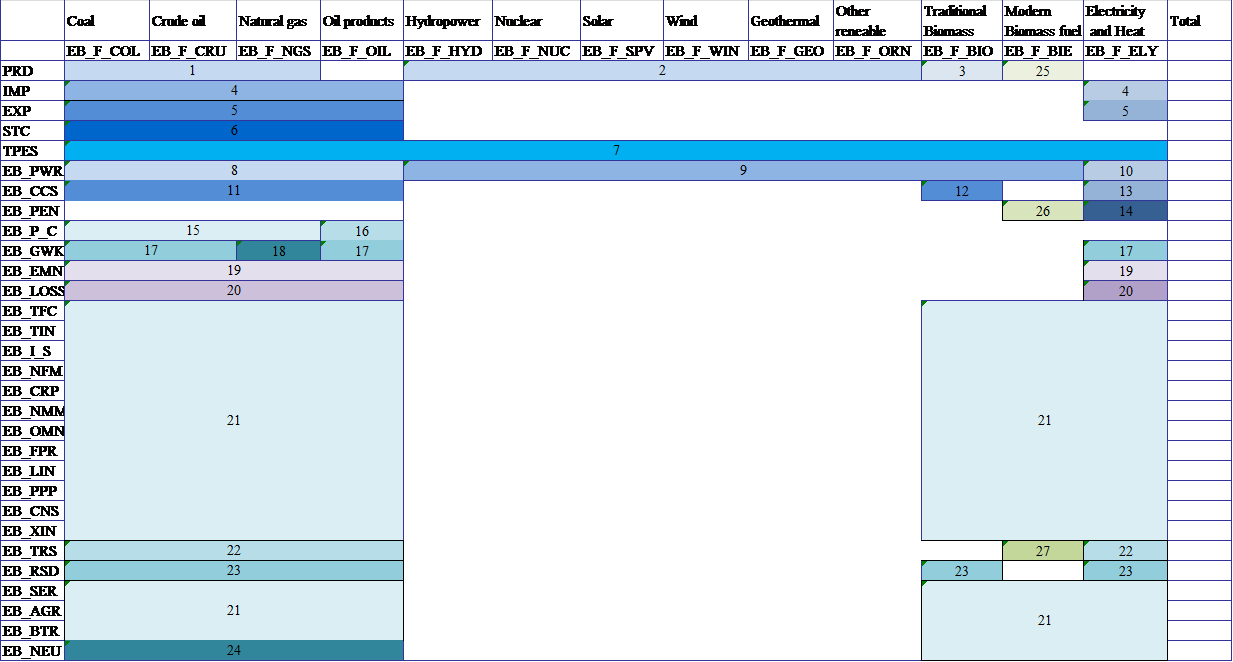
\includegraphics[width=1\textwidth]{fig/image15.png}
\end{table}

\begin{tabularx}{\textwidth}{|
p{\dimexpr 0.104\linewidth-2\tabcolsep-2\arrayrulewidth}|
p{\dimexpr 0.425\linewidth-2\tabcolsep-\arrayrulewidth}|
p{\dimexpr 0.47\linewidth-2\tabcolsep-\arrayrulewidth}|} 
\caption{\label{tab:lisCorEneBalCGE}List of correspondence for energy balance table and CGE model variables} \\
 %------ Top page header ----
 \hline
Cell & Equation (Variable) & Memo \\\hline 
 \endfirsthead
 %------ latter pages header ----
 \multicolumn{3}{l}{\small\it Continued from previous page}\\
 \hline
Cell & Equation (Variable) & Memo \\ 
 \endhead
 %----- latter pages footer --------
 \hline
 \multicolumn{3}{l}{\small\it Continue to next page}\\
 \endfoot
 %----- bottom --------
 \hline
 \multicolumn{3}{l}{\small\it End}\\
 \endlastfoot
\hline 
1 & \-$= QX_{r,c}$ & domestic output of commodity, (Only crude fossil fuel)  \\\hline 
2 & $= QXAC_{r,a''com\_ely''}$ * $ele\_factor_{a}$ & output quantity of electricity of activity a. ''$ele\_factor_{a}$'' is conversion factor; nuclear=3, geothermal=10, biomass=3 \\\hline 
3 & $= QXAC_{r,"bio","com\_ ely"}+\sum _{h}TBH_{r,h}+\sum _{a}TBI_{r,a}$ & Biomass and biomass electricity generation  \\\hline 
4 & = $QM_{r,c}$ & Import quantity of tradable commodity \\\hline 
5 & =- $QE_{r,c}$ & Export quantity of tradable commodity (negative) \\\hline 
6 & = $stck_{r,c}$ & Stock change (exogenous) \\\hline 
7 & =PRD+IMP-EXP+STC & (1+2+3+4+5+6) \\\hline 
8 & $= QINT_{r,c,a}$ & Intermediate inputs of the fossil fuel (only fired- power plants without CCS) \\\hline 
9 & = $QXAC_{r,a,''com\_ely''}$ * $ele\_factor_{a}$ & Output quantity of electricity of activity a. ''$ele\_factor_{a}$'' is conversion factor; nuclear=3, geothermal=10, biomass=3 \\\hline 
10 & $=\sum _{a}QXAC_{r,a,"com\_ ely"}$ & Summation of electricity output (without CCS) \\\hline 
11 & = $QINT_{r,c,a}$ & Intermediate inputs of the fossil fuel (only fired- power plants with CCS) \\\hline 
12 & = $QXAC_{r,a,''com\_ely''}$ * $ele\_factor_{a}$ & Output quantity of electricity of activity a (only biomass). ''$ele\_factor_{a}$'' is conversion factor; biomass=3 \\\hline 
13 & $=\sum _{a}QXAC_{r,a,"com\_ ely"}$ & Summation of electricity output (with CCS) \\\hline 
14 & $=-\sum _{a}QINT_{r,"com\_ ely",a}$ & Electricity consumption by power sectors \\\hline 
15 & = -$QINT_{r,c,''p\_c''}$ & Intermediate inputs of the fossil fuel into petroleum refinery ''P\_C'' \\\hline 
16 & = -$QINT_{r, ''com\_p\_c'', ''p\_c''}$ $+QXAC_{r,''p\_c'',''com\_p\_c''}$ & Output of ''P\_C'' minus input of oil products ''COM\_P\_C'' \\\hline 
17 & =- $QINT_{r,c, ''p\_c''}$ & Intermediate inputs of the fossil fuel of petroleum refinery ''GDT'' \\\hline 
18 & = $QINT_{r,''com\_gas'',''gdt''}$ + $QXAC_{r, ''gdt'',''com\_gdt''}$ & Output of ''COM\_GDT'' minus input of natural gas ''COM\_GAS'' \\\hline 
19 & = -$QINT_{r,c,a}$ & Intermediate inputs of the energy products into fossil fuel mining sector ''COA'', ''OIL'', ''GAS'' \\\hline 
20 & $=-loss_{r,c}(\sum _{a}QXAC_{r,c,a}+QM_{r,c})$ & (Production + import) multiplied by loss rate \\\hline 
21 & $= QINT_{r,c,a}\cdot (1-non\_energy\_rate_{r,c,a})$ & Intermediate inputs of the energy products (excluding non-energy use) \\\hline 
22 & $= QH_{r,c,h}+ QINT_{r,c,''trs''} \cdot road\_rate_{r,c}$ & Transport sector's energy use + household fuel use by car  \\\hline 
23 & $= QH_{r,c,h}- QINT_{r,c,''trs''} \cdot road\_rate_{r,c}$ & household fuel use by car \\\hline 
24 & $= QINT{r,c,a}\cdot non\_energy\_rate_{r,c,a}$ & Intermediate inputs of the energy products multiplied by non-energy use rate \\\hline 
\end{tabularx}

Note:
\begin{enumerate}
\item Export includes international marine and aviation bunkers
\item Oil products includes petroleum products and coal products 
\end{enumerate}

\begin{center}
\begin{tabularx}{\linewidth}{|c|l|l|}
\caption{\label{tab:EneSouMap}Energy source mapping} \\
\hline
energy balance table & energy sources & CGE commodity \\ \hline
EB\_F\_COL & Coa l &COM\_COA \\
EB\_F\_CRU & Crude oil & COM\_OIL \\
EB\_F\_NGS & Natural gas & COM\_GAS \\
EB\_F\_OIL & Oil products & COM\_P\_C \\
EB\_F\_ELY & Electricity and Heat & COM\_ELY \\
EB\_F\_BIO & Modern biofuel & COM\_BIO \\
\hline
\end{tabularx}
\end{center}


\begin{table}
\caption{\label{tab:SecMapTab} Sector mapping table}
\begin{center} 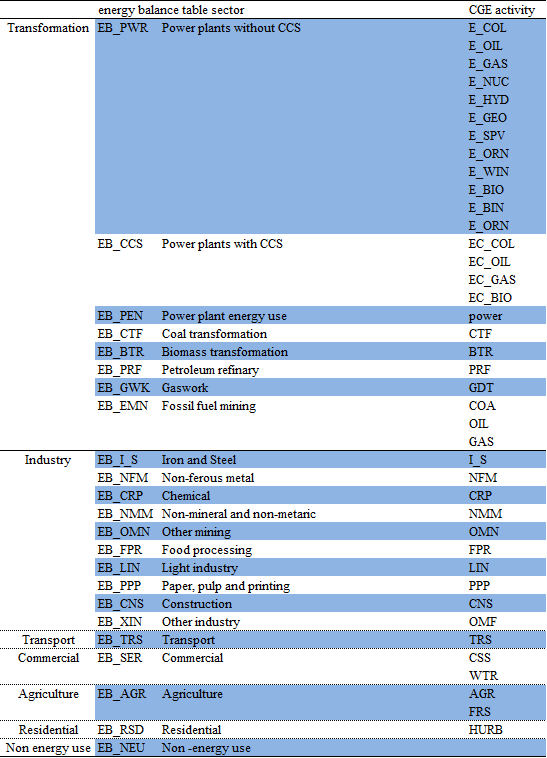
\includegraphics[width=1\textwidth]{fig/image16.png}
\end{center}
\end{table}


\chapter{\label{chp:ChaConExc}Change control excel in \/control\/data\/}

    There is a excel file named as ''excel\_control\_***'' under control folder in in /control/data/. *** should be replaced by the country code. How to use this excel file is described in the readme sheet. Basically, input the scenarios according to the sample data which are already input in this excel file. Then, run the gams file named ''excel\_control.gms''. Finally run the CGE model.  Automatically these sceneario assumptions are loaded.
\begin{itemize}
\item If already the excel exists
\begin{itemize}
\item Add sheet
\item Basically socioeconomic name should be specified as NS1 NS2 and so on. (refer to other sheets)
\item Put explanation and values in it
\end{itemize}

\item If not the excel exists
\begin{itemize}
\item Copy other regions file and name it as the region name
\end{itemize}

\end{itemize}
\section{\label{sec:ReaExcConPro}Read the excel in control program}


\begin{itemize}
\item Modify control/prog/ excel\_control\_new.gms and read the new sheets.
\begin{itemize}
\item Unload the parameter into the gdx which declared in the bottom of the program
\item Add that region code into the loop in control/prog/control\_bat.bat
\item Execute control/prog/control\_bat.bat 
\end{itemize}

\end{itemize}
\section{\label{sec:ReaNatInf}Read the national information}


\begin{itemize}
\item Change /inc\_prog/030\_national\_scenario.gms
\begin{itemize}
\item In order to read the national information, the parameter should be loaded from the control gdx. You can just follow the other examples how they are read.
\end{itemize}

\end{itemize}
\section{\label{sec:MpReaInf}Mapping the read information}

Socioeconomic changes are needed to be configured.

-~/inc\_prog/030\_socioeconomic\_assumption.gms

Add following sentence if the regions are not specified (here is US example)

*----- USA

* National scenarios for United States

* The options are [No, NS1, NS2, NS3 and so on which are defined in the national scenario assumptions]

* The scenarios are specified in cotrol directory.

\$setglobal NS\_USA No

-~/scenario/socioeconomic/\%\%\%.gms

The socioeconomic scenario should include following statement

\$setglobal NS\_USA NS1

-~/inc\_prog/030\_national\_scenario.gms

Add following lines around 150 if the regions are not specified (here is US example)

\seqsplit{\$if not \%NS\_USA\%==No \$batinclude \%prog\_dir\%\textbackslash inc\_prog\textbackslash national\_scenario\_map.gms USA \%NS\_USA\%}

\chapter{\label{chp:GuiChaMod}Guideline for updating the model}

\section{\label{sec:RulWorModPro}Rules for working on the model programing}

Users are classified into three levels.
\begin{itemize}
\item Beginner: can run the model and however, cannot change the code in detail. For example, national model run is made by control sheet shown in section Chapter \ref{chp:HowtoUse}.
\item Code contributor: can run the model, can understand the codes roughly and can modify GAMS codes. 
\item Developer: full understanding of the model and can change model equations and variables.
\item Owner: developer + controls merge branches
\end{itemize}

\subsection{\label{subsec:GitGuid}Git guidelines}

\begin{itemize}
\item Every new work should be done under a new branch.
\item The branch name should be easy to understand but not too long.
\begin{itemize}
\item If the work is under specific project ''Project code''\_''work name''\_''Version name'' (e.g. For suisinhi 2-2002 core scenario work is named as ERF2\_2002\_Core\_V1.0)
\item The project code could be omitted if the work is not under any project. 
\item Similarly the work name could be omitted if the work is obviously only one (like international model inter-comparison project)
\end{itemize}

\item There are three kinds of branches; namely ''master'', ''develop'' and others. 
\begin{itemize}
\item ''master'' is stable and can be used for every project and work. For most of beginners and code contributors are supposed to use this branch as a starting point.
\item ''develop'' is stable and if new model development is needed start from that branch
\end{itemize}

\item Step-by-step guide
\begin{itemize}
\item Create a new branch (see the guide below for how to name your branch)
\item Make your changes
\item Commit your changes (see the advice below for commits)
\item Push your changes (see the advice below for how often to push)
\item When your development is complete, open a pull request.
\end{itemize}

\item General Advice
\begin{itemize}
\item Smaller changes are easier to review. Consider breaking a very large development into several smaller incremental pull requests.
\item Pushing your changes is a way of backing up your work. More frequent pushing is recommended.
\end{itemize}

\end{itemize}
\subsection{\label{subsec:WorRul}Work rule}


\begin{itemize}
\item Beginners are supposed to change socioeconomic, climate policy and impact assumptions.
\item If new assumptions are needed, it is encouraged to add such changes into individual assumptions location.
\item If new assumptions are needed, add lines in the specific location which can be found by searching ''Individual Assumption X'' in prog/scenario.gms.
\item If the assumptions exceeds 30 lines in prog/scenario.gms, it would be recommended to add new sub-program using individual folder.
\item The program owner will consider whether that change should be merged into ''develop'' or ''master'' branches.
\end{itemize}
\section{\label{subsec:CoRul}Code rules}


\begin{itemize}
\item Every equation changes should be noted in this document. The update history also needed to be added.
\item Encouraged to add code notes as much as possible with the reason and purpose of the corresponding changes 
\end{itemize}
\subsection{\label{subsec:TesSceRunAftCodRev}Test scenario run after code revision (for ''develop'' branch) }

After code has been revised and merged into ''develop'', it would be better to test the code for global and national models with default set. To do this, batch/revions\_validation.bat enables to do so. There are three kinds of test
\begin{itemize}
\item Global climate policy variation test under SSP2
\begin{itemize}
\item This process runs BaU, 2.6W 2.0W stabilization and carobn price paths scenarios (in Kriegler et al.~\cite{RN2232}) and INDC\_CONT3 and INDC\_26WCO2.
\end{itemize}

\item Global socioeconomic assumptions variation
\begin{itemize}
\item SSP1, SSP3, SSP4, and SSP5 are run by 26W\_SPA1\_CO2 and 34W\_SPA1\_CO2 of climate policy assumptions 
\end{itemize}

\item National model
\begin{itemize}
\item Japan and China BaU, carbon price paths as mentioned above and 50\% and 70\% GHG emissions reduction compared to 2020.
\end{itemize}

\end{itemize}
\subsection{\label{subsec:ParDec}Parameter declaration (soft) rule}

     Parameter declaration would be better to be ruled in general although there can be many exceptional cases. In /prog/AIMHub.gms process, there is a place where parameters are defined flagged as ''1-3. PARAMETER DECLARATIONS''. There are six classifications on parameter definitions namely;

a. Parameters appearing in model equations  (/inc\_prog/010\_equations.gms)

b. Parameters used for model calibration and scenario assumptions

c. Parameters for variable initialization

d. Parameters for future socioeconomic specifications

e. Results unload parameters

f. Base (year) parameters that are used in the scenarios assumptions but not in the equations

In /prog/scenario.gms, there is a location flagged as ''2-1. MODEL PARAMETERS AND SETS'' where parameters and sets are defined. 

The modelers are encouraged to use above-mentioned spaced to declare the parameters. Note that there are some sub-programs in inc\_prog including parameter declaration. If the parameters are used in the specific file and the number of them are not so large (e.g. less than five), it would be OK to define in those files.

\subsection{\label{subsec:SetDec}Set declaration (soft) rule}

Set is recommended to declared in inc\_prog/010\_setdefine.gms in general.
However, if you would like to add a specific procedure with new inc\_prog files and the usage of the corresponding set is limited to that file, it would be also good to declare in that inc\_prog file.

\section{\label{sec:IncProg}directory Inc\_prog}

In directory ./inc\_prog, file names begin with numbers from 010 to XXX. These numbers indicate as follows:

\begin{itemize}
  \item 010: included in ./prog/AIMHub.gms process 
  \item 020: included in both ./prog/AIMHub.gms and ./prog/scenario.gms processes 
  \item 030: included in ./prog/scenario.gms process
  \item 040: included in ./prog/coombine\_gdx1.gms process
  \item 050: included in ./prog/coombine\_gdx2.gms process
  \item 060: included in other programs
\end{itemize}
  

\section{\label{sec:Deb}Debug}

\subsection{\label{subsec:GenIns}General instruction}

If you can see the ''Normal completion'' in the last part of the window black box or log file (output/log/*), and all the relevant results files are updated, it means you succeeded to run the model. However, if there are any error messages in the window black box or log file (output/log/*), please refer to the .lst file(s) in the {\ldots}/output/lst directory. Please search for error message or ''****'' in these lst file(s) and solve the problem(s).

There are two types of errors; 1)Error without optimization and 2) Optimization is carried out but solution is not found.
\begin{itemize}
\item Optimization is carried out but solution is not found
\item solutionIteration.gms
\begin{itemize}
\item This option cut a year into several pieces by changing the input coefficients changes. Change "maxite".
\item Moreover, if the scenario implements emissions cap but the emissions constraint is too strict to find solution, then this option might solve this problem. This option is to solve the problem tentatively using the same carbon price and then go to the normal solution. Turn on "NoConsSolvFlag2" and change "maxite3".
\end{itemize}

\item Check PA0 (industrial activity price index) which should be normally around 1 but if it is over 10 or less than 0.1, you should suspect very strong constraint forces the corresponding sector.
\item If the log shows like below. The previous iteration results show some inconsistency and check .lst file by searching *****.
\end{itemize}
--- Restarting execution

--- scenario.gms(30722) 289 Mb

--- Reading solution for model STANDCGE

--- scenario.gms(30738) 291 Mb

--- Generating MCP model STANDCGE

--- scenario.gms(30740) 319 Mb 17 Errors

--- LOOPS FOR/WHILE = 1

---   68,919 rows  68,742 columns  341,074 non-zeroes

---   818,836 nl-code  185,365 nl-non-zeroes

--- scenario.gms(30740) 313 Mb

*** SOLVE aborted

--- scenario.gms(30740) 313 Mb 17 Errors

*** Status: Execution error(s)

--- Job scenario.gms Stop 01/22/21 13:58:00 elapsed 0
\begin{description}
\item[Parameter checks]
\item[${\CIRCLE}$]Check the parameters used in the model by turning on the single option on in batch file. Then, check /output/temp/temp2.gdx
\item[${\CIRCLE}$]The base year parameter can be also checked by /output/temp/temp.gdx
\end{description}

\begin{description}
\item[3)]Error without optimization
\item[${\CIRCLE}$]GAMS code error

This can be detected by ''single'' option to stop the simulation at a year
\item[${\CIRCLE}$]GAMS code has no error but the solution does not start

If zero division or equivalent mathematical rule violation, ''single'' option to stop the simulation at a year would help to detect
\item[${\CIRCLE}$]Number of variables and equation differences
\begin{itemize}
\item This would be because wrong assignment and fix or boundary condition of varialbes.
\item If you don't add any equations or variables but see this error, previous year's simulation may have some issue.
\end{itemize}

\item[${\CIRCLE}$]Some examples of errors and notes
\begin{itemize}
\item At the year when new industries or technologies appear, there are high chgance to occur errors. For example, CCS technologies are going into the system (at certain carbon price), advanced biofuel industry gets in 2021, battery technologies are needed at certain share of variable renewable energies.
\item If the equation residuals seem to be difficult to make WMEQ(C) zero, it might be related to the international transport fuel usages.
\item 
\end{itemize}

\end{description}
\subsection{\label{subsec:SomSpeErr}Some specific error examapls}

1)~Unsolved with iteration in residual of WMEQ(''COM\_P\_P'')\}

  The international trade fuel consumption exceeds the potential export of ''COM\_P\_P''. Review the assumptions on international transport energy consumption.

(Update in Nov., 2021)

This repsentation has changed and no longer related.

2)~CCS related equations residual\label{mark-2)}

  Carbon price goes down and then some variables related to CCS reached to zero and cause errors.

\section{\label{sec:AddNewEquVar}Add new equations and variables}

This section describes the procedure how to add new equations and variables into the CGE model. Since the model is on the MCP basis and initial, lower boundary, upper bounary values, or fixing conditions are needed to be specified and several steps are required. To do this, Cygwin must be installed.

\begin{landscape}
\begin{tabularx}{\textwidth}{|
p{\dimexpr 0.061\linewidth-2\tabcolsep-2\arrayrulewidth}|
p{\dimexpr 0.30\linewidth-2\tabcolsep-2\arrayrulewidth}|
p{\dimexpr 0.591\linewidth-2\tabcolsep-2\arrayrulewidth}|} 
\caption{\label{tab:ProAddNewEqu}Procedures to add new equations and variables} \\
 %------ Top page header ----
 \hline
Num. & Procedure & Descritpion \\\hline 
 \endfirsthead
 %------ latter pages header ----
 \multicolumn{3}{l}{\small\it Continued from previous page}\\
 \hline
Num. & Procedure & Descritpion \\ 
 \endhead
 %----- latter pages footer --------
 \hline
 \multicolumn{3}{l}{\small\it Continue to next page}\\
 \endfoot
 %----- bottom --------
 \hline
 \multicolumn{3}{l}{\small\it End}\\
 \endlastfoot
\hline 
(1) & Write the equations  & /inc\_prog/010\_euqations.gms \newline POWER\_SHARE\_AGG\_LOW(Ragg,Aagg)\$(power\_share\_agg\_lo(Ragg,Aagg)).. \newline
0 =G= (power\_share\_agg\_lo(Ragg,Agg)*SUM(AP\$(theta(R,AP,"COM\_ELY")), \newline theta(R,AP,"COM\_ELY")*QA(R,AP))-SUM(R\$Map\_Ragg(R,Ragg), SUM(A\$Map\_Aagg(A,Aagg), theta(R,A,"COM\_ELY")*QA(R,A))));  \\\hline 
(2) & Declaration of variable and equation, related parameters and specification of attribution of variables, load and unload results. \newline This procedure automatically made by the program modification tool. & Execute /tool/prog\_mod/prog/var\_add.sh (1) \newline Variable and equation name, elements and description should be specified in /tool/prog\_mod/data/varset.data and /tool/prog\_mod/data/equset.data. The orders are name, elements and description.  \newline Then execute bash copy\_mod.sh (2) \newline POWER\_SHARE\_AGG\_LOW Ragg,Aagg Lower boundary of renewable energy group \newline VRENSHR\_AGG Ragg,Aagg Dummy variable for renewable power generation group share \\\hline 
(3) & If you need complementary condition, add the complementary variables to equations. & /inc\_prog/010\_model\_dec.gms \newline ''POWER\_SHARE\_LOW.VRENSHR   '' \newline POWER\_SHARE\_AGG\_LOW.VRENSHR\_AGG \\\hline 
(4) & Define and take differences of each equation. \newline The equation name is already written in the program after you execute procedure (2). Thus find the location by searching ''add\_equ\_loc\_2'' and specify the difference. & /inc\_prog/030\_check\_infes.gms \newline POWER\_SHARE\_LOW0(R,A)\$(ACT0(R,A) AND power\_share\_lo(R,A)) (power\_share\_lo(R,A)*SUM(AP\$(theta(R,AP,"COM\_ELY")), theta(R,AP,"COM\_ELY")*QA0(R,AP)) - theta(R,A,"COM\_ELY")*QA0(R,A))= 0; \newline 
POWER\_SHARE\_AGG\_LOW0(Ragg,Aagg)\$(power\_share\_agg\_lo(Ragg,Aagg)) = (power\_share\_agg\_lo(Ragg,Agg) * SUM(AP\$(theta(R,AP,"COM\_ELY")), theta(R,AP,"COM\_ELY") * QA00(R,AP))-
SUM(R\$Map\_Ragg(R,Ragg), SUM(A\$Map\_Aagg(A,Aagg), theta(R,A,"COM\_ELY") * QA00(R,A)))); \\\hline 
(5) & Scale the equations. The equation name is already written in the program after you execute procedure (2). Thus find the location by searching ''add\_equ\_loc\_1'' and specify the scaling parameter. & /inc\_prog/020\_scale\_global.gms \newline POWER\_SHARE\_LO.SCALE(R,A)\$(ACT(R,A) AND power\_share\_lo(R,A) AND theta(R,A,"COM\_ELY")*QA.L(R,A)) = \newline
SQRT(ABS(theta(R,A,"COM\_ELY")*QA.L(R,A))); \newline
 POWER\_SHARE\_AGG\_LOW.SCALE(Ragg,Aagg)\$(power\_share\_agg\_lo(Ragg,Aagg) AND \newline
(SUM(R\$Map\_Ragg(R,Ragg), SUM(A\$Map\_Aagg(A,Aagg), theta(R,A,"COM\_ELY") * QA.L(R,A)))))= 
SQRT(ABS(SUM(R\$Map\_Ragg(R,Ragg), SUM(A\$Map\_Aagg(A,Aagg), theta(R,A,"COM\_ELY") * QA.L(R,A))))); \\\hline 
(6) & If you need lower boundaries, put them. & /inc\_prog/BaseScenarioBoth/lower.inc \newline   VRENSHR.LO(R,A)\$(power\_share\_lo(R,A)) = 0 ; \newline   VRENSHR\_AGG.LO(Ragg,Aagg)\$(power\_share\_agg\_lo(Ragg,Aagg))= 0 ; \\\hline 
(7) & Through the calibration procedure you need to specify the initial parameters like (VARNAME0) & /inc\_prog/010\_calibration.gms \newline   power\_share\_lo(R,A) = 0 ; \newline   VRENSHR0(R,A) = 0 ; \newline   power\_share\_agg\_lo(Ragg,Aagg)=0; \newline   VRENSHR\_AGG0(Ragg,Aagg) = 0 ; \\\hline 
(8) & Set the parameters for new renewable energy and CCS technology & /inc\_prog/030\_CCS\_industry.gms \newline /inc\_prog/030\_renew\_production\_calib.gms \newline /inc\_prog/030\_renew\_prodcution.gms \\\hline 
(9) & VARFIX.gms & VRENCAP.FX(R,A)\$(NOT (QA.l(R,A) AND (Prenew\_up(R,A) OR power\_share\_up(R,A) OR prodscenario(R,A))))=0; \newline VRENSHR\_AGG.FX(Ragg,Aagg)\$(NOT (power\_share\_agg\_lo(Ragg,Aagg) AND SUM(R\$(Map\_Ragg(R,Ragg)),SUM(A\$(Map\_Aagg(A,Aagg)),QA00(R,A)))))=0; \\\hline 
(10) & Declare parameter & AIMHub.gms \newline power\_share\_lo(R,A)   Power share lower boundary \newline  power\_share\_agg\_lo(Ragg,Aagg)   Power group share lower boundary \\\hline 
(11) & Modify income equation &  Equations.gms \newline                -QA(R,A)*VRENSHR(R,A) \newline           VRENCAPTOT(R,INSDNG) =E= SUM(A,QA(R,A)*(VRENCAP(R,A)-VRENSHR(R,A)))*shincome(R,INSDNG); \newline     VRENCAPTOT(R,INSDNG) =E= SUM(A,QA(R,A)*(VRENCAP(R,A)-VRENSHR(R,A)-SUM(Ragg\$Map\_Ragg(R,Ragg),SUM(Aagg\$Map\_Aagg(A,Aagg), VRENSHR\_AGG(Ragg,Aagg)))))*shincome(R,INSDNG); \\\hline 
\end{tabularx}
\end{landscape}

\section{\label{sec:HowAddSec}How to add sectors}

This section describes how to add hydrogen production sectors. This procedure can be adopted to any other sector introduction. 
For example, introduction of artificial meat production sector has been made under the commit number  "ed2f31d"  in AIMHub repository and you can refer how it has been realized by looking at this commit.
Another example is introduction of enhanced weathering commit number "c7bee8e" in AIMHub repository and you can refer how it has been realized by looking at this commit.
Further example is introduction of soil carbon and biochar commit number "71d9d1" in AIMHub repository and you can refer how it has been realized by looking at this commit.


\subsection{\label{subsec:ProNonEleSec}Procedure for non-elecrticity sector}

Assume that now hydrogen sector is to be added.
\begin{itemize}
\item HGC
\begin{itemize}
\item Set map file change or add

\item /Define/activity.set
      HGC Hydrogen by coal
      HGG Hydrogen by gas
      HGB Hydrogen by biomass
      HGE Hydrogen by electricity
\end{itemize}

\item COM\_HYG
\item ~/Define/commodity.set
\begin{itemize}
\item /Define/ household\_commodity.set
\item /Define/ householdc.map
\end{itemize}
COM\_ENE . COM\_HYG
COM\_CAR . COM\_HYG
\end{itemize}

\begin{description}
\item[1)]New program for generating the sectors
\item[-]Copy from ./inc\_prog/030\_biofuel.gms to ./inc\_prog/030\_hydrogen.gms
\item[-]Need to be declared
\begin{itemize}
\item \textcolor{color-3}{A\_HYG(A)}
\item \textcolor{color-3}{C\_HYG(C)}
\item Hyginirate(R,A)
\item Hyginidemand(R,A)
\item hydinirate(R)
\end{itemize}

Demand side specification should be made in ./inc\_prog/030\_NewIndsutryCalib.gms.

\subsection{\label{subsec:ElecSecCas}Electricity sector case}

\end{description}
Assume that E\_WIF is to be added to an electricity sectory.
\begin{itemize}
\item Search from all ''E\_WIN''
\item Inc\_prog/Combine\_gdx.gms
\begin{itemize}
\item Add ''E\_WIF'' to a Set DUM
\item Newly declare A\_WIF(A) to /inc\_prog/010\_data\_import.gms.
\item Add A\_WIF to gdx/set.gdx
\end{itemize}

\item prog/Combine\_gdx2.gms
\begin{itemize}
\item Add ''E\_WIF'' to a Set DUM
\item Search WIN  and add W\_WIF where WIN is found.
\item Add WIF in a set of ''Fuel''
\end{itemize}

\item Calibration.gms, Data\_import.gms, Ene\_bal\_make.gms
\begin{itemize}
\item Search Win and add WIF where Win is found.
\end{itemize}

\item Renew\_production.gms
\begin{itemize}
\item Supply curve and potential is set in scenario\_parameter.gms.
\item Input coefficient is assumed same as E\_WIN.
\end{itemize}

\end{itemize}


Moreover, for the reporting of the results, multiple locations should be reviewed.
\begin{itemize}
  \item ./prog/combine\_gdx1.gms
  sector mapping allocation such as Msec(AC,Ssec), Mene\_S\_FC(ENE\_S,AC), and Msec(AC,Ssec) should add sectors.
  \item ./inc\_prog/040\_ene\_bal\_make.gms
  if the newly added sector is not normal final energy consumption sectors such as energy transformation, then there should be some specifial treatment to generate energy balance table. 
\end{itemize}


\subsection{\label{subsec:EssPro}Emissions specificiation if the sector exists in base year SAM}

\begin{itemize}
\item If the sector is existing in the base year, it should be mapped to EDGAR emissions
\begin{itemize}
\item Using excel file
\item Modification of mapping in Data/edgar/emission.xls
\item Execution of emission.gms
\end{itemize}

\item Execution of ./data/AIMHubdata/elasticity/elasticity\_set.gms
\item Execution of AIDADS\_para.gms
\end{itemize}


\section{\label{sec:HowAddAnaVarFinRes}How to add analytical variables to the final results or figures}


\begin{itemize}
\item This section describes how to add analytical variables to the final results or figures.
\item The main task is interpretation of CGE variables to the final indicator format
\end{itemize}
\subsection{\label{subsec:Com1}Combine\_gdx1.gms}


\begin{itemize}
\item This program combines all years information for a particular scenario. You should add one parameter in combine\_gdx1.gdx. Let us assume parameter XXX is supposed to be added.
\begin{itemize}
\item XXX is corresponding to CGE model results. 
\end{itemize}

\item Extract CGE model results 
\begin{itemize}
\item Find the words ''LOAD CGE DIRECT RESULTS'' and then you see the list of parameter declaration and GDX loading.
\item You should declare parameter which you want to include for XXX
\item Then, write that parameter after \seqsplit{\$gdxin '\%output\_dir\%/\%file\_loc\%/cbnal0/\%region\%\_\%SCENAME\%\_\%CLP\%.gdx}
\end{itemize}

\item Regional aggregation
\begin{itemize}
\item It is normally 17 regions information, thus to extract regionally aggregated results we put aggregation equation.
\item Find ''REGIONAL AGGREGATION'', then you find the examples how to aggregate them.
\end{itemize}

\item Compute indicators
\begin{itemize}
\item Find ''COMPUTE INDICATORS''
\item After that write down the equation
\end{itemize}

\item Store the results into GDX file
\begin{itemize}
\item Find ''UNLOAD COMPUTED INDICATORS'', then you see the GDX unload command and indicators are stored into \%output\_dir\%/\%file\_loc\%/cbnal /\%SCENAME\%\_\%CLP\%.gdx
\item Put your indicator parameter name into that.
\end{itemize}

\end{itemize}
\subsection{\label{subsec:Combine2}Combine\_gdx2.gms}


\begin{itemize}
\item This program combines all scenario results as one database. You should add again the parameter.
\item Load indicators which you have stored in combine\_gdx1.gms
\begin{itemize}
\item Find ''LOAD INDICATORS'' and then put the parameter which you have stored. Before that, you also need to declare the parameter.
\item Be cautious that the parameter needs to have scenario dimensions (see other examples)
\end{itemize}

\end{itemize}
\subsection{\label{subsec:IAMCTemSts}IAMC template system }

  This procedure is supposed to follow the document which is in the tools/iiasa\_database
To participate international model inter-comparison projects like EMF, 
the data submission form is mostly harmonized to IAMC data template system. 
This tool aims to make such data submission form by using AIM/Hub results.
\\
  Mapping the results of AIM/CGE. Regions, variables, scenario names and units. 
The input data is main indicators of AIM/Hub results which include emissions, energy, agriculture and land use. 
Through the process simplified climate model MAGICC is run. In linux system including WSL, MAGICC7 is run and in cygwin system, MAGICC6 is run.
This procedure is run if the swtich of "database" is turned on in the main shell control file.
\\
  When you want to add scenario names and mapping with them, use /define/scenario.set and /define/scenario.map. 
The former file is for declaration of scenario name and the latter is for the mapping. 
For instance, suppose that you are asked to submit a scenario named "SSP2\_Ref\_SPA0" which corresponds to the scenario "SSP2\_BaU\_NoCC" in your model running, and
then, /define/scenario.set should have "SSP2\_Ref\_SPA0" and /define/scenario.map should have the following maping.
\\
SSP2\_BaU . SSP2\_Ref\_SPA0
\\

For each exercise, variable list can change, and in such cases, we must specify the variables which should be eliminated from this data submissions. 
First, you copy the variable list from the shared variable list and paste into the excel sheet "template\_sheet" in "variable\_list\_IAMC.xlsx" (column B). 
Then you have a list of code which should be included in the output column C ( rest of them are excluded from the list). 
Copy the list into /data/include\_parameter.txt

  The file location of the output is /output/iiasa\_database/gdx/global\_17\_IAMC.gdx or /output/iiasa\_database/txt/global\_17\_IAMC.csv.
Individual scenario gdx files are also located in /output/iiasa\_database/scenario.

\subsubsection{\label{subsubsec:HowtoAddVar}How to add variables?}

\begin{itemize}
\item update and get latest IAMC template repository (\url{https://github.com/KUAtmos/IAMCVariableChange}) and see IAMCTemplate.txt
\item Add variable names, codes, units and relevant information
\item	This IAMCTemplate.txt should be fully copied into the spread sheet of /doc/Variable\_List\_IAMC.xlsx TemplateRepo (column A to N)
\item	Add weighting variables for regional aggregatoin in the sheet "master" column J.
\item	List up variables which have aggregation relationships and write down in "aggregation" sheet in /doc/Variable\_List\_IAMC.xlsx. The column B should have aggregated variables and the column C should have disaggregated variables. 
\item	Copy the contents of column E to G to define/aggregation.map.
\item	Write programing codes in prog/iiasa\_database\_ind.gms to speciffy the variables. In this process, the output results of CGE are allocated to the parameter named EMFtemp1. In this program, aggregated variables which are already specified in the previous steps don't need to be written.
\item	if the corresponding vairiables are economic indicators that should be deflated by price index (mainly for 2005 to 2010US dollar), 
add the varialbe into tools/iiasa\_database/define/EconomicInd.set or EconomicInd\_Price.set
\end{itemize}


\section{\label{sec:NotTooDir}Note of tools directories - analytical tools management}

This section summarizes how to manage analytical tools for CGE model results. CGE analytical tools are managed by subversion in ./tools. There are for example simplified climate model, IIASA database submission form tool and so on.

\subsection{\label{subsec:BasIde}Basic idea}


\begin{itemize}
\item The analysis using AIM/CGE should be made under /tools directory. It is beneficial for all CGE users since we can share the analytical tool and treat them separately from CGE main body.
\item Creating directory under /tools and put programs, maps and data files.
\item The output or temporary files of the analytical tools should be stored in /output which is same hierarchical directory as /tools. Basically making directory for that analysis is recommended.
\begin{itemize}
\item For example, output/iiasa\_database is made under the process of IIASA database submissions tool.
\end{itemize}

\item The execution of the analysis should be managed under bat or shell files. The example can be seen under tools/iiasa\_database/prog.
\begin{itemize}
\item The batch or shell file should include making directory also.
\end{itemize}

\item GAMS execution of this analysis is highly encouraged to do under /exe directory which is located same hierarchical directory as /tools. It is because GAMS execution creates many dump files and to keep the directory clean.
\item The user must remain a ''read me'' file for the analysis under the folder (see example in /iiasa\_data\_submission/readne.docx.)  or directly describe in this documentation. 
\end{itemize}
\subsection{\label{subsec:ReaMeExa}Read me example}


\begin{tabularx}{\textwidth}{|
p{\dimexpr 0.165\linewidth-2\tabcolsep-2\arrayrulewidth}|
p{\dimexpr 0.835\linewidth-2\tabcolsep-\arrayrulewidth}|} 
\caption{\label{tab:ReaExaIAMC}readme example for IAMC database template} \\
\hline 
Name & A tool for IIASA Database submission form  \\\hline 
Introduction & Participating international model inter-comparison projects like EMF and SSP, the data submission form is mostly harmonized to IIASA data system. This tool aims to make such data submission form by using AIM/CGE results. \\\hline 
Method & Mapping the results of AIM/CGE. Regions, variables, scenario names and units. The input data is main indicators of AIM/CGE results which include emissions, energy, agriculture and land use. The output is data submission form. Through the process simplified climate model MAGICC is run. \\\hline 
Main program directory & /Tools/iiasa\_data\_submission \\\hline 
Execution file & /Tools/iiasa\_data\_submission/prog/iiasa\_database.bat \\\hline 
Input file & combine\_gdx2 process which is temporarily saved by SAVE command is restarted. Therefore, all information created by /prog/prog/combine\_gdx2.gms process is the input. \\\hline 
\end{tabularx}

\begin{tabularx}{\textwidth}{|
p{\dimexpr 0.165\linewidth-2\tabcolsep-2\arrayrulewidth}|
p{\dimexpr 0.835\linewidth-2\tabcolsep-\arrayrulewidth}|} \caption{\label{tab:ReaExaMAGIC}readme example for MAGICC}\\
\hline 
Name & MAGICC (simplified climate model \\\hline 
Introduction & We are sometimes required to submit or show climate information which is associated with particular emissions scenarios. This tool is for generating such information. If you use Cygwin, MAGICC6 is used and otherwise MAGICC7 is used. \\\hline 
Method & Preparing emissions data from AIM/CGE and running MAGICC which is publically available. \\\hline 
Main program directory & /Tools/MAGICC. MAGICC itself is located under the directory / MAGICC/MAGICC6\_4Download and the data processing is made by the programs in / MAGICC/CGE2MAGICC \\\hline 
Execution file & /Tools// MAGICC/CGE2MAGICC/cge2magicc.bat \\\hline 
Input file & Output/global/global\_17/gdx/emissions.gdx. this file includes emissions scenarios. Other emissions that are not covered by AIMHub is interpolated from CMIP6 ScenarioMIP data which is stored in original MAGICC7.
This can be specified by the file /tools/magicc/CGE2magicc7/data/OtherGasMap.txt. This text file needs to specify scenario names and other gas emissions mapping by using tab separated format. 
Default is SSP2-4.5W scenario.\\\hline 
Output file & The output file is gdx file named as /output/magic/iiasa\_database\_climate.gdx \\\hline 
Other considerations & This tool can be run under IIASA database submission form tool. \\\hline 
Output file & The output file is the text file for submissions located as /output/iiasa\_database/ iiasa\_database\_final.txt. \\\hline 
Other considerations & Some variables are not allowed to submit for some projects, in such cases we must specify the variables which should be eliminated from this data submissions. Those variables should be written in /tools/iiasa\_data\_submission/data/eliminates.txt \\\hline 
\end{tabularx}

\chapter{\label{chp:TipsMIP}Tips for MIP participations}

\section{\label{sec:DefNewSce}Defining new scenarios}


\begin{itemize}
\item Judge whether the exercise requires new socioeconomic assumptions or climate policy assumptions
\begin{itemize}
\item The socioeconomic assumption revision is needed for assuming the demographic, economic, technological and other resource aspects.
\item Climate assumption usually changes the climate target, emissions pathways and carbon price paths and so on.
\end{itemize}

\end{itemize}
\section{\label{sec:SomeTIPS-SocAss}Socioeconomic assumption}


\begin{itemize}
\item Add new socioeconomic assumptions in prog/prog/scenario/socioeconomic/
\begin{itemize}
\item Usually copy SSP2 and rename it.
\item Then, specify each exercise assumptions. The specification would potentially be in various files.

\item If you need to change the parameters (not model structure), usually you just change the prog/scenario.gms or prog/inc\_prog/020\_socioeconomic\_assumption.gms
\end{itemize}

\end{itemize}
\section{\label{sec:AddVarIIADatSys}Adding variables to the IIASA data system}

1)~List up the variables which have not used earlier in the CGE system but newly required.\label{mark-1)}

Using vlookup function in excel is useful for this procedure.

Then, add them into the excel file (/doc/variable\_list\_IAMC.xlsx map)
\begin{description}
\item[2)]Scenario name defining and mapping
\item[-]iiasadatabase/define/scenario.set
\item[-]iiasadatabase/define/scenario.map
\end{description}

\begin{description}
\item[3)]include parameters
\item[-]you should specify the variables list for the submission in the \seqsplit{iiasa\_database/define/include\_parameter.set}
\item[-]This can be done by using the third sheet in /doc/variable\_list\_IAMC.xlsx
\end{description}
\chapter{\label{chp:ModFea}{Model features}}
\footnote{Parts of this section may overlap with other sections.}\label{mark-11.}
This chapter documents a main model structure and how to implement scenario assumptions for the analysis of long-term climate mitigation taken by AIM/Hub. 
There are six aspects which are going to be discussed. First, macro economy, labor and population treatment are explained. Second, energy supply sectors representation is described. 
Energy supply sectors are one of the key elements for decarbonizing economic systems. 
Thrid, energy demand sectors are discussed. 
Forth, agrilture and land use is critically important for stringent climate mitigation policy since large bioenergy implementation combined with carbn capture and storge, and afforestation would be thought as measures which enales so-called negative emissions. 
Fifth, non-energy realted GHG reduction measures follow. They are mostly related to agricultrural sectors. 
Sixth, we discuss how to add new sectors into the CGE system.

\section{\label{sec:SomTIPS-Int}{Introduction}}

This section documents a main model structure and how to implement scenario assumptions for the analysis of long-term climate mitigation taken by AIM/CGE V2.0 (we call AIM/CGE from here). AIM/CGE is a multi-region and multi-sectors recursive dynamic type CGE model. There are several features to understand the behaviors of this model in conjunction with future scenarios. There are six topics as follows and they will be explained by each section later.
\begin{enumerate}[{1)}]
\item {Macroeconomic, labor, population}
\item {Energy supply}
\item {Energy demand} 
\item {Agriculture and land use}
\item {GHG reduction measures other than changing energy system}
\item {How to implement new production sectors or goods (not accounted in the base year)}
\end{enumerate}
{In this document, we put much more priority on showing how the scenario outcomes of this model are generated than just explaining either model structure or scenario assumptions. We keep a basic rule that each section provides following structure as much as possible.}
\begin{itemize}
\item  {The importance of the factors}
\item  {The fundamental logics of the basic model structure} 
\item  {How the exogenous assumptions are fed into the model for future simulations}
\item  {Actual parameter settings}
\item  {Limitation and remained issues that should be improved further version.}
\end{itemize}
\section{\label{sec:DemMacCha}Demographic and macroeconomic change }

\subsection{\label{subsec:PopLabPar}Population and labor participation}

Future demographic change is one of the key drivers to change the future goods demand including energy and food. On the other hand, the production side is also affected by the demographic change through labor participation.

The population and labor forces are exogenous parameters for AIM/CGE. The macroeconomic growth is also the exogenous assumption.

The first-order effect of population change is the household consumption. The household consumption is formulated as LES (Linear Expenditure System) and it consists of two factors for each commodity consumption; namely subsistence consumption and marginal share of consumption. The population change directly effects on the former factor.

The population increase ratio relative to previous year is multiplied to the subsistence consumption parameter $\beta _{r,ch,h}^{m}$. The latter factor, marginal share of consumption, specifies how the household money excluding subsistence consumption is spent and the expenditure share of each commodity is determined. Thus, it is not directly influenced by the population change. The intermediate inputs of agricultural commodity are also associated with population change.

There might be a discussion about the assumption in fixing population. The population and labor force could be affected by the future climate change impact through change of health condition including change of agricultural goods availability or migration induced by the environmental change. We ignore basically in the mitigation analysis. The exception can be seen in the study highlighting climate change impact (Hasegawa et al. 2016).

\subsection{\label{subsec:MacCha}{Macroeconomic change}}

Future macro-economic assumption also causes goods demand and supply. The macroeconomic growth is also the exogenous assumption. Usually the GDP change is used for the macroeconomic assumption for the Integrated Assessment Models' (IAMs) future scenario simulation. However, the actual outcome from the model is not exactly same as the assumptions. Therefore, the GDP assumption is used for calculating total factor productivity (TFP) and TFP is totally exogenous parameter for the model.

The economic growth is realized by three factors: labor force change, accumulated capital and total factor of productivity. The labor force is the one of the three main drivers of the GDP. The labor force change is exogenous variable for this model. The production sectors are basically \footnote{Power sectors have different structure as shown in the formula} assumed to have multi nested CES (Constant Elasticity of Substitution) function. Therefore, if the labor wage is constant, labor force change ratio is directly affects to the GDP change.

The GDP assumptions for the future scenarios are used in the scenario analysis while GDP is endogenously determined in the CGE model. As is mentioned previously, economic growth is realized by labor force, capital and TFP. Thus, there are four degree of freedom. Labor is exogenous as indicated previously. Total capital accumulation is also determined a priori for a year since the total capital which is able to participate in production is previous year's capital formulation plus accumulation with certain of depreciation. Then, TFP is an unknown parameter. We use the GDP assumptions to calculate TFP change.

Let the total labor, capital and GDP be given and the Hicks-neutral technical change is assumed. Then, the TFP annual change is determined as below.
\begin{equation}
\tag{2}
GDP_{r}=tfp_{r}\cdot F\left(K_{r},L_{r}\right)\,,\forall r\in R
\end{equation}
{Where} 

$tfp_{r}$  : TFP change ratio to previous year in region r,

$gdp_{r}$  : expected GDP assumptions in region r,

$L_{r}$  : Total labor participation in region r,

$K_{r}$  : Total accumulated capital in region r.

The CES function is used for the function F. The TFP change ratio derived from the above equation is multiplied to the all sectors. This TFP change calculation is made only for the scenario excluding climate mitigation (what we call BaU scenario) and the scenarios with climate change mitigation adopt the BaU scenario's TFP change under same socioeconomic assumptions.

\section{\label{sec:EneSup}{Energy supply}}

The energy supply is classified into three parts. They are fossil fuel extraction, bioenergy supply, power supply including renewable energy. These energy supply sectors play a key role to determine the future carbon price under climate mitigation scenarios. The current amount of CO2 emission itself from power sectors is relatively larger than other sectors and this sector has large potential to reduce the emissions.

\subsection{\label{subsec:FosFueExt}Fossil fuel extraction}

Fossil fuel extraction costs are projected to increase in the future in line with the current situation. This is mainly due to the limitation of cheap fossil fuel resource reserves and the increase in demand.

There are three fossil fuel extraction sectors within this CGE model; namely coal, crude oil and natural gas. The cost of fossil fuel mining is determined by the assumptions of those sectors' production function. The production structure is as shown below. This structure is assumed for other sectors excluding energy transformation sectors.

Each producer (represented by an activity) is assumed to maximize profits, defined as the difference between revenue earned and the cost of factors and intermediate inputs. Profits are maximized subject to a production technology, the structure of which is shown in Figure 4. At the top level, there is non-energy related GHG emission and conventional inputs. Conventional inputs technology is specified by a Leontief function of the quantities of energy, value-added, aggregate non-energy intermediate input and resource input.

The model calculates the extraction cost curve using Rogner (1997) and U.S. Geological Survey (2000), and accordingly the production costs increase by region and fuel. We calculate cumulative fuel extraction every year in recursive iterations. The input of the fossil fuel sector is thought to increase based on the extraction cost curve. All inputs coefficients associated with production function are assumed to be increased according to the extraction cost curve \footnote{To avoid drastic change of the price, we put maximum annual change ratio as 5\%.}. 

\subsection{\label{subsec:FosFueExt-PowGen}Power generation}

Given the electricity demand, the technological share (e.g. Conventional fossil fuel fired, solar, wind and so on) is determined by the power generation prices of each technology. A logit function is used for this selection. The power generation prices for each technology are determined by each production function.

There are two parameters in the equation. The exponent of the logit is exogenously determined for not only future scenario simulation, but also the calibration procedure and we tentatively use the value 2.

The other parameter appeared in the equation is share parameter for each power generation. That parameter is basically calibrated in the base year. The calibrated share parameter can be interpreted as the representation of preference, political decision or the results of any factors other than cost. In the future simulation, we need to update this parameter since the currently unused or less used technologies such as renewable technologies are not appropriately represented in base year's share parameter. Therefore, we assumed that at a certain year the sum of share parameters for the renewable technologies (wind, solar and biomass) supposed to have same share as fossil fired power and the same values are shared by the renewable technologies (if the fired power share parameter is 1, the wind, solar and biomass have 0.33 for each) \footnote{Thus, this approach has an advantage to foresee long-term future share of the technologies but near-term forecast would not be relatively good at.}. The year which has above treatment is tentatively 2050. To realize the objective parameters, we update the parameters with annual constant ratios for each technology.

The price of electricity generated by renewable energy source is assumed to be declined in the future. The future technological cost of renewable energy is uncertain. Hence, we follow the assumptions of Energy Technology Perspective (IEA 2012) for the reference. The input coefficients of intermediate goods and production factors in renewable energy sectors are changed overtime according to the (IEA 2012)'s perspective. Power sector is disaggregated in detailed as mentioned previously. Solar, wind, biomass and geothermal energy power generation are included as renewable energy sources. The actual assumptions used in the model are shown in Table \ref{tab:CapFac} to Table \ref{tab:CostShareTra}. The expected output price of each technology in 2050 is calculated based on these assumptions. The input coefficients of those sectors are assumed to be changed with constant ratio through 2050. This ratio is computed from the cost of base year and shown in the Tables. The conventional fossil fired power is assumed to have annual 0.5\% improvement for the entire period. Note that considering variations in capacity factor of variable renewable energy, we use AIM/Technology's output as \ref{tab:CapFacReg}.

{The return of the capital should have two components; namly pure investment return without profit and profit (premium) parts. For the former one, we calculate the base year capital return ratio (\$) to capacity expressed by physical GW by assuming all vitages are equally accumulated meaning that depreciation of 4\% is assumed to the old capital and add up for life time. The profit part is quite uncertainty which would also be dependent on the countries' general interest rates. Here it would be difficult to identify the rates and thus we assume annual 3\%. Then, we apply the capital return for the future scenarios.}


\begin{tabularx}{\textwidth}{|
p{\dimexpr 0.167\linewidth-2\tabcolsep-2\arrayrulewidth}|
p{\dimexpr 0.167\linewidth-2\tabcolsep-\arrayrulewidth}|
p{\dimexpr 0.167\linewidth-2\tabcolsep-\arrayrulewidth}|
p{\dimexpr 0.167\linewidth-2\tabcolsep-\arrayrulewidth}|
p{\dimexpr 0.167\linewidth-2\tabcolsep-\arrayrulewidth}|
p{\dimexpr 0.167\linewidth-2\tabcolsep-\arrayrulewidth}|} 
\caption{\label{tab:CapFac}Capacity factor (\%)}\\
\hline 
  & 2010 & 2020 & 2030 & 2040 & 2050 \\\hline 
E\_COL & 85 & 85 & 85 & 85 & 85 \\\hline 
E\_GAS & 85 & 85 & 85 & 85 & 85 \\\hline 
E\_OIL & 85 & 85 & 85 & 85 & 85 \\\hline 
E\_HYD & 40 & 40 & 40 & 40 & 40 \\\hline 
E\_NUC & 85 & 85 & 85 & 85 & 85 \\\hline 
E\_SPV & 18 & 19 & 20 & 20.5 & 21 \\\hline 
E\_WIN & 30 & 32.1 & 34.3 & 35.5 & 36.8 \\\hline 
E\_GEO & 70 & 70 & 70 & 70 & 70 \\\hline 
E\_BIO & 85 & 85 & 85 & 85 & 85 \\\hline 
E\_ORN & 70 & 70 & 70 & 70 & 70 \\\hline 
E\_BIN & 85 & 85 & 85 & 85 & 85 \\\hline 
\end{tabularx}

\begin{tabularx}{\textwidth}{|
p{\dimexpr 0.167\linewidth-2\tabcolsep-2\arrayrulewidth}|
p{\dimexpr 0.167\linewidth-2\tabcolsep-\arrayrulewidth}|
p{\dimexpr 0.167\linewidth-2\tabcolsep-\arrayrulewidth}|} 
\caption{\label{tab:CapFacReg}Capacity factors for VRE by regions (\%)}\\
\hline 
Region & E\_SPV & E\_WIN \\\hline 
JPN & 13.5 & 42.9 \\\hline
CHN & 19.2 & 34.2 \\\hline
IND & 16.6 & 25.1 \\\hline
XSE & 15.1 & 38.4 \\\hline
XSA & 17.6 & 28.7 \\\hline
XME & 18.4 & 38.2 \\\hline
XOC & 20.5 & 41.5 \\\hline
CAN & 11.6 & 38.2 \\\hline
USA & 16.5 & 31 \\\hline
TUR & 15.5 & 36.2 \\\hline
BRA & 30 & 56.8 \\\hline
XLM & 21.6 & 41.9 \\\hline
XAF & 21.4 & 35.6 \\\hline
XNF & 18.5 & 38.1 \\\hline
XE25 & 14.5 & 29.9 \\\hline
XER & 13.4 & 37.2 \\\hline
CIS & 12.5 & 30 \\\hline
\end{tabularx}


\begin{tabularx}{\textwidth}{|
p{\dimexpr 0.167\linewidth-2\tabcolsep-2\arrayrulewidth}|
p{\dimexpr 0.167\linewidth-2\tabcolsep-\arrayrulewidth}|
p{\dimexpr 0.167\linewidth-2\tabcolsep-\arrayrulewidth}|
p{\dimexpr 0.167\linewidth-2\tabcolsep-\arrayrulewidth}|
p{\dimexpr 0.167\linewidth-2\tabcolsep-\arrayrulewidth}|
p{\dimexpr 0.167\linewidth-2\tabcolsep-\arrayrulewidth}|} 
\caption{\label{tab:IniInvCos}Initial investment cost (\$/MW)} \\
\hline 
  & 2010 & 2020 & 2030 & 2040 & 2050 \\\hline 
E\_COL & 2100 & 2100 & 2100 & 2100 & 2100 \\\hline 
E\_GAS & 865 & 865 & 865 & 865 & 865 \\\hline 
E\_OIL & 2070 & 2070 & 2070 & 2070 & 2070 \\\hline 
E\_HYD & 7320 & 7320 & 7320 & 7320 & 7320 \\\hline 
E\_NUC & 4600 & 4350 & 4250 & 4125 & 4000 \\\hline 
E\_SPV & 4000 & 1880 & 1440 & 930 & 420 \\\hline 
E\_WIN & 1800 & 1600 & 1550 & 1425 & 1300 \\\hline 
E\_GEO & 6000 & 6000 & 6000 & 6000 & 6000 \\\hline 
E\_BIO & 2050 & 2050 & 2050 & 2050 & 2050 \\\hline 
E\_ORN & 2400 & 2400 & 2400 & 2400 & 2400 \\\hline 
E\_BIN & 4250 & 4250 & 4250 & 4250 & 4250 \\\hline 
\end{tabularx}

\begin{tabularx}{\textwidth}{|
p{\dimexpr 0.167\linewidth-2\tabcolsep-2\arrayrulewidth}|
p{\dimexpr 0.167\linewidth-2\tabcolsep-\arrayrulewidth}|
p{\dimexpr 0.167\linewidth-2\tabcolsep-\arrayrulewidth}|
p{\dimexpr 0.167\linewidth-2\tabcolsep-\arrayrulewidth}|
p{\dimexpr 0.167\linewidth-2\tabcolsep-\arrayrulewidth}|
p{\dimexpr 0.167\linewidth-2\tabcolsep-\arrayrulewidth}|}
\caption{\label{tab:LifTim}Life time (year)} \\
 \hline 
  & 2010 & 2020 & 2030 & 2040 & 2050 \\\hline 
E\_COL & 40 & 40 & 40 & 40 & 40 \\\hline 
E\_GAS & 40 & 40 & 40 & 40 & 40 \\\hline 
E\_OIL & 40 & 40 & 40 & 40 & 40 \\\hline 
E\_HYD & 30 & 30 & 30 & 30 & 30 \\\hline 
E\_NUC & 30 & 30 & 30 & 30 & 30 \\\hline 
E\_SPV & 40 & 40 & 40 & 40 & 40 \\\hline 
E\_WIN & 20 & 20 & 20 & 20 & 20 \\\hline 
E\_GEO & 30 & 30 & 30 & 30 & 30 \\\hline 
E\_BIO & 40 & 40 & 40 & 40 & 40 \\\hline 
E\_ORN & 30 & 30 & 30 & 30 & 30 \\\hline 
E\_BIN & 40 & 40 & 40 & 40 & 40 \\\hline 
\end{tabularx}

\begin{tabularx}{\textwidth}{|
p{\dimexpr 0.167\linewidth-2\tabcolsep-2\arrayrulewidth}|
p{\dimexpr 0.167\linewidth-2\tabcolsep-\arrayrulewidth}|
p{\dimexpr 0.167\linewidth-2\tabcolsep-\arrayrulewidth}|
p{\dimexpr 0.167\linewidth-2\tabcolsep-\arrayrulewidth}|
p{\dimexpr 0.167\linewidth-2\tabcolsep-\arrayrulewidth}|
p{\dimexpr 0.167\linewidth-2\tabcolsep-\arrayrulewidth}|} 
\caption{\label{tab:OpeManCos}Operation and Management cost (\$/kWh)} \\
\hline 
  & 2010 & 2020 & 2030 & 2040 & 2050 \\\hline 
E\_COL & 46 & 46 & 46 & 46 & 46 \\\hline 
E\_GAS & 20 & 20 & 20 & 20 & 20 \\\hline 
E\_OIL & 46 & 46 & 46 & 46 & 46 \\\hline 
E\_HYD & 10 & 10 & 10 & 10 & 10 \\\hline 
E\_NUC & 115 & 109 & 106 & 103.5 & 101 \\\hline 
E\_SPV & 40 & 19 & 14 & 12.5 & 11 \\\hline 
E\_WIN & 36 & 32 & 31 & 30.5 & 30 \\\hline 
E\_GEO & 10 & 10 & 10 & 10 & 10 \\\hline 
E\_BIO & 46 & 46 & 46 & 46 & 46 \\\hline 
E\_ORN & 10 & 10 & 10 & 10 & 10 \\\hline 
E\_BIN & 46 & 46 & 46 & 46 & 46 \\\hline 
\end{tabularx}

\begin{tabularx}{\textwidth}{|
p{\dimexpr 0.497\linewidth-2\tabcolsep-2\arrayrulewidth}|
p{\dimexpr 0.503\linewidth-2\tabcolsep-\arrayrulewidth}|} 
\caption{\label{tab:CostShareTra}Cost share of transmission and distribution cost (-)} \\
\hline 
E\_COL & 0.4976828 \\\hline 
E\_GAS & 0.5112085 \\\hline 
E\_OIL & 0.5112085 \\\hline 
E\_HYD & 0.4976828 \\\hline 
E\_NUC & 0.4976828 \\\hline 
E\_SPV & 0.7817224 \\\hline 
E\_WIN & 0.7817224 \\\hline 
E\_GEO & 0.4976828 \\\hline 
E\_BIO & 0.5112085 \\\hline 
E\_ORN & 0.4976828 \\\hline 
E\_BIN & 0.5112085 \\\hline 
\end{tabularx}


\subsection{\label{subsec:BioEneSup}Biomass energy supply}

There are two types of biomass energy; what we call traditional and modern bioenergy. The former is mainly used in the low income countries and wood, charcoal, crop residue and animal manure are the main energy sources. They are usually combusted directly. The latter biomass is used in two ways. One is refined for the bio-liquid fuel and the other is combusted by power generation plants. The biofuel is used as transport sector. The demand of the biofuel will be addressed in the section. \\

The biofuel is supplied from 1st and 2nd generation technologies. The former is made from cereals, sugars and vegetable oils, which can easily be extracted using conventional technology. The latter is made from lignocellulosic biomass or woody crops, agricultural residues or waste, which makes it harder to extract the required fuel under current technology. This model assumes that the biomass supply is nested by logit function and there are three nodes; namely 1st generation biofuels, 2nd generation biofuel from energy purpose grown crops (e.g. switch grass), and wastes (crop residue or wood residue). The three sources are individually treated as a single production sector.


The 2nd generation biofuels made from purpose grown energy crops are assumed to input land. The yields of them for tropical, temperate and boreal zones are assumed 15, 10 and 12 ton/hector respectively. The other 2nd generation biofuels made from wastes does not input land or any agricultural commodities as production factors. Instead, this production sector assumed to have available potential limitations which are calculated from the amount of crop residue, wood residue and livestock manure generated in previous years. We assumed that half of the potential can be practically or economically available for the energy fuel production.


\begin{tabularx}{\textwidth}{|
p{\dimexpr 0.327\linewidth-2\tabcolsep-2\arrayrulewidth}|
p{\dimexpr 0.205\linewidth-2\tabcolsep-\arrayrulewidth}|
p{\dimexpr 0.251\linewidth-2\tabcolsep-\arrayrulewidth}|
p{\dimexpr 0.217\linewidth-2\tabcolsep-\arrayrulewidth}|} 
\caption{\label{tab:InpCoefBioPro}Input coefficients of biofuel production (thousand \$ per toe of biofuel production).}\\
\hline 
 & 1st -gen & 2nd-gen from  \newline purpose grown  \newline energy crops & 2nd-gen from waste base \\\hline 
Agricultural products\footnote{ Agricultural products and energy crops input are accounted as toe per toe of biofuel production.} & 2.000 &  &  \\\hline 
Energy crop\footnote{ Agricultural products and energy crops input are accounted as toe per toe of biofuel production.} &  & 2.000 & 2.000 \\\hline 
Chemistry & 0.083 & 0.124 & 0.124 \\\hline 
Transport & 0.025 & 0.083 & 0.083 \\\hline 
Other services & 0.025 & 0.041 & 0.041 \\\hline 
Labor & 0.141 & 0.124 & 0.124 \\\hline 
Capital & 0.141 & 0.430 & 0.455 \\\hline 
\end{tabularx}




Each region has specific crops to be used for 1st generation biofuel production. For instance, Brazil utilizes sugarcane while US produces it from maize. Therefore, we assume each region has such specific biofuel crops and only that crop can be used for biofuel production. The 1st generation biofuel production sector is assumed input such agricultural products and the input coefficients is derived from biomass conversion energy efficiency 0.5. The other input coefficients are shown in table \ref{tab:InpCoefBioPro}.

\begin{figure}
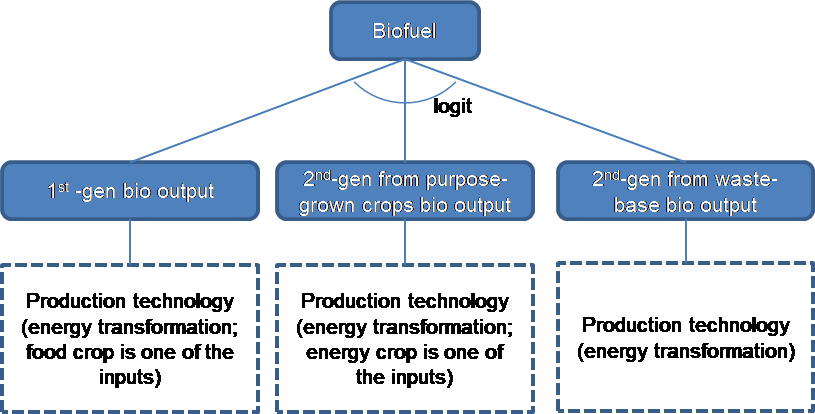
\includegraphics[width=1\textwidth]{fig/image19.png}
\caption{{Biomass supply}\label{ref-0145}}
\label{fig:9}
\end{figure}
\subsection{\label{subsec:OthEneTraSec}{Other energy transformation sectors}}

Other than those of energy transformation sectors such as petroleum refineries and town gas distribution sectors assumed to keep the same production structure as shown in power sector. It's input coefficients are also constant including energy transformation efficiency.

\section{\label{sec:EneDem}{Energy demand}}

The energy demand, in this document, is classified as final energy consumption defined in energy balance table (International Energy Agency 2018)~\cite{RN3606}. It generally consists of five or six sectors; industry, transportation, residential, commercial, non-energy use and other sectors\footnote{Residential and commercial are sometimes treated as single aggregated building sector.}. Actual AIM/CGE has more disaggregated sectors and for example iron and steel, and food processing are classified as part of industrial sectors. The model has two options how to determine these energy demands. One is using traditional functions such as CES function for production sectors. The other option enables to consider bottom-up energy technological information and the energy demand explicitly determined by the detailed energy technologies (Fujimori et al. 2014)~\cite{RN4010}. In this section, the former method is explained.

\subsection{\label{subsec:ProSec}{Production sectors}}

\subsubsection{\label{subsubsec:TotEne}Total energy}

The general production structure of energy end-use sectors is illustrated in Figure \ref{fig:ProductionStructure}. The energy demand is associated with the bundle of value-added and energy. The aggregated energy and value-added branch is assumed a fixed coefficient to output of that sector while the energy and value-added are assumed to have substitution relationship.

There are three main factors to determine energy demand. First is the production itself and it is driven by the value-added growth which consists of labor, capital and their productivities. In other words, GDP growth drives energy demand. However, the GDP and energy demand is not linearly linked and usually energy demand growth rate is slower than GDP even the relationship of energy and value added prices are constant. This is the second factor to change the energy demand and realized by technological progress (the effect of more efficient energy device) or energy service demand efficiency improvement (e.g. floor space of office is not so expand as the economic value of output), or mixture of them. We normally call this factor as AEEI (Autonomous Energy Efficiency Improvement) and multiply coefficients to the energy efficiency. the AEEI is changed as a function of GDP growth. In principle, the AEEI is high when a country has a high GDP growth rate, whereas it is low in low GDP growth areas (van Ruijven et al. 2010). If GDP growth is negative, AEEI is fixed as zero. If GDP growth ranges from 0-3\%, 3-5\%, and over 5\%, annual AEEI is assumed to be 1\%, 1.5\%, and half of the GDP growth percentage, respectively. 

The third one is price factor. The ratio of energy and value-added inputs are determined by those of relative price relationship. The relative price and volume input relationship can be derived from the maximization profit condition subject to the CES production function. The ratio of value-added and energy is determined by the share parameters (which are usually calibrated from base year's data) and the price ratio associated with substitution elasticity.

\subsubsection{\label{subsubsec:EneMix}Energy mix}

The next story is how to determine the energy source mix to satisfy final energy demand. Energy has several forms such as solid, liquid and gaseous and so on. The energy mix is associated with each sector's activity and its technologies. For instance, the boiler could use any types of energy to obtain certain amount of energy while current car uses liquid (partly electricity and gas) but not solid type fuel. Therefore, the energy source mix is not determined by simple cost minimization mechanism. However, the relatively cheaper energy sources may be attractive than others. To meet these mechanisms and to keep simplicity to solve the large system equilibrium model, the energy source mix is assumed to be determined by the CES function. The elasticity of substitution among the energy forms is 2.0 (Figure 13.3). The AEEI should differ across energy sources to reflect the energy consumption composite switch from coal to oil, gas, or electricity. Therefore, coal, gas, and electricity are assumed to have 1\%, -0.5\%, and -1\% annual changes. Because previous studies did not report these values, these numbers are arbitrarily assigned. The AEEI for the traditional biomass usage was assumed to be 1\% annually.

\subsection{\label{subsec:ResSec}{Residential sectors}}

The household consumption is determined by the LES as explained earlier. The energy demand is treated as two kinds of household goods. One is associated with the car usage energy demand and the other is rest of the energy demand. There is a definition difference between energy balance table and social accounting matrix in terms of how to account the energy consumption by private household cars. The social accounting matrix deals with the fuel consumption in order to drive household car is accounted as part of household consumption while energy balance treats it as transport sector's energy consumption. To deal with the household energy demand consistently, we separately treat the car fuel and rest of energy.

The total car energy consumptions or other energy demand are determined goods prices and income of household under LES. We basically assumed 1.0 and 0.5 as income elasticity for the car energy usage and rest of household energy consumption. The income elasticity can be derived from the LES function and it is fixed assumption for the future simulation. However, the derived income elasticity depends on the parameter $\beta _{r,ch,h}^{m}$ and goods prices. In order to realize the constant income elasticity, the parameters are calibrated recursively.

Energy source mix is determined by logit function for each energy demand. The structure of household energy demand is shown in Figure \ref{fig:HouDemStr}. The exponent parameters for the car fuel are -1.0 and those of other energy demand are 0.2.
\begin{figure}
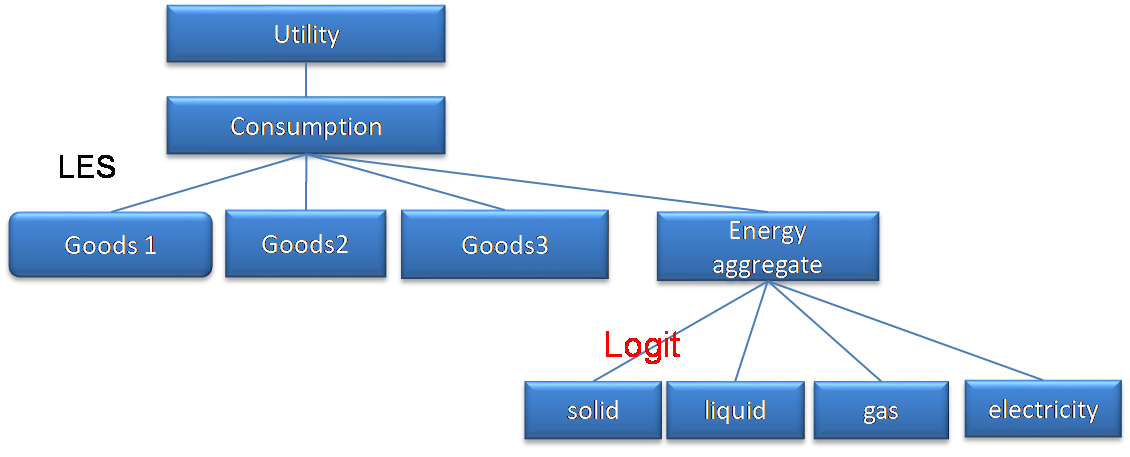
\includegraphics[width=1\textwidth]{fig/image20.png}
\caption{Household demand structure\label{fig:HouDemStr}}
\end{figure}
Currently in the energy balance table does not account electricity consumption for road transport. However, electric vehicle could be one of the options in the future. Hence, the share parameter of the logit function is updated in the future. So in year 2015 the electric vehicle is assumed to start and at that year 0.1\% of the share is assumed. This share is used for the logit functions' share parameter. Then, after that year the share parameter is linearly changed according to the electricity price. The biofuel for road transport is also similarly treaded, but the starting year is 2006.

\section{\label{sec:AgrLanUse}{Agriculture and land use}}

Regarding with agriculture and land use there three topics should be discussed in this section. First is how the agricultural commodities' productions are determined. Second is the demand side story. How the demand is modeled and trade is also included. Third, the production side has land completion and how the land completion is realized within this model is explained.

\subsection{\label{subsec:AgrComPro}{Agricultural commodities production}}

Producers are assumed to maximize profits subject to technology (production functions) and prices of inputs. The first-order conditions for profit maximization essentially define the factor demands and output supply behavior of producers. The production structure is same as other industrial sectors except for land input treatment. The land input is assumed multiplying a coefficient to output. However, in some cases this fixed coefficient approach makes difficult to solve the program if the land constraint is substantially critical. Therefore, the term related to output price elasticity is multiplied to the fixed coefficient. The price elasticity is very small (say 0.05) and the model results can be interpreted as the land input is almost treated as Leontief type input. Whether the treatment that land input is fixed technology has reality or not should be concerned carefully. The main technologies related to improving land efficiency are fertilizer inputs, advanced cultivar, optimizing planting date and irrigation. When we consider the climate change impact, the constraints caused by climate change are water and temperature. These conditions can be partly controlled by the latter three technologies. The cultivars and planting date are what we call autonomous adaptation and it would not change the production cost so much. GAEZ (Masutomi et al. 2009)~\cite{RN2253} results are usually fed into this CGE model to analyze climate change impact and within GAEZ framework the cultivars and planting date are already considered. Therefore, the last irrigation is the remained technology which could change the yield and production cost. However, the irrigation is not always accounted as production cost but as social infrastructure (reservoirs and canal). It makes difficult to analyze the relationship of production cost and irrigation technologies. Tentatively, we don't touch about this issue in this version but we need to consider this limitation to interpret the results of this model.

The future land input coefficient, which is yield, is exogenous assumption and based on IFPRI's IMAPCT (Msangi et al. 2010)~\cite{RN2538} and Table \ref{tab:FutYieAss} shows actual numbers used in the default scenario. It does not include climate change impact.

The livestock land productivity is assumed to be corresponding to the livestock goods demand change. For instance, if the meet demand is supposed to be 1.5 folds, then its land productivity is also assumed as well. This mechanism is based on the historical evidence that we could not find any relationship between grazing land productivity and other factors like economic development level whereas the grazing area looked rather constant.


\begin{tabularx}{\textwidth}{|
p{\dimexpr 0.108\linewidth-2\tabcolsep-2\arrayrulewidth}|
p{\dimexpr 0.11\linewidth-2\tabcolsep-\arrayrulewidth}|
p{\dimexpr 0.118\linewidth-2\tabcolsep-\arrayrulewidth}|
p{\dimexpr 0.24\linewidth-2\tabcolsep-\arrayrulewidth}|
p{\dimexpr 0.178\linewidth-2\tabcolsep-\arrayrulewidth}|
p{\dimexpr 0.246\linewidth-2\tabcolsep-\arrayrulewidth}|} 
\caption{\label{tab:FutYieAss}Future yield assumptions}\\
\hline 
 & Rice & Wheat & Other grains & Oil crops & Sugar crops \\\hline 
USA & 0.7\% & 1.0\% & 1.1\% & 0.8\% & 0.7\% \\\hline 
XE25 & 1.2\% & 0.3\% & 0.8\% & 0.9\% & 0.4\% \\\hline 
XER & 1.0\% & 1.3\% & 1.3\% & 1.4\% & 1.1\% \\\hline 
TUR & 0.2\% & 1.0\% & 0.7\% & 0.5\% & 1.1\% \\\hline 
XOC & 0.1\% & 1.0\% & 1.3\% & 0.6\% & 0.4\% \\\hline 
CHN & 0.8\% & 0.9\% & 1.5\% & 1.0\% & 0.9\% \\\hline 
IND & 1.3\% & 0.8\% & 2.1\% & 0.8\% & 0.5\% \\\hline 
JPN & 0.3\% & 0.6\% & 0.6\% & 0.2\% & 0.6\% \\\hline 
XSE & 1.0\% & 1.8\% & 1.4\% & -0.4\% & 0.8\% \\\hline 
XSA & 0.9\% & 1.4\% & 1.4\% & 0.9\% & 1.4\% \\\hline 
CAN & - & 1.8\% & 1.6\% & 0.1\% & 1.0\% \\\hline 
BRA & 0.8\% & 1.7\% & 1.8\% & 0.9\% & 1.1\% \\\hline 
XLM & 0.6\% & 1.3\% & 1.4\% & 0.6\% & 1.1\% \\\hline 
CIS & 1.7\% & 2.0\% & 2.1\% & 1.4\% & 1.4\% \\\hline 
XME & 1.2\% & 2.2\% & 2.0\% & 1.0\% & 1.1\% \\\hline 
XNF & 0.7\% & 1.3\% & 1.3\% & 1.3\% & 0.8\% \\\hline 
XAF & 2.0\% & 2.1\% & 1.5\% & 0.9\% & 0.8\% \\\hline 
\end{tabularx}

\subsection{\label{subsec:DemAgrCom}Demand of agricultural commodities}

As section \ref{subsec:PopLabPar} shows, the household expenditure is represented by LES function. The parameters dealt with LES are changed overtime.

At least food related goods are crucial for this model, their parameters are carefully treated, since they are physically accounted in this model. We assumed food consumption income elasticity according to two sources. One is the historical observation. If we could find the relationship between the income level and food consumption, then that relationship is adopted. For the other goods we follow FAO's perspective~\cite{RN2725}. The livestock goods are former cases and one of the examples is plotted in Figure \ref{fig:MeatCal}. The latter goods income elasticity is shown in Table \ref{tab:IncElaCro}.
\begin{figure}
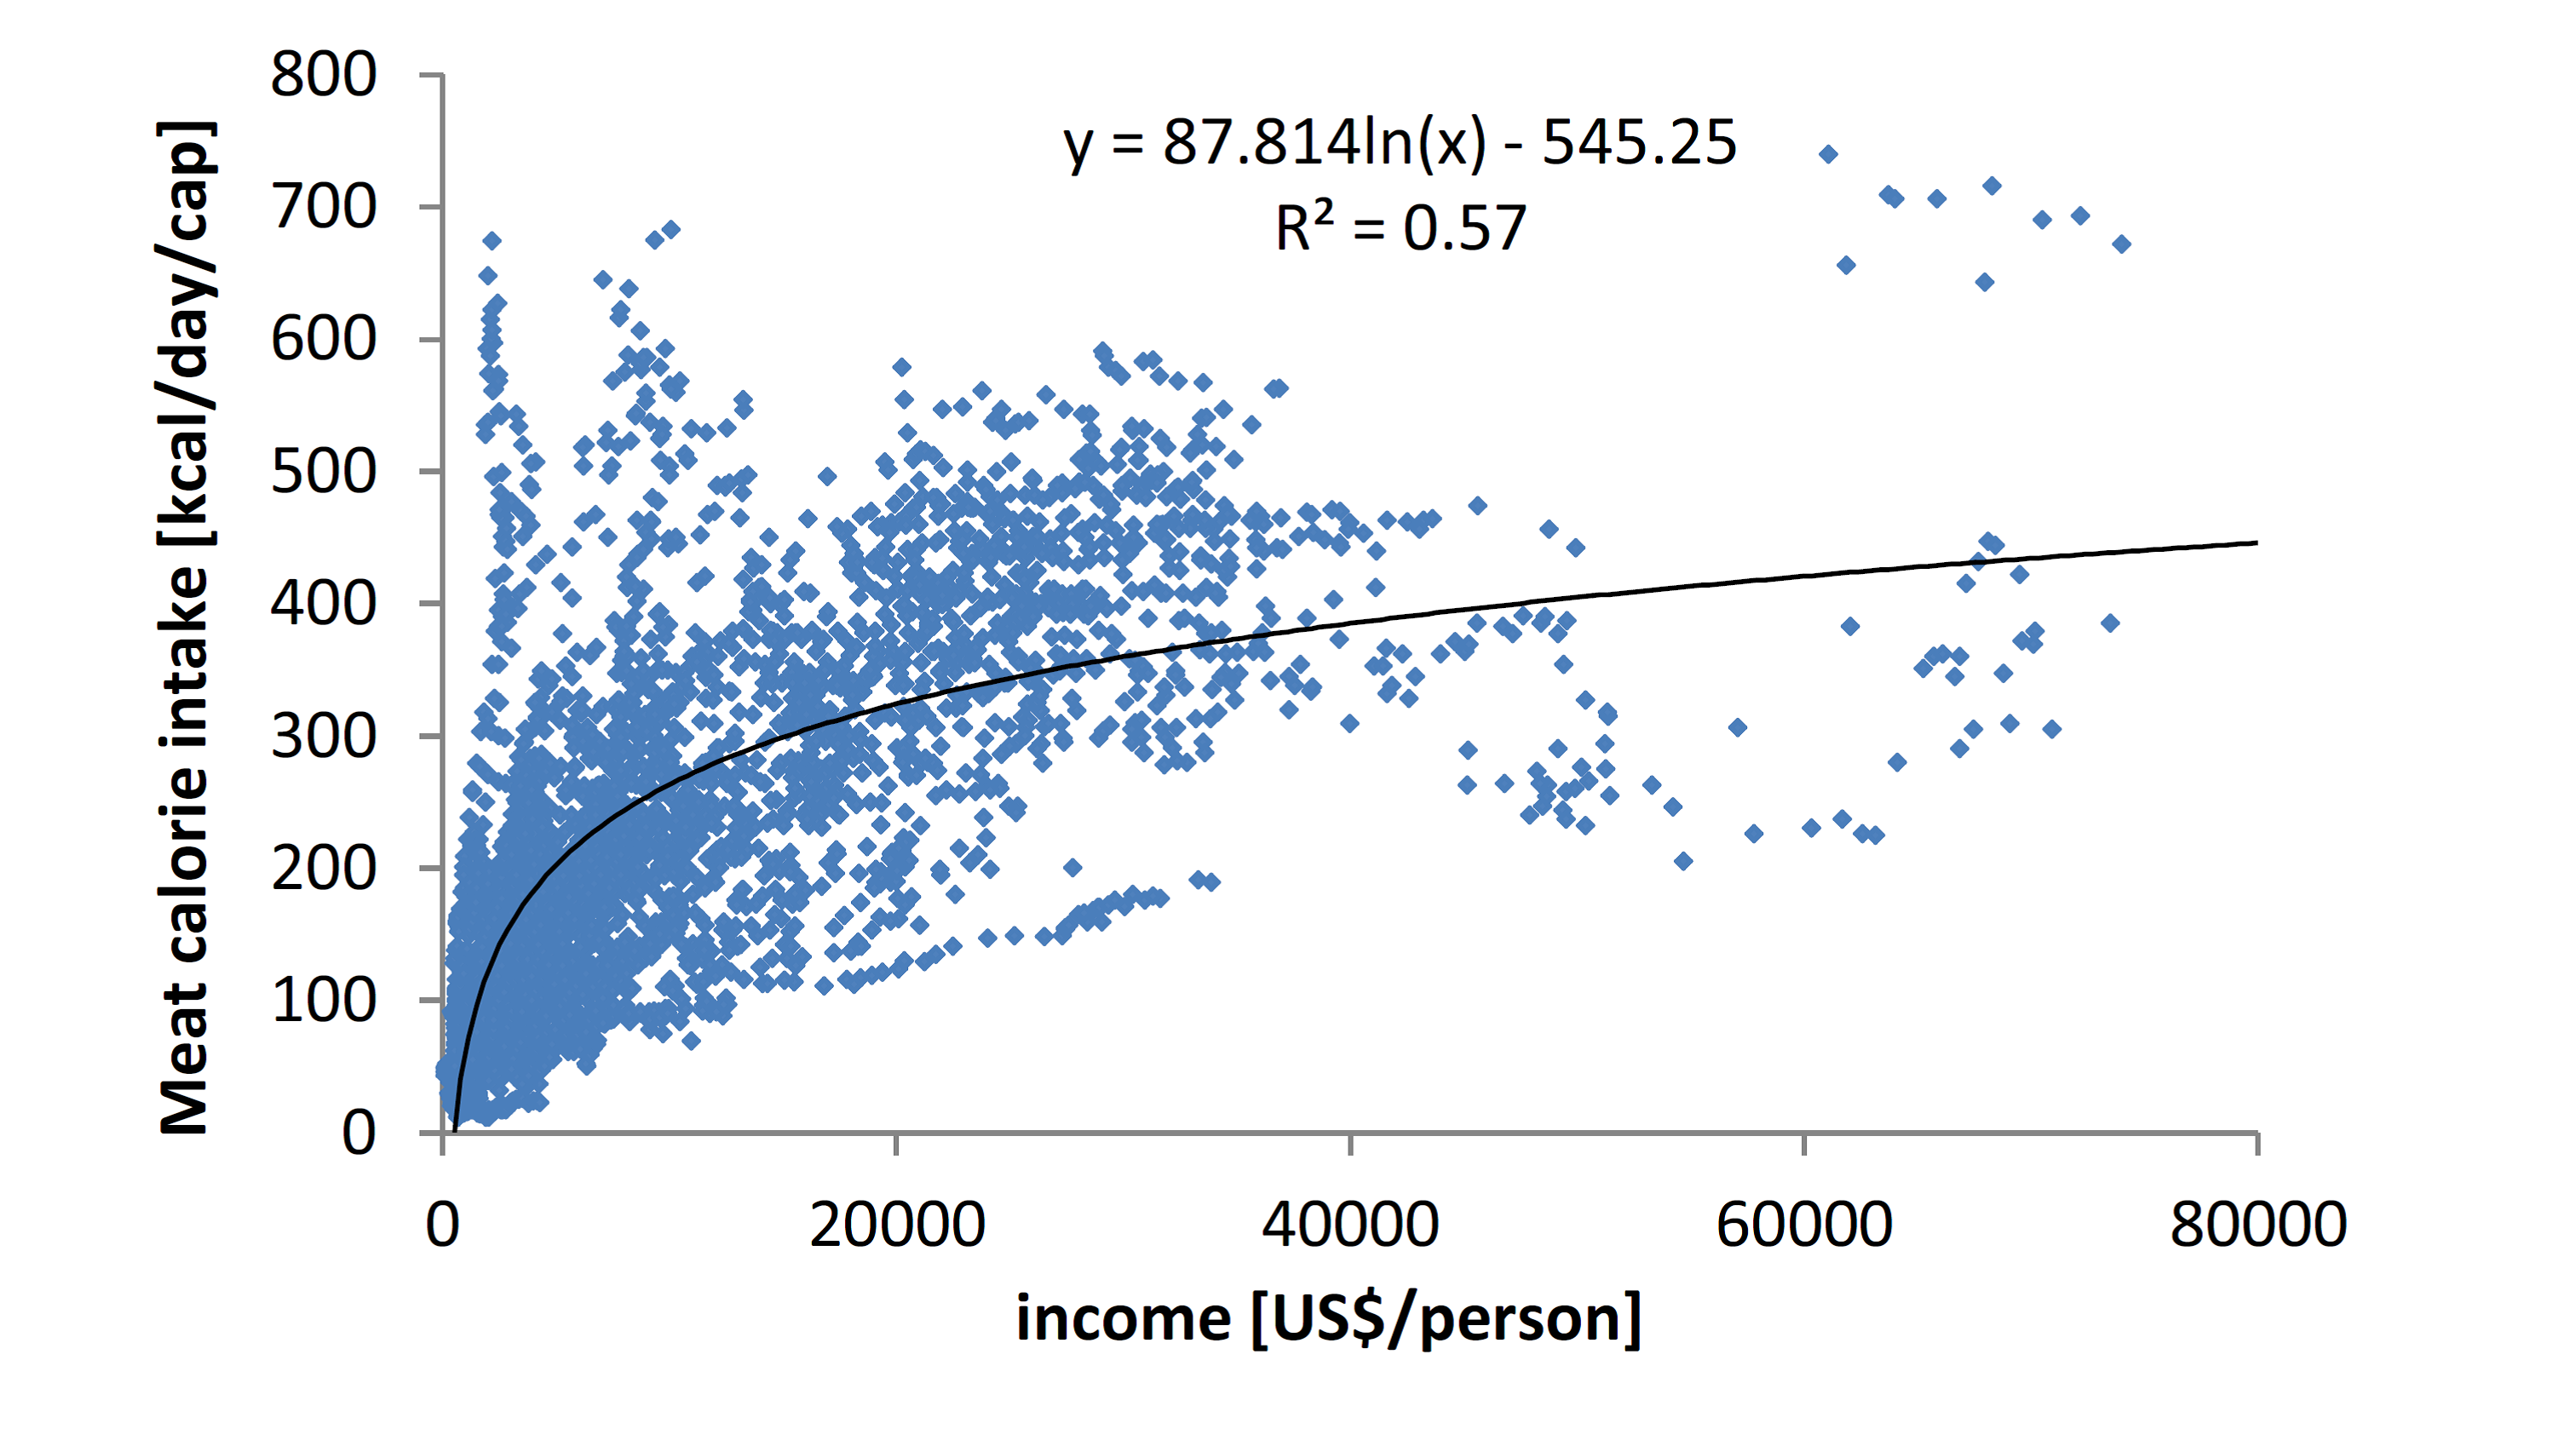
\includegraphics[width=1\textwidth]{fig/image21.png}
\caption{Time-series and cross-country data on meat calorie intake and income (1980-2009, source: World Bank (2013)~\cite{RN3647} for income and Food and Agriculture Organization of the United Nations (2013)~\cite{RN3272} for calorie intake)}
\label{fig:MeatCal}
\end{figure}

\begin{tabularx}{\textwidth}{|
p{\dimexpr 0.124\linewidth-2\tabcolsep-2\arrayrulewidth}|
p{\dimexpr 0.139\linewidth-2\tabcolsep-\arrayrulewidth}|
p{\dimexpr 0.199\linewidth-2\tabcolsep-\arrayrulewidth}|
p{\dimexpr 0.23\linewidth-2\tabcolsep-\arrayrulewidth}|
p{\dimexpr 0.307\linewidth-2\tabcolsep-\arrayrulewidth}|} 
\caption{\label{tab:IncElaCro}Income elasticity of crop consumption}\\
\hline 
 & Cereal & Oil crops & Sugar crops & Other crops \\\hline 
USA & -0.04 & 0.10 & -0.03 & -0.14 \\\hline 
XE25 & -0.04 & 0.10 & -0.03 & -0.14 \\\hline 
XER & -0.03 & 0.27 & 0.05 & -0.04 \\\hline 
TUR & -0.02 & 0.10 & 0.04 & -0.01 \\\hline 
XOC & -0.04 & 0.10 & -0.03 & -0.14 \\\hline 
CHN & -0.06 & 0.19 & 0.22 & -0.09 \\\hline 
IND & 0.03 & 0.26 & 0.10 & 0.18 \\\hline 
JPN & -0.04 & 0.10 & -0.03 & -0.14 \\\hline 
XSE & -0.01 & 0.23 & 0.12 & 0.08 \\\hline 
XSA & 0.03 & 0.26 & 0.10 & 0.18 \\\hline 
CAN & -0.04 & 0.10 & -0.03 & -0.14 \\\hline 
BRA & 0.04 & 0.24 & -0.02 & -0.07 \\\hline 
XLM & 0.04 & 0.24 & -0.02 & -0.07 \\\hline 
CIS & -0.03 & 0.27 & 0.05 & -0.04 \\\hline 
XME & -0.04 & 0.16 & 0.06 & -0.02 \\\hline 
XNF & -0.04 & 0.16 & 0.06 & -0.02 \\\hline 
XAF & 0.22 & 0.37 & 0.39 & 0.07 \\\hline 
\end{tabularx}

As for intermediate inputs not used as the feeding for livestock is determined by income and price elasticities derived from the household consumption function.

\subsection{\label{subsec:LanComAlloMec}{Land competition and allocation mechanism}}

A function whereby land is an input for the production of crops and livestock products, and landowners change its use in accordance with the prices of producer goods on cropland, pastureland, and forest. The model has a land nesting strategy, which is similar to the treatment in  Sands and Edmonds ~\cite{RN1860} and Wise and Calvin ~\cite{RN1597}. Land is categorized in one of three ecological zones, and there is a land market for each zone. Allocation of land by sector is formulated as a multi-nominal logit function to reflect differences in substitutability across land categories with land rent. In that, the function assumes that land owner of each region and Agro-ecological Zone (AEZ) decides land sharing among options with the land rent depending on production on each land (i.e. crops, livestock and wood products). We deal with all land excluding desert, rock, ice, tundra, and built-up land. The model has 18 AEZ classifications.

\begin{figure}
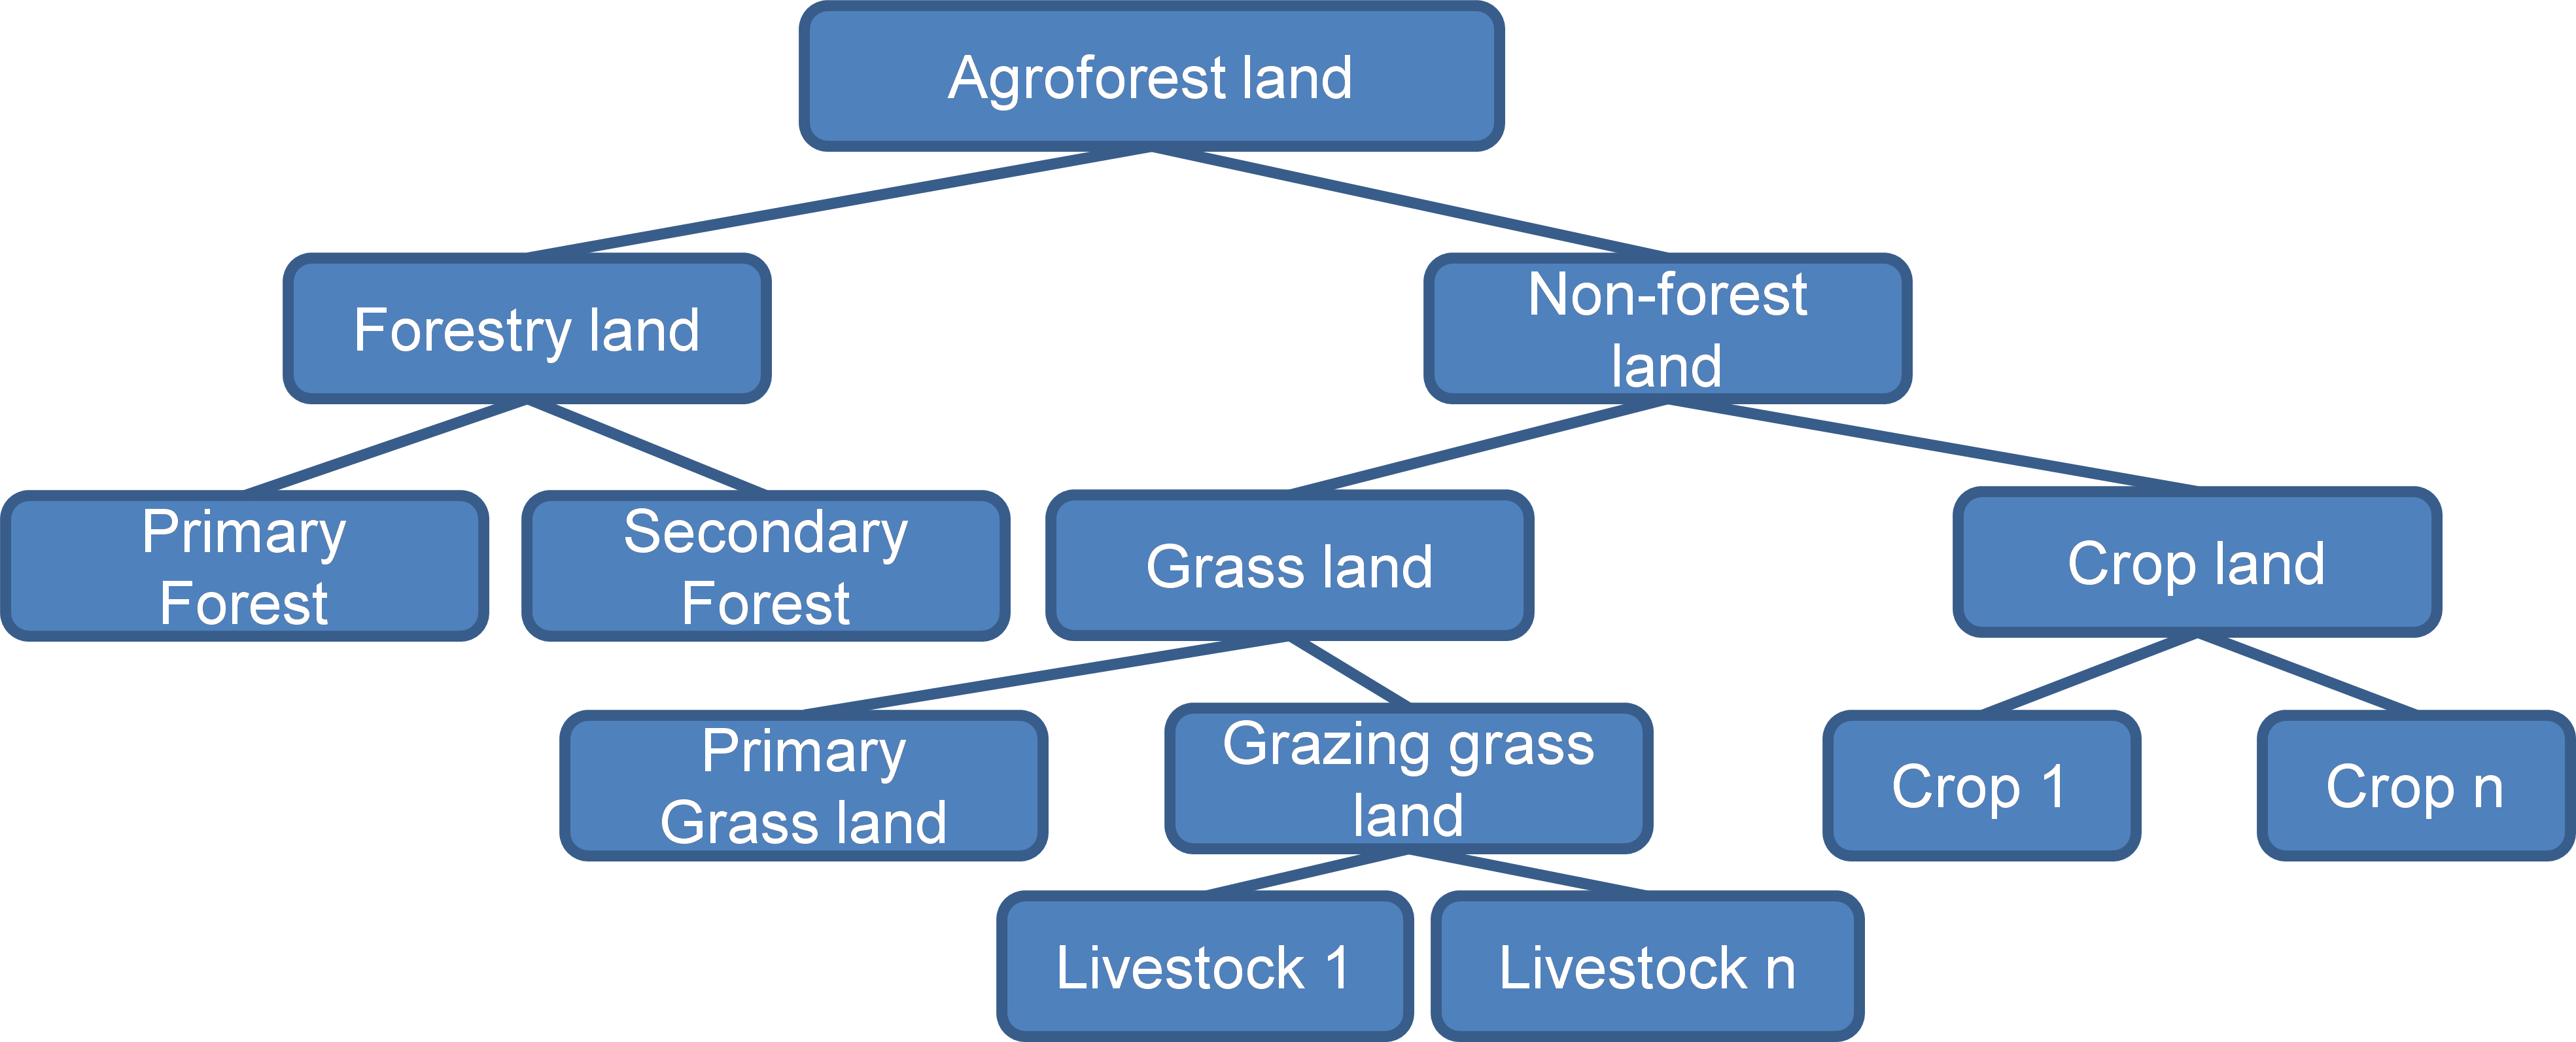
\includegraphics[width=1\textwidth]{fig/image22.png}
\label{fig:12}
\caption{\label{fig:LanAlloStr}Land allocation structure}
\end{figure}

Figure \ref{fig:LanAlloStr} shows the nesting diagram of land with an AEZ classification. We deal with all land, excluding desert, rock, ice, tundra, and built-up land. There are 18 AEZ classifications. At the top is all land, which is divided into two main types of nodes: forest land and non-forest land. The forest land node contains two competing uses: primary forest (unmanaged forest) and secondary forest (managed forest). The non-forest land could be divided; all grassland and cropland. The grassland could be divided into primary grassland (unmanaged pasture) and grazing grassland (managed pasture that which feeds marketed livestock) which is divided further into each livestock (1 to n). The cropland could be divided further into cropland for each crop (1 to n) and fallow land. One approach of the nesting strategies is based on the assumption that the land regions are small enough that all competing options are equally substitutable. This assumption implies that it is easy to switch from forest to wheat as it is to switch from corn to wheat. However, this conversion would not happen unless wheat was more profitable than forest or corn. In that, the function assumes that land owner of each region and AEZ sub-region decides land sharing among options depending on the land rent from production on each land (i.e. crops, livestock and wood products). To calibrate the function for both of the managed and unmanaged lands in the base year, we used the mean base-year land rent of the managed land as that of the unmanaged land because of unavailable data for the unmanaged land. Carbon stock on forest land is evaluated by price in the case of climate mitigation scenario. Land rent of forest includes both of revenue of wood product and the price of the carbon stock.

\section{\label{sec:GHGRedMeaOthThanCHaEneSys}{GHG reduction measures other than changing energy system}}

\subsection{\label{subsec:CCS}{CCS (Carbon Capture and Storage)}}

CCS technology is one of the key technologies for climate mitigation and this subsection explains how it is treated in the model. CCS captures the CO2 using chemical processes and stores the carbon underground or in the deep sea. It is mainly available for the large point CO2 emission sources. Fired power plants, biomass power plants, oil refineries and coal transformation plants, non-metal and mineral, chemical, and paper and pulp industries are supposed to be able to apply CCS technology in this study. These sectors input CCS services as intermediate inputs and the CCS service is assumed to be provided by a CCS service sector which has independent production function.

The costs of the technology are different among sectors and are shown in Table \ref{tab:CCSTecCos}. These costs have been taken from IEA (2008) \cite{RN2115}. Since IEA (2008)\cite{RN2115} provides a range of the cost estimates we took medium values. When the GHG emission price becomes higher than these costs, CCS technology is installed with a maximum increase ratio of 5 \% per year. CCS is assumed to be installable after 2020 since it is still under examination.


\begin{tabularx}{\textwidth}{|
p{\dimexpr 0.208\linewidth-2\tabcolsep-2\arrayrulewidth}|
p{\dimexpr 0.538\linewidth-2\tabcolsep-\arrayrulewidth}|
p{\dimexpr 0.254\linewidth-2\tabcolsep-\arrayrulewidth}|} 
\caption{\label{tab:CCSTecCos}CCS technology cost}\\
\hline 
 & sectors & price (US\$/tCO\textsubscript{2}) \\\hline 
\multirow{4}{=}{Manufacturing}  & petroleum refinery coal transformation & 100 \\\cline{2-3}
 & non-metal and mineral & 200 \\\cline{2-3}
 & paper and pulp & 150 \\\cline{2-3}
 & chemical & 150 \\\hline 
\multirow{4}{=}{Power}  & Coal fired & 100 \\\cline{2-3}
 & Oil fired & 80 \\\cline{2-3}
 & Gas fired  & 80 \\\cline{2-3}
 & Biomass fired & 80 \\\hline 
\end{tabularx}

\subsection{\label{subsec:NonCO2Red}{Non-CO2 reduction}}

As for the non-energy-related GHG emissions reductions in areas such as agricultural CH4 and N2O emissions, the following equation is used. A similar method is already discussed by Hyman et al. (2003)~\cite{RN2134}. The parameter is taken from Lucas et al. (2007)~\cite{RN2282}

\subsection{\label{subsec:LanUseRelCouMea}Land use related counter measures}

Once carbon is priced, the stock of the forestry is potentially assumed to have value. This carbon value is assumed to be additional land rent for the forestry and it makes forestry larger. The value itself is discounted carbon value. Life time of forestry that can absorb carbon is assumed as 60 years and interest rate is 5\%. The amount of carbon absorption made by afforestation is depending on the age of the trees. The carbon stock is differentiated across AEZ.

\section{\label{sec:HowImpNewProSec}How to implement new production sectors or goods (not accounted in the base year) }

The sectors or goods which are not recorded in the base year (e.g. solar power, biofuel and so on) need to be assumed explicitly in future some year. Advanced renewable energy or CCS technologies are under this treatment. The list of the sectors and goods and the starting years are shown in Table \ref{tab:LisSecGood}.


\begin{tabularx}{\textwidth}{|
p{\dimexpr 0.119\linewidth-2\tabcolsep-2\arrayrulewidth}|
p{\dimexpr 0.723\linewidth-2\tabcolsep-\arrayrulewidth}|
p{\dimexpr 0.157\linewidth-2\tabcolsep-\arrayrulewidth}|} 
\caption{\label{tab:LisSecGood}List of sectors and goods which are not accounted base year, but newly introduced in the future scenarios and the starting years}\\
\hline 
 & Goods or sectors & Starting year \\\hline 
\multirow{6}{=}{Goods}  & Biofuel & 2006 \\\cline{2-3}
 & CCS service for cement & 2021 \\\cline{2-3}
 & CCS service for furnaces & 2021 \\\cline{2-3}
 & CCS service for other manufacturing & 2021 \\\cline{2-3}
 & CCS service for coal fired power plant & 2021 \\\cline{2-3}
 & CCS service for other fired power plant and biomass refinery & 2021 \\\hline 
\multirow{8}{=}{Sectors}  & 1st -gen biofuel & 2006 \\\cline{2-3}
 & 2nd-gen biofuel from purpose grown energy crops  & 2015 \\\cline{2-3}
 & 2nd-gen biofuel from waste base & 2015 \\\cline{2-3}
 & Purpose grown energy crops & 2015 \\\cline{2-3}
 & Nuclear & 2006 \\\cline{2-3}
 & Wind & 2006 \\\cline{2-3}
 & Solar & 2006 \\\cline{2-3}
 & Biomass fired power & 2006 \\\hline 
\end{tabularx}

To implement those sectors or goods, the production input coefficients or demand of the goods should be formulated. The same production structures as those of US are assumed for the nuclear, renewable power energies. The coefficients of the production are shown in Table \ref{tab:InpCoePowGen} for power generation. The demand of the generated power is assumed very small portion in the starting year (0.1\% of the total generation) and this assumption is made on the share parameter.

The CCS technologies inputs four factors as labor, capital, chemical products, transport, and other services. The cost shares are assumed 0.1, 0.4, 0.1, 0.3 and 0.1 respectively. The assumed input coefficients are based on (IEA 2008).


\begin{tabularx}{\textwidth}{|
p{\dimexpr 0.319\linewidth-2\tabcolsep-2\arrayrulewidth}|
p{\dimexpr 0.153\linewidth-2\tabcolsep-\arrayrulewidth}|
p{\dimexpr 0.153\linewidth-2\tabcolsep-\arrayrulewidth}|
p{\dimexpr 0.153\linewidth-2\tabcolsep-\arrayrulewidth}|
p{\dimexpr 0.223\linewidth-2\tabcolsep-\arrayrulewidth}|} 
\caption{\label{tab:InpCoePowGen}Input coefficients for power generation (thousand \$ per toe of electricity production).}\footnote{Electricity and energy crop inputs are accounted as toe per toe of electricity production} \\
\hline 
 & Nuclear & Solar & Wind & Biomass fired \\\hline 
Energy crops* &  &  &  & 2.5 \\\hline 
Other manufacturing & 0.022 & 0.027 & 0.027 & 0.058 \\\hline 
Electricity* & 0.067 &  &  &  \\\hline 
Construction & 0.041 & 0.049 & 0.049 & 0.099 \\\hline 
Transport & 0.068 & 0.081 & 0.080 & 0.161 \\\hline 
Other services & 0.106 & 0.126 & 0.125 & 0.250 \\\hline 
Labor & 0.095 & 0.113 & 0.113 & 0.226 \\\hline 
Capital & 0.545 & 0.537 & 0.538 & 0.206 \\\hline 
\end{tabularx}


\noindent
\bibliographystyle{naturemag}
\bibliography{EndNoteLibrary}

\chapter{\label{chp:appSupMAC}Appendix I (Marginal abatement cost and reduction cost in non-energy emissions)}

The marginal abatement cost is represented as equation \(EFFIMPR\_PRICE\_CONS\). The total abatement cost can be represented by the following equation.
To simplify the expression, $ABTC\_NCS_{r,a,g,emsc}$, $PGHG$, $NERED$ and $\sigma_{r,a,g,emsc}^{ghg}$ are shortened as Z, P, X and $\sigma$

\begin{equation}
\begin{split}
Z &= \int_{0}^{X_{0}} P dX \\
&=\int_{0}^{X_{0}} {(1-X)^{-1/\sigma}-1} dX \\
&=\left\lbrack \left(-1/\sigma+1\right)^{-1}(-1)(1-X)^{-1/\sigma+1}-X\right\rbrack_{0}^{X_{0}} \\
&=\left\lbrack \left(\frac{\sigma}{1-\sigma}\right)(1-X)^{\left(\frac{\sigma-1}{\sigma}\right)}-X \right\rbrack_{0}^{X_{0}} \\
&=\left(\frac{\sigma}{1-\sigma}\right)\left(1-X_{0}\right)^{\left(\frac{\sigma-1}{\sigma}\right)}-X_{0} - \frac{\sigma}{1-\sigma} 
\end{split}
\notag\end{equation}

This integration is applied to the baseline emissions and thus $E(1-X)^{(-1)}$ should be muliplied.


\chapter{\label{chp:appCountryList}Appendix II (List of coutries and mapping with global 17 regions)}
\begin{tabularx}{\textwidth}{|
p{\dimexpr 0.18\linewidth-2\tabcolsep-2\arrayrulewidth}|
p{\dimexpr 0.369\linewidth-2\tabcolsep-\arrayrulewidth}|
p{\dimexpr 0.108\linewidth-2\tabcolsep-\arrayrulewidth}|
p{\dimexpr 0.4\linewidth-2\tabcolsep-\arrayrulewidth}|} 
\caption{List of countries}\label{tab:List of countries}\\
 \\
 \hline
\textbf{Native Region Code } & \textbf{Native Region Name} & \textbf{ISO Code} & \textbf{Country} \\ \hline\hline
 \endfirsthead
 \multicolumn{4}{l}{\small\it Continued from previous page}\\
 \hline
\textbf{Native Region Code } & \textbf{Native Region Name} & \textbf{ISO Code} & \textbf{Country} \\  \hline\hline
 \endhead
 \hline
 \multicolumn{4}{l}{\small\it Continue to next page}\\
 \endfoot
 \hline
 \multicolumn{4}{l}{\small\it end }\\
 \endlastfoot

XLM & Rest of Brazil & ABW & Aruba~ \\\hline 
XSA & Rest of Asia & AFG & Afghanistan~ \\\hline 
XAF & Other Africa & AGO & Angola~ \\\hline 
XLM & Rest of Brazil & AIA & Anguilla~ \\\hline 
\#N/A & \#N/A & ALA & \AA{}land Islands~ \\\hline 
XER & Rest of Europe & ALB & Albania~ \\\hline 
XER & Rest of Europe & AND & Andorra~ \\\hline 
XLM & Rest of Brazil & ANT & Netherlands Antilles~ \\\hline 
XME & Middle East & ARE & United Arab Emirates~ \\\hline 
XLM & Rest of Brazil & ARG & Argentina~ \\\hline 
CIS & Former USSR & ARM & Armenia~ \\\hline 
XSA & Rest of Asia & ASM & American Samoa~ \\\hline 
\#N/A & \#N/A & ATA & Antarctica~ \\\hline 
XSA & Rest of Asia & ATF & French Southern Territories~ \\\hline 
XLM & Rest of Brazil & ATG & Antigua and Barbuda~ \\\hline 
XOC & New Zealand and Australia & AUS & Australia~ \\\hline 
XE25 & EU & AUT & Austria~ \\\hline 
CIS & Former USSR & AZE & Azerbaijan~ \\\hline 
XAF & Other Africa & BDI & Burundi~ \\\hline 
XE25 & EU & BEL & Belgium~ \\\hline 
XAF & Other Africa & BEN & Benin~ \\\hline 
XAF & Other Africa & BFA & Burkina Faso~ \\\hline 
XSA & Rest of Asia & BGD & Bangladesh~ \\\hline 
XER & Rest of Europe & BGR & Bulgaria~ \\\hline 
XME & Middle East & BHR & Bahrain~ \\\hline 
XLM & Rest of Brazil & BHS & Bahamas~ \\\hline 
XER & Rest of Europe & BIH & Bosnia and Herzegovina~ \\\hline 
\#N/A & \#N/A & BLM & Saint Barth\'{e}lemy~ \\\hline 
CIS & Former USSR & BLR & Belarus~ \\\hline 
XLM & Rest of Brazil & BLZ & Belize~ \\\hline 
XLM & Rest of Brazil & BMU & Bermuda~ \\\hline 
XLM & Rest of Brazil & BOL & Bolivia, Plurinational State of~ \\\hline 
BRA & Brazil & BRA & Brazil~ \\\hline 
XLM & Rest of Brazil & BRB & Barbados~ \\\hline 
XSA & Rest of Asia & BRN & Brunei Darussalam~ \\\hline 
XSA & Rest of Asia & BTN & Bhutan~ \\\hline 
XLM & Rest of Brazil & BVT & Bouvet Island~ \\\hline 
XAF & Other Africa & BWA & Botswana~ \\\hline 
XAF & Other Africa & CAF & Central African Republic~ \\\hline 
CAN & Canada & CAN & Canada~ \\\hline 
XSA & Rest of Asia & CCK & Cocos (Keeling) Islands~ \\\hline 
XER & Rest of Europe & CHE & Switzerland~ \\\hline 
XLM & Rest of Brazil & CHL & Chile~ \\\hline 
CHN & China & CHN & China~ \\\hline 

XAF & Other Africa & CIV & C\^{o}te d'Ivoire~ \\\hline 
XAF & Other Africa & CMR & Cameroon~ \\\hline 
XAF & Other Africa & COD & Congo, the Democratic Republic of the~ \\\hline 
XAF & Other Africa & COG & Congo~ \\\hline 
XSA & Rest of Asia & COK & Cook Islands~ \\\hline 
XLM & Rest of Brazil & COL & Colombia~ \\\hline 
XAF & Other Africa & COM & Comoros~ \\\hline 
XAF & Other Africa & CPV & Cape Verde~ \\\hline 
XLM & Rest of Brazil & CRI & Costa Rica~ \\\hline 
XLM & Rest of Brazil & CUB & Cuba~ \\\hline 
XSA & Rest of Asia & CXR & Christmas Island~ \\\hline 
XLM & Rest of Brazil & CYM & Cayman Islands~ \\\hline 
XE25 & EU & CYP & Cyprus~ \\\hline 
XE25 & EU & CZE & Czech Republic~ \\\hline 
XE25 & EU & DEU & Germany~ \\\hline 
XAF & Other Africa & DJI & Djibouti~ \\\hline 
XLM & Rest of Brazil & DMA & Dominica~ \\\hline 
XE25 & EU & DNK & Denmark~ \\\hline 
XLM & Rest of Brazil & DOM & Dominican Republic~ \\\hline 
XNF & North Africa & DZA & Algeria~ \\\hline 
XLM & Rest of Brazil & ECU & Ecuador~ \\\hline 
XNF & North Africa & EGY & Egypt~ \\\hline 
XAF & Other Africa & ERI & Eritrea~ \\\hline 
XAF & Other Africa & ESH & Western Sahara~ \\\hline 
XE25 & EU & ESP & Spain~ \\\hline 
XE25 & EU & EST & Estonia~ \\\hline 
XAF & Other Africa & ETH & Ethiopia~ \\\hline 
XE25 & EU & FIN & Finland~ \\\hline 
XSA & Rest of Asia & FJI & Fiji~ \\\hline 
XLM & Rest of Brazil & FLK & Falkland Islands (Malvinas)~ \\\hline 
XE25 & EU & FRA & France~ \\\hline 
XER & Rest of Europe & FRO & Faroe Islands~ \\\hline 
XSA & Rest of Asia & FSM & Micronesia, Federated States of~ \\\hline 
XAF & Other Africa & GAB & Gabon~ \\\hline 
XE25 & EU & GBR & United Kingdom~ \\\hline 
CIS & Former USSR & GEO & Georgia~ \\\hline 
\#N/A & \#N/A & GGY & Guernsey~ \\\hline 
XAF & Other Africa & GHA & Ghana~ \\\hline 
XER & Rest of Europe & GIB & Gibraltar~ \\\hline 
XAF & Other Africa & GIN & Guinea~ \\\hline 
XLM & Rest of Brazil & GLP & Guadeloupe~ \\\hline 
XAF & Other Africa & GMB & Gambia~ \\\hline 
XAF & Other Africa & GNB & Guinea-Bissau~ \\\hline 
XAF & Other Africa & GNQ & Equatorial Guinea~ \\\hline 
XE25 & EU & GRC & Greece~ \\\hline 
XLM & Rest of Brazil & GRD & Grenada~ \\\hline 
XLM & Rest of Brazil & GRL & Greenland~ \\\hline 
XLM & Rest of Brazil & GTM & Guatemala~ \\\hline 
XLM & Rest of Brazil & GUF & French Guiana~ \\\hline 
XSA & Rest of Asia & GUM & Guam~ \\\hline 

XLM & Rest of Brazil & GUY & Guyana~ \\\hline 
CHN & China & HKG & Hong Kong~ \\\hline 
XSA & Rest of Asia & HMD & Heard Island and McDonald Islands~ \\\hline 
XLM & Rest of Brazil & HND & Honduras~ \\\hline 
XER & Rest of Europe & HRV & Croatia~ \\\hline 
XLM & Rest of Brazil & HTI & Haiti~ \\\hline 
XE25 & EU & HUN & Hungary~ \\\hline 
XSE & Rest of East and South East Asia & IDN & Indonesia~ \\\hline 
\#N/A & \#N/A & IMN & Isle of Man~ \\\hline 
IND & India & IND & India~ \\\hline 
XSA & Rest of Asia & IOT & British Indian Ocean Territory~ \\\hline 
XE25 & EU & IRL & Ireland~ \\\hline 
XME & Middle East & IRN & Iran, Islamic Republic of~ \\\hline 
XME & Middle East & IRQ & Iraq~ \\\hline 
XER & Rest of Europe & ISL & Iceland~ \\\hline 
XME & Middle East & ISR & Israel~ \\\hline 
XE25 & EU & ITA & Italy~ \\\hline 
XLM & Rest of Brazil & JAM & Jamaica~ \\\hline 
\#N/A & \#N/A & JEY & Jersey~ \\\hline 
XME & Middle East & JOR & Jordan~ \\\hline 
JPN & Japan & JPN & Japan~ \\\hline 
CIS & Former USSR & KAZ & Kazakhstan~ \\\hline 
XAF & Other Africa & KEN & Kenya~ \\\hline 
CIS & Former USSR & KGZ & Kyrgyzstan~ \\\hline 
XSE & Rest of East and South East Asia & KHM & Cambodia~ \\\hline 
XSA & Rest of Asia & KIR & Kiribati~ \\\hline 
XLM & Rest of Brazil & KNA & Saint Kitts and Nevis~ \\\hline 
XSE & Rest of East and South East Asia & KOR & Korea, Republic of~ \\\hline 
XME & Middle East & KWT & Kuwait~ \\\hline 
XSE & Rest of East and South East Asia & LAO & Lao People's Democratic Republic~ \\\hline 
XME & Middle East & LBN & Lebanon~ \\\hline 
XAF & Other Africa & LBR & Liberia~ \\\hline 
XNF & North Africa & LBY & Libyan Arab Jamahiriya~ \\\hline 
XLM & Rest of Brazil & LCA & Saint Lucia~ \\\hline 
XER & Rest of Europe & LIE & Liechtenstein~ \\\hline 
XSA & Rest of Asia & LKA & Sri Lanka~ \\\hline 
XAF & Other Africa & LSO & Lesotho~ \\\hline 
XE25 & EU & LTU & Lithuania~ \\\hline 
XE25 & EU & LUX & Luxembourg~ \\\hline 
XE25 & EU & LVA & Latvia~ \\\hline 
\#N/A & \#N/A & MAC & Macao~ \\\hline 
\#N/A & \#N/A & MAF & Saint Martin (French part)~ \\\hline 
XNF & North Africa & MAR & Morocco~ \\\hline 
XER & Rest of Europe & MCO & Monaco~ \\\hline 

CIS & Former USSR & MDA & Moldova, Republic of~ \\\hline 
XAF & Other Africa & MDG & Madagascar~ \\\hline 
XSA & Rest of Asia & MDV & Maldives~ \\\hline 
XLM & Rest of Brazil & MEX & Mexico~ \\\hline 
XSA & Rest of Asia & MHL & Marshall Islands~ \\\hline 
XER & Rest of Europe & MKD & Macedonia, the former Yugoslav Republic of~ \\\hline 
XAF & Other Africa & MLI & Mali~ \\\hline 
XE25 & EU & MLT & Malta~ \\\hline 
XSE & Rest of East and South East Asia & MMR & Myanmar~ \\\hline 
XER & Rest of Europe & MNE & Montenegro~ \\\hline 
XSE & Rest of East and South East Asia & MNG & Mongolia~ \\\hline 
XSA & Rest of Asia & MNP & Northern Mariana Islands~ \\\hline 
XAF & Other Africa & MOZ & Mozambique~ \\\hline 
XAF & Other Africa & MRT & Mauritania~ \\\hline 
XLM & Rest of Brazil & MSR & Montserrat~ \\\hline 
XLM & Rest of Brazil & MTQ & Martinique~ \\\hline 
XAF & Other Africa & MUS & Mauritius~ \\\hline 
XAF & Other Africa & MWI & Malawi~ \\\hline 
XSE & Rest of East and South East Asia & MYS & Malaysia~ \\\hline 
XAF & Other Africa & MYT & Mayotte~ \\\hline 
XAF & Other Africa & NAM & Namibia~ \\\hline 
XSA & Rest of Asia & NCL & New Caledonia~ \\\hline 
XAF & Other Africa & NER & Niger~ \\\hline 
XSA & Rest of Asia & NFK & Norfolk Island~ \\\hline 
XAF & Other Africa & NGA & Nigeria~ \\\hline 
XLM & Rest of Brazil & NIC & Nicaragua~ \\\hline 
XSA & Rest of Asia & NIU & Niue~ \\\hline 
XE25 & EU & NLD & Netherlands~ \\\hline 
XER & Rest of Europe & NOR & Norway~ \\\hline 
XSA & Rest of Asia & NPL & Nepal~ \\\hline 
XSA & Rest of Asia & NRU & Nauru~ \\\hline 
XOC & New Zealand and Australia & NZL & New Zealand~ \\\hline 
XME & Middle East & OMN & Oman~ \\\hline 
XSA & Rest of Asia & PAK & Pakistan~ \\\hline 
XLM & Rest of Brazil & PAN & Panama~ \\\hline 
XSA & Rest of Asia & PCN & Pitcairn~ \\\hline 
XLM & Rest of Brazil & PER & Peru~ \\\hline 
XSE & Rest of East and South East Asia & PHL & Philippines~ \\\hline 
XSA & Rest of Asia & PLW & Palau~ \\\hline 
XSA & Rest of Asia & pdf & Papua New Guinea~ \\\hline 
XE25 & EU & POL & Poland~ \\\hline 
XLM & Rest of Brazil & PRI & Puerto Rico~ \\\hline 
XSE & Rest of East and South East Asia & PRK & Korea, Democratic People's Republic of~ \\\hline 
XE25 & EU & PRT & Portugal~ \\\hline 

XLM & Rest of Brazil & PRY & Paraguay~ \\\hline 
\#N/A & \#N/A & PSE & Palestinian Territory, Occupied~ \\\hline 
XSA & Rest of Asia & PYF & French Polynesia~ \\\hline 
XME & Middle East & QAT & Qatar~ \\\hline 
XAF & Other Africa & REU & R\'{e}union~ \\\hline 
XER & Rest of Europe & ROU & Romania~ \\\hline 
CIS & Former USSR & RUS & Russian Federation~ \\\hline 
XAF & Other Africa & RWA & Rwanda~ \\\hline 
XME & Middle East & SAU & Saudi Arabia~ \\\hline 
XAF & Other Africa & SDN & Sudan~ \\\hline 
XAF & Other Africa & SEN & Senegal~ \\\hline 
XSE & Rest of East and South East Asia & SGP & Singapore~ \\\hline 
XLM & Rest of Brazil & SGS & South Georgia and the South Sandwich Islands~ \\\hline 
XAF & Other Africa & SHN & Saint Helena, Ascension and Tristan da Cunha~ \\\hline 
XER & Rest of Europe & SJM & Svalbard and Jan Mayen~ \\\hline 
XSA & Rest of Asia & SLB & Solomon Islands~ \\\hline 
XAF & Other Africa & SLE & Sierra Leone~ \\\hline 
XLM & Rest of Brazil & SLV & El Salvador~ \\\hline 
XER & Rest of Europe & SMR & San Marino~ \\\hline 
XAF & Other Africa & SOM & Somalia~ \\\hline 
XLM & Rest of Brazil & SPM & Saint Pierre and Miquelon~ \\\hline 
XER & Rest of Europe & SRB & Serbia~ \\\hline 
\#N/A & \#N/A & SSD & South Sudan \\\hline 
XAF & Other Africa & STP & Sao Tome and Principe~ \\\hline 
XLM & Rest of Brazil & SUR & Suriname~ \\\hline 
XE25 & EU & SVK & Slovakia~ \\\hline 
XE25 & EU & SVN & Slovenia~ \\\hline 
XE25 & EU & SWE & Sweden~ \\\hline 
XAF & Other Africa & SWZ & Swaziland~ \\\hline 
XAF & Other Africa & SYC & Seychelles~ \\\hline 
XME & Middle East & SYR & Syrian Arab Republic~ \\\hline 
XLM & Rest of Brazil & TCA & Turks and Caicos Islands~ \\\hline 
XAF & Other Africa & TCD & Chad~ \\\hline 
XAF & Other Africa & TGO & Togo~ \\\hline 
XSE & Rest of East and South East Asia & THA & Thailand~ \\\hline 
CIS & Former USSR & TJK & Tajikistan~ \\\hline 
XSA & Rest of Asia & TKL & Tokelau~ \\\hline 
CIS & Former USSR & TKM & Turkmenistan~ \\\hline 
XSE & Rest of East and South East Asia & TLS & Timor-Leste~ \\\hline 
XSA & Rest of Asia & TON & Tonga~ \\\hline 
XLM & Rest of Brazil & TTO & Trinidad and Tobago~ \\\hline 
XNF & North Africa & TUN & Tunisia~ \\\hline 
TUR & Turkey & TUR & Turkey~ \\\hline 
XSA & Rest of Asia & TUV & Tuvalu~ \\\hline 
XSE & Rest of East and South East Asia & TWN & Taiwan, Province of China~ \\\hline 
XAF & Other Africa & TZA & Tanzania, United Republic of~ \\\hline 
XAF & Other Africa & UGA & Uganda~ \\\hline 
CIS & Former USSR & UKR & Ukraine~ \\\hline
XSA & Rest of Asia & UMI & United States Minor Outlying Islands~ \\\hline 
XLM & Rest of Brazil & URY & Uruguay~ \\\hline 
USA & USA & USA & United States~ \\\hline 
CIS & Former USSR & UZB & Uzbekistan~ \\\hline 
XER & Rest of Europe & VAT & Holy See (Vatican City State)~ \\\hline 
XLM & Rest of Brazil & VCT & Saint Vincent and the Grenadines~ \\\hline 
XLM & Rest of Brazil & VEN & Venezuela, Bolivarian Republic of~ \\\hline 
XLM & Rest of Brazil & VGB & Virgin Islands, British~ \\\hline 
XLM & Rest of Brazil & VIR & Virgin Islands, U.S.~ \\\hline 
XSE & Rest of East and South East Asia & VNM & Viet Nam~ \\\hline 
XSA & Rest of Asia & VUT & Vanuatu~ \\\hline 
XSA & Rest of Asia & WLF & Wallis and Futuna~ \\\hline 
XSA & Rest of Asia & WSM & Samoa~ \\\hline 
XME & Middle East & YEM & Yemen~ \\\hline 
XAF & Other Africa & ZAF & South Africa~ \\\hline 
XAF & Other Africa & ZMB & Zambia~ \\\hline 
XAF & Other Africa & ZWE & Zimbabwe~ \\\hline 
\end{tabularx}


\end{document}
